% 高一19_延安中学_周末作业2.tex —— 高一上数学「2026-2027 年延安中学高一上周末作业 2」（试卷版/答案版）
% 试卷版：xelatex 高一19_延安中学_周末作业2.tex
% 答案版：xelatex "\def\isanswer{1}% 高一19_延安中学_周末作业2.tex —— 高一上数学「2026-2027 年延安中学高一上周末作业 2」（试卷版/答案版）
% 试卷版：xelatex 高一19_延安中学_周末作业2.tex
% 答案版：xelatex "\def\isanswer{1}% 高一19_延安中学_周末作业2.tex —— 高一上数学「2026-2027 年延安中学高一上周末作业 2」（试卷版/答案版）
% 试卷版：xelatex 高一19_延安中学_周末作业2.tex
% 答案版：xelatex "\def\isanswer{1}% 高一19_延安中学_周末作业2.tex —— 高一上数学「2026-2027 年延安中学高一上周末作业 2」（试卷版/答案版）
% 试卷版：xelatex 高一19_延安中学_周末作业2.tex
% 答案版：xelatex "\def\isanswer{1}\input{高一19_延安中学_周末作业2.tex}"
% 紧凑版：xelatex "\def\iscompact{1}\input{高一19_延安中学_周末作业2.tex}"
%
% 原始材料是微信公众号图文（公众号「魔都数学加油站」，作者署名「破晓」，
% 原文链接 https://mp.weixin.qq.com/s/tHqWSV1StO5SHSXXQ4jeUA），正文为 6 张 PNG 页；
% 原文本身就是一份**讲评版**——题目下方直接印出【答案】或【解析】。本稿把答案与解析
% 移到答案版，试卷版即一张干净的空卷；试题文字、答案与解析均照原卷录入。
%
% 与原卷的排版差异（均已在 README「说明」中交代）：
%   ① 原文自**第 3 题**起（第 1、2 题未在该文发布），源码里以 \setcounter{enumi}{2} 起编；
%      全卷只有「一、填空题」「二、解答题」两节，无选择题；
%   ② 原卷本就印有两个分节标题（已在原图上逐页放大核对过），本稿照原卷分节，只把标题改排
%      成全稿统一的「大节标题」样式；
%   ③ 原卷的实数集、整数集、自然数集符号作正体 $R$、$Z$、$N$（第 15 题作粗体 $\mathbf{R}$，
%      第 20 题有 $N$ 与斜体 $Z$），本稿按全稿惯例统一写作 $\R$、$\Z$、$\N$；
%   ④ 第 4 题的韦恩图在原卷里印在【解析】右侧（题干并无「如图」二字），故本稿把该图放进
%      答案版的解析块内（`figures/venn_AB_survey_50_x.png`）；第 6、7 题的韦恩图是**题干图**
%      （题干作「图中阴影部分所表示的集合」），两版都排（`figures/venn_A_shaded_U.png`、
%      `figures/venn_MPS_V.png`）。三张图都取自原卷截图、4× LANCZOS 放大，不用 TikZ 手绘；
%   ⑤ 本卷也是「讲评版」，解析按全稿统一的 \solbegin/\step 分步重排（原卷为连续段落），
%      分步不改一字，只断句、断行；
%   ⑥ 标题前缀照**原卷**作「2026--2027 年…」（原卷标题即作「2026-2027年延安中学高一上周末
%      作业 2」）。同校的 高一06 作「学年度」——那是 高一02—高一09 那一批入库时统一改的；
%      后续入库的卷（高一10—高一17 与本卷）一律照原卷保留「年」，未强改，故同校两卷前缀不同。
%
% 原卷存疑两处（已逐处放大到能看清字形后核对，本稿照录并加注，见各题下的 `%` 注）：
%   （另有第三处「第 12 题【解析】末句」原先记作存疑，2026-09-26 第二轮核对放大后发现
%     原卷印的是「$0\in\overline A$」——A 上确有横杠，是本稿当初漏抄了 $\overline{}$；
%     已按原卷补回，故该条从存疑清单里删去，不计为原卷问题。）
%   ① 第 11 题题干印作「已知一个有四个数字元素的集合 $S$」，「数字元素」疑为「元素」之衍；
%   ② 第 16 题 (1) 结论印作「$a$ 的值为 $5\backslash-3$」，其中的「\」应是顿号之误
%      （由 (2) 的结论「$a$ 的值为 $-3$」可反推，(1) 的答案是 $5$ 或 $-3$）；

% 本篇在公众号「魔都数学加油站」连载里的编号是「27学年高一19」，本地编号与之对齐（高一19）；
% 对应关系见 README「与公众号连载号的对照表」。
\documentclass[a4paper,11pt]{article}
\usepackage{common}

\begin{document}

\examtitlest{2026--2027 年延安中学高一上周末作业 2}{集合与常用逻辑用语}

\bigsec{一、填空题}

\begin{enumerate}
% 原卷填空题从第 3 题起（1、2 未在该文中发布），须与解答题的 \setcounter{enumi}{13} 对齐
\setcounter{enumi}{2}
\item 已知全集 $U=\{1,2,3,4,5\}$，$M=\{1,2\}$，$P=\{1,3,5\}$，则 $M\cap\overline P=$ \blankline[4.4em].

\ans{$\{2\}$}

\item 某公司共有 $50$ 人，此次组织参加社会公益活动，其中参加 $A$ 项公益活动的有 $28$ 人，参加 $B$ 项公益活动的有 $33$ 人，且 $A$、$B$ 两项公益活动都不参加的人数比都参加的人数的三分之一多 $1$ 人，则只参加 $A$ 项不参加 $B$ 项的人数是 \blankline[4.4em].

\ans{$10$}

\ifanswer
\solbegin
\step{如图所示，设 $A$、$B$ 两项公益活动都参加的有 $x$ 人，}
\begin{center}
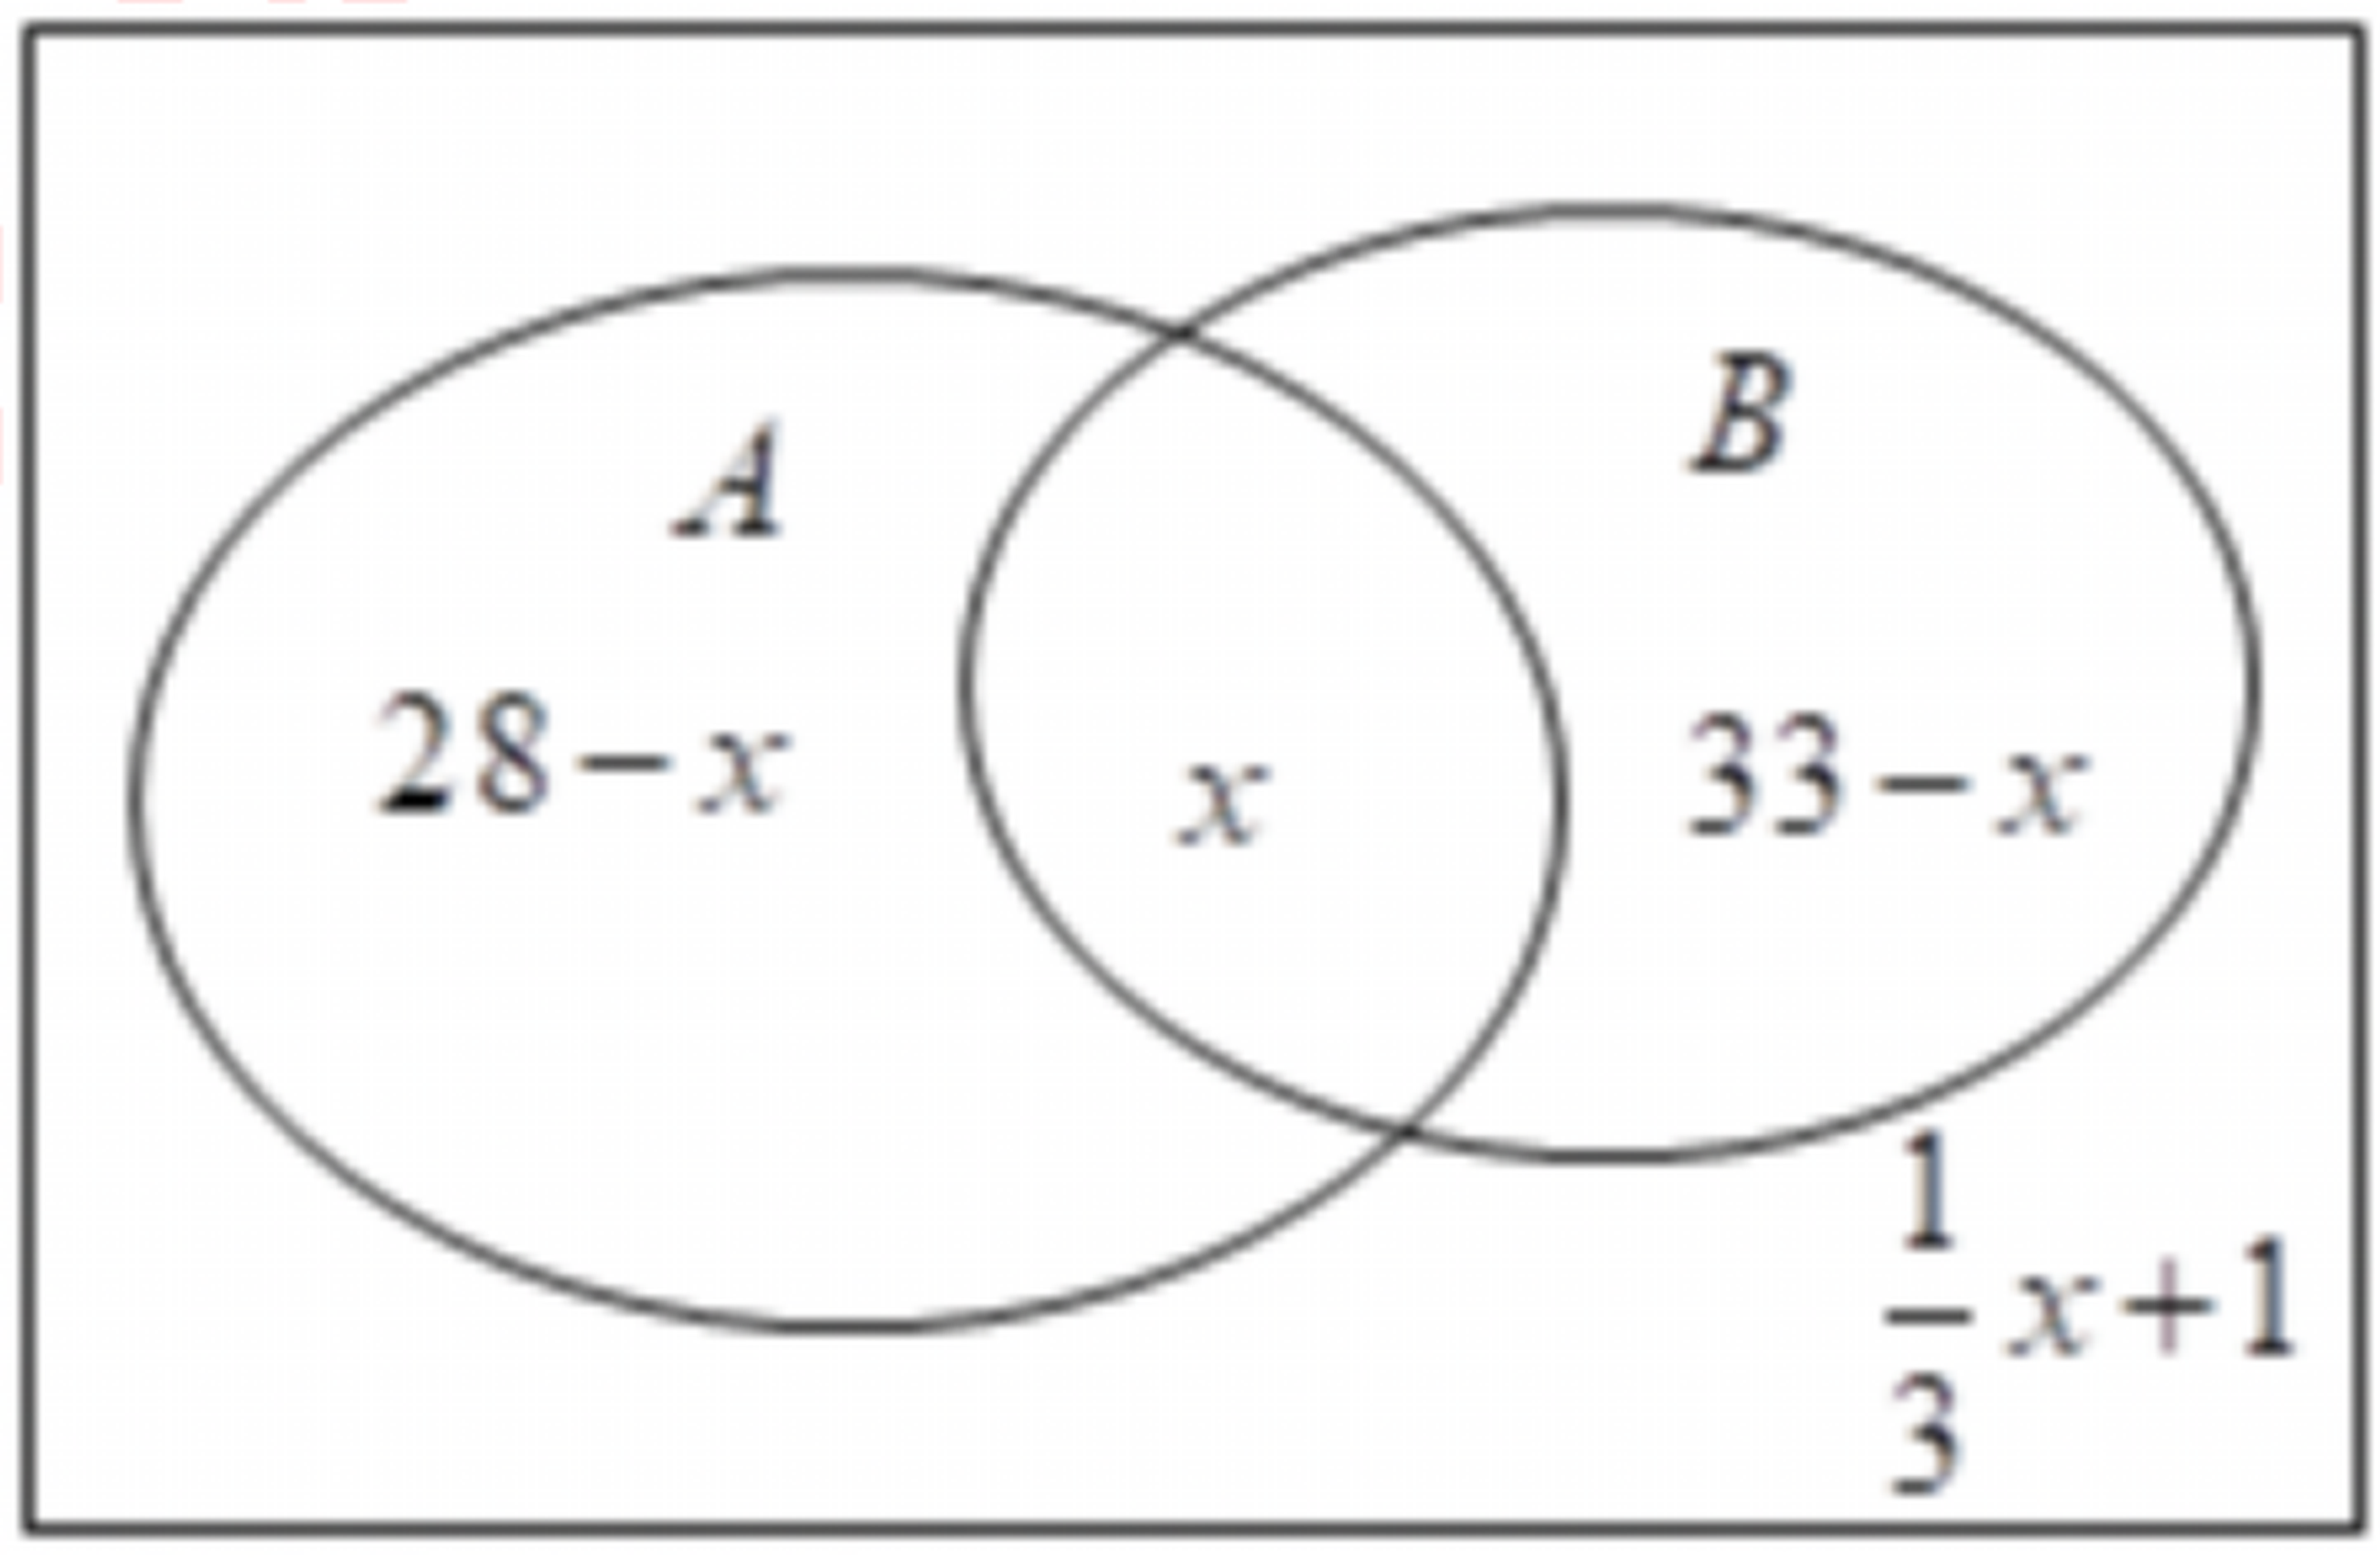
\includegraphics[width=0.42\textwidth]{figures/venn_AB_survey_50_x.png}
\end{center}
\step{则仅参加 $A$ 项的有 $(28-x)$ 人，仅参加 $B$ 项的有 $(33-x)$ 人，}
\step{$A$、$B$ 两项公益活动都不参加的有 $\left(\dfrac13x+1\right)$ 人，}
\step{由题意得 $x+(28-x)+(33-x)+\left(\dfrac13x+1\right)=50$，解得 $x=18$，}
\step{所以只参加 $A$ 项不参加 $B$ 项的有 $28-18=10$ 人.}
\solend
\fi

\item 设集合 $A=\{x\mid x^2-3x+2=0\}$，则满足 $A\cup B=\{0,1,2\}$ 的集合 $B$ 的个数是 \blankline[4.4em].

\ans{$4$}

\ifanswer
\solbegin
\step{$A=\{x\mid x^2-3x+2=0\}=\{x\mid x=1\text{ 或 }x=2\}=\{1,2\}$，}
\step{若 $A\cup B=\{0,1,2\}$，则 $0\in B$，}
\step{则 $B=\{0\},\{0,2\},\{1,0\},\{0,1,2\}$，共 $4$ 个.}
\solend
\fi

\item 已知全集 $U=\R$，集合 $A=\{x\mid x^2<4\}$，$B=\{y\mid y=x^2\}$，则图中阴影部分所表示的集合为 \blankline[4.4em].

\begin{center}
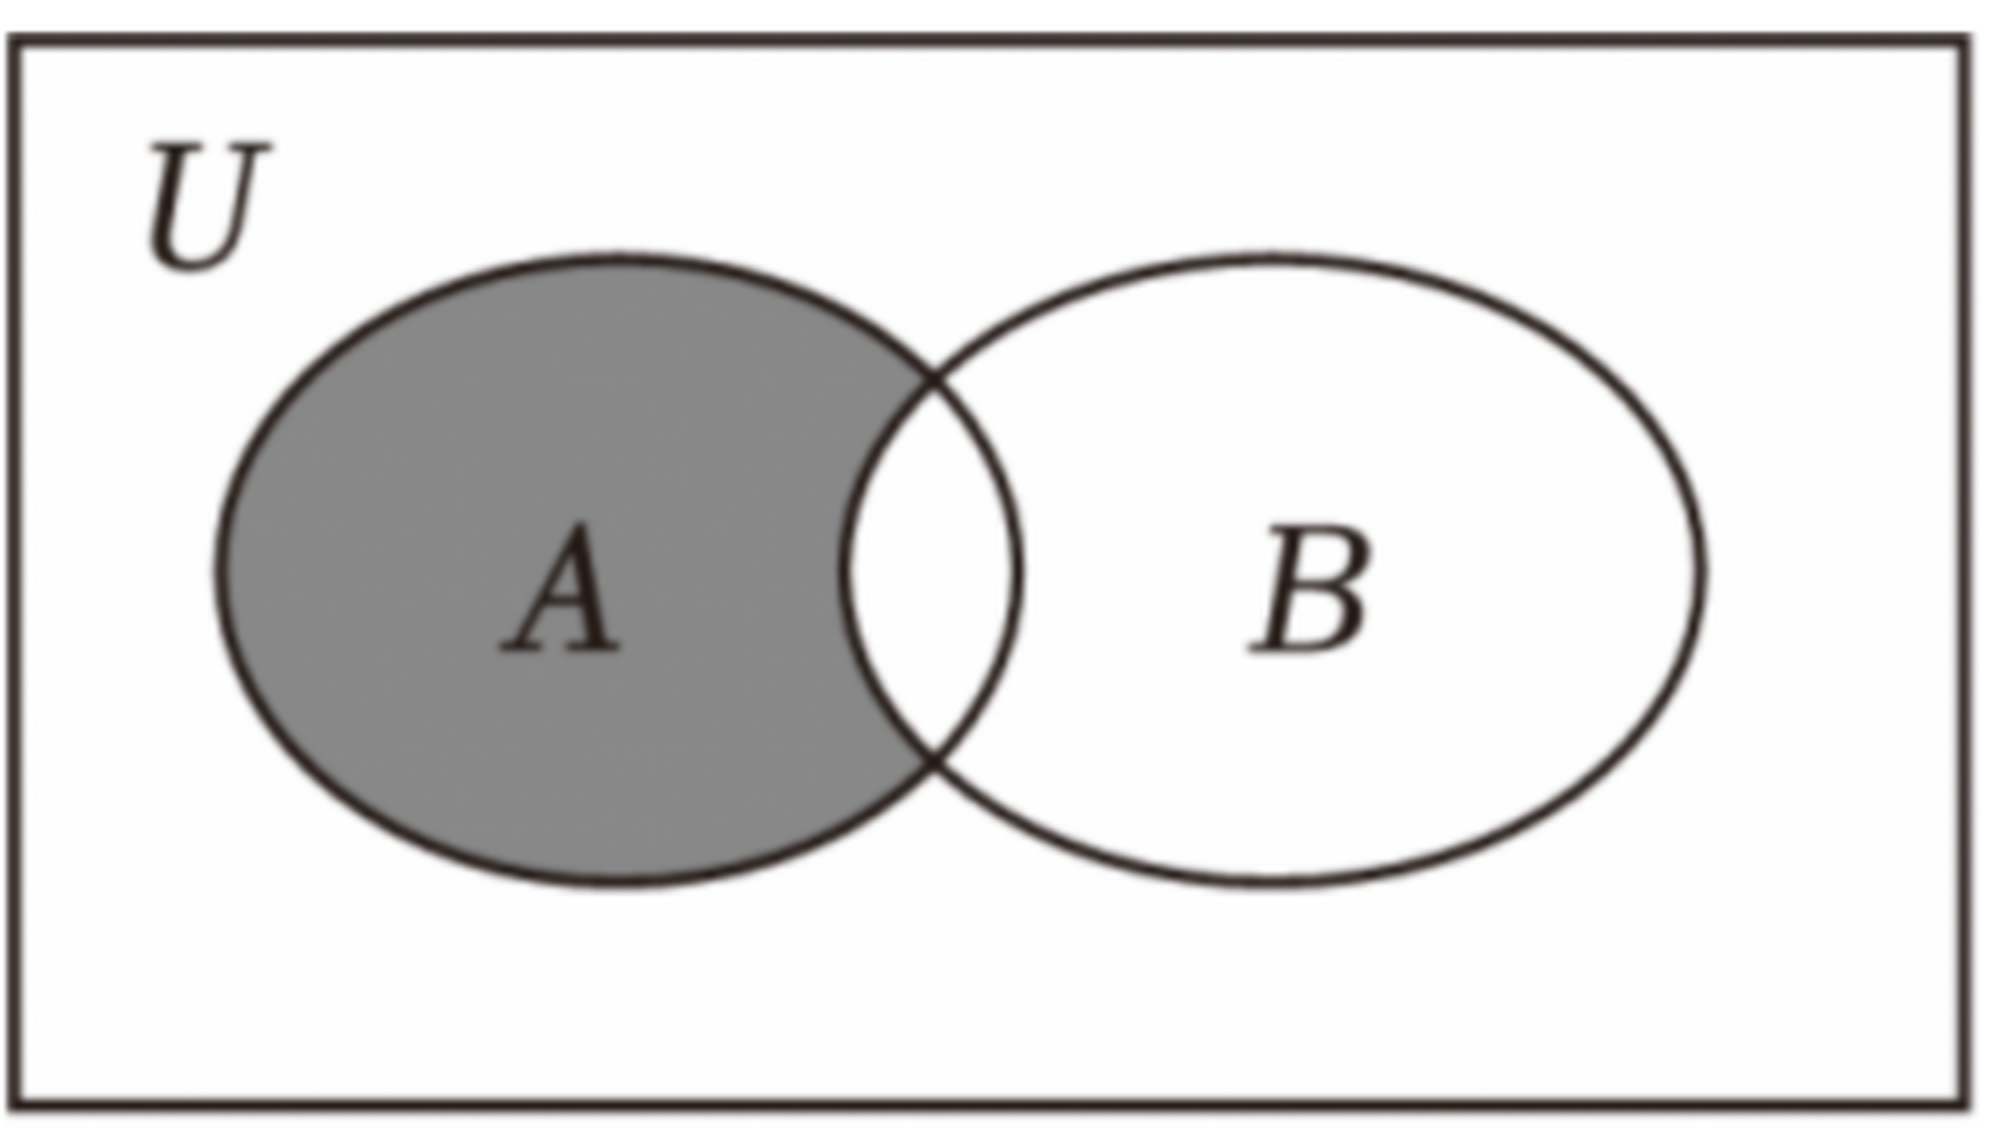
\includegraphics[width=0.34\textwidth]{figures/venn_A_shaded_U.png}
\end{center}

\ans{$A\cap\overline B=(-2,0)$}

\ifanswer
\solbegin
\step{集合 $A=\{x\mid x^2<4\}=(-2,2)$，$B=\{y\mid y=x^2\}=[0,+\infty)$，}
\step{图中阴影部分所表示的集合是 $A\cap\overline B=(-2,0)$.}
\solend
\fi

\item 如图所示，$M$、$P$、$S$ 是 $V$ 的三个子集，则阴影部分所表示的集合是 \blankline[5.4em].

\begin{center}
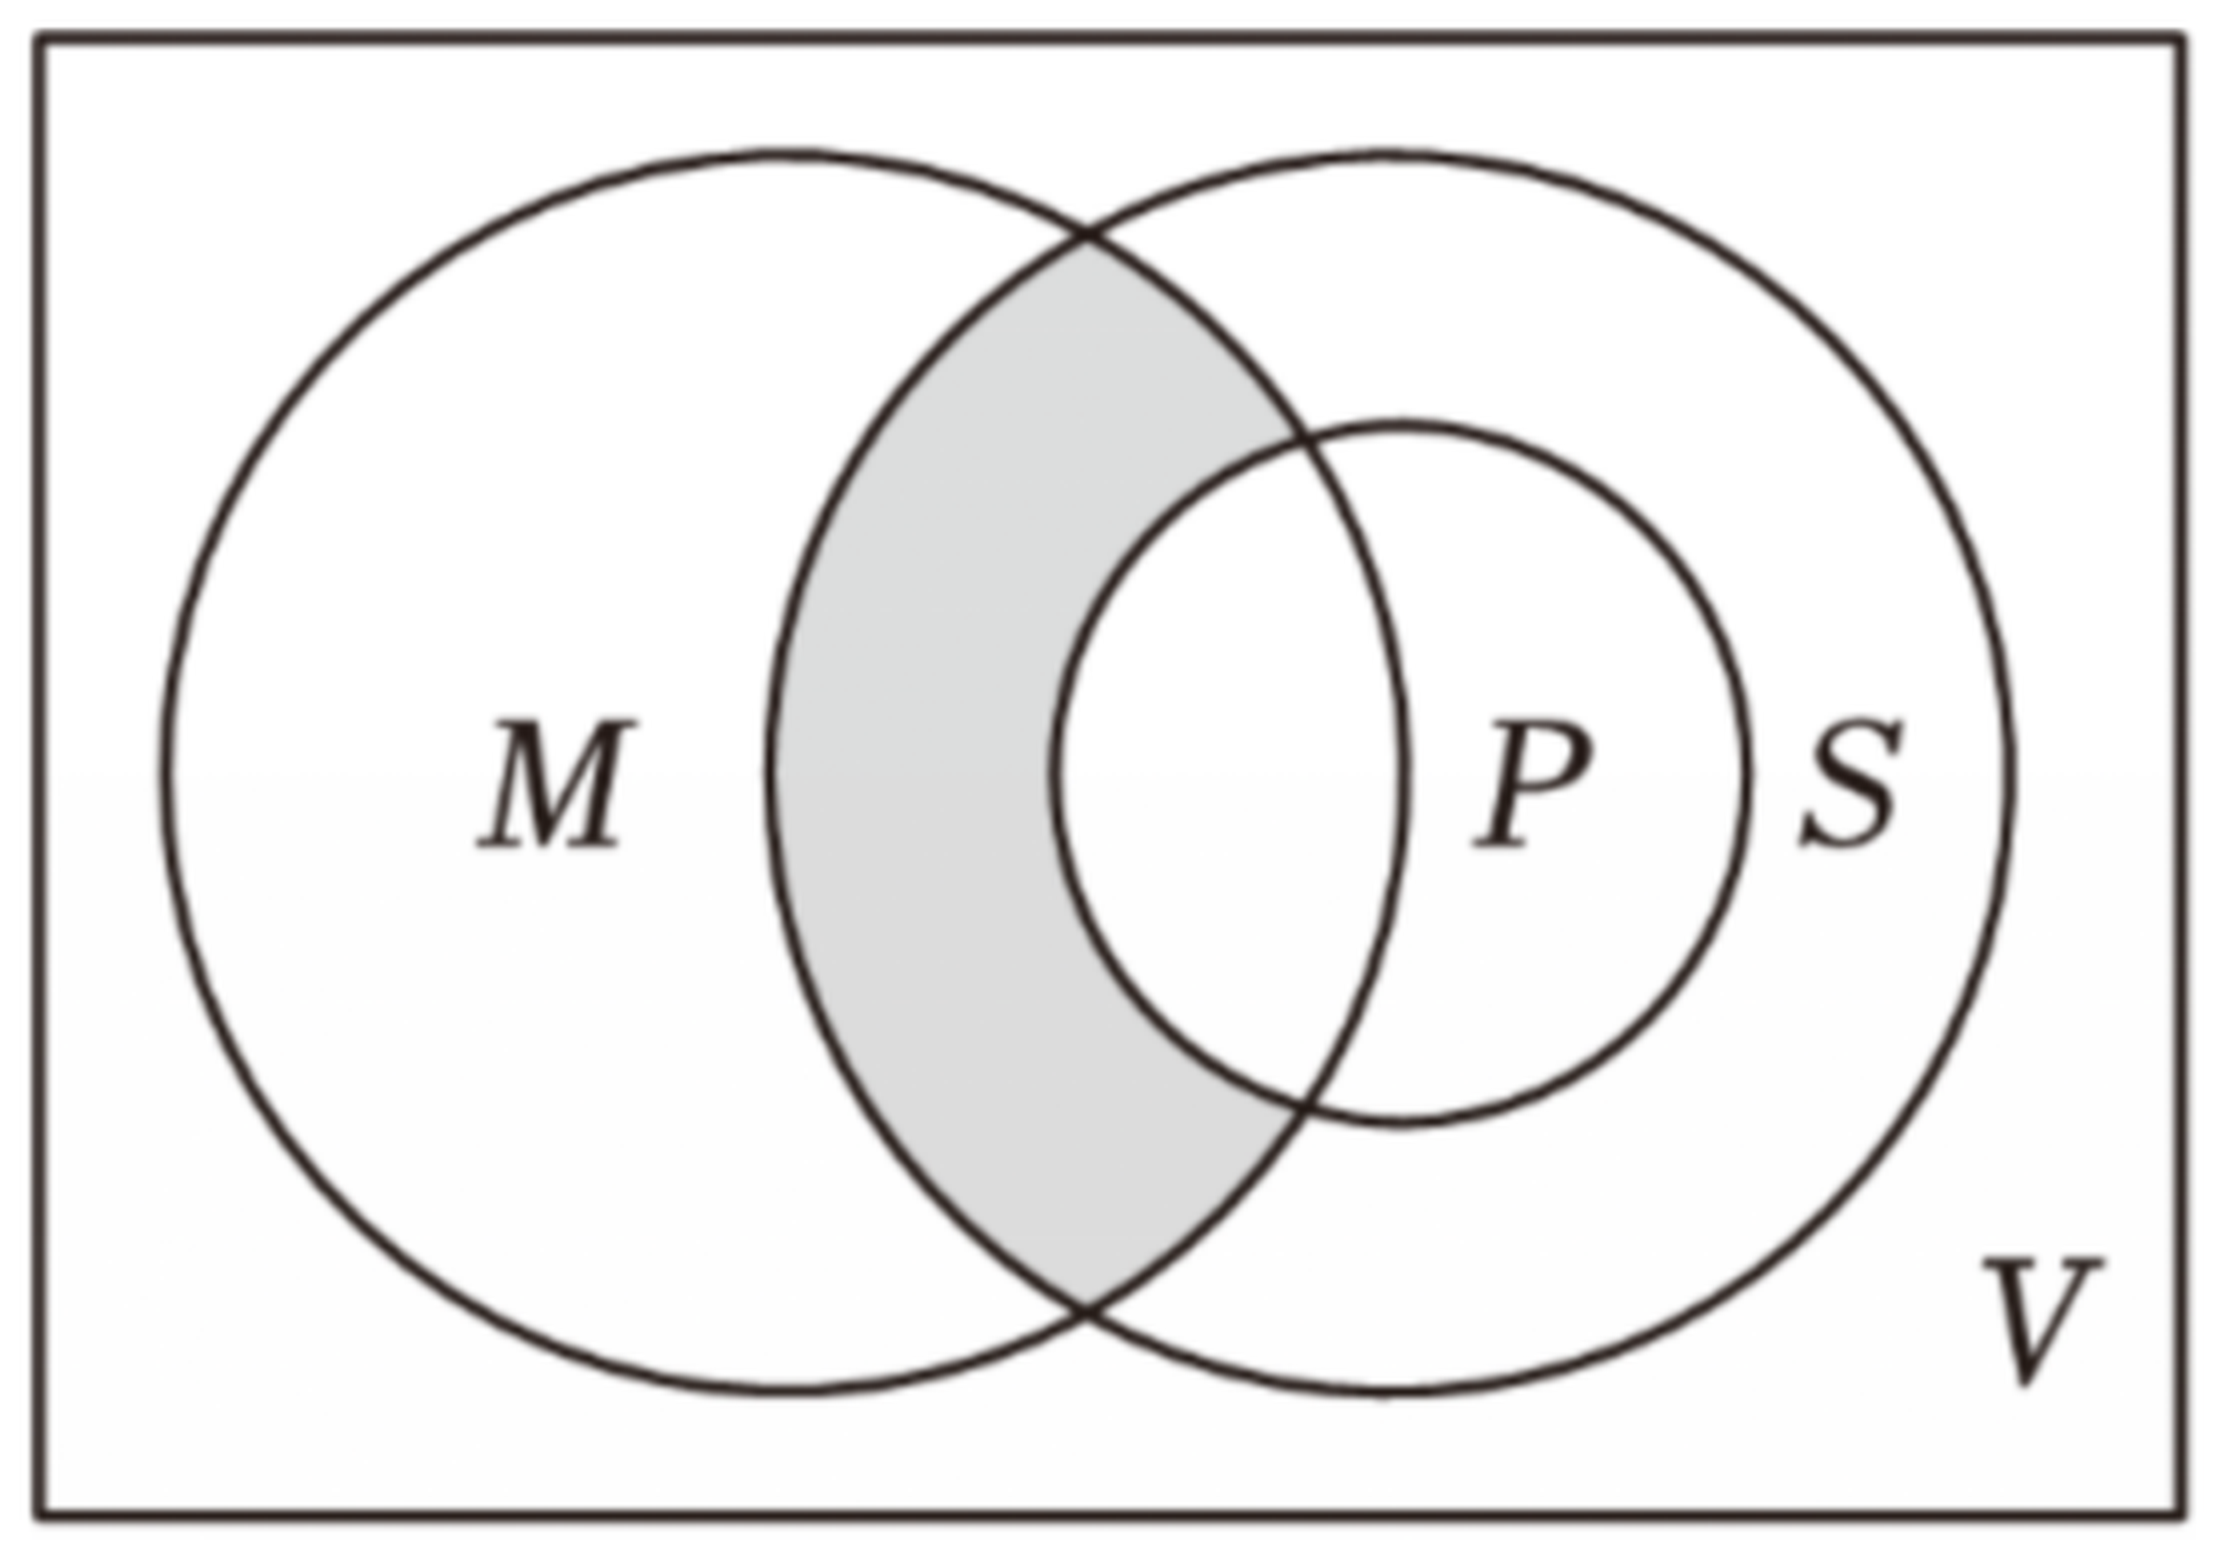
\includegraphics[width=0.38\textwidth]{figures/venn_MPS_V.png}
\end{center}

\ans{$(M\cap S)\cap(\complement_V P)$}

\item 下面六个关系式：① $\varnothing\subseteq\{a\}$；② $a\subseteq\{a\}$；③ $\{a\}\subseteq\{a\}$；④ $\{a\}\in\{a,b\}$；⑤ $a\in\{a,b,c\}$；⑥ $\varnothing\in\{a,b\}$；其中正确的是 \blankline[3.4em].

\ans{①③⑤}

\item 已知集合 $A=\{x\mid -1\le x\le a\}\ne\varnothing$，若 $\{y\mid y=x+1,x\in A\}=\{y\mid y=x^2,x\in A\}$，则实数 $a$ 值为 \blankline[4.4em].

\ans{$0$ 或 $\dfrac{1+\sqrt5}{2}$}

\ifanswer
\solbegin
\step{因为 $A=\{x\mid -1\le x\le a\}\ne\varnothing$，}
\step{所以 $\{y\mid y=x+1,x\in A\}=\{y\mid 0\le y\le a+1\}$，}
\step{$-1\le a\le1$ 时，$\{y\mid y=x^2,x\in A\}=\{y\mid 0\le y\le1\}$，}
\step{$a>1$ 时，$\{y\mid y=x^2,x\in A\}=\{y\mid 0\le y\le a^2\}$，}
\step{① $-1\le a\le1$ 时，$\{y\mid 0\le y\le a+1\}=\{y\mid 0\le y\le1\}$，则 $a+1=1$，解得 $a=0$；}
\step{② $a>1$ 时，$\{y\mid 0\le y\le a+1\}=\{y\mid 0\le y\le a^2\}$，则 $a^2=a+1$，解得 $a=\dfrac{1+\sqrt5}{2}$；}
\step{所以 $a=0$ 或 $\dfrac{1+\sqrt5}{2}$.}
\solend
\fi

\item 设集合 $A=\{(x,y)\mid x+y=22,x>0,y>0,x,y\text{ 均为质数}\}$ 的子集的个数为 \blankline[4.4em].

\ans{$32$}

\ifanswer
\solbegin
\step{集合 $A=\{(x,y)\mid x+y=22,x>0,y>0,x,y\text{ 均为质数}\}$}
\step{$=\{(3,19),(19,3),(5,17),(17,5),(11,11)\}$，则 $A$ 的子集的个数为 $2^5=32$.}
\solend
\fi

% 注：原卷本题题干印作「已知一个有四个数字元素的集合 $S$」；「数字元素」疑为「元素」之衍，
%     但原卷字形确为「数字」二字（已 3× 放大核对过），本稿照录，不代为改写。
\item 已知一个有四个数字元素的集合 $S$，$S$ 的所有子集的元素和（空集的元素和认为是 $0$）的总和为 $16192$，则 $S$ 的元素之和等于 \blankline[4.4em].

\ans{$2024$}

\ifanswer
\solbegin
\step{设 $S=\{a_1,a_2,a_3,a_4\}$，$S$ 的每个元素在所有子集中均出现 $2^3$ 次，}
\step{故 $(a_1+a_2+a_3+a_4)\cdot 2^3=16192$，所以 $a_1+a_2+a_3+a_4=2024$，}
\step{故 $S$ 的元素之和等于 $2024$.}
\solend
\fi

\item 设 $A$ 是非空数集，若对任意 $x$、$y\in A$，都有 $x+y\in A$、$xy\in A$，则称 $A$ 具有性质 $P$，给出以下命题：

①若 $A$ 具有性质 $P$，则 $A$ 可以是有限集；

②若 $A$ 具有性质 $P$，且 $A\ne\R$，则 $\overline A$ 具有性质 $P$；

③若 $A_1$、$A_2$ 具有性质 $P$，且 $A_1\cap A_2\ne\varnothing$，则 $A_1\cap A_2$ 具有性质 $P$；

④若 $A_1$、$A_2$ 具有性质 $P$，则 $A_1\cap A_2$ 具有性质 $P$.

其中所有真命题的序号是 \blankline[4.4em].

\ans{①③}

\ifanswer
\solbegin
\step{对于①，取集合 $A=\{0,1\}$ 具有性质 $P$，故 $A$ 可以是有限集，故①正确；}
\step{对于③，取 $x$、$y\in A_1\cap A_2$，则 $x\in A_1$，$x\in A_2$，$y\in A_1$，$y\in A_2$，}
\step{又 $A_1$、$A_2$ 具有性质 $P$，所以 $x+y\in A_1$，$xy\in A_1$，$x+y\in A_2$，$xy\in A_2$，}
\step{所以 $x+y\in A_1\cap A_2$，$xy\in A_1\cap A_2$，所以 $A_1\cap A_2$ 具有性质 $P$，故③正确；}
\step{对于④，取 $A_1=\{x\mid x=2k,k\in\Z\}$，$A_2=\{x\mid x=3k,k\in\Z\}$，$2\in A_1$，$3\in A_2$，}
\step{但 $2+3\notin A_1\cup A_2$，故④错误；}
\step{对于②，若 $A$ 具有性质 $P$，且 $A\ne\R$，假设 $\overline A$ 也具有性质 $P$，}
\step{设 $0\in A$，在 $\overline A$ 中任取一个 $x$，$x\ne0$，此时可证得 $-x\in A$，}
\step{否则若 $-x\in\overline A$，由于 $\overline A$ 也具有性质 $P$，则 $x+(-x)=0\in\overline A$，}
\step{与 $0\in A$ 矛盾，故 $-x\in A$，}
\step{由于 $A$ 具有性质 $P$，$\overline A$ 也具有性质 $P$，所以 $(-x)^2\in A$，$x^2\in\overline A$，}
\step{而 $(-x)^2=x^2$，这与 $A\cap\overline A=\varnothing$ 矛盾，}
\step{故当 $0\in A$ 且 $A$ 具有性质 $P$ 时，则 $\overline A$ 不具有性质 $P$，}
\step{同理当 $0\in\overline A$ 时，也可以类似推出矛盾，故②错误.}
\step{故正确的是①③.}
\solend
\fi

\item 已知 $S=\{1,2,3,4,5\}$，$A=\{1,2,5\}$，$T=\{t_1,t_2\}\subseteq S$，记 $A_1=\{x\mid x=a+t_1,a\in A,t_1\in T\}$，$A_2=\{x\mid x=b+t_2,b\in A,t_2\in T\}$，若 $A_1\cap A_2=\varnothing$，则集合 $T$ 为 \blankline[5.4em].

\ans{$T=\{1,3\}$ 或 $T=\{2,4\}$ 或 $T=\{3,5\}$}

\ifanswer
\solbegin
\step{若 $A_1\cap A_2=\varnothing$，即 $a+t_1\ne b+t_2$，则 $t_1-t_2\ne a-b$，其中 $a$、$b\in A$，}
\step{否则 $t_1+a=t_2+b$，$A_1\cap A_2\ne\varnothing$，}
\step{又 $S=\{1,2,3,4,5\}$，$A=\{1,2,5\}$，$T=\{t_1,t_2\}\subseteq S$，}
\step{$2-1=1$，$5-2=3$，$5-1=4$，则 $t_1$、$t_2$ 相差 $2$，}
\step{所以 $T=\{1,3\}$ 或 $T=\{2,4\}$ 或 $T=\{3,5\}$.}
\solend
\fi

\end{enumerate}

\bigsec{二、解答题}

\begin{enumerate}
\setcounter{enumi}{13}

\item 设集合 $P=\{1,2,3,m\}$，$Q=\{3,m^2\}$，且 $\overline P\cap Q=\varnothing$，求实数 $m$ 的值组成的集合.

\ans{$\{-1,0,\pm\sqrt2\}$}

\ansspace[5]

\ifanswer
\solbegin
\step{因为 $\overline P\cap Q=\varnothing$，所以 $Q\subseteq P$，所以 $m^2=1$ 或 $m^2=2$ 或 $m^2=m$，}
\step{考虑互异性，得 $m=-1$ 或 $m=\pm\sqrt2$ 或 $m=0$，}
\step{所以实数 $m$ 的值组成的集合为 $\{-1,0,\pm\sqrt2\}$.}
\solend
\fi

\item 若集合 $A=(-\infty,2]$，$B=\{x\mid kx+1<0,k\in\R\}$，$A\cap B=\varnothing$，求实数 $k$ 的取值范围.

\ans{$\left[-\dfrac12,0\right]$}

\ansspace[5]

\ifanswer
\solbegin
\step{若 $B=\varnothing$，则 $k=0$，符合题意，}
\step{若 $B\ne\varnothing$，当 $k>0$ 时，$B=\left(-\infty,-\dfrac1k\right)$，$A\cap B\ne\varnothing$，不合题意；}
\step{当 $k<0$ 时，$B=\left(-\dfrac1k,+\infty\right)$，由 $A\cap B=\varnothing$ 得 $-\dfrac1k\ge2$，即 $-\dfrac12\le k<0$，}
\step{故 $k$ 的取值范围是 $\left[-\dfrac12,0\right]$.}
\solend
\fi

\item 已知集合 $A=\{-4,2a-1,a^2\}$，$B=\{a-5,1-a,9\}$，分别求适合下列条件的 $a$ 的值.

% 两个小问不许与题干分家：试卷版第 2 页页末原本正好把 (1) 留在页底、(2) 翻到次页，
% 与 2026-09-15 修的三类难看切页同源，故在这里也加 \keepwithprev 守卫（三版都生效）。
\keepwithprev
（1）$9\in(A\cap B)$；

\keepwithprev
（2）$\{9\}=A\cap B$.

\ans{（1）$a=5$ 或 $a=-3$；（2）$a=-3$}

\ansspace[5]

\ifanswer
\solbegin
\stepm{（1）}{$9\in(A\cap B)$，所以 $9\in A$，}
\step{当 $2a-1=9$ 时，$a=5$，当 $a^2=9$ 时，即 $a=\pm3$，}
% 注：原卷此句结论印作「所以 $a$ 的值为 $5\backslash-3$」——「\」应是顿号之误，
%     本稿照录原卷字形（见文件头「原卷存疑」②）；按文意即 $a=5$ 或 $a=-3$。
\step{当 $a=3$ 时，$a-5=1-a$ 舍去，所以 $a$ 的值为 $5\backslash-3$.}
\stepm{（2）}{结合（1）的结论：}
\step{当 $2a-1=9$ 即 $a=5$ 时，$1-a=-4$，$\{9\}\ne(A\cap B)$，}
\step{当 $a^2=9$ 时，即 $a=\pm3$，当 $a=3$ 时，$a-5=1-a$ 舍去，}
\step{所以 $a$ 的值为 $-3$.}
\solend
\fi

\item 已知集合 $M=\{a,ab,a-b\}$，$N=\{0,|a|,b\}$，且 $M=N$，求实数 $a$、$b$ 的值.

\ans{$a=b=-1$}

\ansspace[5]

\ifanswer
\solbegin
\step{由集合元素的互异性，得 $a\ne0$，且 $b\ne0$，所以 $a-b=0$，即 $a=b$，}
\step{所以 $ab=|a|$，又由 $|a|\ne b=a$，得 $a<0$，故 $a=b=-1$.}
\solend
\fi

\item 已知集合 $A=\{x\mid -2<x<7\}$，$B=\{x\mid m+1\le x\le 2m-1\}$.

\keepwithprev
（1）当 $m=4$ 时，求 $A\cap B$、$A\cup B$；

\keepwithprev
（2）若 $A\cap B=B$，求实数 $m$ 的取值范围.

\ans{（1）$A\cap B=[5,7)$，$A\cup B=(-2,7]$；（2）$(-\infty,4)$}

\ansspace[5]

\ifanswer
\solbegin
\stepm{（1）}{当 $m=4$ 时，得集合 $A=\{x\mid -2<x<7\}$，$B=\{x\mid 5\le x\le7\}$，}
\step{得 $A\cap B=[5,7)$，$A\cup B=(-2,7]$.}
\stepm{（2）}{由 $A\cap B=B$ 得 $B\subseteq A$，}
\step{①当 $B=\varnothing$ 时，得 $m+1>2m-1$，解得 $m<2$；}
\step{②当 $B\ne\varnothing$ 时，得 $\begin{cases}m+1>-2\\ 2m-1<7\\ m+1\le2m-1\end{cases}$，解得 $2\le m<4$；}
\step{综上，实数 $m$ 的取值范围是 $(-\infty,4)$.}
\solend
\fi

\item 若集合 $A=\{x\mid x^2+5x-6=0\}$，$B=\{x\mid x^2+2(m+1)x+m^2-3=0\}$.

\keepwithprev
（1）当 $m=0$ 时，求集合 $A\cup B$；

\keepwithprev
（2）若 $A\cap B=B$，求实数 $m$ 的取值范围.

\ans{（1）$A\cup B=\{1,-6,-3\}$；（2）$\{m\mid m\le-2\}$}

\ansspace[5]

\ifanswer
\solbegin
\stepm{（1）}{由题意得，集合 $A=\{x\mid x^2+5x-6=0\}=\{1,-6\}$，}
\step{当 $m=0$ 时，$B=\{x\mid x^2+2x-3=0\}=\{1,-3\}$，}
\step{所以 $A\cup B=\{1,-6,-3\}$；}
\stepm{（2）}{由（1）得集合 $A=\{1,-6\}$，$B=\{x\mid x^2+2(m+1)x+m^2-3=0\}$，}
\step{若 $A\cap B=B$ 得 $B\subseteq A$，所以 $B=\varnothing$ 或 $\{-6\}$ 或 $\{1\}$ 或 $\{1,-6\}$，}
\step{当 $B=\varnothing$ 时，$\Delta=4(m+1)^2-4(m^2-3)<0$，解得 $m<-2$，}
\step{当 $B=\{-6\}$ 时，则 $\begin{cases}\Delta=4(m+1)^2-4(m^2-3)=0\\ 36-12(m+1)+m^2-3=0\end{cases}$，无解，}
\step{当 $B=\{1\}$ 时，则 $\begin{cases}\Delta=4(m+1)^2-4(m^2-3)=0\\ 1+2(m+1)+m^2-3=0\end{cases}$，解得 $m=-2$，}
\step{当 $B=\{1,-6\}$ 时，则 $\begin{cases}\Delta=4(m+1)^2-4(m^2-3)>0\\ 1+(-6)=-2(m+1)\\ 1\times(-6)=m^2-3\end{cases}$，无解，}
\step{综上所述，实数 $m$ 的取值范围为 $\{m\mid m\le-2\}$.}
\solend
\fi

% 压轴题：其后已无内容，故作答区全用可丢弃胶水（\ansspace*），并在题目前先量一下版面。
\ansneed{8cm}
\item 对于点集 $A=\{(x,y)\mid x=m,y=-3x+2,m\in\N,m\ge1\}$，$B=\{(x,y)\mid x=n,y=a(x^2-x+1),n\in\N,n\ge1\}$，是否存在非零整数 $a$，使得 $A\cap B\ne\varnothing$？

\ans{$a=-1$}

\ansspace*[10]

\ifanswer
\solbegin
\step{当 $A\cap B\ne\varnothing$ 时，$-3x+2=a(x^2-x+1)$，}
\step{$ax^2+(3-a)x+a-2=0$ ①有正整数解，}
\step{所以 $\Delta=(3-a)^2-4a(a-2)=-3a^2+2a+9$ 是平方数，}
\step{所以 $3a^2-2a-9\le0$，$\dfrac{1-2\sqrt7}{3}\le a\le\dfrac{1+2\sqrt7}{3}$，$a\ne0$，$a\in\Z$，}
\step{所以 $a=\pm1$ 或 $a=2$，}
\step{$a=-1$ 时 $\Delta=4$，这时①变为 $-x^2+4x-3=0$，解得 $x_1=1$，$x_2=3$，}
\step{$A\cap B=\{(1,-1),(3,-7)\}$.}
\step{$a=1$ 时 $\Delta=8$，不是平方数.}
\step{$a=2$ 时 $\Delta=1$，这时①变为 $2x^2+x=0$，没有正整数解.}
\step{所以 $a=-1$.}
\solend
\fi

\end{enumerate}

\end{document}
"
% 紧凑版：xelatex "\def\iscompact{1}% 高一19_延安中学_周末作业2.tex —— 高一上数学「2026-2027 年延安中学高一上周末作业 2」（试卷版/答案版）
% 试卷版：xelatex 高一19_延安中学_周末作业2.tex
% 答案版：xelatex "\def\isanswer{1}\input{高一19_延安中学_周末作业2.tex}"
% 紧凑版：xelatex "\def\iscompact{1}\input{高一19_延安中学_周末作业2.tex}"
%
% 原始材料是微信公众号图文（公众号「魔都数学加油站」，作者署名「破晓」，
% 原文链接 https://mp.weixin.qq.com/s/tHqWSV1StO5SHSXXQ4jeUA），正文为 6 张 PNG 页；
% 原文本身就是一份**讲评版**——题目下方直接印出【答案】或【解析】。本稿把答案与解析
% 移到答案版，试卷版即一张干净的空卷；试题文字、答案与解析均照原卷录入。
%
% 与原卷的排版差异（均已在 README「说明」中交代）：
%   ① 原文自**第 3 题**起（第 1、2 题未在该文发布），源码里以 \setcounter{enumi}{2} 起编；
%      全卷只有「一、填空题」「二、解答题」两节，无选择题；
%   ② 原卷本就印有两个分节标题（已在原图上逐页放大核对过），本稿照原卷分节，只把标题改排
%      成全稿统一的「大节标题」样式；
%   ③ 原卷的实数集、整数集、自然数集符号作正体 $R$、$Z$、$N$（第 15 题作粗体 $\mathbf{R}$，
%      第 20 题有 $N$ 与斜体 $Z$），本稿按全稿惯例统一写作 $\R$、$\Z$、$\N$；
%   ④ 第 4 题的韦恩图在原卷里印在【解析】右侧（题干并无「如图」二字），故本稿把该图放进
%      答案版的解析块内（`figures/venn_AB_survey_50_x.png`）；第 6、7 题的韦恩图是**题干图**
%      （题干作「图中阴影部分所表示的集合」），两版都排（`figures/venn_A_shaded_U.png`、
%      `figures/venn_MPS_V.png`）。三张图都取自原卷截图、4× LANCZOS 放大，不用 TikZ 手绘；
%   ⑤ 本卷也是「讲评版」，解析按全稿统一的 \solbegin/\step 分步重排（原卷为连续段落），
%      分步不改一字，只断句、断行；
%   ⑥ 标题前缀照**原卷**作「2026--2027 年…」（原卷标题即作「2026-2027年延安中学高一上周末
%      作业 2」）。同校的 高一06 作「学年度」——那是 高一02—高一09 那一批入库时统一改的；
%      后续入库的卷（高一10—高一17 与本卷）一律照原卷保留「年」，未强改，故同校两卷前缀不同。
%
% 原卷存疑两处（已逐处放大到能看清字形后核对，本稿照录并加注，见各题下的 `%` 注）：
%   （另有第三处「第 12 题【解析】末句」原先记作存疑，2026-09-26 第二轮核对放大后发现
%     原卷印的是「$0\in\overline A$」——A 上确有横杠，是本稿当初漏抄了 $\overline{}$；
%     已按原卷补回，故该条从存疑清单里删去，不计为原卷问题。）
%   ① 第 11 题题干印作「已知一个有四个数字元素的集合 $S$」，「数字元素」疑为「元素」之衍；
%   ② 第 16 题 (1) 结论印作「$a$ 的值为 $5\backslash-3$」，其中的「\」应是顿号之误
%      （由 (2) 的结论「$a$ 的值为 $-3$」可反推，(1) 的答案是 $5$ 或 $-3$）；

% 本篇在公众号「魔都数学加油站」连载里的编号是「27学年高一19」，本地编号与之对齐（高一19）；
% 对应关系见 README「与公众号连载号的对照表」。
\documentclass[a4paper,11pt]{article}
\usepackage{common}

\begin{document}

\examtitlest{2026--2027 年延安中学高一上周末作业 2}{集合与常用逻辑用语}

\bigsec{一、填空题}

\begin{enumerate}
% 原卷填空题从第 3 题起（1、2 未在该文中发布），须与解答题的 \setcounter{enumi}{13} 对齐
\setcounter{enumi}{2}
\item 已知全集 $U=\{1,2,3,4,5\}$，$M=\{1,2\}$，$P=\{1,3,5\}$，则 $M\cap\overline P=$ \blankline[4.4em].

\ans{$\{2\}$}

\item 某公司共有 $50$ 人，此次组织参加社会公益活动，其中参加 $A$ 项公益活动的有 $28$ 人，参加 $B$ 项公益活动的有 $33$ 人，且 $A$、$B$ 两项公益活动都不参加的人数比都参加的人数的三分之一多 $1$ 人，则只参加 $A$ 项不参加 $B$ 项的人数是 \blankline[4.4em].

\ans{$10$}

\ifanswer
\solbegin
\step{如图所示，设 $A$、$B$ 两项公益活动都参加的有 $x$ 人，}
\begin{center}
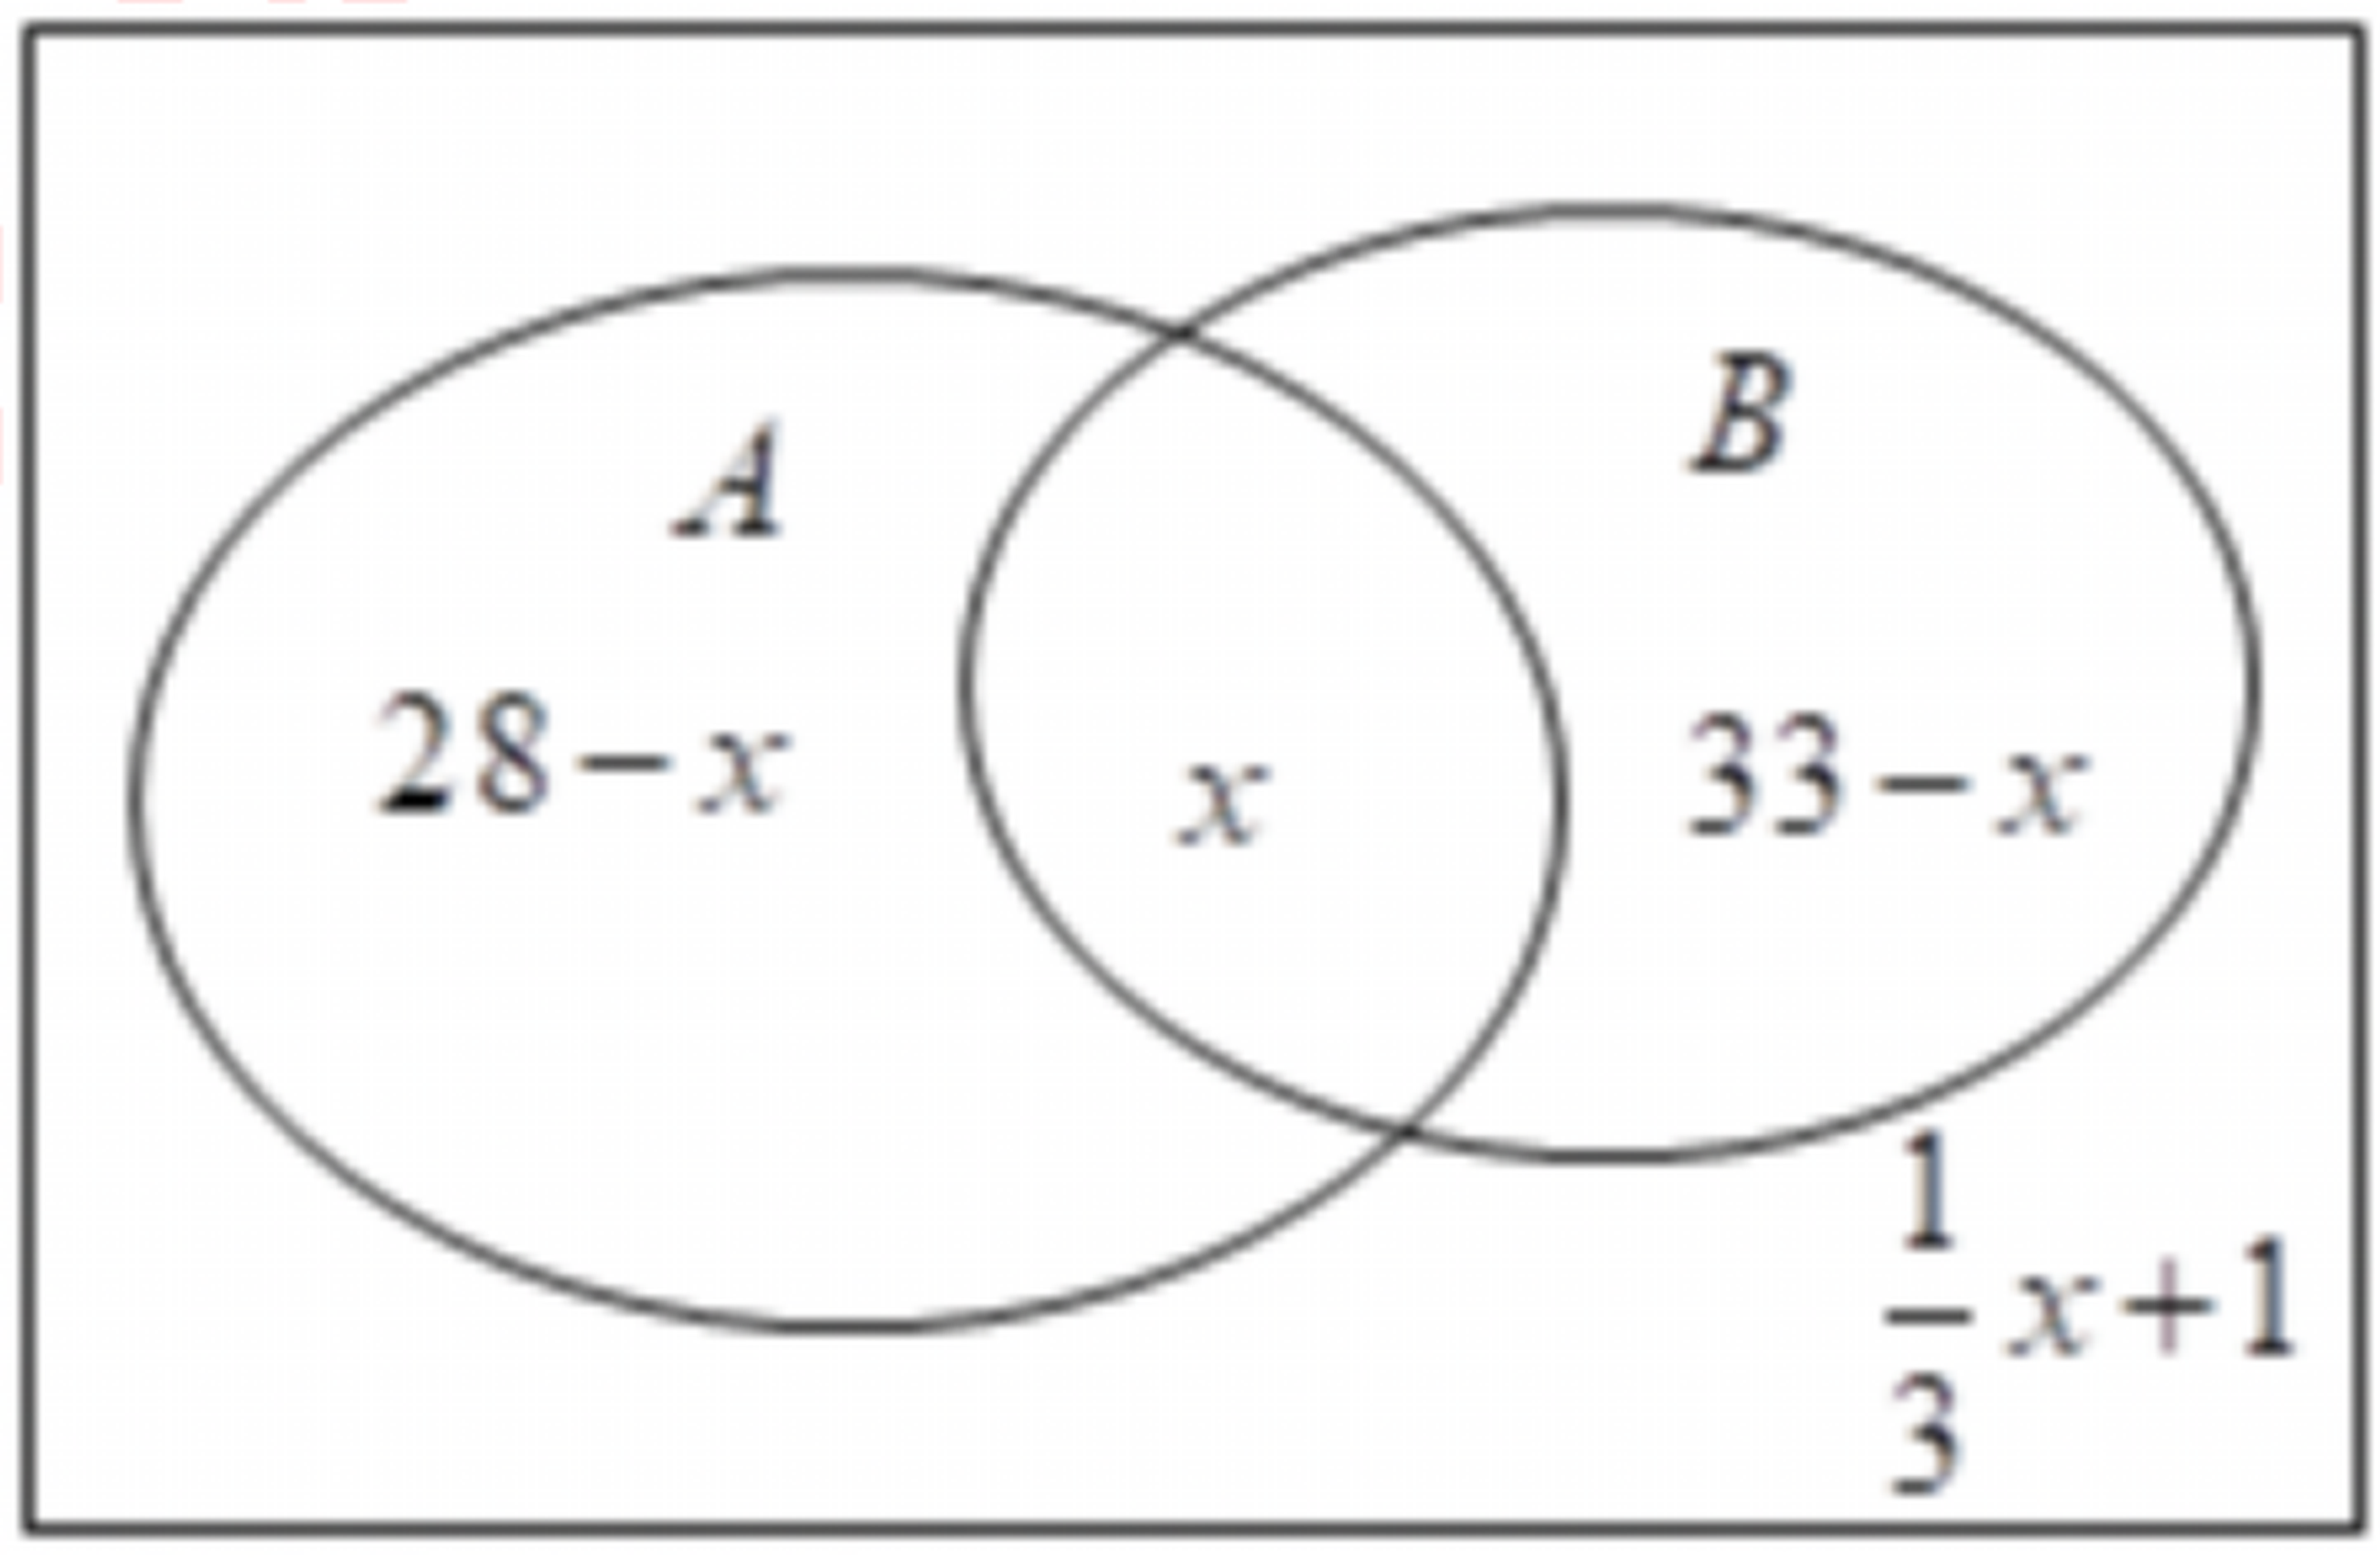
\includegraphics[width=0.42\textwidth]{figures/venn_AB_survey_50_x.png}
\end{center}
\step{则仅参加 $A$ 项的有 $(28-x)$ 人，仅参加 $B$ 项的有 $(33-x)$ 人，}
\step{$A$、$B$ 两项公益活动都不参加的有 $\left(\dfrac13x+1\right)$ 人，}
\step{由题意得 $x+(28-x)+(33-x)+\left(\dfrac13x+1\right)=50$，解得 $x=18$，}
\step{所以只参加 $A$ 项不参加 $B$ 项的有 $28-18=10$ 人.}
\solend
\fi

\item 设集合 $A=\{x\mid x^2-3x+2=0\}$，则满足 $A\cup B=\{0,1,2\}$ 的集合 $B$ 的个数是 \blankline[4.4em].

\ans{$4$}

\ifanswer
\solbegin
\step{$A=\{x\mid x^2-3x+2=0\}=\{x\mid x=1\text{ 或 }x=2\}=\{1,2\}$，}
\step{若 $A\cup B=\{0,1,2\}$，则 $0\in B$，}
\step{则 $B=\{0\},\{0,2\},\{1,0\},\{0,1,2\}$，共 $4$ 个.}
\solend
\fi

\item 已知全集 $U=\R$，集合 $A=\{x\mid x^2<4\}$，$B=\{y\mid y=x^2\}$，则图中阴影部分所表示的集合为 \blankline[4.4em].

\begin{center}
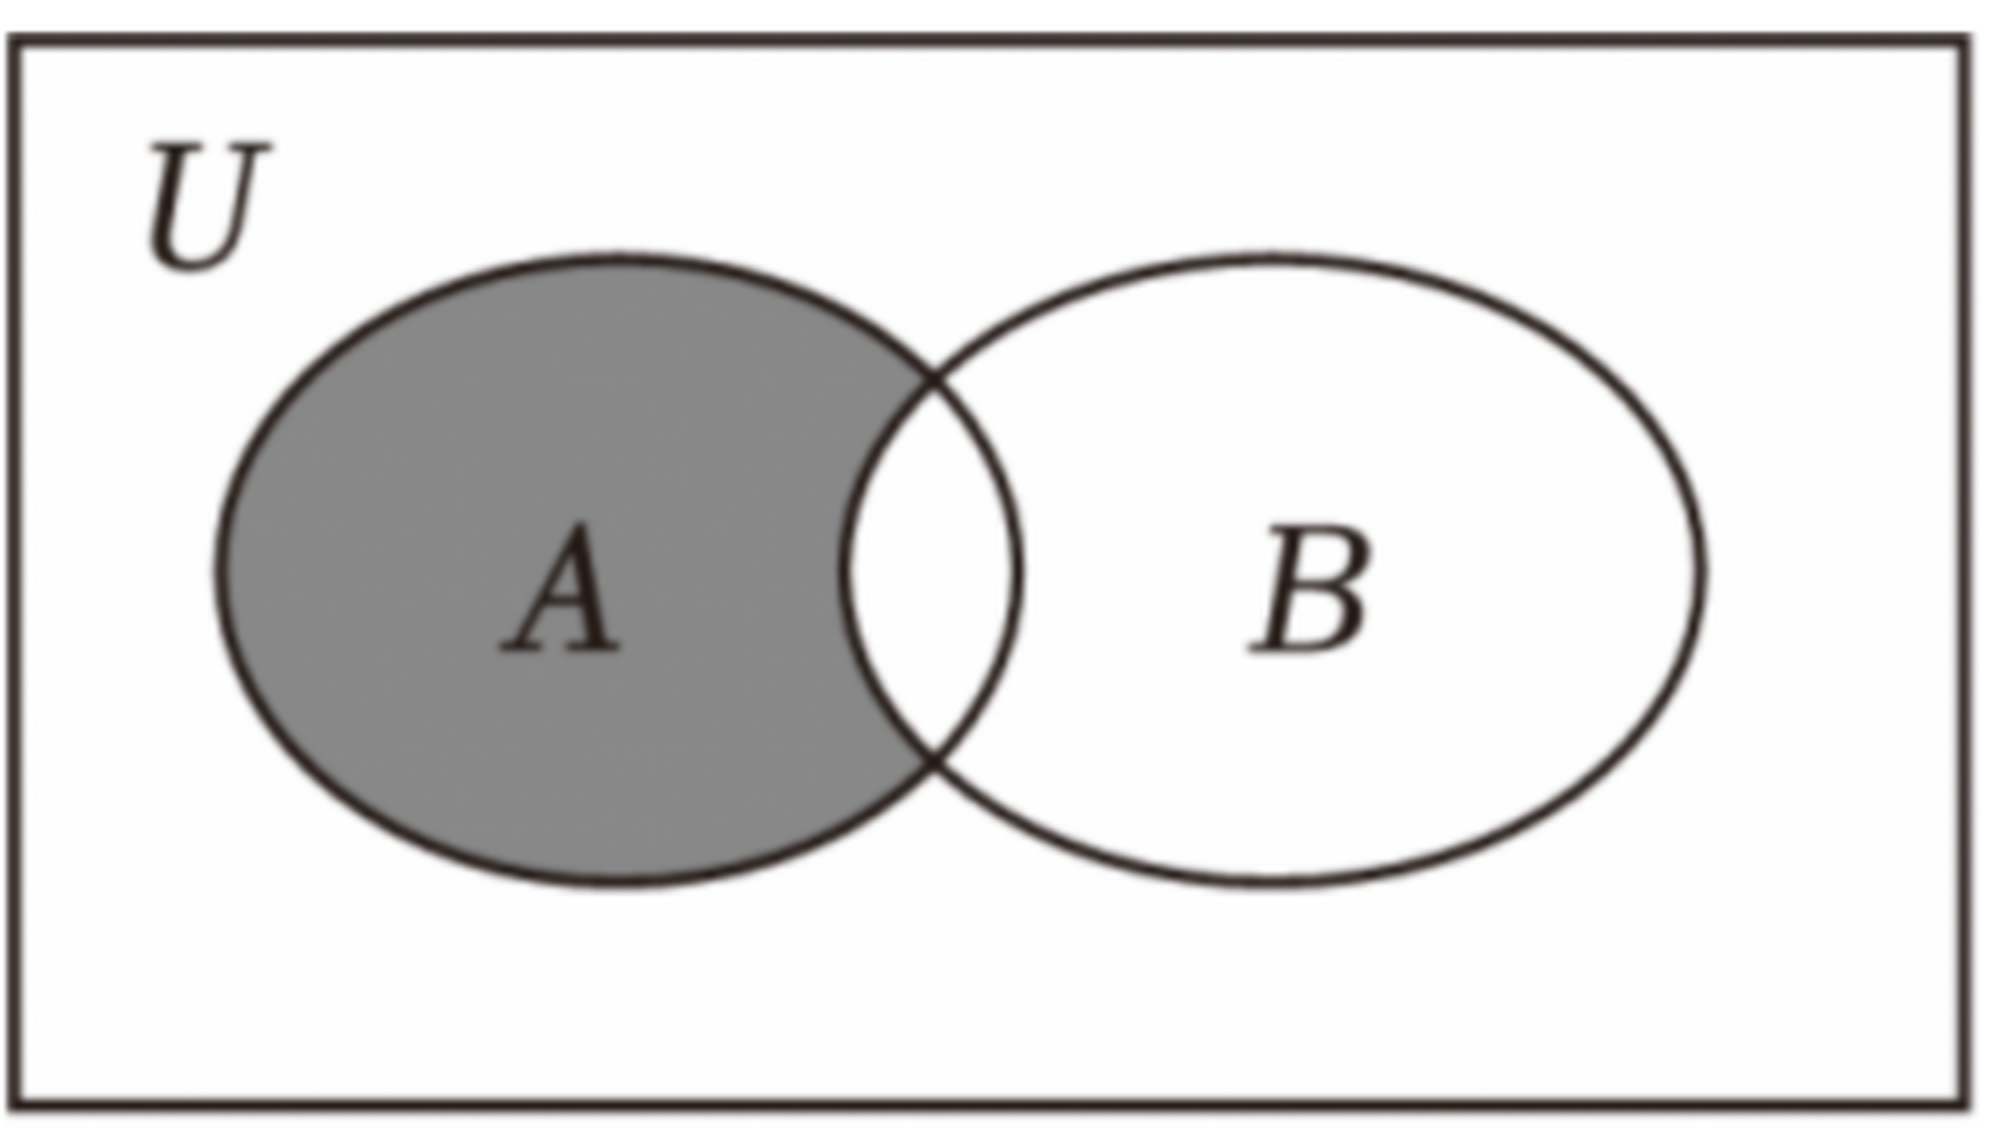
\includegraphics[width=0.34\textwidth]{figures/venn_A_shaded_U.png}
\end{center}

\ans{$A\cap\overline B=(-2,0)$}

\ifanswer
\solbegin
\step{集合 $A=\{x\mid x^2<4\}=(-2,2)$，$B=\{y\mid y=x^2\}=[0,+\infty)$，}
\step{图中阴影部分所表示的集合是 $A\cap\overline B=(-2,0)$.}
\solend
\fi

\item 如图所示，$M$、$P$、$S$ 是 $V$ 的三个子集，则阴影部分所表示的集合是 \blankline[5.4em].

\begin{center}
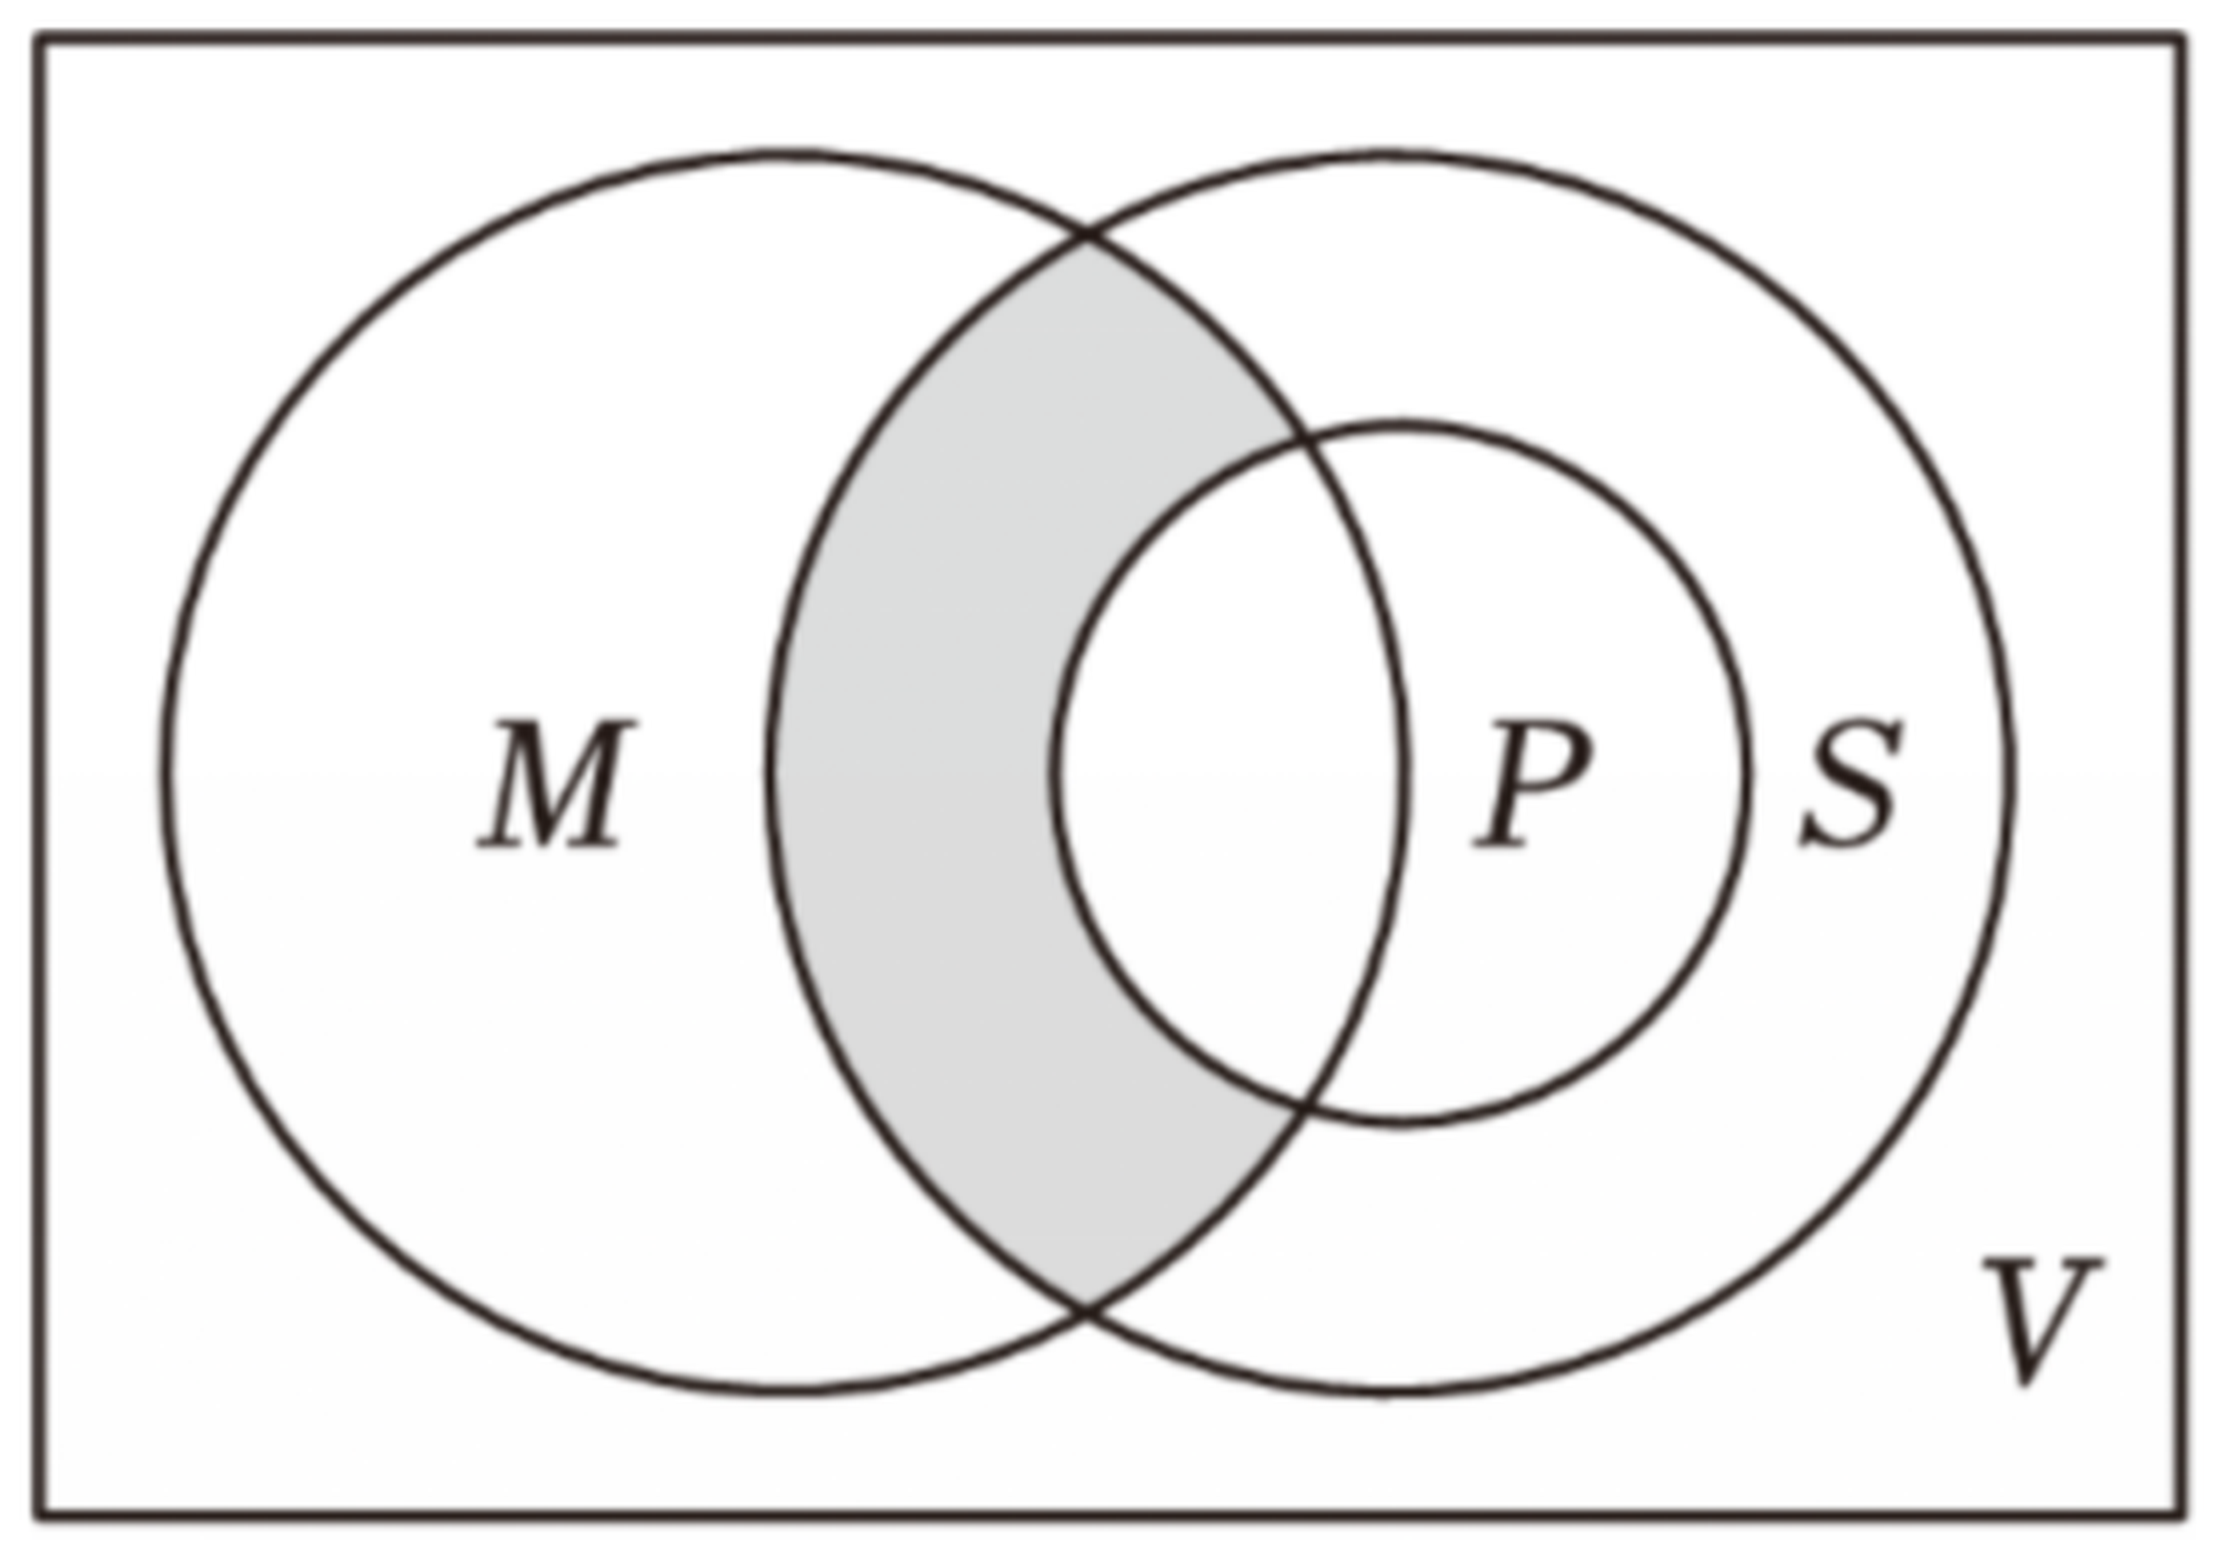
\includegraphics[width=0.38\textwidth]{figures/venn_MPS_V.png}
\end{center}

\ans{$(M\cap S)\cap(\complement_V P)$}

\item 下面六个关系式：① $\varnothing\subseteq\{a\}$；② $a\subseteq\{a\}$；③ $\{a\}\subseteq\{a\}$；④ $\{a\}\in\{a,b\}$；⑤ $a\in\{a,b,c\}$；⑥ $\varnothing\in\{a,b\}$；其中正确的是 \blankline[3.4em].

\ans{①③⑤}

\item 已知集合 $A=\{x\mid -1\le x\le a\}\ne\varnothing$，若 $\{y\mid y=x+1,x\in A\}=\{y\mid y=x^2,x\in A\}$，则实数 $a$ 值为 \blankline[4.4em].

\ans{$0$ 或 $\dfrac{1+\sqrt5}{2}$}

\ifanswer
\solbegin
\step{因为 $A=\{x\mid -1\le x\le a\}\ne\varnothing$，}
\step{所以 $\{y\mid y=x+1,x\in A\}=\{y\mid 0\le y\le a+1\}$，}
\step{$-1\le a\le1$ 时，$\{y\mid y=x^2,x\in A\}=\{y\mid 0\le y\le1\}$，}
\step{$a>1$ 时，$\{y\mid y=x^2,x\in A\}=\{y\mid 0\le y\le a^2\}$，}
\step{① $-1\le a\le1$ 时，$\{y\mid 0\le y\le a+1\}=\{y\mid 0\le y\le1\}$，则 $a+1=1$，解得 $a=0$；}
\step{② $a>1$ 时，$\{y\mid 0\le y\le a+1\}=\{y\mid 0\le y\le a^2\}$，则 $a^2=a+1$，解得 $a=\dfrac{1+\sqrt5}{2}$；}
\step{所以 $a=0$ 或 $\dfrac{1+\sqrt5}{2}$.}
\solend
\fi

\item 设集合 $A=\{(x,y)\mid x+y=22,x>0,y>0,x,y\text{ 均为质数}\}$ 的子集的个数为 \blankline[4.4em].

\ans{$32$}

\ifanswer
\solbegin
\step{集合 $A=\{(x,y)\mid x+y=22,x>0,y>0,x,y\text{ 均为质数}\}$}
\step{$=\{(3,19),(19,3),(5,17),(17,5),(11,11)\}$，则 $A$ 的子集的个数为 $2^5=32$.}
\solend
\fi

% 注：原卷本题题干印作「已知一个有四个数字元素的集合 $S$」；「数字元素」疑为「元素」之衍，
%     但原卷字形确为「数字」二字（已 3× 放大核对过），本稿照录，不代为改写。
\item 已知一个有四个数字元素的集合 $S$，$S$ 的所有子集的元素和（空集的元素和认为是 $0$）的总和为 $16192$，则 $S$ 的元素之和等于 \blankline[4.4em].

\ans{$2024$}

\ifanswer
\solbegin
\step{设 $S=\{a_1,a_2,a_3,a_4\}$，$S$ 的每个元素在所有子集中均出现 $2^3$ 次，}
\step{故 $(a_1+a_2+a_3+a_4)\cdot 2^3=16192$，所以 $a_1+a_2+a_3+a_4=2024$，}
\step{故 $S$ 的元素之和等于 $2024$.}
\solend
\fi

\item 设 $A$ 是非空数集，若对任意 $x$、$y\in A$，都有 $x+y\in A$、$xy\in A$，则称 $A$ 具有性质 $P$，给出以下命题：

①若 $A$ 具有性质 $P$，则 $A$ 可以是有限集；

②若 $A$ 具有性质 $P$，且 $A\ne\R$，则 $\overline A$ 具有性质 $P$；

③若 $A_1$、$A_2$ 具有性质 $P$，且 $A_1\cap A_2\ne\varnothing$，则 $A_1\cap A_2$ 具有性质 $P$；

④若 $A_1$、$A_2$ 具有性质 $P$，则 $A_1\cap A_2$ 具有性质 $P$.

其中所有真命题的序号是 \blankline[4.4em].

\ans{①③}

\ifanswer
\solbegin
\step{对于①，取集合 $A=\{0,1\}$ 具有性质 $P$，故 $A$ 可以是有限集，故①正确；}
\step{对于③，取 $x$、$y\in A_1\cap A_2$，则 $x\in A_1$，$x\in A_2$，$y\in A_1$，$y\in A_2$，}
\step{又 $A_1$、$A_2$ 具有性质 $P$，所以 $x+y\in A_1$，$xy\in A_1$，$x+y\in A_2$，$xy\in A_2$，}
\step{所以 $x+y\in A_1\cap A_2$，$xy\in A_1\cap A_2$，所以 $A_1\cap A_2$ 具有性质 $P$，故③正确；}
\step{对于④，取 $A_1=\{x\mid x=2k,k\in\Z\}$，$A_2=\{x\mid x=3k,k\in\Z\}$，$2\in A_1$，$3\in A_2$，}
\step{但 $2+3\notin A_1\cup A_2$，故④错误；}
\step{对于②，若 $A$ 具有性质 $P$，且 $A\ne\R$，假设 $\overline A$ 也具有性质 $P$，}
\step{设 $0\in A$，在 $\overline A$ 中任取一个 $x$，$x\ne0$，此时可证得 $-x\in A$，}
\step{否则若 $-x\in\overline A$，由于 $\overline A$ 也具有性质 $P$，则 $x+(-x)=0\in\overline A$，}
\step{与 $0\in A$ 矛盾，故 $-x\in A$，}
\step{由于 $A$ 具有性质 $P$，$\overline A$ 也具有性质 $P$，所以 $(-x)^2\in A$，$x^2\in\overline A$，}
\step{而 $(-x)^2=x^2$，这与 $A\cap\overline A=\varnothing$ 矛盾，}
\step{故当 $0\in A$ 且 $A$ 具有性质 $P$ 时，则 $\overline A$ 不具有性质 $P$，}
\step{同理当 $0\in\overline A$ 时，也可以类似推出矛盾，故②错误.}
\step{故正确的是①③.}
\solend
\fi

\item 已知 $S=\{1,2,3,4,5\}$，$A=\{1,2,5\}$，$T=\{t_1,t_2\}\subseteq S$，记 $A_1=\{x\mid x=a+t_1,a\in A,t_1\in T\}$，$A_2=\{x\mid x=b+t_2,b\in A,t_2\in T\}$，若 $A_1\cap A_2=\varnothing$，则集合 $T$ 为 \blankline[5.4em].

\ans{$T=\{1,3\}$ 或 $T=\{2,4\}$ 或 $T=\{3,5\}$}

\ifanswer
\solbegin
\step{若 $A_1\cap A_2=\varnothing$，即 $a+t_1\ne b+t_2$，则 $t_1-t_2\ne a-b$，其中 $a$、$b\in A$，}
\step{否则 $t_1+a=t_2+b$，$A_1\cap A_2\ne\varnothing$，}
\step{又 $S=\{1,2,3,4,5\}$，$A=\{1,2,5\}$，$T=\{t_1,t_2\}\subseteq S$，}
\step{$2-1=1$，$5-2=3$，$5-1=4$，则 $t_1$、$t_2$ 相差 $2$，}
\step{所以 $T=\{1,3\}$ 或 $T=\{2,4\}$ 或 $T=\{3,5\}$.}
\solend
\fi

\end{enumerate}

\bigsec{二、解答题}

\begin{enumerate}
\setcounter{enumi}{13}

\item 设集合 $P=\{1,2,3,m\}$，$Q=\{3,m^2\}$，且 $\overline P\cap Q=\varnothing$，求实数 $m$ 的值组成的集合.

\ans{$\{-1,0,\pm\sqrt2\}$}

\ansspace[5]

\ifanswer
\solbegin
\step{因为 $\overline P\cap Q=\varnothing$，所以 $Q\subseteq P$，所以 $m^2=1$ 或 $m^2=2$ 或 $m^2=m$，}
\step{考虑互异性，得 $m=-1$ 或 $m=\pm\sqrt2$ 或 $m=0$，}
\step{所以实数 $m$ 的值组成的集合为 $\{-1,0,\pm\sqrt2\}$.}
\solend
\fi

\item 若集合 $A=(-\infty,2]$，$B=\{x\mid kx+1<0,k\in\R\}$，$A\cap B=\varnothing$，求实数 $k$ 的取值范围.

\ans{$\left[-\dfrac12,0\right]$}

\ansspace[5]

\ifanswer
\solbegin
\step{若 $B=\varnothing$，则 $k=0$，符合题意，}
\step{若 $B\ne\varnothing$，当 $k>0$ 时，$B=\left(-\infty,-\dfrac1k\right)$，$A\cap B\ne\varnothing$，不合题意；}
\step{当 $k<0$ 时，$B=\left(-\dfrac1k,+\infty\right)$，由 $A\cap B=\varnothing$ 得 $-\dfrac1k\ge2$，即 $-\dfrac12\le k<0$，}
\step{故 $k$ 的取值范围是 $\left[-\dfrac12,0\right]$.}
\solend
\fi

\item 已知集合 $A=\{-4,2a-1,a^2\}$，$B=\{a-5,1-a,9\}$，分别求适合下列条件的 $a$ 的值.

% 两个小问不许与题干分家：试卷版第 2 页页末原本正好把 (1) 留在页底、(2) 翻到次页，
% 与 2026-09-15 修的三类难看切页同源，故在这里也加 \keepwithprev 守卫（三版都生效）。
\keepwithprev
（1）$9\in(A\cap B)$；

\keepwithprev
（2）$\{9\}=A\cap B$.

\ans{（1）$a=5$ 或 $a=-3$；（2）$a=-3$}

\ansspace[5]

\ifanswer
\solbegin
\stepm{（1）}{$9\in(A\cap B)$，所以 $9\in A$，}
\step{当 $2a-1=9$ 时，$a=5$，当 $a^2=9$ 时，即 $a=\pm3$，}
% 注：原卷此句结论印作「所以 $a$ 的值为 $5\backslash-3$」——「\」应是顿号之误，
%     本稿照录原卷字形（见文件头「原卷存疑」②）；按文意即 $a=5$ 或 $a=-3$。
\step{当 $a=3$ 时，$a-5=1-a$ 舍去，所以 $a$ 的值为 $5\backslash-3$.}
\stepm{（2）}{结合（1）的结论：}
\step{当 $2a-1=9$ 即 $a=5$ 时，$1-a=-4$，$\{9\}\ne(A\cap B)$，}
\step{当 $a^2=9$ 时，即 $a=\pm3$，当 $a=3$ 时，$a-5=1-a$ 舍去，}
\step{所以 $a$ 的值为 $-3$.}
\solend
\fi

\item 已知集合 $M=\{a,ab,a-b\}$，$N=\{0,|a|,b\}$，且 $M=N$，求实数 $a$、$b$ 的值.

\ans{$a=b=-1$}

\ansspace[5]

\ifanswer
\solbegin
\step{由集合元素的互异性，得 $a\ne0$，且 $b\ne0$，所以 $a-b=0$，即 $a=b$，}
\step{所以 $ab=|a|$，又由 $|a|\ne b=a$，得 $a<0$，故 $a=b=-1$.}
\solend
\fi

\item 已知集合 $A=\{x\mid -2<x<7\}$，$B=\{x\mid m+1\le x\le 2m-1\}$.

\keepwithprev
（1）当 $m=4$ 时，求 $A\cap B$、$A\cup B$；

\keepwithprev
（2）若 $A\cap B=B$，求实数 $m$ 的取值范围.

\ans{（1）$A\cap B=[5,7)$，$A\cup B=(-2,7]$；（2）$(-\infty,4)$}

\ansspace[5]

\ifanswer
\solbegin
\stepm{（1）}{当 $m=4$ 时，得集合 $A=\{x\mid -2<x<7\}$，$B=\{x\mid 5\le x\le7\}$，}
\step{得 $A\cap B=[5,7)$，$A\cup B=(-2,7]$.}
\stepm{（2）}{由 $A\cap B=B$ 得 $B\subseteq A$，}
\step{①当 $B=\varnothing$ 时，得 $m+1>2m-1$，解得 $m<2$；}
\step{②当 $B\ne\varnothing$ 时，得 $\begin{cases}m+1>-2\\ 2m-1<7\\ m+1\le2m-1\end{cases}$，解得 $2\le m<4$；}
\step{综上，实数 $m$ 的取值范围是 $(-\infty,4)$.}
\solend
\fi

\item 若集合 $A=\{x\mid x^2+5x-6=0\}$，$B=\{x\mid x^2+2(m+1)x+m^2-3=0\}$.

\keepwithprev
（1）当 $m=0$ 时，求集合 $A\cup B$；

\keepwithprev
（2）若 $A\cap B=B$，求实数 $m$ 的取值范围.

\ans{（1）$A\cup B=\{1,-6,-3\}$；（2）$\{m\mid m\le-2\}$}

\ansspace[5]

\ifanswer
\solbegin
\stepm{（1）}{由题意得，集合 $A=\{x\mid x^2+5x-6=0\}=\{1,-6\}$，}
\step{当 $m=0$ 时，$B=\{x\mid x^2+2x-3=0\}=\{1,-3\}$，}
\step{所以 $A\cup B=\{1,-6,-3\}$；}
\stepm{（2）}{由（1）得集合 $A=\{1,-6\}$，$B=\{x\mid x^2+2(m+1)x+m^2-3=0\}$，}
\step{若 $A\cap B=B$ 得 $B\subseteq A$，所以 $B=\varnothing$ 或 $\{-6\}$ 或 $\{1\}$ 或 $\{1,-6\}$，}
\step{当 $B=\varnothing$ 时，$\Delta=4(m+1)^2-4(m^2-3)<0$，解得 $m<-2$，}
\step{当 $B=\{-6\}$ 时，则 $\begin{cases}\Delta=4(m+1)^2-4(m^2-3)=0\\ 36-12(m+1)+m^2-3=0\end{cases}$，无解，}
\step{当 $B=\{1\}$ 时，则 $\begin{cases}\Delta=4(m+1)^2-4(m^2-3)=0\\ 1+2(m+1)+m^2-3=0\end{cases}$，解得 $m=-2$，}
\step{当 $B=\{1,-6\}$ 时，则 $\begin{cases}\Delta=4(m+1)^2-4(m^2-3)>0\\ 1+(-6)=-2(m+1)\\ 1\times(-6)=m^2-3\end{cases}$，无解，}
\step{综上所述，实数 $m$ 的取值范围为 $\{m\mid m\le-2\}$.}
\solend
\fi

% 压轴题：其后已无内容，故作答区全用可丢弃胶水（\ansspace*），并在题目前先量一下版面。
\ansneed{8cm}
\item 对于点集 $A=\{(x,y)\mid x=m,y=-3x+2,m\in\N,m\ge1\}$，$B=\{(x,y)\mid x=n,y=a(x^2-x+1),n\in\N,n\ge1\}$，是否存在非零整数 $a$，使得 $A\cap B\ne\varnothing$？

\ans{$a=-1$}

\ansspace*[10]

\ifanswer
\solbegin
\step{当 $A\cap B\ne\varnothing$ 时，$-3x+2=a(x^2-x+1)$，}
\step{$ax^2+(3-a)x+a-2=0$ ①有正整数解，}
\step{所以 $\Delta=(3-a)^2-4a(a-2)=-3a^2+2a+9$ 是平方数，}
\step{所以 $3a^2-2a-9\le0$，$\dfrac{1-2\sqrt7}{3}\le a\le\dfrac{1+2\sqrt7}{3}$，$a\ne0$，$a\in\Z$，}
\step{所以 $a=\pm1$ 或 $a=2$，}
\step{$a=-1$ 时 $\Delta=4$，这时①变为 $-x^2+4x-3=0$，解得 $x_1=1$，$x_2=3$，}
\step{$A\cap B=\{(1,-1),(3,-7)\}$.}
\step{$a=1$ 时 $\Delta=8$，不是平方数.}
\step{$a=2$ 时 $\Delta=1$，这时①变为 $2x^2+x=0$，没有正整数解.}
\step{所以 $a=-1$.}
\solend
\fi

\end{enumerate}

\end{document}
"
%
% 原始材料是微信公众号图文（公众号「魔都数学加油站」，作者署名「破晓」，
% 原文链接 https://mp.weixin.qq.com/s/tHqWSV1StO5SHSXXQ4jeUA），正文为 6 张 PNG 页；
% 原文本身就是一份**讲评版**——题目下方直接印出【答案】或【解析】。本稿把答案与解析
% 移到答案版，试卷版即一张干净的空卷；试题文字、答案与解析均照原卷录入。
%
% 与原卷的排版差异（均已在 README「说明」中交代）：
%   ① 原文自**第 3 题**起（第 1、2 题未在该文发布），源码里以 \setcounter{enumi}{2} 起编；
%      全卷只有「一、填空题」「二、解答题」两节，无选择题；
%   ② 原卷本就印有两个分节标题（已在原图上逐页放大核对过），本稿照原卷分节，只把标题改排
%      成全稿统一的「大节标题」样式；
%   ③ 原卷的实数集、整数集、自然数集符号作正体 $R$、$Z$、$N$（第 15 题作粗体 $\mathbf{R}$，
%      第 20 题有 $N$ 与斜体 $Z$），本稿按全稿惯例统一写作 $\R$、$\Z$、$\N$；
%   ④ 第 4 题的韦恩图在原卷里印在【解析】右侧（题干并无「如图」二字），故本稿把该图放进
%      答案版的解析块内（`figures/venn_AB_survey_50_x.png`）；第 6、7 题的韦恩图是**题干图**
%      （题干作「图中阴影部分所表示的集合」），两版都排（`figures/venn_A_shaded_U.png`、
%      `figures/venn_MPS_V.png`）。三张图都取自原卷截图、4× LANCZOS 放大，不用 TikZ 手绘；
%   ⑤ 本卷也是「讲评版」，解析按全稿统一的 \solbegin/\step 分步重排（原卷为连续段落），
%      分步不改一字，只断句、断行；
%   ⑥ 标题前缀照**原卷**作「2026--2027 年…」（原卷标题即作「2026-2027年延安中学高一上周末
%      作业 2」）。同校的 高一06 作「学年度」——那是 高一02—高一09 那一批入库时统一改的；
%      后续入库的卷（高一10—高一17 与本卷）一律照原卷保留「年」，未强改，故同校两卷前缀不同。
%
% 原卷存疑两处（已逐处放大到能看清字形后核对，本稿照录并加注，见各题下的 `%` 注）：
%   （另有第三处「第 12 题【解析】末句」原先记作存疑，2026-09-26 第二轮核对放大后发现
%     原卷印的是「$0\in\overline A$」——A 上确有横杠，是本稿当初漏抄了 $\overline{}$；
%     已按原卷补回，故该条从存疑清单里删去，不计为原卷问题。）
%   ① 第 11 题题干印作「已知一个有四个数字元素的集合 $S$」，「数字元素」疑为「元素」之衍；
%   ② 第 16 题 (1) 结论印作「$a$ 的值为 $5\backslash-3$」，其中的「\」应是顿号之误
%      （由 (2) 的结论「$a$ 的值为 $-3$」可反推，(1) 的答案是 $5$ 或 $-3$）；

% 本篇在公众号「魔都数学加油站」连载里的编号是「27学年高一19」，本地编号与之对齐（高一19）；
% 对应关系见 README「与公众号连载号的对照表」。
\documentclass[a4paper,11pt]{article}
\usepackage{common}

\begin{document}

\examtitlest{2026--2027 年延安中学高一上周末作业 2}{集合与常用逻辑用语}

\bigsec{一、填空题}

\begin{enumerate}
% 原卷填空题从第 3 题起（1、2 未在该文中发布），须与解答题的 \setcounter{enumi}{13} 对齐
\setcounter{enumi}{2}
\item 已知全集 $U=\{1,2,3,4,5\}$，$M=\{1,2\}$，$P=\{1,3,5\}$，则 $M\cap\overline P=$ \blankline[4.4em].

\ans{$\{2\}$}

\item 某公司共有 $50$ 人，此次组织参加社会公益活动，其中参加 $A$ 项公益活动的有 $28$ 人，参加 $B$ 项公益活动的有 $33$ 人，且 $A$、$B$ 两项公益活动都不参加的人数比都参加的人数的三分之一多 $1$ 人，则只参加 $A$ 项不参加 $B$ 项的人数是 \blankline[4.4em].

\ans{$10$}

\ifanswer
\solbegin
\step{如图所示，设 $A$、$B$ 两项公益活动都参加的有 $x$ 人，}
\begin{center}
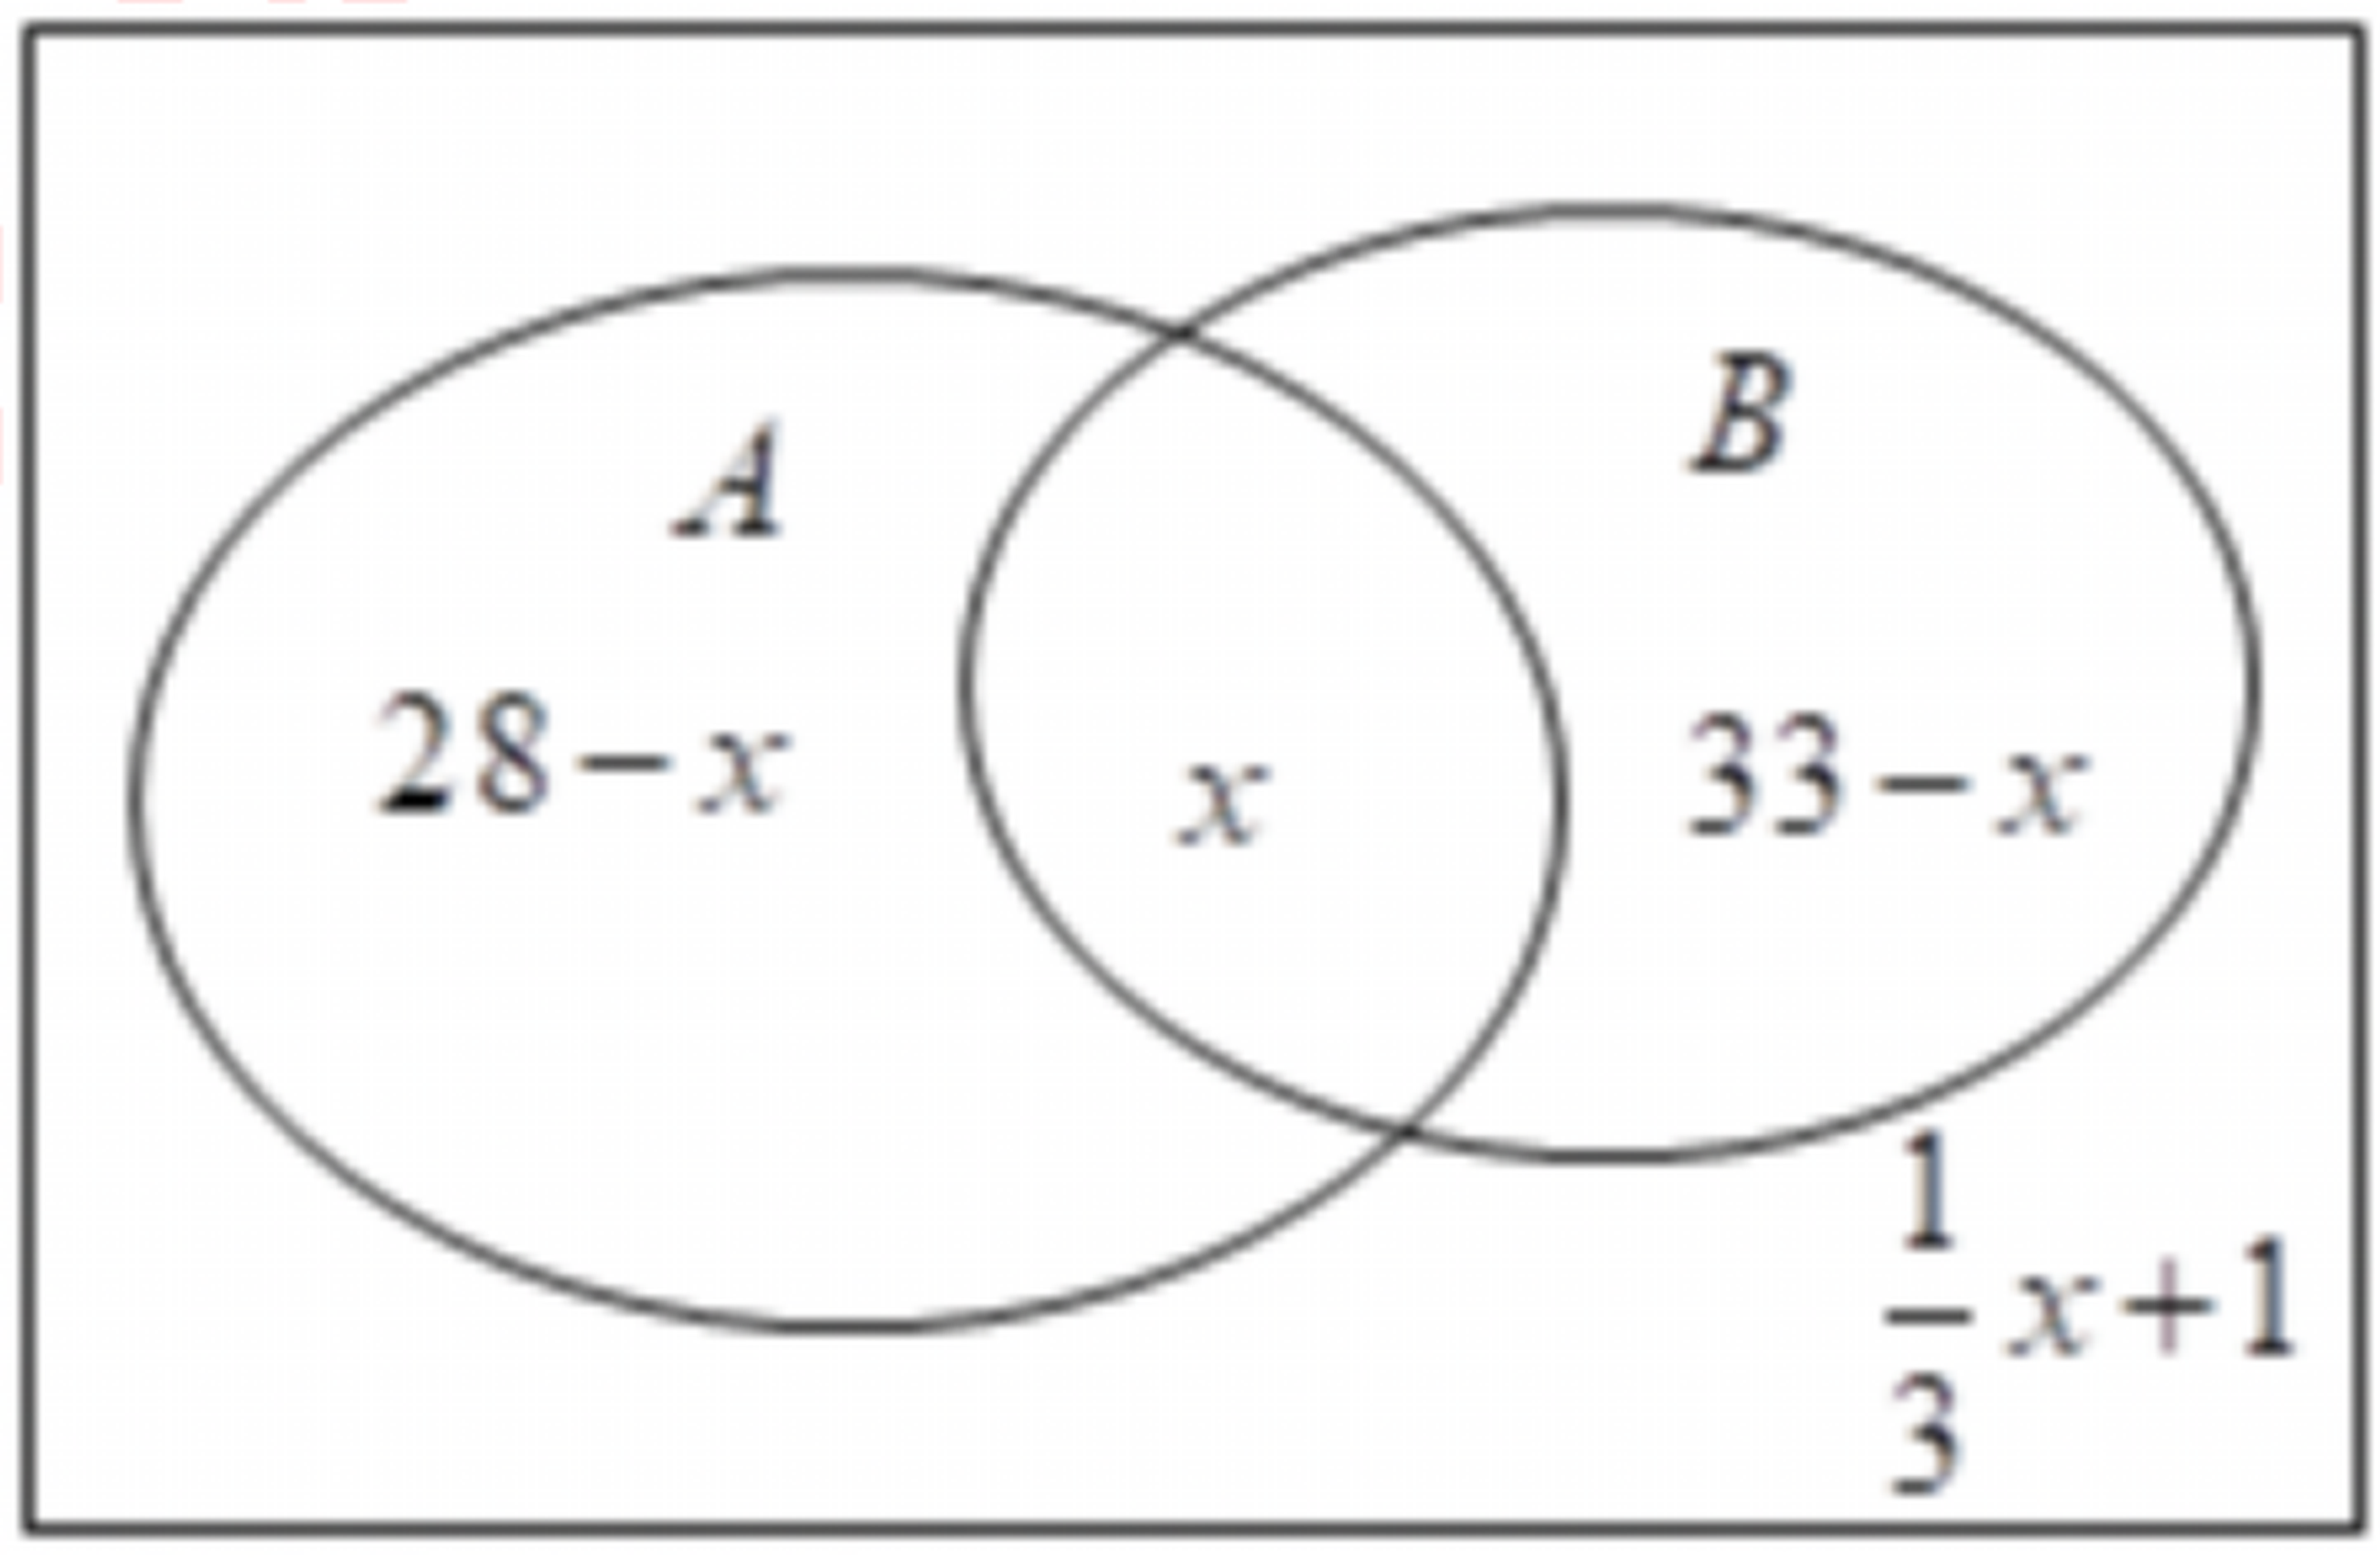
\includegraphics[width=0.42\textwidth]{figures/venn_AB_survey_50_x.png}
\end{center}
\step{则仅参加 $A$ 项的有 $(28-x)$ 人，仅参加 $B$ 项的有 $(33-x)$ 人，}
\step{$A$、$B$ 两项公益活动都不参加的有 $\left(\dfrac13x+1\right)$ 人，}
\step{由题意得 $x+(28-x)+(33-x)+\left(\dfrac13x+1\right)=50$，解得 $x=18$，}
\step{所以只参加 $A$ 项不参加 $B$ 项的有 $28-18=10$ 人.}
\solend
\fi

\item 设集合 $A=\{x\mid x^2-3x+2=0\}$，则满足 $A\cup B=\{0,1,2\}$ 的集合 $B$ 的个数是 \blankline[4.4em].

\ans{$4$}

\ifanswer
\solbegin
\step{$A=\{x\mid x^2-3x+2=0\}=\{x\mid x=1\text{ 或 }x=2\}=\{1,2\}$，}
\step{若 $A\cup B=\{0,1,2\}$，则 $0\in B$，}
\step{则 $B=\{0\},\{0,2\},\{1,0\},\{0,1,2\}$，共 $4$ 个.}
\solend
\fi

\item 已知全集 $U=\R$，集合 $A=\{x\mid x^2<4\}$，$B=\{y\mid y=x^2\}$，则图中阴影部分所表示的集合为 \blankline[4.4em].

\begin{center}
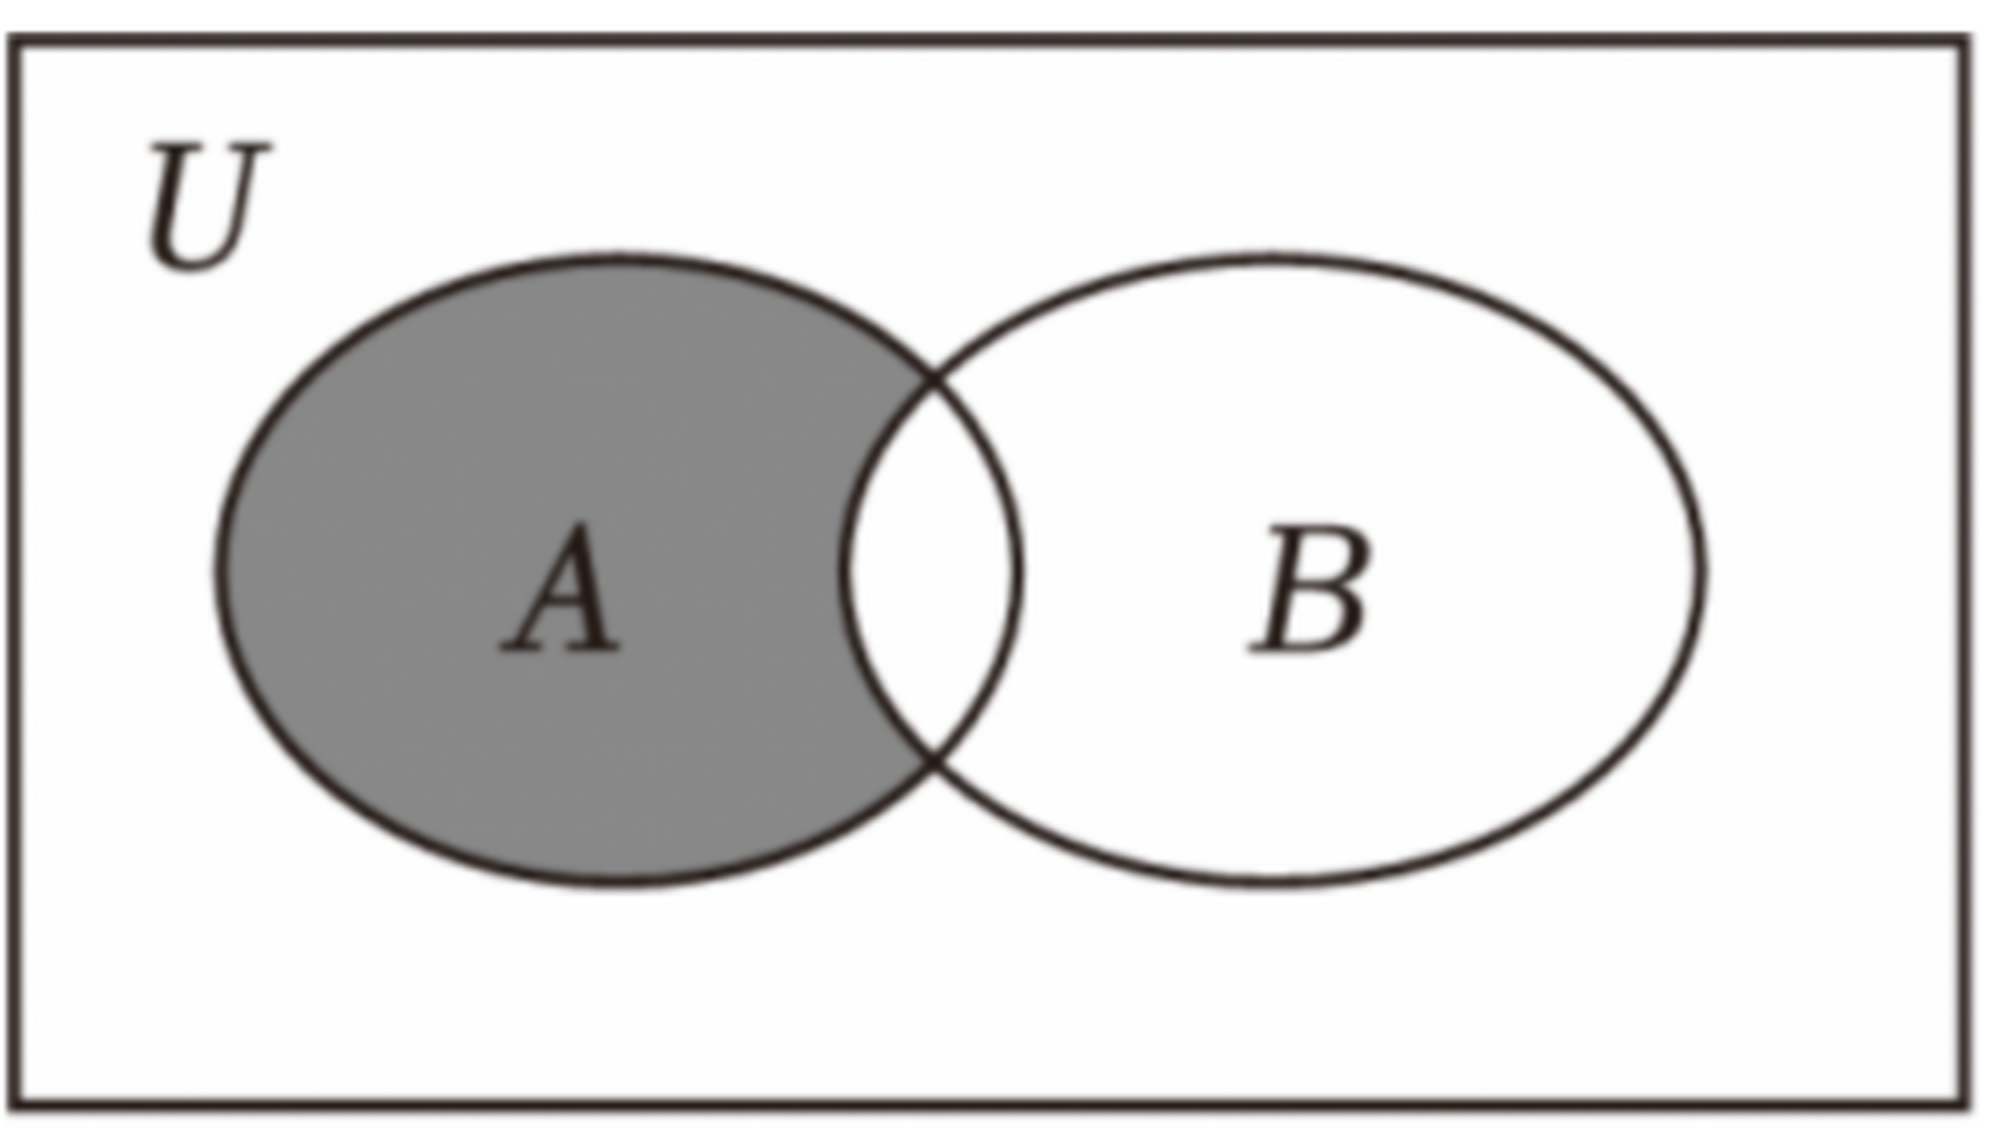
\includegraphics[width=0.34\textwidth]{figures/venn_A_shaded_U.png}
\end{center}

\ans{$A\cap\overline B=(-2,0)$}

\ifanswer
\solbegin
\step{集合 $A=\{x\mid x^2<4\}=(-2,2)$，$B=\{y\mid y=x^2\}=[0,+\infty)$，}
\step{图中阴影部分所表示的集合是 $A\cap\overline B=(-2,0)$.}
\solend
\fi

\item 如图所示，$M$、$P$、$S$ 是 $V$ 的三个子集，则阴影部分所表示的集合是 \blankline[5.4em].

\begin{center}
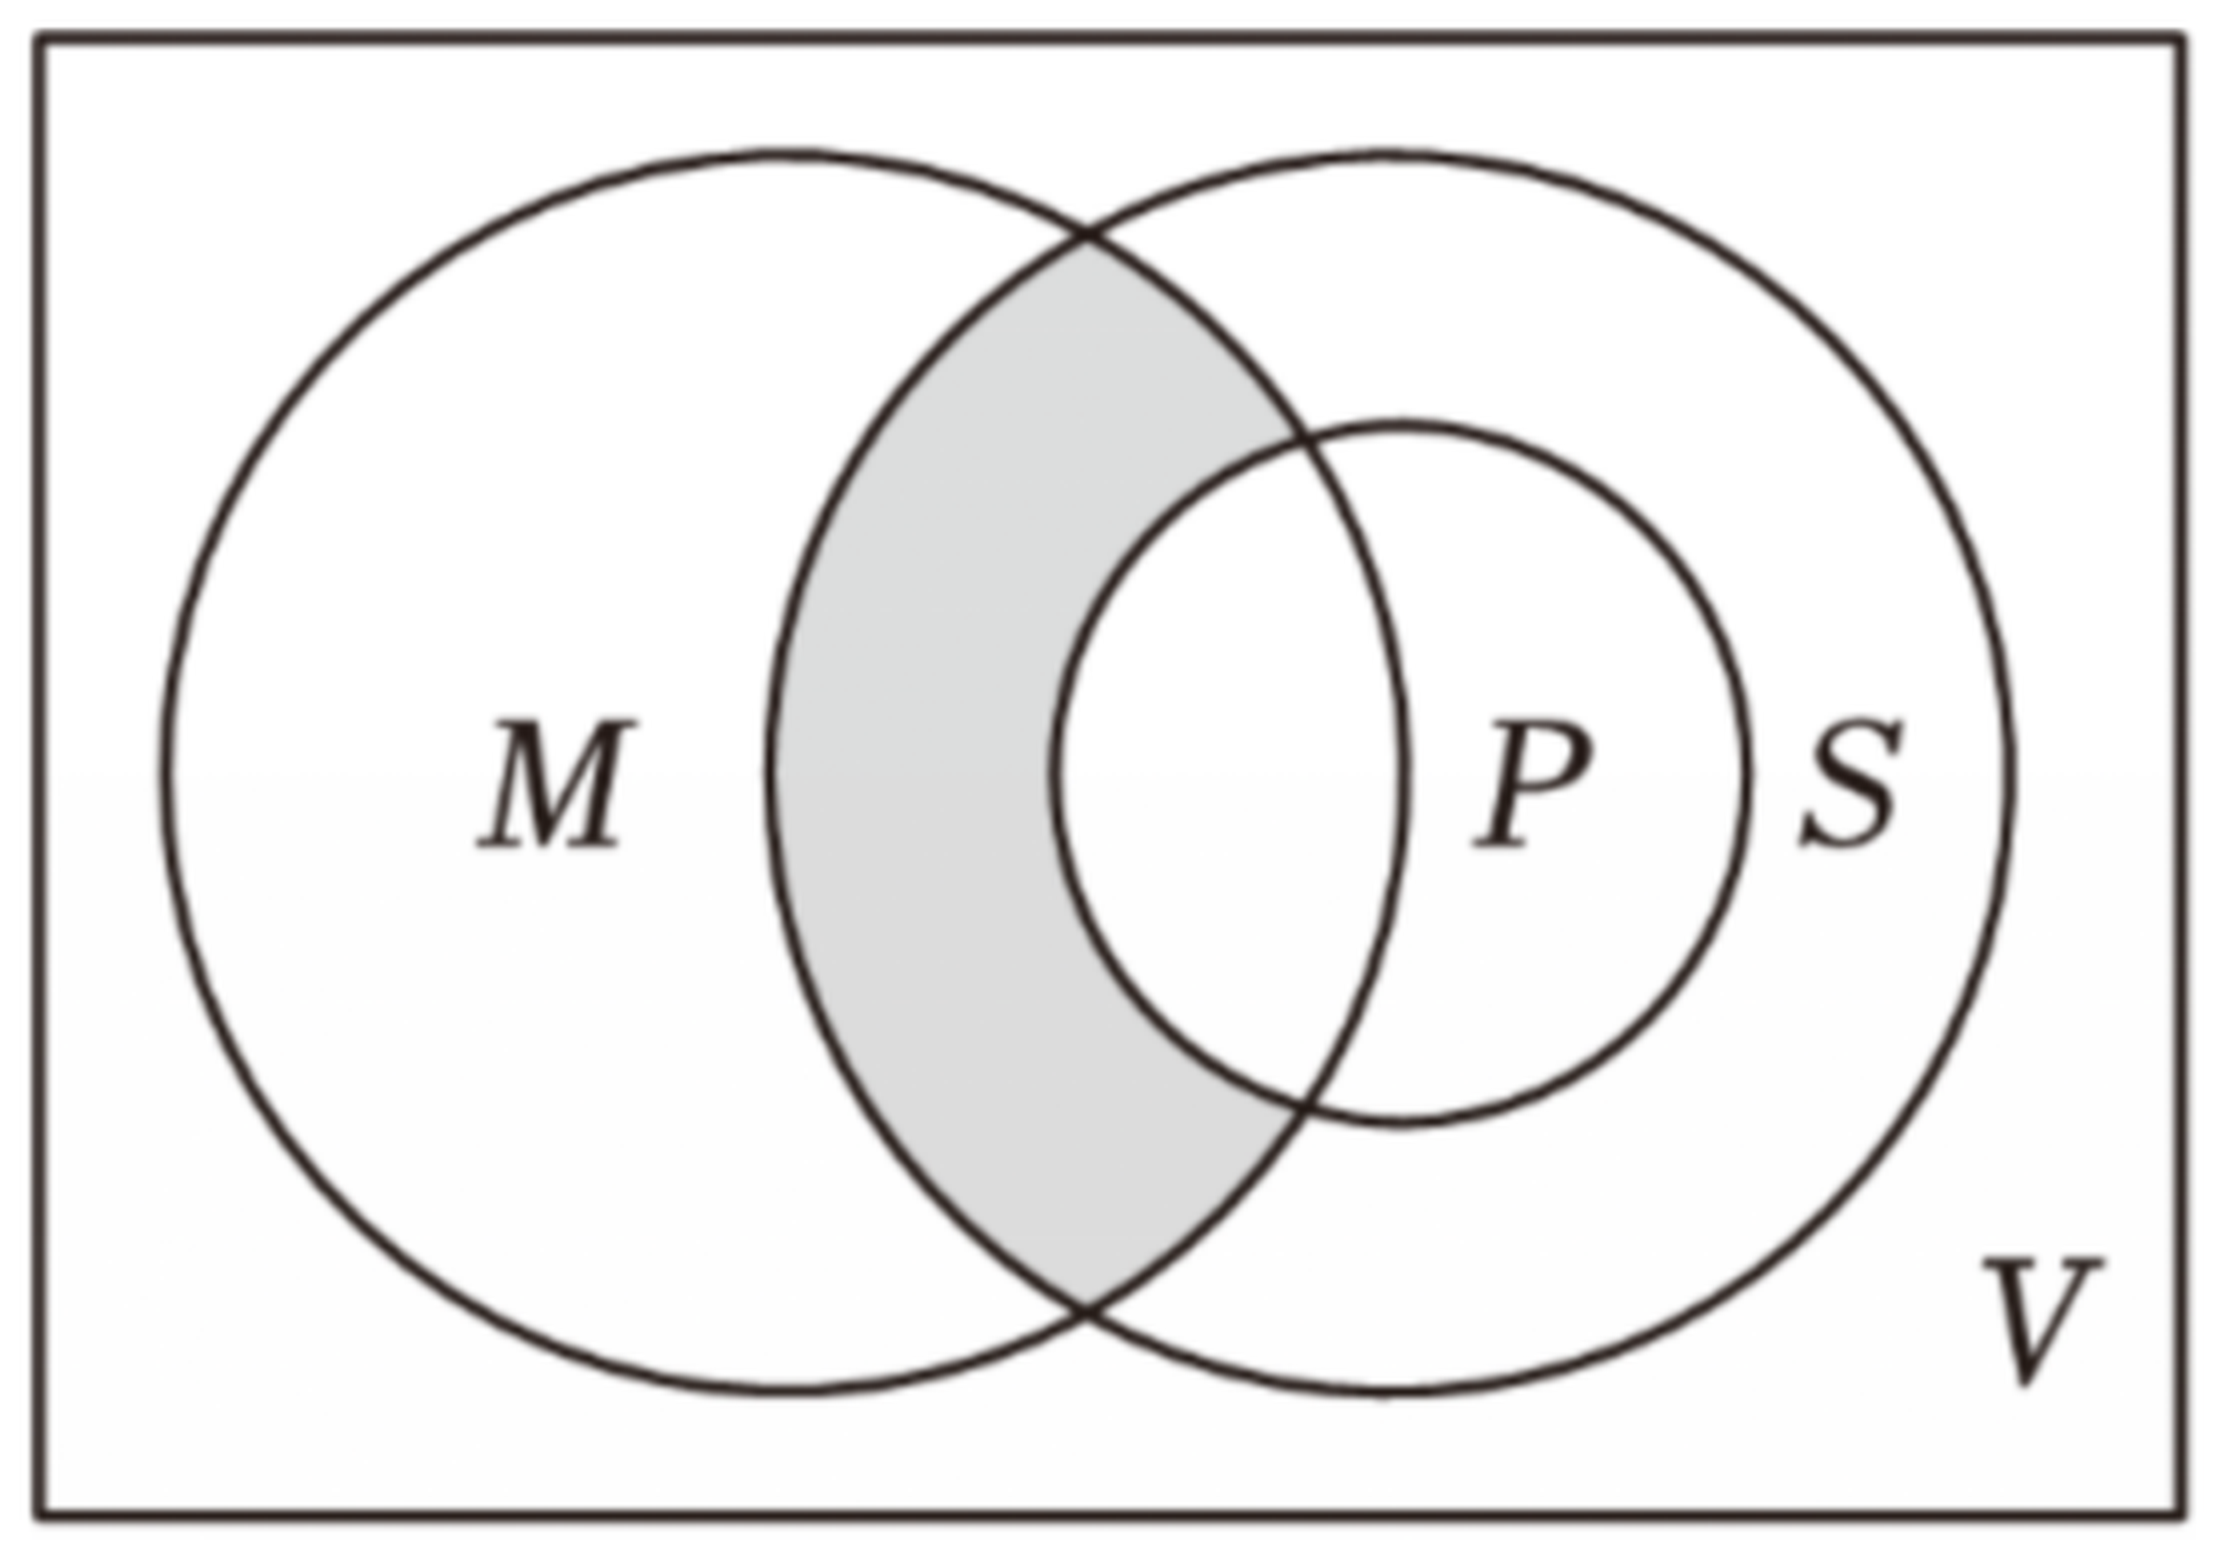
\includegraphics[width=0.38\textwidth]{figures/venn_MPS_V.png}
\end{center}

\ans{$(M\cap S)\cap(\complement_V P)$}

\item 下面六个关系式：① $\varnothing\subseteq\{a\}$；② $a\subseteq\{a\}$；③ $\{a\}\subseteq\{a\}$；④ $\{a\}\in\{a,b\}$；⑤ $a\in\{a,b,c\}$；⑥ $\varnothing\in\{a,b\}$；其中正确的是 \blankline[3.4em].

\ans{①③⑤}

\item 已知集合 $A=\{x\mid -1\le x\le a\}\ne\varnothing$，若 $\{y\mid y=x+1,x\in A\}=\{y\mid y=x^2,x\in A\}$，则实数 $a$ 值为 \blankline[4.4em].

\ans{$0$ 或 $\dfrac{1+\sqrt5}{2}$}

\ifanswer
\solbegin
\step{因为 $A=\{x\mid -1\le x\le a\}\ne\varnothing$，}
\step{所以 $\{y\mid y=x+1,x\in A\}=\{y\mid 0\le y\le a+1\}$，}
\step{$-1\le a\le1$ 时，$\{y\mid y=x^2,x\in A\}=\{y\mid 0\le y\le1\}$，}
\step{$a>1$ 时，$\{y\mid y=x^2,x\in A\}=\{y\mid 0\le y\le a^2\}$，}
\step{① $-1\le a\le1$ 时，$\{y\mid 0\le y\le a+1\}=\{y\mid 0\le y\le1\}$，则 $a+1=1$，解得 $a=0$；}
\step{② $a>1$ 时，$\{y\mid 0\le y\le a+1\}=\{y\mid 0\le y\le a^2\}$，则 $a^2=a+1$，解得 $a=\dfrac{1+\sqrt5}{2}$；}
\step{所以 $a=0$ 或 $\dfrac{1+\sqrt5}{2}$.}
\solend
\fi

\item 设集合 $A=\{(x,y)\mid x+y=22,x>0,y>0,x,y\text{ 均为质数}\}$ 的子集的个数为 \blankline[4.4em].

\ans{$32$}

\ifanswer
\solbegin
\step{集合 $A=\{(x,y)\mid x+y=22,x>0,y>0,x,y\text{ 均为质数}\}$}
\step{$=\{(3,19),(19,3),(5,17),(17,5),(11,11)\}$，则 $A$ 的子集的个数为 $2^5=32$.}
\solend
\fi

% 注：原卷本题题干印作「已知一个有四个数字元素的集合 $S$」；「数字元素」疑为「元素」之衍，
%     但原卷字形确为「数字」二字（已 3× 放大核对过），本稿照录，不代为改写。
\item 已知一个有四个数字元素的集合 $S$，$S$ 的所有子集的元素和（空集的元素和认为是 $0$）的总和为 $16192$，则 $S$ 的元素之和等于 \blankline[4.4em].

\ans{$2024$}

\ifanswer
\solbegin
\step{设 $S=\{a_1,a_2,a_3,a_4\}$，$S$ 的每个元素在所有子集中均出现 $2^3$ 次，}
\step{故 $(a_1+a_2+a_3+a_4)\cdot 2^3=16192$，所以 $a_1+a_2+a_3+a_4=2024$，}
\step{故 $S$ 的元素之和等于 $2024$.}
\solend
\fi

\item 设 $A$ 是非空数集，若对任意 $x$、$y\in A$，都有 $x+y\in A$、$xy\in A$，则称 $A$ 具有性质 $P$，给出以下命题：

①若 $A$ 具有性质 $P$，则 $A$ 可以是有限集；

②若 $A$ 具有性质 $P$，且 $A\ne\R$，则 $\overline A$ 具有性质 $P$；

③若 $A_1$、$A_2$ 具有性质 $P$，且 $A_1\cap A_2\ne\varnothing$，则 $A_1\cap A_2$ 具有性质 $P$；

④若 $A_1$、$A_2$ 具有性质 $P$，则 $A_1\cap A_2$ 具有性质 $P$.

其中所有真命题的序号是 \blankline[4.4em].

\ans{①③}

\ifanswer
\solbegin
\step{对于①，取集合 $A=\{0,1\}$ 具有性质 $P$，故 $A$ 可以是有限集，故①正确；}
\step{对于③，取 $x$、$y\in A_1\cap A_2$，则 $x\in A_1$，$x\in A_2$，$y\in A_1$，$y\in A_2$，}
\step{又 $A_1$、$A_2$ 具有性质 $P$，所以 $x+y\in A_1$，$xy\in A_1$，$x+y\in A_2$，$xy\in A_2$，}
\step{所以 $x+y\in A_1\cap A_2$，$xy\in A_1\cap A_2$，所以 $A_1\cap A_2$ 具有性质 $P$，故③正确；}
\step{对于④，取 $A_1=\{x\mid x=2k,k\in\Z\}$，$A_2=\{x\mid x=3k,k\in\Z\}$，$2\in A_1$，$3\in A_2$，}
\step{但 $2+3\notin A_1\cup A_2$，故④错误；}
\step{对于②，若 $A$ 具有性质 $P$，且 $A\ne\R$，假设 $\overline A$ 也具有性质 $P$，}
\step{设 $0\in A$，在 $\overline A$ 中任取一个 $x$，$x\ne0$，此时可证得 $-x\in A$，}
\step{否则若 $-x\in\overline A$，由于 $\overline A$ 也具有性质 $P$，则 $x+(-x)=0\in\overline A$，}
\step{与 $0\in A$ 矛盾，故 $-x\in A$，}
\step{由于 $A$ 具有性质 $P$，$\overline A$ 也具有性质 $P$，所以 $(-x)^2\in A$，$x^2\in\overline A$，}
\step{而 $(-x)^2=x^2$，这与 $A\cap\overline A=\varnothing$ 矛盾，}
\step{故当 $0\in A$ 且 $A$ 具有性质 $P$ 时，则 $\overline A$ 不具有性质 $P$，}
\step{同理当 $0\in\overline A$ 时，也可以类似推出矛盾，故②错误.}
\step{故正确的是①③.}
\solend
\fi

\item 已知 $S=\{1,2,3,4,5\}$，$A=\{1,2,5\}$，$T=\{t_1,t_2\}\subseteq S$，记 $A_1=\{x\mid x=a+t_1,a\in A,t_1\in T\}$，$A_2=\{x\mid x=b+t_2,b\in A,t_2\in T\}$，若 $A_1\cap A_2=\varnothing$，则集合 $T$ 为 \blankline[5.4em].

\ans{$T=\{1,3\}$ 或 $T=\{2,4\}$ 或 $T=\{3,5\}$}

\ifanswer
\solbegin
\step{若 $A_1\cap A_2=\varnothing$，即 $a+t_1\ne b+t_2$，则 $t_1-t_2\ne a-b$，其中 $a$、$b\in A$，}
\step{否则 $t_1+a=t_2+b$，$A_1\cap A_2\ne\varnothing$，}
\step{又 $S=\{1,2,3,4,5\}$，$A=\{1,2,5\}$，$T=\{t_1,t_2\}\subseteq S$，}
\step{$2-1=1$，$5-2=3$，$5-1=4$，则 $t_1$、$t_2$ 相差 $2$，}
\step{所以 $T=\{1,3\}$ 或 $T=\{2,4\}$ 或 $T=\{3,5\}$.}
\solend
\fi

\end{enumerate}

\bigsec{二、解答题}

\begin{enumerate}
\setcounter{enumi}{13}

\item 设集合 $P=\{1,2,3,m\}$，$Q=\{3,m^2\}$，且 $\overline P\cap Q=\varnothing$，求实数 $m$ 的值组成的集合.

\ans{$\{-1,0,\pm\sqrt2\}$}

\ansspace[5]

\ifanswer
\solbegin
\step{因为 $\overline P\cap Q=\varnothing$，所以 $Q\subseteq P$，所以 $m^2=1$ 或 $m^2=2$ 或 $m^2=m$，}
\step{考虑互异性，得 $m=-1$ 或 $m=\pm\sqrt2$ 或 $m=0$，}
\step{所以实数 $m$ 的值组成的集合为 $\{-1,0,\pm\sqrt2\}$.}
\solend
\fi

\item 若集合 $A=(-\infty,2]$，$B=\{x\mid kx+1<0,k\in\R\}$，$A\cap B=\varnothing$，求实数 $k$ 的取值范围.

\ans{$\left[-\dfrac12,0\right]$}

\ansspace[5]

\ifanswer
\solbegin
\step{若 $B=\varnothing$，则 $k=0$，符合题意，}
\step{若 $B\ne\varnothing$，当 $k>0$ 时，$B=\left(-\infty,-\dfrac1k\right)$，$A\cap B\ne\varnothing$，不合题意；}
\step{当 $k<0$ 时，$B=\left(-\dfrac1k,+\infty\right)$，由 $A\cap B=\varnothing$ 得 $-\dfrac1k\ge2$，即 $-\dfrac12\le k<0$，}
\step{故 $k$ 的取值范围是 $\left[-\dfrac12,0\right]$.}
\solend
\fi

\item 已知集合 $A=\{-4,2a-1,a^2\}$，$B=\{a-5,1-a,9\}$，分别求适合下列条件的 $a$ 的值.

% 两个小问不许与题干分家：试卷版第 2 页页末原本正好把 (1) 留在页底、(2) 翻到次页，
% 与 2026-09-15 修的三类难看切页同源，故在这里也加 \keepwithprev 守卫（三版都生效）。
\keepwithprev
（1）$9\in(A\cap B)$；

\keepwithprev
（2）$\{9\}=A\cap B$.

\ans{（1）$a=5$ 或 $a=-3$；（2）$a=-3$}

\ansspace[5]

\ifanswer
\solbegin
\stepm{（1）}{$9\in(A\cap B)$，所以 $9\in A$，}
\step{当 $2a-1=9$ 时，$a=5$，当 $a^2=9$ 时，即 $a=\pm3$，}
% 注：原卷此句结论印作「所以 $a$ 的值为 $5\backslash-3$」——「\」应是顿号之误，
%     本稿照录原卷字形（见文件头「原卷存疑」②）；按文意即 $a=5$ 或 $a=-3$。
\step{当 $a=3$ 时，$a-5=1-a$ 舍去，所以 $a$ 的值为 $5\backslash-3$.}
\stepm{（2）}{结合（1）的结论：}
\step{当 $2a-1=9$ 即 $a=5$ 时，$1-a=-4$，$\{9\}\ne(A\cap B)$，}
\step{当 $a^2=9$ 时，即 $a=\pm3$，当 $a=3$ 时，$a-5=1-a$ 舍去，}
\step{所以 $a$ 的值为 $-3$.}
\solend
\fi

\item 已知集合 $M=\{a,ab,a-b\}$，$N=\{0,|a|,b\}$，且 $M=N$，求实数 $a$、$b$ 的值.

\ans{$a=b=-1$}

\ansspace[5]

\ifanswer
\solbegin
\step{由集合元素的互异性，得 $a\ne0$，且 $b\ne0$，所以 $a-b=0$，即 $a=b$，}
\step{所以 $ab=|a|$，又由 $|a|\ne b=a$，得 $a<0$，故 $a=b=-1$.}
\solend
\fi

\item 已知集合 $A=\{x\mid -2<x<7\}$，$B=\{x\mid m+1\le x\le 2m-1\}$.

\keepwithprev
（1）当 $m=4$ 时，求 $A\cap B$、$A\cup B$；

\keepwithprev
（2）若 $A\cap B=B$，求实数 $m$ 的取值范围.

\ans{（1）$A\cap B=[5,7)$，$A\cup B=(-2,7]$；（2）$(-\infty,4)$}

\ansspace[5]

\ifanswer
\solbegin
\stepm{（1）}{当 $m=4$ 时，得集合 $A=\{x\mid -2<x<7\}$，$B=\{x\mid 5\le x\le7\}$，}
\step{得 $A\cap B=[5,7)$，$A\cup B=(-2,7]$.}
\stepm{（2）}{由 $A\cap B=B$ 得 $B\subseteq A$，}
\step{①当 $B=\varnothing$ 时，得 $m+1>2m-1$，解得 $m<2$；}
\step{②当 $B\ne\varnothing$ 时，得 $\begin{cases}m+1>-2\\ 2m-1<7\\ m+1\le2m-1\end{cases}$，解得 $2\le m<4$；}
\step{综上，实数 $m$ 的取值范围是 $(-\infty,4)$.}
\solend
\fi

\item 若集合 $A=\{x\mid x^2+5x-6=0\}$，$B=\{x\mid x^2+2(m+1)x+m^2-3=0\}$.

\keepwithprev
（1）当 $m=0$ 时，求集合 $A\cup B$；

\keepwithprev
（2）若 $A\cap B=B$，求实数 $m$ 的取值范围.

\ans{（1）$A\cup B=\{1,-6,-3\}$；（2）$\{m\mid m\le-2\}$}

\ansspace[5]

\ifanswer
\solbegin
\stepm{（1）}{由题意得，集合 $A=\{x\mid x^2+5x-6=0\}=\{1,-6\}$，}
\step{当 $m=0$ 时，$B=\{x\mid x^2+2x-3=0\}=\{1,-3\}$，}
\step{所以 $A\cup B=\{1,-6,-3\}$；}
\stepm{（2）}{由（1）得集合 $A=\{1,-6\}$，$B=\{x\mid x^2+2(m+1)x+m^2-3=0\}$，}
\step{若 $A\cap B=B$ 得 $B\subseteq A$，所以 $B=\varnothing$ 或 $\{-6\}$ 或 $\{1\}$ 或 $\{1,-6\}$，}
\step{当 $B=\varnothing$ 时，$\Delta=4(m+1)^2-4(m^2-3)<0$，解得 $m<-2$，}
\step{当 $B=\{-6\}$ 时，则 $\begin{cases}\Delta=4(m+1)^2-4(m^2-3)=0\\ 36-12(m+1)+m^2-3=0\end{cases}$，无解，}
\step{当 $B=\{1\}$ 时，则 $\begin{cases}\Delta=4(m+1)^2-4(m^2-3)=0\\ 1+2(m+1)+m^2-3=0\end{cases}$，解得 $m=-2$，}
\step{当 $B=\{1,-6\}$ 时，则 $\begin{cases}\Delta=4(m+1)^2-4(m^2-3)>0\\ 1+(-6)=-2(m+1)\\ 1\times(-6)=m^2-3\end{cases}$，无解，}
\step{综上所述，实数 $m$ 的取值范围为 $\{m\mid m\le-2\}$.}
\solend
\fi

% 压轴题：其后已无内容，故作答区全用可丢弃胶水（\ansspace*），并在题目前先量一下版面。
\ansneed{8cm}
\item 对于点集 $A=\{(x,y)\mid x=m,y=-3x+2,m\in\N,m\ge1\}$，$B=\{(x,y)\mid x=n,y=a(x^2-x+1),n\in\N,n\ge1\}$，是否存在非零整数 $a$，使得 $A\cap B\ne\varnothing$？

\ans{$a=-1$}

\ansspace*[10]

\ifanswer
\solbegin
\step{当 $A\cap B\ne\varnothing$ 时，$-3x+2=a(x^2-x+1)$，}
\step{$ax^2+(3-a)x+a-2=0$ ①有正整数解，}
\step{所以 $\Delta=(3-a)^2-4a(a-2)=-3a^2+2a+9$ 是平方数，}
\step{所以 $3a^2-2a-9\le0$，$\dfrac{1-2\sqrt7}{3}\le a\le\dfrac{1+2\sqrt7}{3}$，$a\ne0$，$a\in\Z$，}
\step{所以 $a=\pm1$ 或 $a=2$，}
\step{$a=-1$ 时 $\Delta=4$，这时①变为 $-x^2+4x-3=0$，解得 $x_1=1$，$x_2=3$，}
\step{$A\cap B=\{(1,-1),(3,-7)\}$.}
\step{$a=1$ 时 $\Delta=8$，不是平方数.}
\step{$a=2$ 时 $\Delta=1$，这时①变为 $2x^2+x=0$，没有正整数解.}
\step{所以 $a=-1$.}
\solend
\fi

\end{enumerate}

\end{document}
"
% 紧凑版：xelatex "\def\iscompact{1}% 高一19_延安中学_周末作业2.tex —— 高一上数学「2026-2027 年延安中学高一上周末作业 2」（试卷版/答案版）
% 试卷版：xelatex 高一19_延安中学_周末作业2.tex
% 答案版：xelatex "\def\isanswer{1}% 高一19_延安中学_周末作业2.tex —— 高一上数学「2026-2027 年延安中学高一上周末作业 2」（试卷版/答案版）
% 试卷版：xelatex 高一19_延安中学_周末作业2.tex
% 答案版：xelatex "\def\isanswer{1}\input{高一19_延安中学_周末作业2.tex}"
% 紧凑版：xelatex "\def\iscompact{1}\input{高一19_延安中学_周末作业2.tex}"
%
% 原始材料是微信公众号图文（公众号「魔都数学加油站」，作者署名「破晓」，
% 原文链接 https://mp.weixin.qq.com/s/tHqWSV1StO5SHSXXQ4jeUA），正文为 6 张 PNG 页；
% 原文本身就是一份**讲评版**——题目下方直接印出【答案】或【解析】。本稿把答案与解析
% 移到答案版，试卷版即一张干净的空卷；试题文字、答案与解析均照原卷录入。
%
% 与原卷的排版差异（均已在 README「说明」中交代）：
%   ① 原文自**第 3 题**起（第 1、2 题未在该文发布），源码里以 \setcounter{enumi}{2} 起编；
%      全卷只有「一、填空题」「二、解答题」两节，无选择题；
%   ② 原卷本就印有两个分节标题（已在原图上逐页放大核对过），本稿照原卷分节，只把标题改排
%      成全稿统一的「大节标题」样式；
%   ③ 原卷的实数集、整数集、自然数集符号作正体 $R$、$Z$、$N$（第 15 题作粗体 $\mathbf{R}$，
%      第 20 题有 $N$ 与斜体 $Z$），本稿按全稿惯例统一写作 $\R$、$\Z$、$\N$；
%   ④ 第 4 题的韦恩图在原卷里印在【解析】右侧（题干并无「如图」二字），故本稿把该图放进
%      答案版的解析块内（`figures/venn_AB_survey_50_x.png`）；第 6、7 题的韦恩图是**题干图**
%      （题干作「图中阴影部分所表示的集合」），两版都排（`figures/venn_A_shaded_U.png`、
%      `figures/venn_MPS_V.png`）。三张图都取自原卷截图、4× LANCZOS 放大，不用 TikZ 手绘；
%   ⑤ 本卷也是「讲评版」，解析按全稿统一的 \solbegin/\step 分步重排（原卷为连续段落），
%      分步不改一字，只断句、断行；
%   ⑥ 标题前缀照**原卷**作「2026--2027 年…」（原卷标题即作「2026-2027年延安中学高一上周末
%      作业 2」）。同校的 高一06 作「学年度」——那是 高一02—高一09 那一批入库时统一改的；
%      后续入库的卷（高一10—高一17 与本卷）一律照原卷保留「年」，未强改，故同校两卷前缀不同。
%
% 原卷存疑两处（已逐处放大到能看清字形后核对，本稿照录并加注，见各题下的 `%` 注）：
%   （另有第三处「第 12 题【解析】末句」原先记作存疑，2026-09-26 第二轮核对放大后发现
%     原卷印的是「$0\in\overline A$」——A 上确有横杠，是本稿当初漏抄了 $\overline{}$；
%     已按原卷补回，故该条从存疑清单里删去，不计为原卷问题。）
%   ① 第 11 题题干印作「已知一个有四个数字元素的集合 $S$」，「数字元素」疑为「元素」之衍；
%   ② 第 16 题 (1) 结论印作「$a$ 的值为 $5\backslash-3$」，其中的「\」应是顿号之误
%      （由 (2) 的结论「$a$ 的值为 $-3$」可反推，(1) 的答案是 $5$ 或 $-3$）；

% 本篇在公众号「魔都数学加油站」连载里的编号是「27学年高一19」，本地编号与之对齐（高一19）；
% 对应关系见 README「与公众号连载号的对照表」。
\documentclass[a4paper,11pt]{article}
\usepackage{common}

\begin{document}

\examtitlest{2026--2027 年延安中学高一上周末作业 2}{集合与常用逻辑用语}

\bigsec{一、填空题}

\begin{enumerate}
% 原卷填空题从第 3 题起（1、2 未在该文中发布），须与解答题的 \setcounter{enumi}{13} 对齐
\setcounter{enumi}{2}
\item 已知全集 $U=\{1,2,3,4,5\}$，$M=\{1,2\}$，$P=\{1,3,5\}$，则 $M\cap\overline P=$ \blankline[4.4em].

\ans{$\{2\}$}

\item 某公司共有 $50$ 人，此次组织参加社会公益活动，其中参加 $A$ 项公益活动的有 $28$ 人，参加 $B$ 项公益活动的有 $33$ 人，且 $A$、$B$ 两项公益活动都不参加的人数比都参加的人数的三分之一多 $1$ 人，则只参加 $A$ 项不参加 $B$ 项的人数是 \blankline[4.4em].

\ans{$10$}

\ifanswer
\solbegin
\step{如图所示，设 $A$、$B$ 两项公益活动都参加的有 $x$ 人，}
\begin{center}
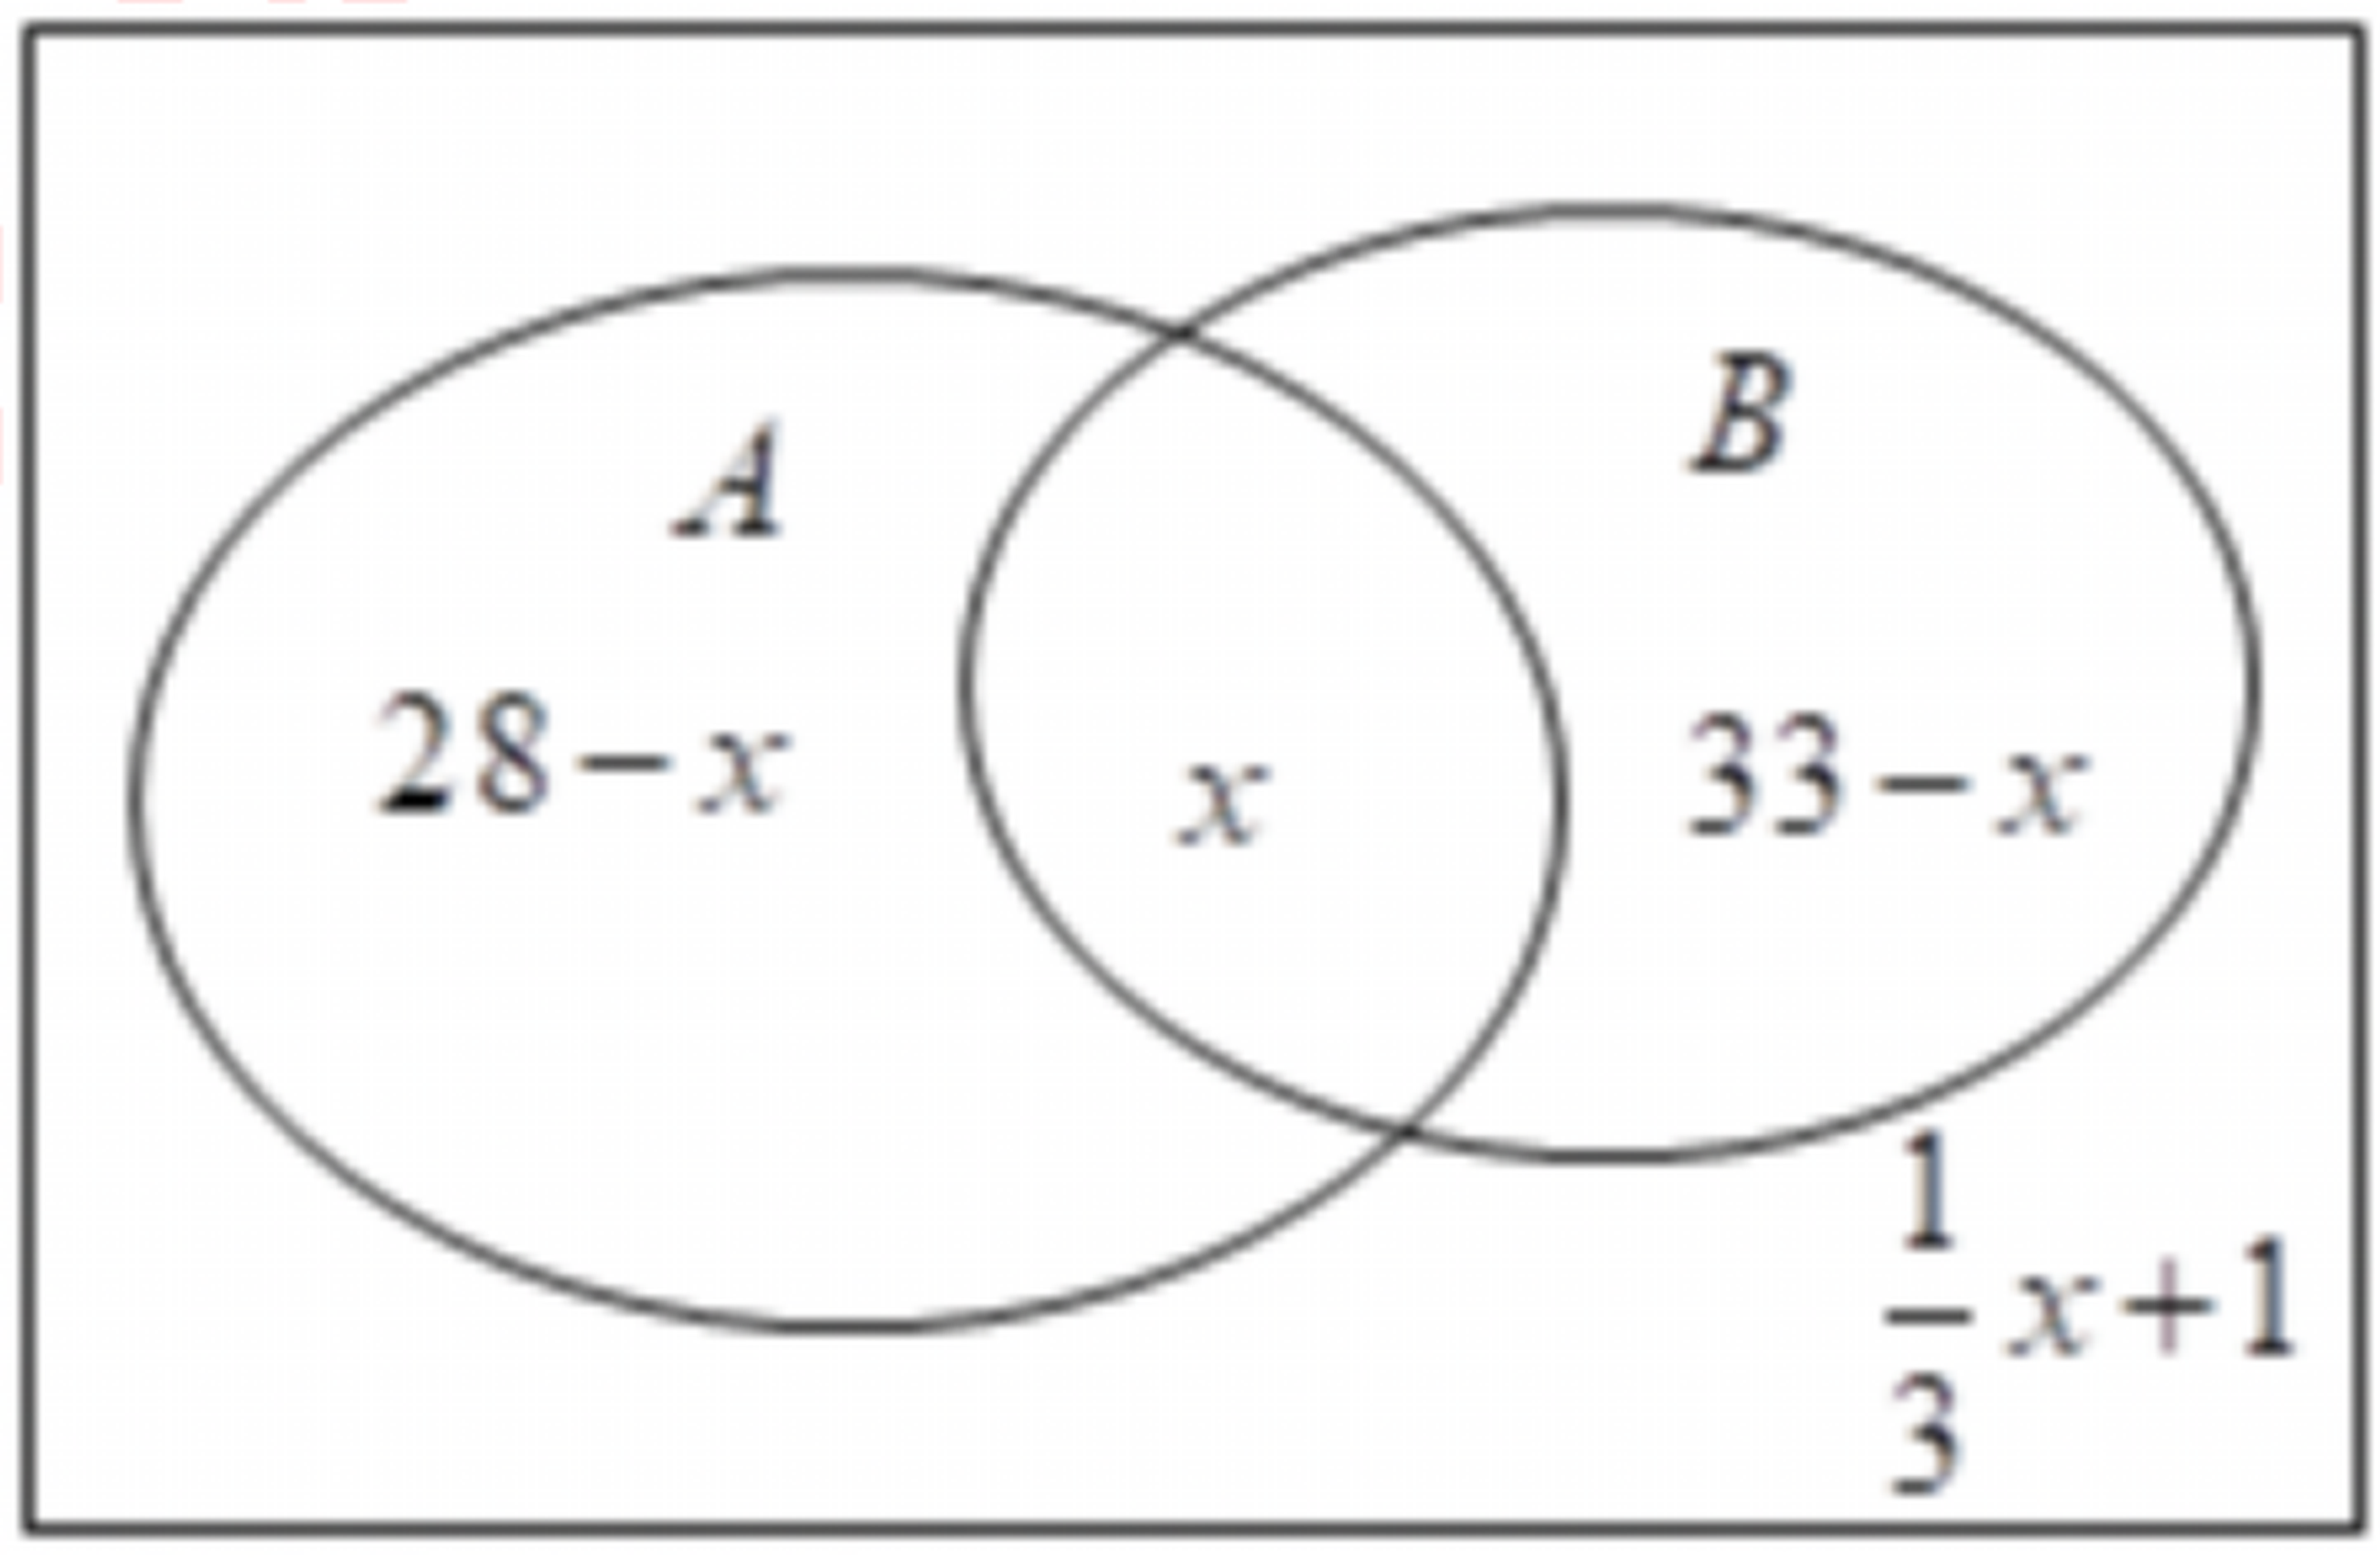
\includegraphics[width=0.42\textwidth]{figures/venn_AB_survey_50_x.png}
\end{center}
\step{则仅参加 $A$ 项的有 $(28-x)$ 人，仅参加 $B$ 项的有 $(33-x)$ 人，}
\step{$A$、$B$ 两项公益活动都不参加的有 $\left(\dfrac13x+1\right)$ 人，}
\step{由题意得 $x+(28-x)+(33-x)+\left(\dfrac13x+1\right)=50$，解得 $x=18$，}
\step{所以只参加 $A$ 项不参加 $B$ 项的有 $28-18=10$ 人.}
\solend
\fi

\item 设集合 $A=\{x\mid x^2-3x+2=0\}$，则满足 $A\cup B=\{0,1,2\}$ 的集合 $B$ 的个数是 \blankline[4.4em].

\ans{$4$}

\ifanswer
\solbegin
\step{$A=\{x\mid x^2-3x+2=0\}=\{x\mid x=1\text{ 或 }x=2\}=\{1,2\}$，}
\step{若 $A\cup B=\{0,1,2\}$，则 $0\in B$，}
\step{则 $B=\{0\},\{0,2\},\{1,0\},\{0,1,2\}$，共 $4$ 个.}
\solend
\fi

\item 已知全集 $U=\R$，集合 $A=\{x\mid x^2<4\}$，$B=\{y\mid y=x^2\}$，则图中阴影部分所表示的集合为 \blankline[4.4em].

\begin{center}
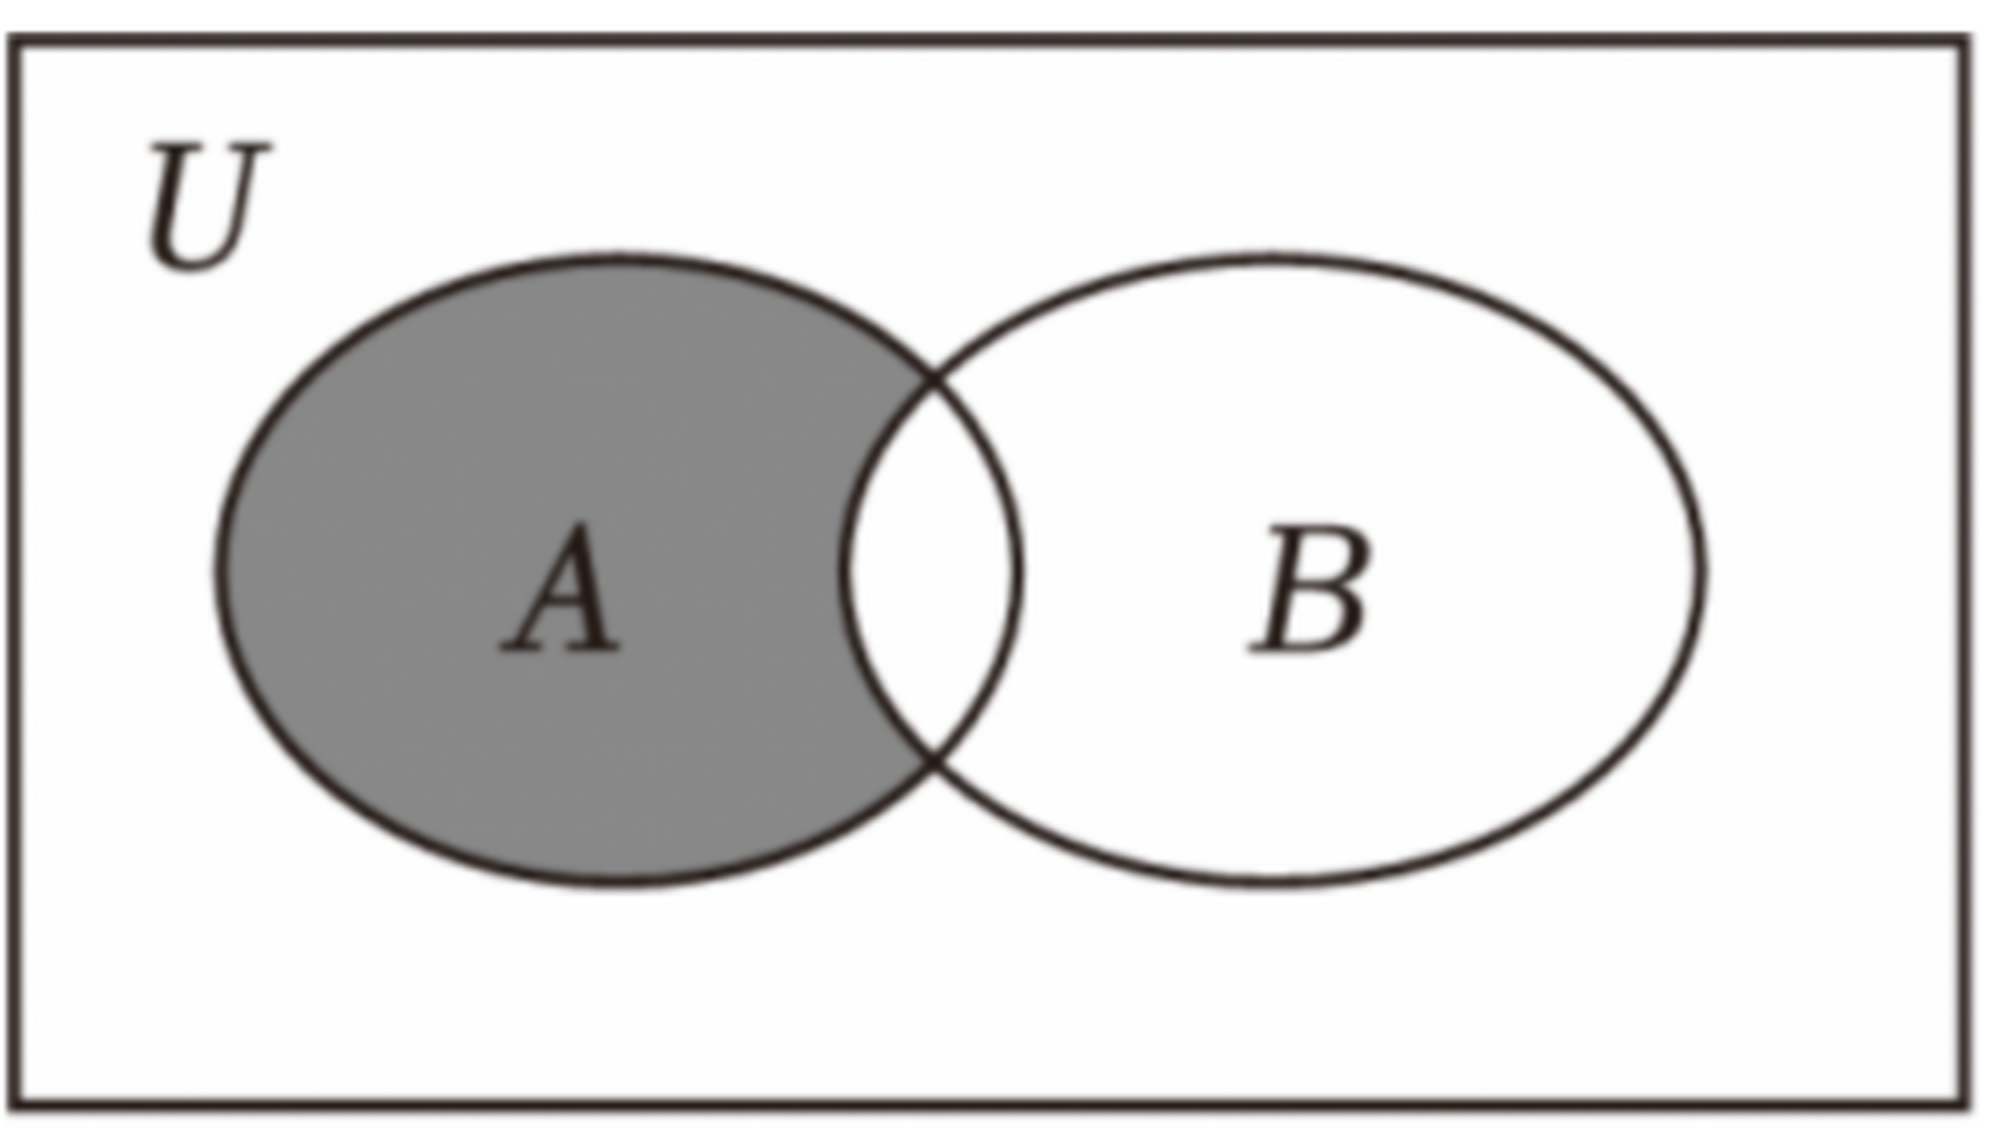
\includegraphics[width=0.34\textwidth]{figures/venn_A_shaded_U.png}
\end{center}

\ans{$A\cap\overline B=(-2,0)$}

\ifanswer
\solbegin
\step{集合 $A=\{x\mid x^2<4\}=(-2,2)$，$B=\{y\mid y=x^2\}=[0,+\infty)$，}
\step{图中阴影部分所表示的集合是 $A\cap\overline B=(-2,0)$.}
\solend
\fi

\item 如图所示，$M$、$P$、$S$ 是 $V$ 的三个子集，则阴影部分所表示的集合是 \blankline[5.4em].

\begin{center}
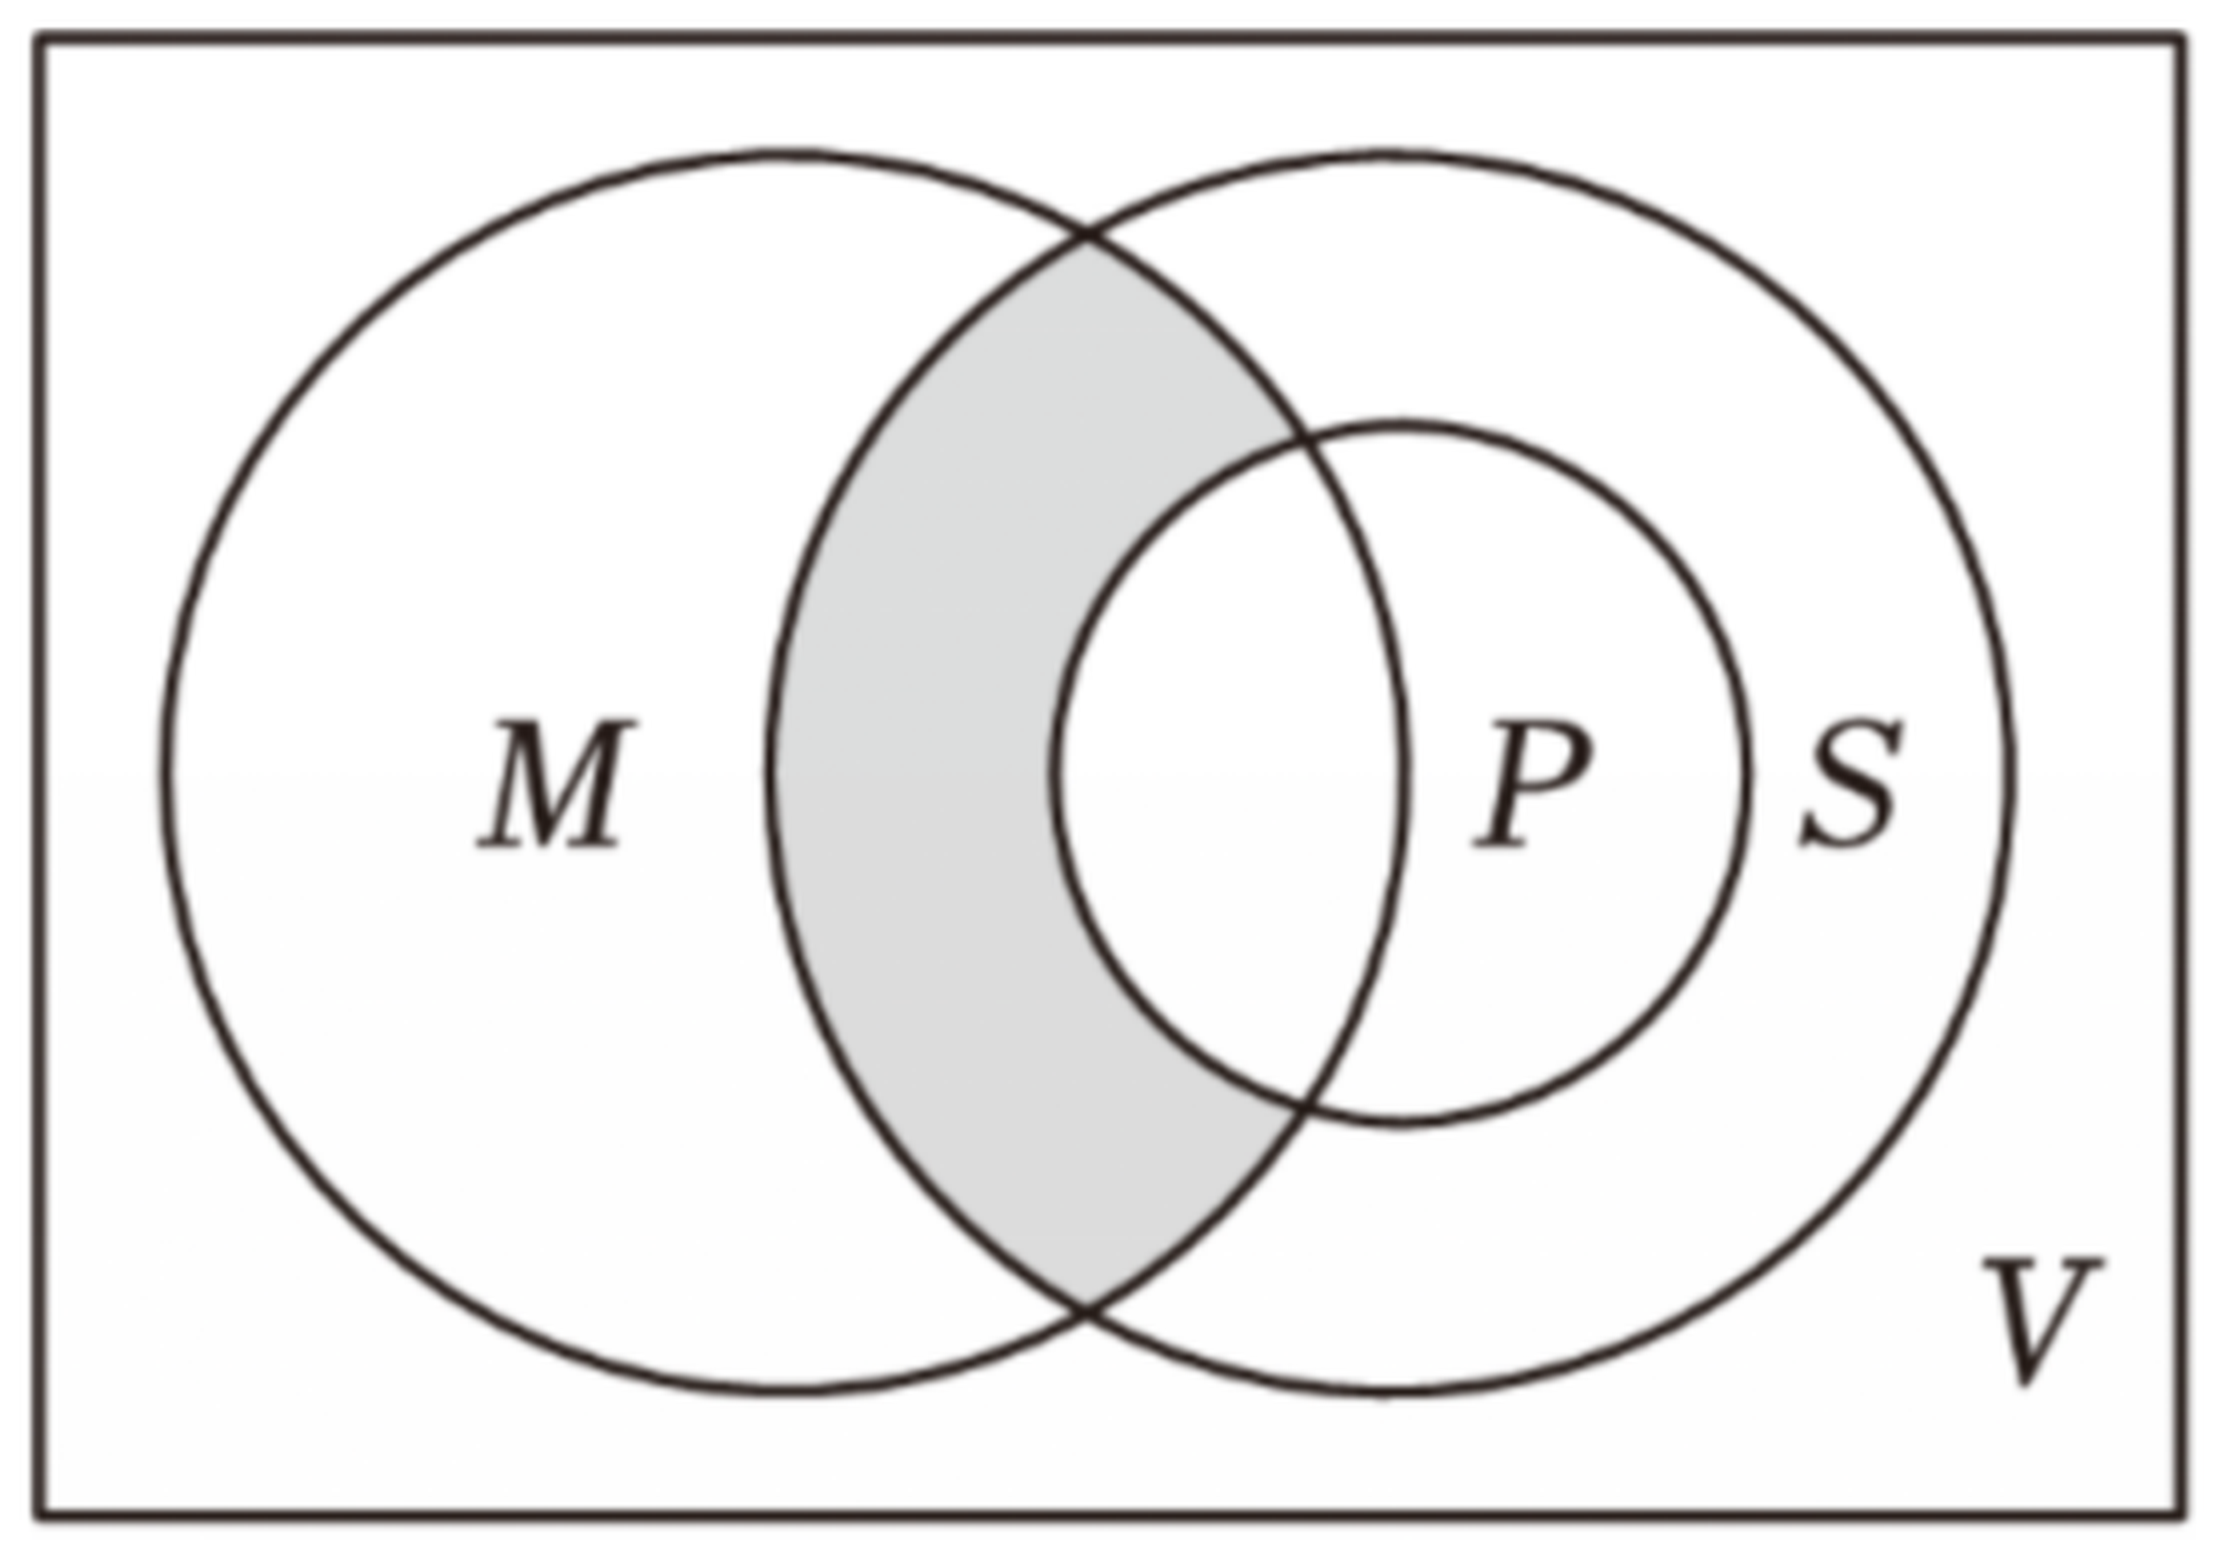
\includegraphics[width=0.38\textwidth]{figures/venn_MPS_V.png}
\end{center}

\ans{$(M\cap S)\cap(\complement_V P)$}

\item 下面六个关系式：① $\varnothing\subseteq\{a\}$；② $a\subseteq\{a\}$；③ $\{a\}\subseteq\{a\}$；④ $\{a\}\in\{a,b\}$；⑤ $a\in\{a,b,c\}$；⑥ $\varnothing\in\{a,b\}$；其中正确的是 \blankline[3.4em].

\ans{①③⑤}

\item 已知集合 $A=\{x\mid -1\le x\le a\}\ne\varnothing$，若 $\{y\mid y=x+1,x\in A\}=\{y\mid y=x^2,x\in A\}$，则实数 $a$ 值为 \blankline[4.4em].

\ans{$0$ 或 $\dfrac{1+\sqrt5}{2}$}

\ifanswer
\solbegin
\step{因为 $A=\{x\mid -1\le x\le a\}\ne\varnothing$，}
\step{所以 $\{y\mid y=x+1,x\in A\}=\{y\mid 0\le y\le a+1\}$，}
\step{$-1\le a\le1$ 时，$\{y\mid y=x^2,x\in A\}=\{y\mid 0\le y\le1\}$，}
\step{$a>1$ 时，$\{y\mid y=x^2,x\in A\}=\{y\mid 0\le y\le a^2\}$，}
\step{① $-1\le a\le1$ 时，$\{y\mid 0\le y\le a+1\}=\{y\mid 0\le y\le1\}$，则 $a+1=1$，解得 $a=0$；}
\step{② $a>1$ 时，$\{y\mid 0\le y\le a+1\}=\{y\mid 0\le y\le a^2\}$，则 $a^2=a+1$，解得 $a=\dfrac{1+\sqrt5}{2}$；}
\step{所以 $a=0$ 或 $\dfrac{1+\sqrt5}{2}$.}
\solend
\fi

\item 设集合 $A=\{(x,y)\mid x+y=22,x>0,y>0,x,y\text{ 均为质数}\}$ 的子集的个数为 \blankline[4.4em].

\ans{$32$}

\ifanswer
\solbegin
\step{集合 $A=\{(x,y)\mid x+y=22,x>0,y>0,x,y\text{ 均为质数}\}$}
\step{$=\{(3,19),(19,3),(5,17),(17,5),(11,11)\}$，则 $A$ 的子集的个数为 $2^5=32$.}
\solend
\fi

% 注：原卷本题题干印作「已知一个有四个数字元素的集合 $S$」；「数字元素」疑为「元素」之衍，
%     但原卷字形确为「数字」二字（已 3× 放大核对过），本稿照录，不代为改写。
\item 已知一个有四个数字元素的集合 $S$，$S$ 的所有子集的元素和（空集的元素和认为是 $0$）的总和为 $16192$，则 $S$ 的元素之和等于 \blankline[4.4em].

\ans{$2024$}

\ifanswer
\solbegin
\step{设 $S=\{a_1,a_2,a_3,a_4\}$，$S$ 的每个元素在所有子集中均出现 $2^3$ 次，}
\step{故 $(a_1+a_2+a_3+a_4)\cdot 2^3=16192$，所以 $a_1+a_2+a_3+a_4=2024$，}
\step{故 $S$ 的元素之和等于 $2024$.}
\solend
\fi

\item 设 $A$ 是非空数集，若对任意 $x$、$y\in A$，都有 $x+y\in A$、$xy\in A$，则称 $A$ 具有性质 $P$，给出以下命题：

①若 $A$ 具有性质 $P$，则 $A$ 可以是有限集；

②若 $A$ 具有性质 $P$，且 $A\ne\R$，则 $\overline A$ 具有性质 $P$；

③若 $A_1$、$A_2$ 具有性质 $P$，且 $A_1\cap A_2\ne\varnothing$，则 $A_1\cap A_2$ 具有性质 $P$；

④若 $A_1$、$A_2$ 具有性质 $P$，则 $A_1\cap A_2$ 具有性质 $P$.

其中所有真命题的序号是 \blankline[4.4em].

\ans{①③}

\ifanswer
\solbegin
\step{对于①，取集合 $A=\{0,1\}$ 具有性质 $P$，故 $A$ 可以是有限集，故①正确；}
\step{对于③，取 $x$、$y\in A_1\cap A_2$，则 $x\in A_1$，$x\in A_2$，$y\in A_1$，$y\in A_2$，}
\step{又 $A_1$、$A_2$ 具有性质 $P$，所以 $x+y\in A_1$，$xy\in A_1$，$x+y\in A_2$，$xy\in A_2$，}
\step{所以 $x+y\in A_1\cap A_2$，$xy\in A_1\cap A_2$，所以 $A_1\cap A_2$ 具有性质 $P$，故③正确；}
\step{对于④，取 $A_1=\{x\mid x=2k,k\in\Z\}$，$A_2=\{x\mid x=3k,k\in\Z\}$，$2\in A_1$，$3\in A_2$，}
\step{但 $2+3\notin A_1\cup A_2$，故④错误；}
\step{对于②，若 $A$ 具有性质 $P$，且 $A\ne\R$，假设 $\overline A$ 也具有性质 $P$，}
\step{设 $0\in A$，在 $\overline A$ 中任取一个 $x$，$x\ne0$，此时可证得 $-x\in A$，}
\step{否则若 $-x\in\overline A$，由于 $\overline A$ 也具有性质 $P$，则 $x+(-x)=0\in\overline A$，}
\step{与 $0\in A$ 矛盾，故 $-x\in A$，}
\step{由于 $A$ 具有性质 $P$，$\overline A$ 也具有性质 $P$，所以 $(-x)^2\in A$，$x^2\in\overline A$，}
\step{而 $(-x)^2=x^2$，这与 $A\cap\overline A=\varnothing$ 矛盾，}
\step{故当 $0\in A$ 且 $A$ 具有性质 $P$ 时，则 $\overline A$ 不具有性质 $P$，}
\step{同理当 $0\in\overline A$ 时，也可以类似推出矛盾，故②错误.}
\step{故正确的是①③.}
\solend
\fi

\item 已知 $S=\{1,2,3,4,5\}$，$A=\{1,2,5\}$，$T=\{t_1,t_2\}\subseteq S$，记 $A_1=\{x\mid x=a+t_1,a\in A,t_1\in T\}$，$A_2=\{x\mid x=b+t_2,b\in A,t_2\in T\}$，若 $A_1\cap A_2=\varnothing$，则集合 $T$ 为 \blankline[5.4em].

\ans{$T=\{1,3\}$ 或 $T=\{2,4\}$ 或 $T=\{3,5\}$}

\ifanswer
\solbegin
\step{若 $A_1\cap A_2=\varnothing$，即 $a+t_1\ne b+t_2$，则 $t_1-t_2\ne a-b$，其中 $a$、$b\in A$，}
\step{否则 $t_1+a=t_2+b$，$A_1\cap A_2\ne\varnothing$，}
\step{又 $S=\{1,2,3,4,5\}$，$A=\{1,2,5\}$，$T=\{t_1,t_2\}\subseteq S$，}
\step{$2-1=1$，$5-2=3$，$5-1=4$，则 $t_1$、$t_2$ 相差 $2$，}
\step{所以 $T=\{1,3\}$ 或 $T=\{2,4\}$ 或 $T=\{3,5\}$.}
\solend
\fi

\end{enumerate}

\bigsec{二、解答题}

\begin{enumerate}
\setcounter{enumi}{13}

\item 设集合 $P=\{1,2,3,m\}$，$Q=\{3,m^2\}$，且 $\overline P\cap Q=\varnothing$，求实数 $m$ 的值组成的集合.

\ans{$\{-1,0,\pm\sqrt2\}$}

\ansspace[5]

\ifanswer
\solbegin
\step{因为 $\overline P\cap Q=\varnothing$，所以 $Q\subseteq P$，所以 $m^2=1$ 或 $m^2=2$ 或 $m^2=m$，}
\step{考虑互异性，得 $m=-1$ 或 $m=\pm\sqrt2$ 或 $m=0$，}
\step{所以实数 $m$ 的值组成的集合为 $\{-1,0,\pm\sqrt2\}$.}
\solend
\fi

\item 若集合 $A=(-\infty,2]$，$B=\{x\mid kx+1<0,k\in\R\}$，$A\cap B=\varnothing$，求实数 $k$ 的取值范围.

\ans{$\left[-\dfrac12,0\right]$}

\ansspace[5]

\ifanswer
\solbegin
\step{若 $B=\varnothing$，则 $k=0$，符合题意，}
\step{若 $B\ne\varnothing$，当 $k>0$ 时，$B=\left(-\infty,-\dfrac1k\right)$，$A\cap B\ne\varnothing$，不合题意；}
\step{当 $k<0$ 时，$B=\left(-\dfrac1k,+\infty\right)$，由 $A\cap B=\varnothing$ 得 $-\dfrac1k\ge2$，即 $-\dfrac12\le k<0$，}
\step{故 $k$ 的取值范围是 $\left[-\dfrac12,0\right]$.}
\solend
\fi

\item 已知集合 $A=\{-4,2a-1,a^2\}$，$B=\{a-5,1-a,9\}$，分别求适合下列条件的 $a$ 的值.

% 两个小问不许与题干分家：试卷版第 2 页页末原本正好把 (1) 留在页底、(2) 翻到次页，
% 与 2026-09-15 修的三类难看切页同源，故在这里也加 \keepwithprev 守卫（三版都生效）。
\keepwithprev
（1）$9\in(A\cap B)$；

\keepwithprev
（2）$\{9\}=A\cap B$.

\ans{（1）$a=5$ 或 $a=-3$；（2）$a=-3$}

\ansspace[5]

\ifanswer
\solbegin
\stepm{（1）}{$9\in(A\cap B)$，所以 $9\in A$，}
\step{当 $2a-1=9$ 时，$a=5$，当 $a^2=9$ 时，即 $a=\pm3$，}
% 注：原卷此句结论印作「所以 $a$ 的值为 $5\backslash-3$」——「\」应是顿号之误，
%     本稿照录原卷字形（见文件头「原卷存疑」②）；按文意即 $a=5$ 或 $a=-3$。
\step{当 $a=3$ 时，$a-5=1-a$ 舍去，所以 $a$ 的值为 $5\backslash-3$.}
\stepm{（2）}{结合（1）的结论：}
\step{当 $2a-1=9$ 即 $a=5$ 时，$1-a=-4$，$\{9\}\ne(A\cap B)$，}
\step{当 $a^2=9$ 时，即 $a=\pm3$，当 $a=3$ 时，$a-5=1-a$ 舍去，}
\step{所以 $a$ 的值为 $-3$.}
\solend
\fi

\item 已知集合 $M=\{a,ab,a-b\}$，$N=\{0,|a|,b\}$，且 $M=N$，求实数 $a$、$b$ 的值.

\ans{$a=b=-1$}

\ansspace[5]

\ifanswer
\solbegin
\step{由集合元素的互异性，得 $a\ne0$，且 $b\ne0$，所以 $a-b=0$，即 $a=b$，}
\step{所以 $ab=|a|$，又由 $|a|\ne b=a$，得 $a<0$，故 $a=b=-1$.}
\solend
\fi

\item 已知集合 $A=\{x\mid -2<x<7\}$，$B=\{x\mid m+1\le x\le 2m-1\}$.

\keepwithprev
（1）当 $m=4$ 时，求 $A\cap B$、$A\cup B$；

\keepwithprev
（2）若 $A\cap B=B$，求实数 $m$ 的取值范围.

\ans{（1）$A\cap B=[5,7)$，$A\cup B=(-2,7]$；（2）$(-\infty,4)$}

\ansspace[5]

\ifanswer
\solbegin
\stepm{（1）}{当 $m=4$ 时，得集合 $A=\{x\mid -2<x<7\}$，$B=\{x\mid 5\le x\le7\}$，}
\step{得 $A\cap B=[5,7)$，$A\cup B=(-2,7]$.}
\stepm{（2）}{由 $A\cap B=B$ 得 $B\subseteq A$，}
\step{①当 $B=\varnothing$ 时，得 $m+1>2m-1$，解得 $m<2$；}
\step{②当 $B\ne\varnothing$ 时，得 $\begin{cases}m+1>-2\\ 2m-1<7\\ m+1\le2m-1\end{cases}$，解得 $2\le m<4$；}
\step{综上，实数 $m$ 的取值范围是 $(-\infty,4)$.}
\solend
\fi

\item 若集合 $A=\{x\mid x^2+5x-6=0\}$，$B=\{x\mid x^2+2(m+1)x+m^2-3=0\}$.

\keepwithprev
（1）当 $m=0$ 时，求集合 $A\cup B$；

\keepwithprev
（2）若 $A\cap B=B$，求实数 $m$ 的取值范围.

\ans{（1）$A\cup B=\{1,-6,-3\}$；（2）$\{m\mid m\le-2\}$}

\ansspace[5]

\ifanswer
\solbegin
\stepm{（1）}{由题意得，集合 $A=\{x\mid x^2+5x-6=0\}=\{1,-6\}$，}
\step{当 $m=0$ 时，$B=\{x\mid x^2+2x-3=0\}=\{1,-3\}$，}
\step{所以 $A\cup B=\{1,-6,-3\}$；}
\stepm{（2）}{由（1）得集合 $A=\{1,-6\}$，$B=\{x\mid x^2+2(m+1)x+m^2-3=0\}$，}
\step{若 $A\cap B=B$ 得 $B\subseteq A$，所以 $B=\varnothing$ 或 $\{-6\}$ 或 $\{1\}$ 或 $\{1,-6\}$，}
\step{当 $B=\varnothing$ 时，$\Delta=4(m+1)^2-4(m^2-3)<0$，解得 $m<-2$，}
\step{当 $B=\{-6\}$ 时，则 $\begin{cases}\Delta=4(m+1)^2-4(m^2-3)=0\\ 36-12(m+1)+m^2-3=0\end{cases}$，无解，}
\step{当 $B=\{1\}$ 时，则 $\begin{cases}\Delta=4(m+1)^2-4(m^2-3)=0\\ 1+2(m+1)+m^2-3=0\end{cases}$，解得 $m=-2$，}
\step{当 $B=\{1,-6\}$ 时，则 $\begin{cases}\Delta=4(m+1)^2-4(m^2-3)>0\\ 1+(-6)=-2(m+1)\\ 1\times(-6)=m^2-3\end{cases}$，无解，}
\step{综上所述，实数 $m$ 的取值范围为 $\{m\mid m\le-2\}$.}
\solend
\fi

% 压轴题：其后已无内容，故作答区全用可丢弃胶水（\ansspace*），并在题目前先量一下版面。
\ansneed{8cm}
\item 对于点集 $A=\{(x,y)\mid x=m,y=-3x+2,m\in\N,m\ge1\}$，$B=\{(x,y)\mid x=n,y=a(x^2-x+1),n\in\N,n\ge1\}$，是否存在非零整数 $a$，使得 $A\cap B\ne\varnothing$？

\ans{$a=-1$}

\ansspace*[10]

\ifanswer
\solbegin
\step{当 $A\cap B\ne\varnothing$ 时，$-3x+2=a(x^2-x+1)$，}
\step{$ax^2+(3-a)x+a-2=0$ ①有正整数解，}
\step{所以 $\Delta=(3-a)^2-4a(a-2)=-3a^2+2a+9$ 是平方数，}
\step{所以 $3a^2-2a-9\le0$，$\dfrac{1-2\sqrt7}{3}\le a\le\dfrac{1+2\sqrt7}{3}$，$a\ne0$，$a\in\Z$，}
\step{所以 $a=\pm1$ 或 $a=2$，}
\step{$a=-1$ 时 $\Delta=4$，这时①变为 $-x^2+4x-3=0$，解得 $x_1=1$，$x_2=3$，}
\step{$A\cap B=\{(1,-1),(3,-7)\}$.}
\step{$a=1$ 时 $\Delta=8$，不是平方数.}
\step{$a=2$ 时 $\Delta=1$，这时①变为 $2x^2+x=0$，没有正整数解.}
\step{所以 $a=-1$.}
\solend
\fi

\end{enumerate}

\end{document}
"
% 紧凑版：xelatex "\def\iscompact{1}% 高一19_延安中学_周末作业2.tex —— 高一上数学「2026-2027 年延安中学高一上周末作业 2」（试卷版/答案版）
% 试卷版：xelatex 高一19_延安中学_周末作业2.tex
% 答案版：xelatex "\def\isanswer{1}\input{高一19_延安中学_周末作业2.tex}"
% 紧凑版：xelatex "\def\iscompact{1}\input{高一19_延安中学_周末作业2.tex}"
%
% 原始材料是微信公众号图文（公众号「魔都数学加油站」，作者署名「破晓」，
% 原文链接 https://mp.weixin.qq.com/s/tHqWSV1StO5SHSXXQ4jeUA），正文为 6 张 PNG 页；
% 原文本身就是一份**讲评版**——题目下方直接印出【答案】或【解析】。本稿把答案与解析
% 移到答案版，试卷版即一张干净的空卷；试题文字、答案与解析均照原卷录入。
%
% 与原卷的排版差异（均已在 README「说明」中交代）：
%   ① 原文自**第 3 题**起（第 1、2 题未在该文发布），源码里以 \setcounter{enumi}{2} 起编；
%      全卷只有「一、填空题」「二、解答题」两节，无选择题；
%   ② 原卷本就印有两个分节标题（已在原图上逐页放大核对过），本稿照原卷分节，只把标题改排
%      成全稿统一的「大节标题」样式；
%   ③ 原卷的实数集、整数集、自然数集符号作正体 $R$、$Z$、$N$（第 15 题作粗体 $\mathbf{R}$，
%      第 20 题有 $N$ 与斜体 $Z$），本稿按全稿惯例统一写作 $\R$、$\Z$、$\N$；
%   ④ 第 4 题的韦恩图在原卷里印在【解析】右侧（题干并无「如图」二字），故本稿把该图放进
%      答案版的解析块内（`figures/venn_AB_survey_50_x.png`）；第 6、7 题的韦恩图是**题干图**
%      （题干作「图中阴影部分所表示的集合」），两版都排（`figures/venn_A_shaded_U.png`、
%      `figures/venn_MPS_V.png`）。三张图都取自原卷截图、4× LANCZOS 放大，不用 TikZ 手绘；
%   ⑤ 本卷也是「讲评版」，解析按全稿统一的 \solbegin/\step 分步重排（原卷为连续段落），
%      分步不改一字，只断句、断行；
%   ⑥ 标题前缀照**原卷**作「2026--2027 年…」（原卷标题即作「2026-2027年延安中学高一上周末
%      作业 2」）。同校的 高一06 作「学年度」——那是 高一02—高一09 那一批入库时统一改的；
%      后续入库的卷（高一10—高一17 与本卷）一律照原卷保留「年」，未强改，故同校两卷前缀不同。
%
% 原卷存疑两处（已逐处放大到能看清字形后核对，本稿照录并加注，见各题下的 `%` 注）：
%   （另有第三处「第 12 题【解析】末句」原先记作存疑，2026-09-26 第二轮核对放大后发现
%     原卷印的是「$0\in\overline A$」——A 上确有横杠，是本稿当初漏抄了 $\overline{}$；
%     已按原卷补回，故该条从存疑清单里删去，不计为原卷问题。）
%   ① 第 11 题题干印作「已知一个有四个数字元素的集合 $S$」，「数字元素」疑为「元素」之衍；
%   ② 第 16 题 (1) 结论印作「$a$ 的值为 $5\backslash-3$」，其中的「\」应是顿号之误
%      （由 (2) 的结论「$a$ 的值为 $-3$」可反推，(1) 的答案是 $5$ 或 $-3$）；

% 本篇在公众号「魔都数学加油站」连载里的编号是「27学年高一19」，本地编号与之对齐（高一19）；
% 对应关系见 README「与公众号连载号的对照表」。
\documentclass[a4paper,11pt]{article}
\usepackage{common}

\begin{document}

\examtitlest{2026--2027 年延安中学高一上周末作业 2}{集合与常用逻辑用语}

\bigsec{一、填空题}

\begin{enumerate}
% 原卷填空题从第 3 题起（1、2 未在该文中发布），须与解答题的 \setcounter{enumi}{13} 对齐
\setcounter{enumi}{2}
\item 已知全集 $U=\{1,2,3,4,5\}$，$M=\{1,2\}$，$P=\{1,3,5\}$，则 $M\cap\overline P=$ \blankline[4.4em].

\ans{$\{2\}$}

\item 某公司共有 $50$ 人，此次组织参加社会公益活动，其中参加 $A$ 项公益活动的有 $28$ 人，参加 $B$ 项公益活动的有 $33$ 人，且 $A$、$B$ 两项公益活动都不参加的人数比都参加的人数的三分之一多 $1$ 人，则只参加 $A$ 项不参加 $B$ 项的人数是 \blankline[4.4em].

\ans{$10$}

\ifanswer
\solbegin
\step{如图所示，设 $A$、$B$ 两项公益活动都参加的有 $x$ 人，}
\begin{center}
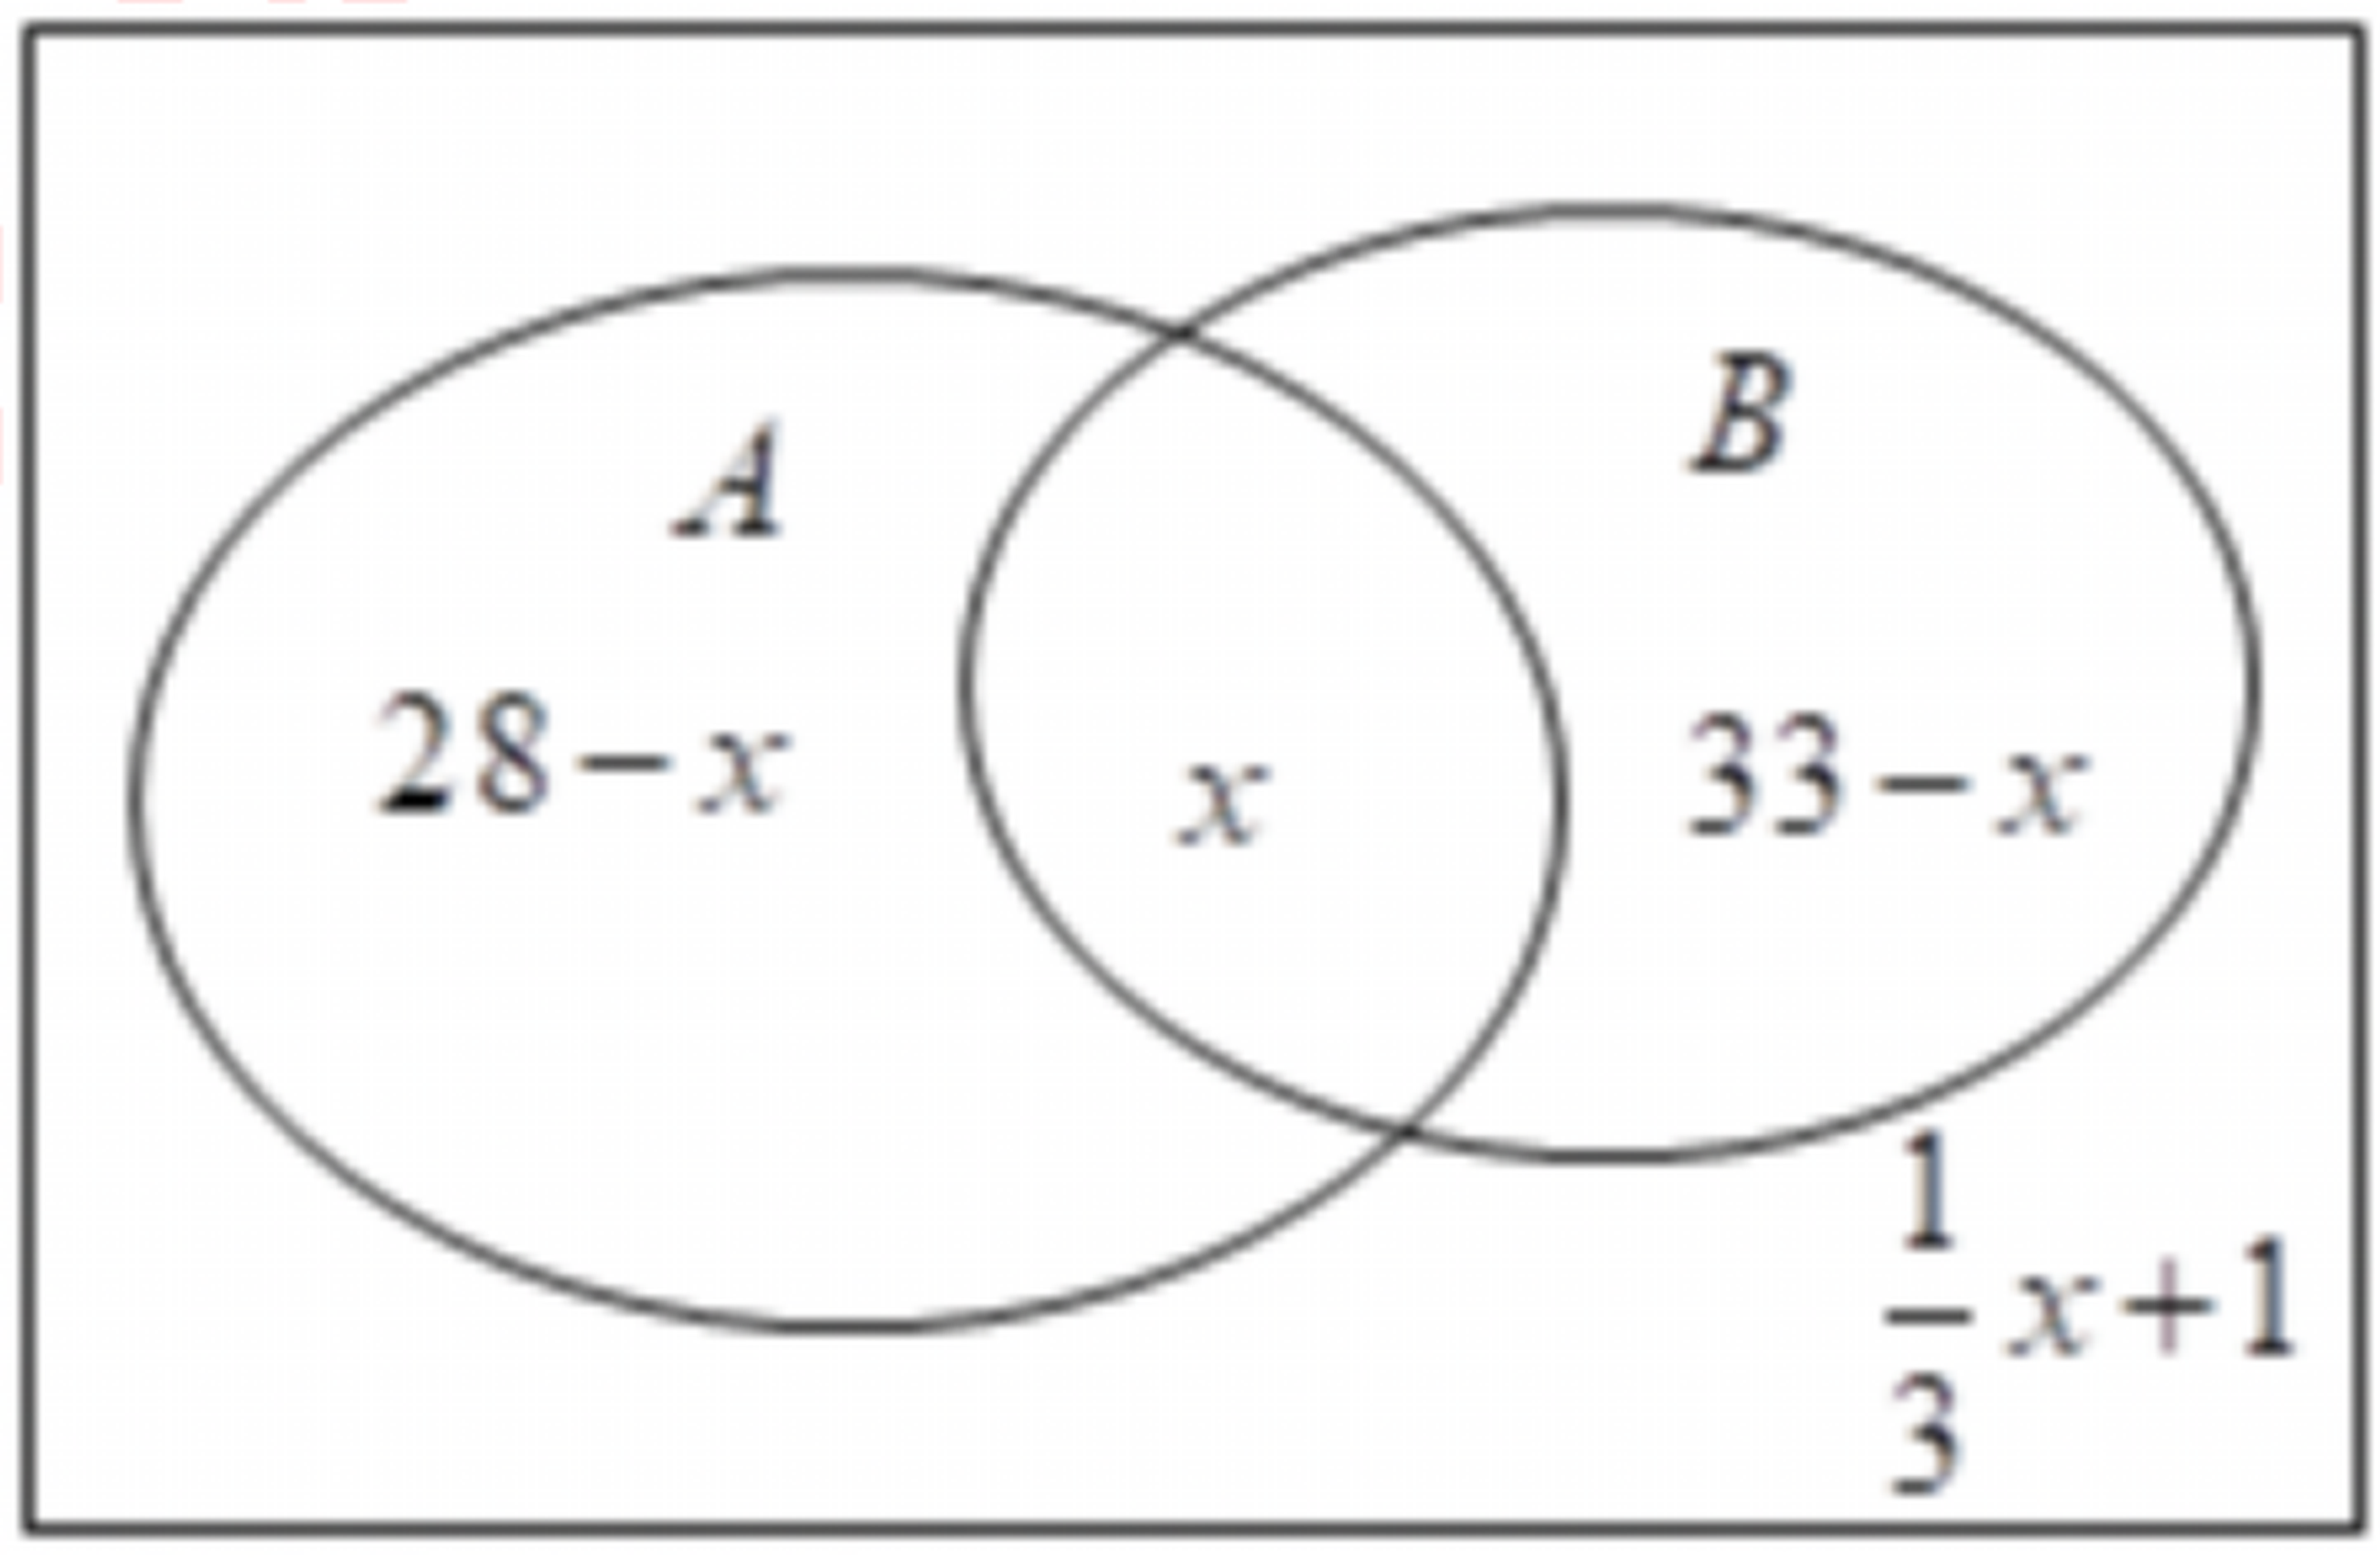
\includegraphics[width=0.42\textwidth]{figures/venn_AB_survey_50_x.png}
\end{center}
\step{则仅参加 $A$ 项的有 $(28-x)$ 人，仅参加 $B$ 项的有 $(33-x)$ 人，}
\step{$A$、$B$ 两项公益活动都不参加的有 $\left(\dfrac13x+1\right)$ 人，}
\step{由题意得 $x+(28-x)+(33-x)+\left(\dfrac13x+1\right)=50$，解得 $x=18$，}
\step{所以只参加 $A$ 项不参加 $B$ 项的有 $28-18=10$ 人.}
\solend
\fi

\item 设集合 $A=\{x\mid x^2-3x+2=0\}$，则满足 $A\cup B=\{0,1,2\}$ 的集合 $B$ 的个数是 \blankline[4.4em].

\ans{$4$}

\ifanswer
\solbegin
\step{$A=\{x\mid x^2-3x+2=0\}=\{x\mid x=1\text{ 或 }x=2\}=\{1,2\}$，}
\step{若 $A\cup B=\{0,1,2\}$，则 $0\in B$，}
\step{则 $B=\{0\},\{0,2\},\{1,0\},\{0,1,2\}$，共 $4$ 个.}
\solend
\fi

\item 已知全集 $U=\R$，集合 $A=\{x\mid x^2<4\}$，$B=\{y\mid y=x^2\}$，则图中阴影部分所表示的集合为 \blankline[4.4em].

\begin{center}
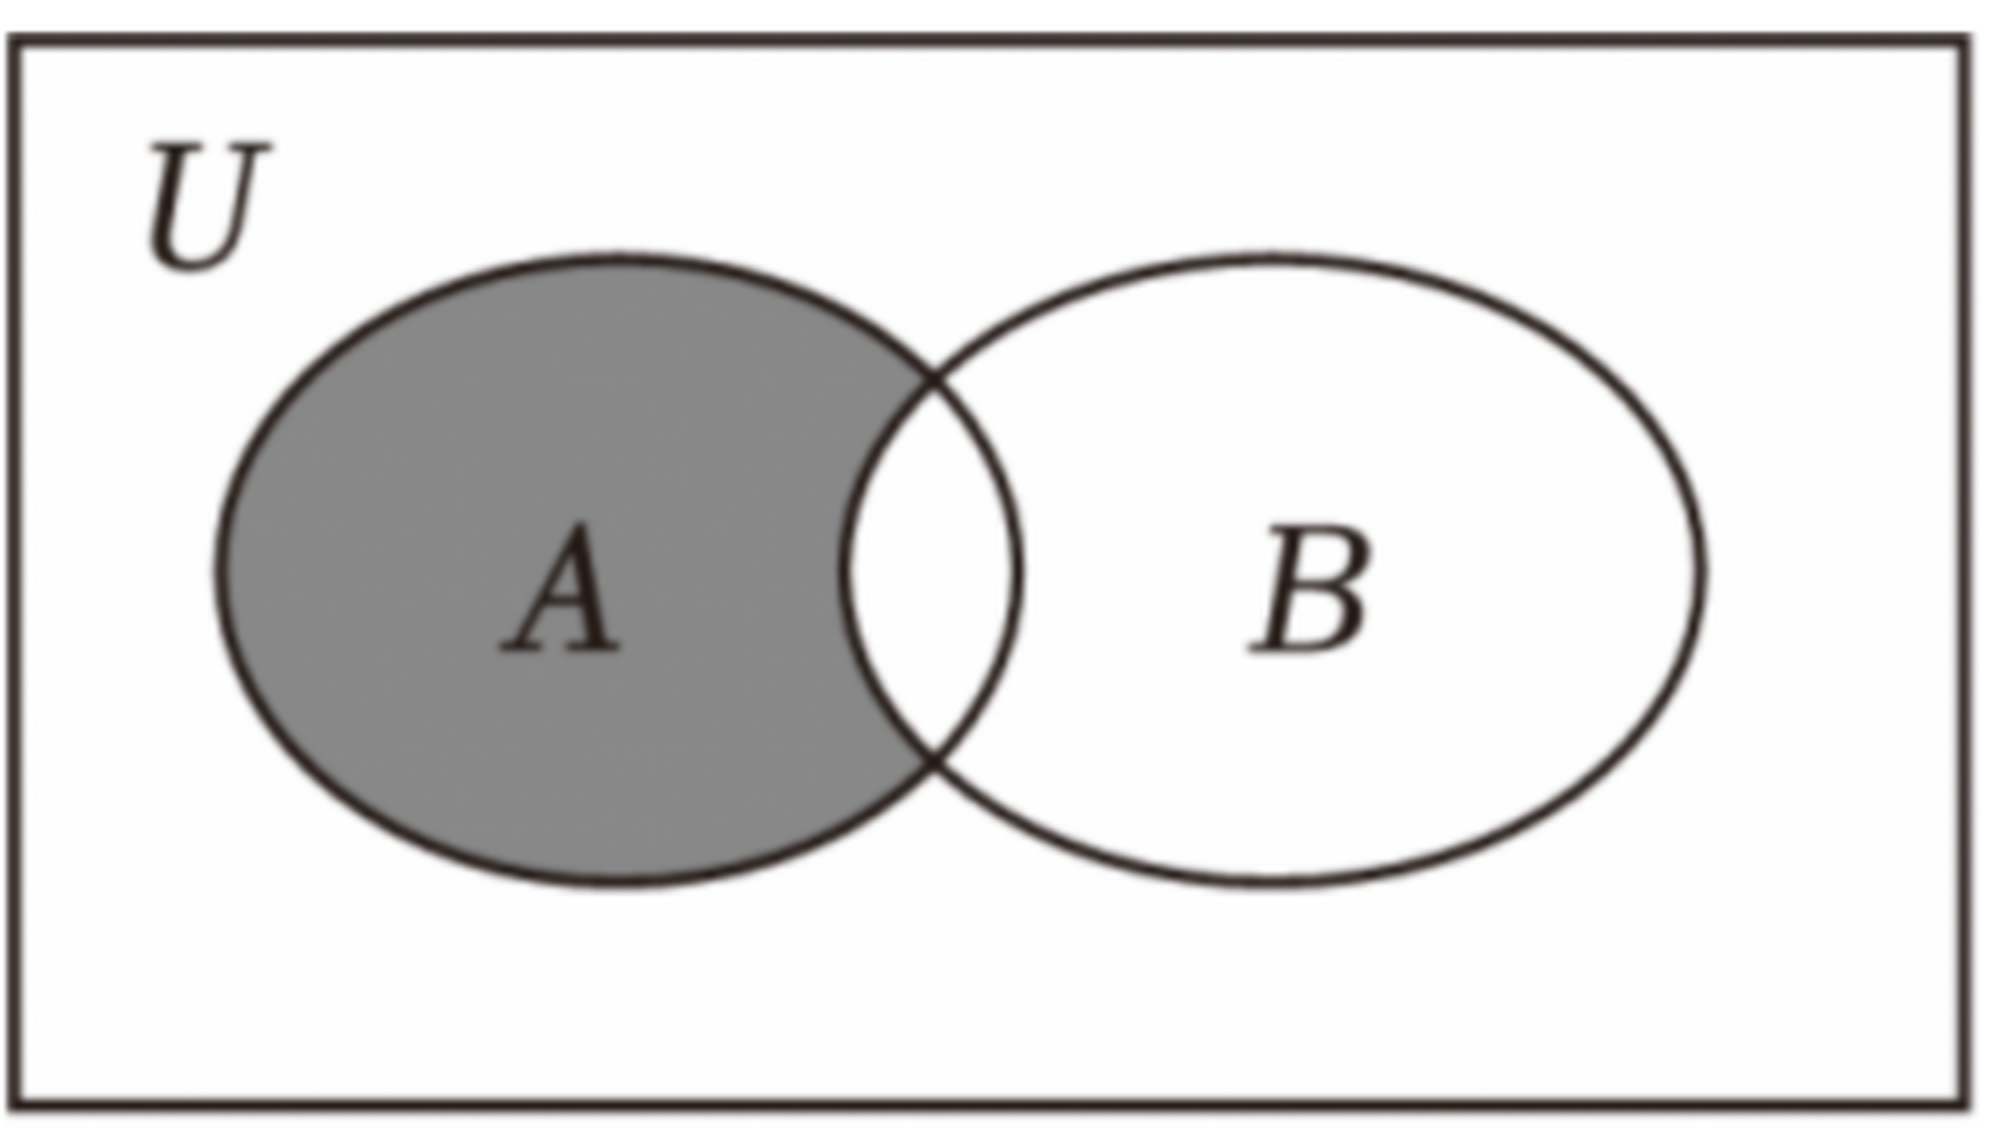
\includegraphics[width=0.34\textwidth]{figures/venn_A_shaded_U.png}
\end{center}

\ans{$A\cap\overline B=(-2,0)$}

\ifanswer
\solbegin
\step{集合 $A=\{x\mid x^2<4\}=(-2,2)$，$B=\{y\mid y=x^2\}=[0,+\infty)$，}
\step{图中阴影部分所表示的集合是 $A\cap\overline B=(-2,0)$.}
\solend
\fi

\item 如图所示，$M$、$P$、$S$ 是 $V$ 的三个子集，则阴影部分所表示的集合是 \blankline[5.4em].

\begin{center}
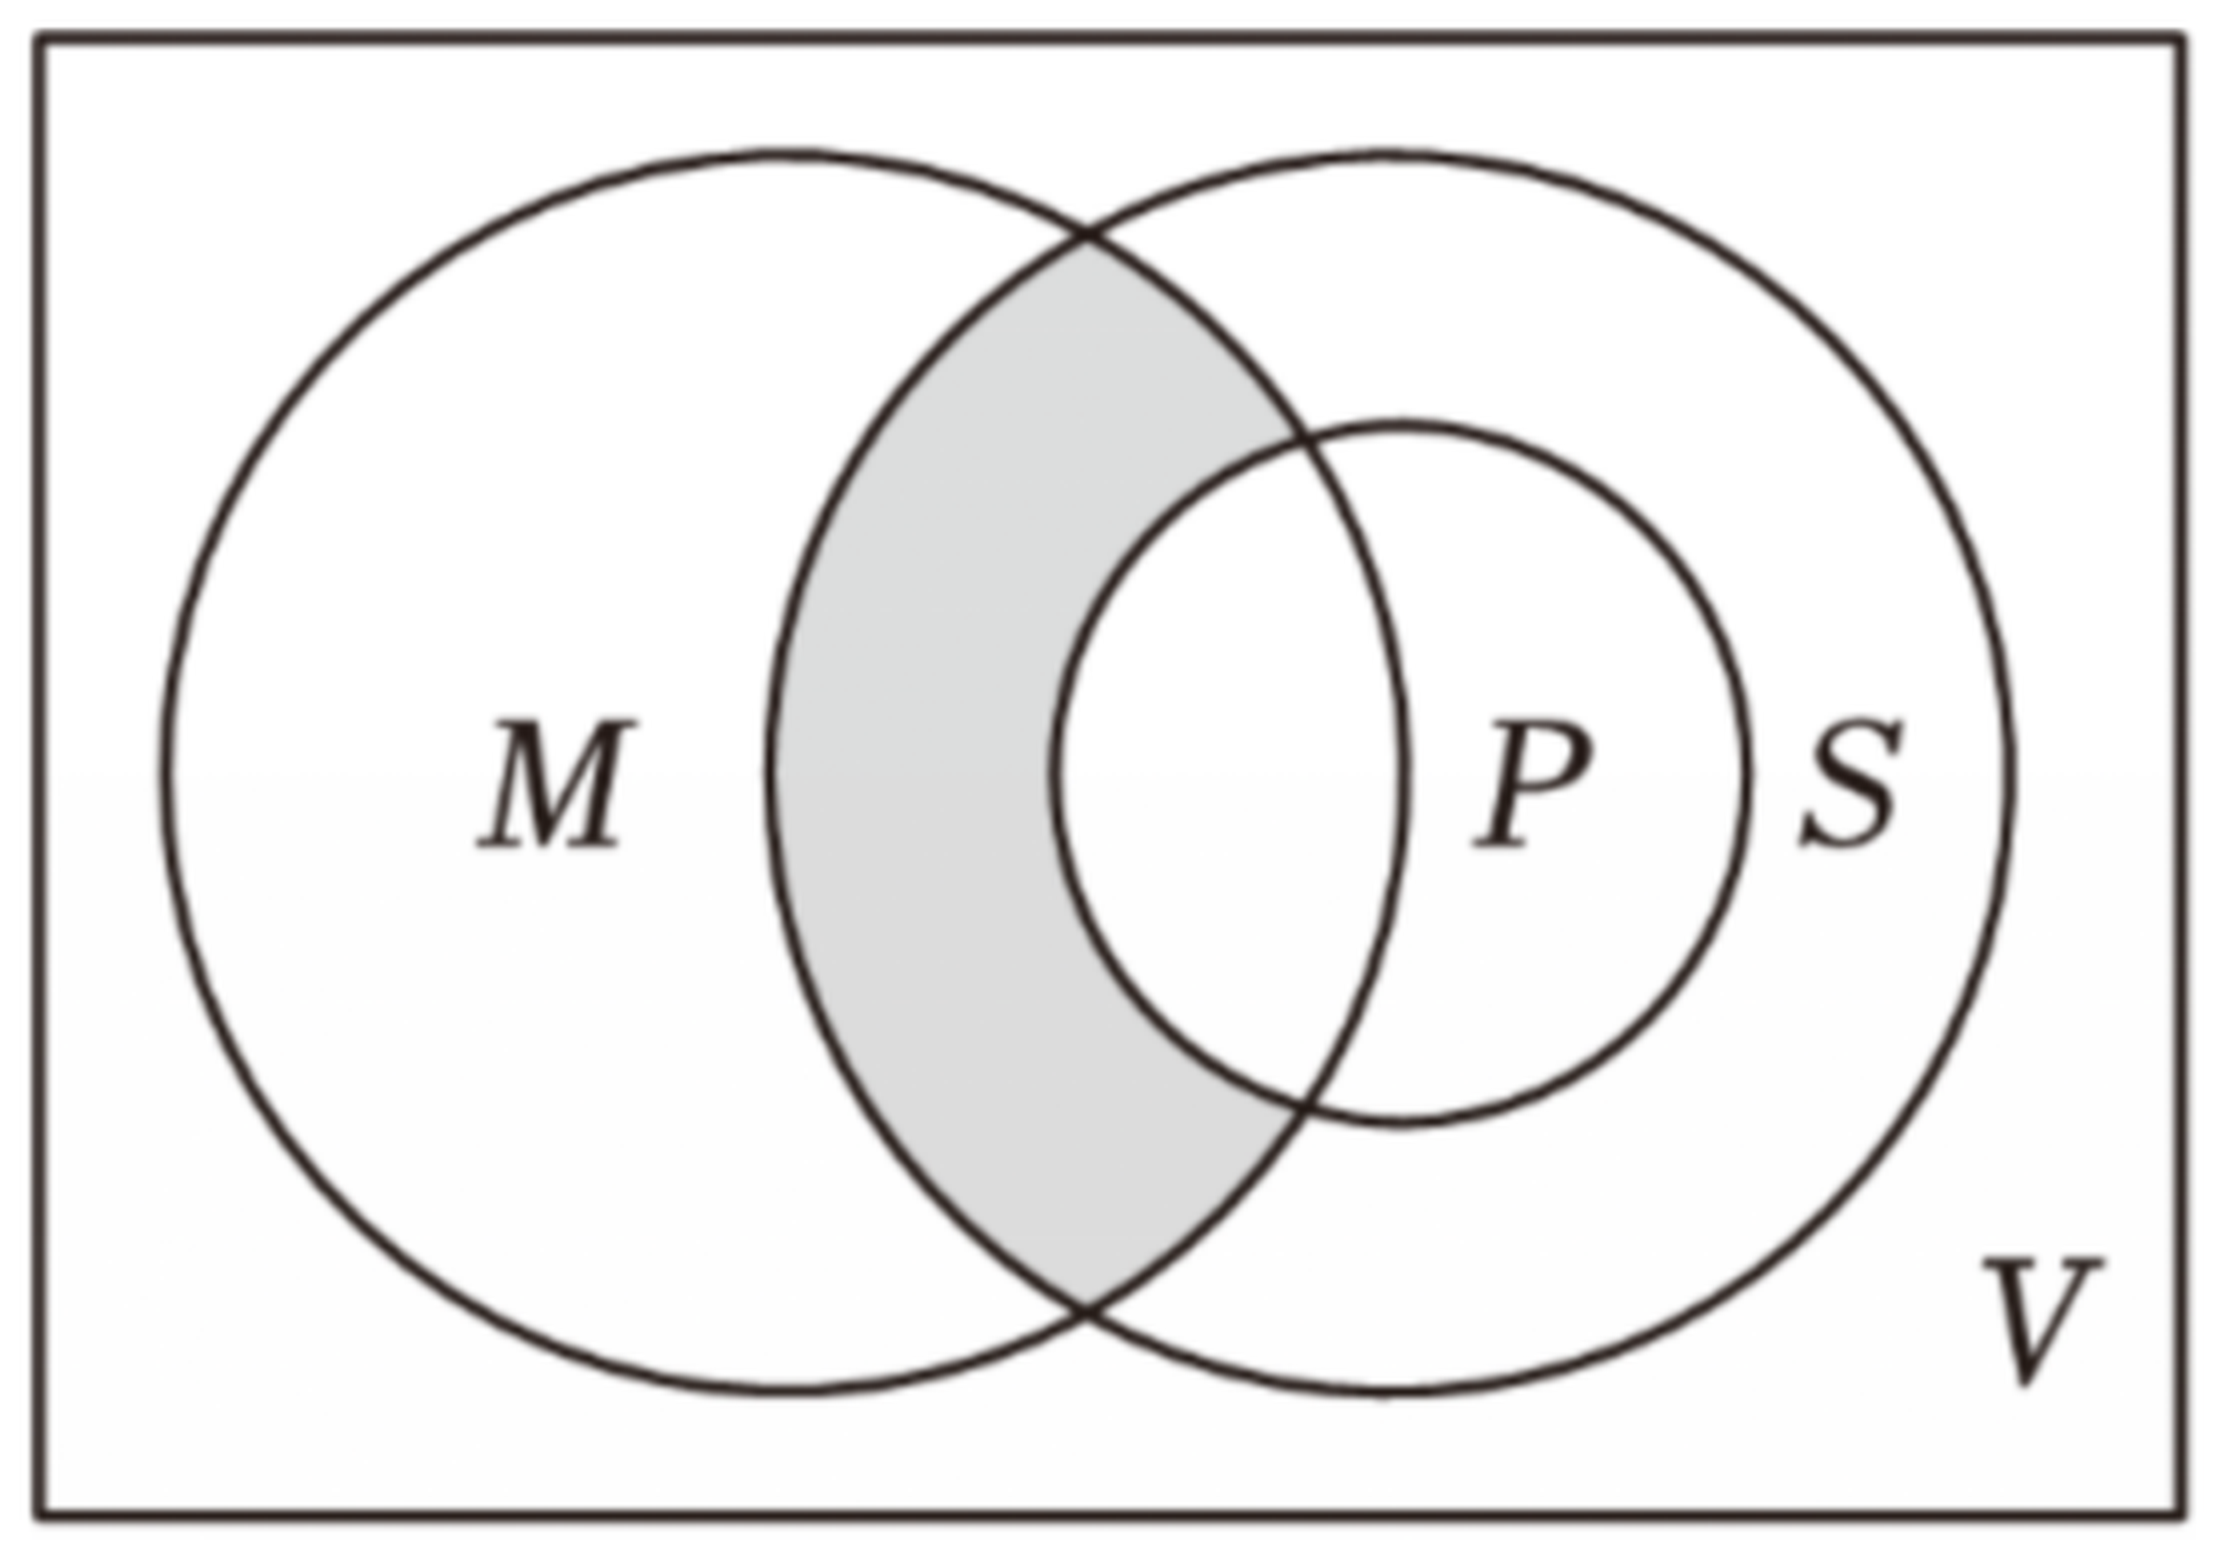
\includegraphics[width=0.38\textwidth]{figures/venn_MPS_V.png}
\end{center}

\ans{$(M\cap S)\cap(\complement_V P)$}

\item 下面六个关系式：① $\varnothing\subseteq\{a\}$；② $a\subseteq\{a\}$；③ $\{a\}\subseteq\{a\}$；④ $\{a\}\in\{a,b\}$；⑤ $a\in\{a,b,c\}$；⑥ $\varnothing\in\{a,b\}$；其中正确的是 \blankline[3.4em].

\ans{①③⑤}

\item 已知集合 $A=\{x\mid -1\le x\le a\}\ne\varnothing$，若 $\{y\mid y=x+1,x\in A\}=\{y\mid y=x^2,x\in A\}$，则实数 $a$ 值为 \blankline[4.4em].

\ans{$0$ 或 $\dfrac{1+\sqrt5}{2}$}

\ifanswer
\solbegin
\step{因为 $A=\{x\mid -1\le x\le a\}\ne\varnothing$，}
\step{所以 $\{y\mid y=x+1,x\in A\}=\{y\mid 0\le y\le a+1\}$，}
\step{$-1\le a\le1$ 时，$\{y\mid y=x^2,x\in A\}=\{y\mid 0\le y\le1\}$，}
\step{$a>1$ 时，$\{y\mid y=x^2,x\in A\}=\{y\mid 0\le y\le a^2\}$，}
\step{① $-1\le a\le1$ 时，$\{y\mid 0\le y\le a+1\}=\{y\mid 0\le y\le1\}$，则 $a+1=1$，解得 $a=0$；}
\step{② $a>1$ 时，$\{y\mid 0\le y\le a+1\}=\{y\mid 0\le y\le a^2\}$，则 $a^2=a+1$，解得 $a=\dfrac{1+\sqrt5}{2}$；}
\step{所以 $a=0$ 或 $\dfrac{1+\sqrt5}{2}$.}
\solend
\fi

\item 设集合 $A=\{(x,y)\mid x+y=22,x>0,y>0,x,y\text{ 均为质数}\}$ 的子集的个数为 \blankline[4.4em].

\ans{$32$}

\ifanswer
\solbegin
\step{集合 $A=\{(x,y)\mid x+y=22,x>0,y>0,x,y\text{ 均为质数}\}$}
\step{$=\{(3,19),(19,3),(5,17),(17,5),(11,11)\}$，则 $A$ 的子集的个数为 $2^5=32$.}
\solend
\fi

% 注：原卷本题题干印作「已知一个有四个数字元素的集合 $S$」；「数字元素」疑为「元素」之衍，
%     但原卷字形确为「数字」二字（已 3× 放大核对过），本稿照录，不代为改写。
\item 已知一个有四个数字元素的集合 $S$，$S$ 的所有子集的元素和（空集的元素和认为是 $0$）的总和为 $16192$，则 $S$ 的元素之和等于 \blankline[4.4em].

\ans{$2024$}

\ifanswer
\solbegin
\step{设 $S=\{a_1,a_2,a_3,a_4\}$，$S$ 的每个元素在所有子集中均出现 $2^3$ 次，}
\step{故 $(a_1+a_2+a_3+a_4)\cdot 2^3=16192$，所以 $a_1+a_2+a_3+a_4=2024$，}
\step{故 $S$ 的元素之和等于 $2024$.}
\solend
\fi

\item 设 $A$ 是非空数集，若对任意 $x$、$y\in A$，都有 $x+y\in A$、$xy\in A$，则称 $A$ 具有性质 $P$，给出以下命题：

①若 $A$ 具有性质 $P$，则 $A$ 可以是有限集；

②若 $A$ 具有性质 $P$，且 $A\ne\R$，则 $\overline A$ 具有性质 $P$；

③若 $A_1$、$A_2$ 具有性质 $P$，且 $A_1\cap A_2\ne\varnothing$，则 $A_1\cap A_2$ 具有性质 $P$；

④若 $A_1$、$A_2$ 具有性质 $P$，则 $A_1\cap A_2$ 具有性质 $P$.

其中所有真命题的序号是 \blankline[4.4em].

\ans{①③}

\ifanswer
\solbegin
\step{对于①，取集合 $A=\{0,1\}$ 具有性质 $P$，故 $A$ 可以是有限集，故①正确；}
\step{对于③，取 $x$、$y\in A_1\cap A_2$，则 $x\in A_1$，$x\in A_2$，$y\in A_1$，$y\in A_2$，}
\step{又 $A_1$、$A_2$ 具有性质 $P$，所以 $x+y\in A_1$，$xy\in A_1$，$x+y\in A_2$，$xy\in A_2$，}
\step{所以 $x+y\in A_1\cap A_2$，$xy\in A_1\cap A_2$，所以 $A_1\cap A_2$ 具有性质 $P$，故③正确；}
\step{对于④，取 $A_1=\{x\mid x=2k,k\in\Z\}$，$A_2=\{x\mid x=3k,k\in\Z\}$，$2\in A_1$，$3\in A_2$，}
\step{但 $2+3\notin A_1\cup A_2$，故④错误；}
\step{对于②，若 $A$ 具有性质 $P$，且 $A\ne\R$，假设 $\overline A$ 也具有性质 $P$，}
\step{设 $0\in A$，在 $\overline A$ 中任取一个 $x$，$x\ne0$，此时可证得 $-x\in A$，}
\step{否则若 $-x\in\overline A$，由于 $\overline A$ 也具有性质 $P$，则 $x+(-x)=0\in\overline A$，}
\step{与 $0\in A$ 矛盾，故 $-x\in A$，}
\step{由于 $A$ 具有性质 $P$，$\overline A$ 也具有性质 $P$，所以 $(-x)^2\in A$，$x^2\in\overline A$，}
\step{而 $(-x)^2=x^2$，这与 $A\cap\overline A=\varnothing$ 矛盾，}
\step{故当 $0\in A$ 且 $A$ 具有性质 $P$ 时，则 $\overline A$ 不具有性质 $P$，}
\step{同理当 $0\in\overline A$ 时，也可以类似推出矛盾，故②错误.}
\step{故正确的是①③.}
\solend
\fi

\item 已知 $S=\{1,2,3,4,5\}$，$A=\{1,2,5\}$，$T=\{t_1,t_2\}\subseteq S$，记 $A_1=\{x\mid x=a+t_1,a\in A,t_1\in T\}$，$A_2=\{x\mid x=b+t_2,b\in A,t_2\in T\}$，若 $A_1\cap A_2=\varnothing$，则集合 $T$ 为 \blankline[5.4em].

\ans{$T=\{1,3\}$ 或 $T=\{2,4\}$ 或 $T=\{3,5\}$}

\ifanswer
\solbegin
\step{若 $A_1\cap A_2=\varnothing$，即 $a+t_1\ne b+t_2$，则 $t_1-t_2\ne a-b$，其中 $a$、$b\in A$，}
\step{否则 $t_1+a=t_2+b$，$A_1\cap A_2\ne\varnothing$，}
\step{又 $S=\{1,2,3,4,5\}$，$A=\{1,2,5\}$，$T=\{t_1,t_2\}\subseteq S$，}
\step{$2-1=1$，$5-2=3$，$5-1=4$，则 $t_1$、$t_2$ 相差 $2$，}
\step{所以 $T=\{1,3\}$ 或 $T=\{2,4\}$ 或 $T=\{3,5\}$.}
\solend
\fi

\end{enumerate}

\bigsec{二、解答题}

\begin{enumerate}
\setcounter{enumi}{13}

\item 设集合 $P=\{1,2,3,m\}$，$Q=\{3,m^2\}$，且 $\overline P\cap Q=\varnothing$，求实数 $m$ 的值组成的集合.

\ans{$\{-1,0,\pm\sqrt2\}$}

\ansspace[5]

\ifanswer
\solbegin
\step{因为 $\overline P\cap Q=\varnothing$，所以 $Q\subseteq P$，所以 $m^2=1$ 或 $m^2=2$ 或 $m^2=m$，}
\step{考虑互异性，得 $m=-1$ 或 $m=\pm\sqrt2$ 或 $m=0$，}
\step{所以实数 $m$ 的值组成的集合为 $\{-1,0,\pm\sqrt2\}$.}
\solend
\fi

\item 若集合 $A=(-\infty,2]$，$B=\{x\mid kx+1<0,k\in\R\}$，$A\cap B=\varnothing$，求实数 $k$ 的取值范围.

\ans{$\left[-\dfrac12,0\right]$}

\ansspace[5]

\ifanswer
\solbegin
\step{若 $B=\varnothing$，则 $k=0$，符合题意，}
\step{若 $B\ne\varnothing$，当 $k>0$ 时，$B=\left(-\infty,-\dfrac1k\right)$，$A\cap B\ne\varnothing$，不合题意；}
\step{当 $k<0$ 时，$B=\left(-\dfrac1k,+\infty\right)$，由 $A\cap B=\varnothing$ 得 $-\dfrac1k\ge2$，即 $-\dfrac12\le k<0$，}
\step{故 $k$ 的取值范围是 $\left[-\dfrac12,0\right]$.}
\solend
\fi

\item 已知集合 $A=\{-4,2a-1,a^2\}$，$B=\{a-5,1-a,9\}$，分别求适合下列条件的 $a$ 的值.

% 两个小问不许与题干分家：试卷版第 2 页页末原本正好把 (1) 留在页底、(2) 翻到次页，
% 与 2026-09-15 修的三类难看切页同源，故在这里也加 \keepwithprev 守卫（三版都生效）。
\keepwithprev
（1）$9\in(A\cap B)$；

\keepwithprev
（2）$\{9\}=A\cap B$.

\ans{（1）$a=5$ 或 $a=-3$；（2）$a=-3$}

\ansspace[5]

\ifanswer
\solbegin
\stepm{（1）}{$9\in(A\cap B)$，所以 $9\in A$，}
\step{当 $2a-1=9$ 时，$a=5$，当 $a^2=9$ 时，即 $a=\pm3$，}
% 注：原卷此句结论印作「所以 $a$ 的值为 $5\backslash-3$」——「\」应是顿号之误，
%     本稿照录原卷字形（见文件头「原卷存疑」②）；按文意即 $a=5$ 或 $a=-3$。
\step{当 $a=3$ 时，$a-5=1-a$ 舍去，所以 $a$ 的值为 $5\backslash-3$.}
\stepm{（2）}{结合（1）的结论：}
\step{当 $2a-1=9$ 即 $a=5$ 时，$1-a=-4$，$\{9\}\ne(A\cap B)$，}
\step{当 $a^2=9$ 时，即 $a=\pm3$，当 $a=3$ 时，$a-5=1-a$ 舍去，}
\step{所以 $a$ 的值为 $-3$.}
\solend
\fi

\item 已知集合 $M=\{a,ab,a-b\}$，$N=\{0,|a|,b\}$，且 $M=N$，求实数 $a$、$b$ 的值.

\ans{$a=b=-1$}

\ansspace[5]

\ifanswer
\solbegin
\step{由集合元素的互异性，得 $a\ne0$，且 $b\ne0$，所以 $a-b=0$，即 $a=b$，}
\step{所以 $ab=|a|$，又由 $|a|\ne b=a$，得 $a<0$，故 $a=b=-1$.}
\solend
\fi

\item 已知集合 $A=\{x\mid -2<x<7\}$，$B=\{x\mid m+1\le x\le 2m-1\}$.

\keepwithprev
（1）当 $m=4$ 时，求 $A\cap B$、$A\cup B$；

\keepwithprev
（2）若 $A\cap B=B$，求实数 $m$ 的取值范围.

\ans{（1）$A\cap B=[5,7)$，$A\cup B=(-2,7]$；（2）$(-\infty,4)$}

\ansspace[5]

\ifanswer
\solbegin
\stepm{（1）}{当 $m=4$ 时，得集合 $A=\{x\mid -2<x<7\}$，$B=\{x\mid 5\le x\le7\}$，}
\step{得 $A\cap B=[5,7)$，$A\cup B=(-2,7]$.}
\stepm{（2）}{由 $A\cap B=B$ 得 $B\subseteq A$，}
\step{①当 $B=\varnothing$ 时，得 $m+1>2m-1$，解得 $m<2$；}
\step{②当 $B\ne\varnothing$ 时，得 $\begin{cases}m+1>-2\\ 2m-1<7\\ m+1\le2m-1\end{cases}$，解得 $2\le m<4$；}
\step{综上，实数 $m$ 的取值范围是 $(-\infty,4)$.}
\solend
\fi

\item 若集合 $A=\{x\mid x^2+5x-6=0\}$，$B=\{x\mid x^2+2(m+1)x+m^2-3=0\}$.

\keepwithprev
（1）当 $m=0$ 时，求集合 $A\cup B$；

\keepwithprev
（2）若 $A\cap B=B$，求实数 $m$ 的取值范围.

\ans{（1）$A\cup B=\{1,-6,-3\}$；（2）$\{m\mid m\le-2\}$}

\ansspace[5]

\ifanswer
\solbegin
\stepm{（1）}{由题意得，集合 $A=\{x\mid x^2+5x-6=0\}=\{1,-6\}$，}
\step{当 $m=0$ 时，$B=\{x\mid x^2+2x-3=0\}=\{1,-3\}$，}
\step{所以 $A\cup B=\{1,-6,-3\}$；}
\stepm{（2）}{由（1）得集合 $A=\{1,-6\}$，$B=\{x\mid x^2+2(m+1)x+m^2-3=0\}$，}
\step{若 $A\cap B=B$ 得 $B\subseteq A$，所以 $B=\varnothing$ 或 $\{-6\}$ 或 $\{1\}$ 或 $\{1,-6\}$，}
\step{当 $B=\varnothing$ 时，$\Delta=4(m+1)^2-4(m^2-3)<0$，解得 $m<-2$，}
\step{当 $B=\{-6\}$ 时，则 $\begin{cases}\Delta=4(m+1)^2-4(m^2-3)=0\\ 36-12(m+1)+m^2-3=0\end{cases}$，无解，}
\step{当 $B=\{1\}$ 时，则 $\begin{cases}\Delta=4(m+1)^2-4(m^2-3)=0\\ 1+2(m+1)+m^2-3=0\end{cases}$，解得 $m=-2$，}
\step{当 $B=\{1,-6\}$ 时，则 $\begin{cases}\Delta=4(m+1)^2-4(m^2-3)>0\\ 1+(-6)=-2(m+1)\\ 1\times(-6)=m^2-3\end{cases}$，无解，}
\step{综上所述，实数 $m$ 的取值范围为 $\{m\mid m\le-2\}$.}
\solend
\fi

% 压轴题：其后已无内容，故作答区全用可丢弃胶水（\ansspace*），并在题目前先量一下版面。
\ansneed{8cm}
\item 对于点集 $A=\{(x,y)\mid x=m,y=-3x+2,m\in\N,m\ge1\}$，$B=\{(x,y)\mid x=n,y=a(x^2-x+1),n\in\N,n\ge1\}$，是否存在非零整数 $a$，使得 $A\cap B\ne\varnothing$？

\ans{$a=-1$}

\ansspace*[10]

\ifanswer
\solbegin
\step{当 $A\cap B\ne\varnothing$ 时，$-3x+2=a(x^2-x+1)$，}
\step{$ax^2+(3-a)x+a-2=0$ ①有正整数解，}
\step{所以 $\Delta=(3-a)^2-4a(a-2)=-3a^2+2a+9$ 是平方数，}
\step{所以 $3a^2-2a-9\le0$，$\dfrac{1-2\sqrt7}{3}\le a\le\dfrac{1+2\sqrt7}{3}$，$a\ne0$，$a\in\Z$，}
\step{所以 $a=\pm1$ 或 $a=2$，}
\step{$a=-1$ 时 $\Delta=4$，这时①变为 $-x^2+4x-3=0$，解得 $x_1=1$，$x_2=3$，}
\step{$A\cap B=\{(1,-1),(3,-7)\}$.}
\step{$a=1$ 时 $\Delta=8$，不是平方数.}
\step{$a=2$ 时 $\Delta=1$，这时①变为 $2x^2+x=0$，没有正整数解.}
\step{所以 $a=-1$.}
\solend
\fi

\end{enumerate}

\end{document}
"
%
% 原始材料是微信公众号图文（公众号「魔都数学加油站」，作者署名「破晓」，
% 原文链接 https://mp.weixin.qq.com/s/tHqWSV1StO5SHSXXQ4jeUA），正文为 6 张 PNG 页；
% 原文本身就是一份**讲评版**——题目下方直接印出【答案】或【解析】。本稿把答案与解析
% 移到答案版，试卷版即一张干净的空卷；试题文字、答案与解析均照原卷录入。
%
% 与原卷的排版差异（均已在 README「说明」中交代）：
%   ① 原文自**第 3 题**起（第 1、2 题未在该文发布），源码里以 \setcounter{enumi}{2} 起编；
%      全卷只有「一、填空题」「二、解答题」两节，无选择题；
%   ② 原卷本就印有两个分节标题（已在原图上逐页放大核对过），本稿照原卷分节，只把标题改排
%      成全稿统一的「大节标题」样式；
%   ③ 原卷的实数集、整数集、自然数集符号作正体 $R$、$Z$、$N$（第 15 题作粗体 $\mathbf{R}$，
%      第 20 题有 $N$ 与斜体 $Z$），本稿按全稿惯例统一写作 $\R$、$\Z$、$\N$；
%   ④ 第 4 题的韦恩图在原卷里印在【解析】右侧（题干并无「如图」二字），故本稿把该图放进
%      答案版的解析块内（`figures/venn_AB_survey_50_x.png`）；第 6、7 题的韦恩图是**题干图**
%      （题干作「图中阴影部分所表示的集合」），两版都排（`figures/venn_A_shaded_U.png`、
%      `figures/venn_MPS_V.png`）。三张图都取自原卷截图、4× LANCZOS 放大，不用 TikZ 手绘；
%   ⑤ 本卷也是「讲评版」，解析按全稿统一的 \solbegin/\step 分步重排（原卷为连续段落），
%      分步不改一字，只断句、断行；
%   ⑥ 标题前缀照**原卷**作「2026--2027 年…」（原卷标题即作「2026-2027年延安中学高一上周末
%      作业 2」）。同校的 高一06 作「学年度」——那是 高一02—高一09 那一批入库时统一改的；
%      后续入库的卷（高一10—高一17 与本卷）一律照原卷保留「年」，未强改，故同校两卷前缀不同。
%
% 原卷存疑两处（已逐处放大到能看清字形后核对，本稿照录并加注，见各题下的 `%` 注）：
%   （另有第三处「第 12 题【解析】末句」原先记作存疑，2026-09-26 第二轮核对放大后发现
%     原卷印的是「$0\in\overline A$」——A 上确有横杠，是本稿当初漏抄了 $\overline{}$；
%     已按原卷补回，故该条从存疑清单里删去，不计为原卷问题。）
%   ① 第 11 题题干印作「已知一个有四个数字元素的集合 $S$」，「数字元素」疑为「元素」之衍；
%   ② 第 16 题 (1) 结论印作「$a$ 的值为 $5\backslash-3$」，其中的「\」应是顿号之误
%      （由 (2) 的结论「$a$ 的值为 $-3$」可反推，(1) 的答案是 $5$ 或 $-3$）；

% 本篇在公众号「魔都数学加油站」连载里的编号是「27学年高一19」，本地编号与之对齐（高一19）；
% 对应关系见 README「与公众号连载号的对照表」。
\documentclass[a4paper,11pt]{article}
\usepackage{common}

\begin{document}

\examtitlest{2026--2027 年延安中学高一上周末作业 2}{集合与常用逻辑用语}

\bigsec{一、填空题}

\begin{enumerate}
% 原卷填空题从第 3 题起（1、2 未在该文中发布），须与解答题的 \setcounter{enumi}{13} 对齐
\setcounter{enumi}{2}
\item 已知全集 $U=\{1,2,3,4,5\}$，$M=\{1,2\}$，$P=\{1,3,5\}$，则 $M\cap\overline P=$ \blankline[4.4em].

\ans{$\{2\}$}

\item 某公司共有 $50$ 人，此次组织参加社会公益活动，其中参加 $A$ 项公益活动的有 $28$ 人，参加 $B$ 项公益活动的有 $33$ 人，且 $A$、$B$ 两项公益活动都不参加的人数比都参加的人数的三分之一多 $1$ 人，则只参加 $A$ 项不参加 $B$ 项的人数是 \blankline[4.4em].

\ans{$10$}

\ifanswer
\solbegin
\step{如图所示，设 $A$、$B$ 两项公益活动都参加的有 $x$ 人，}
\begin{center}
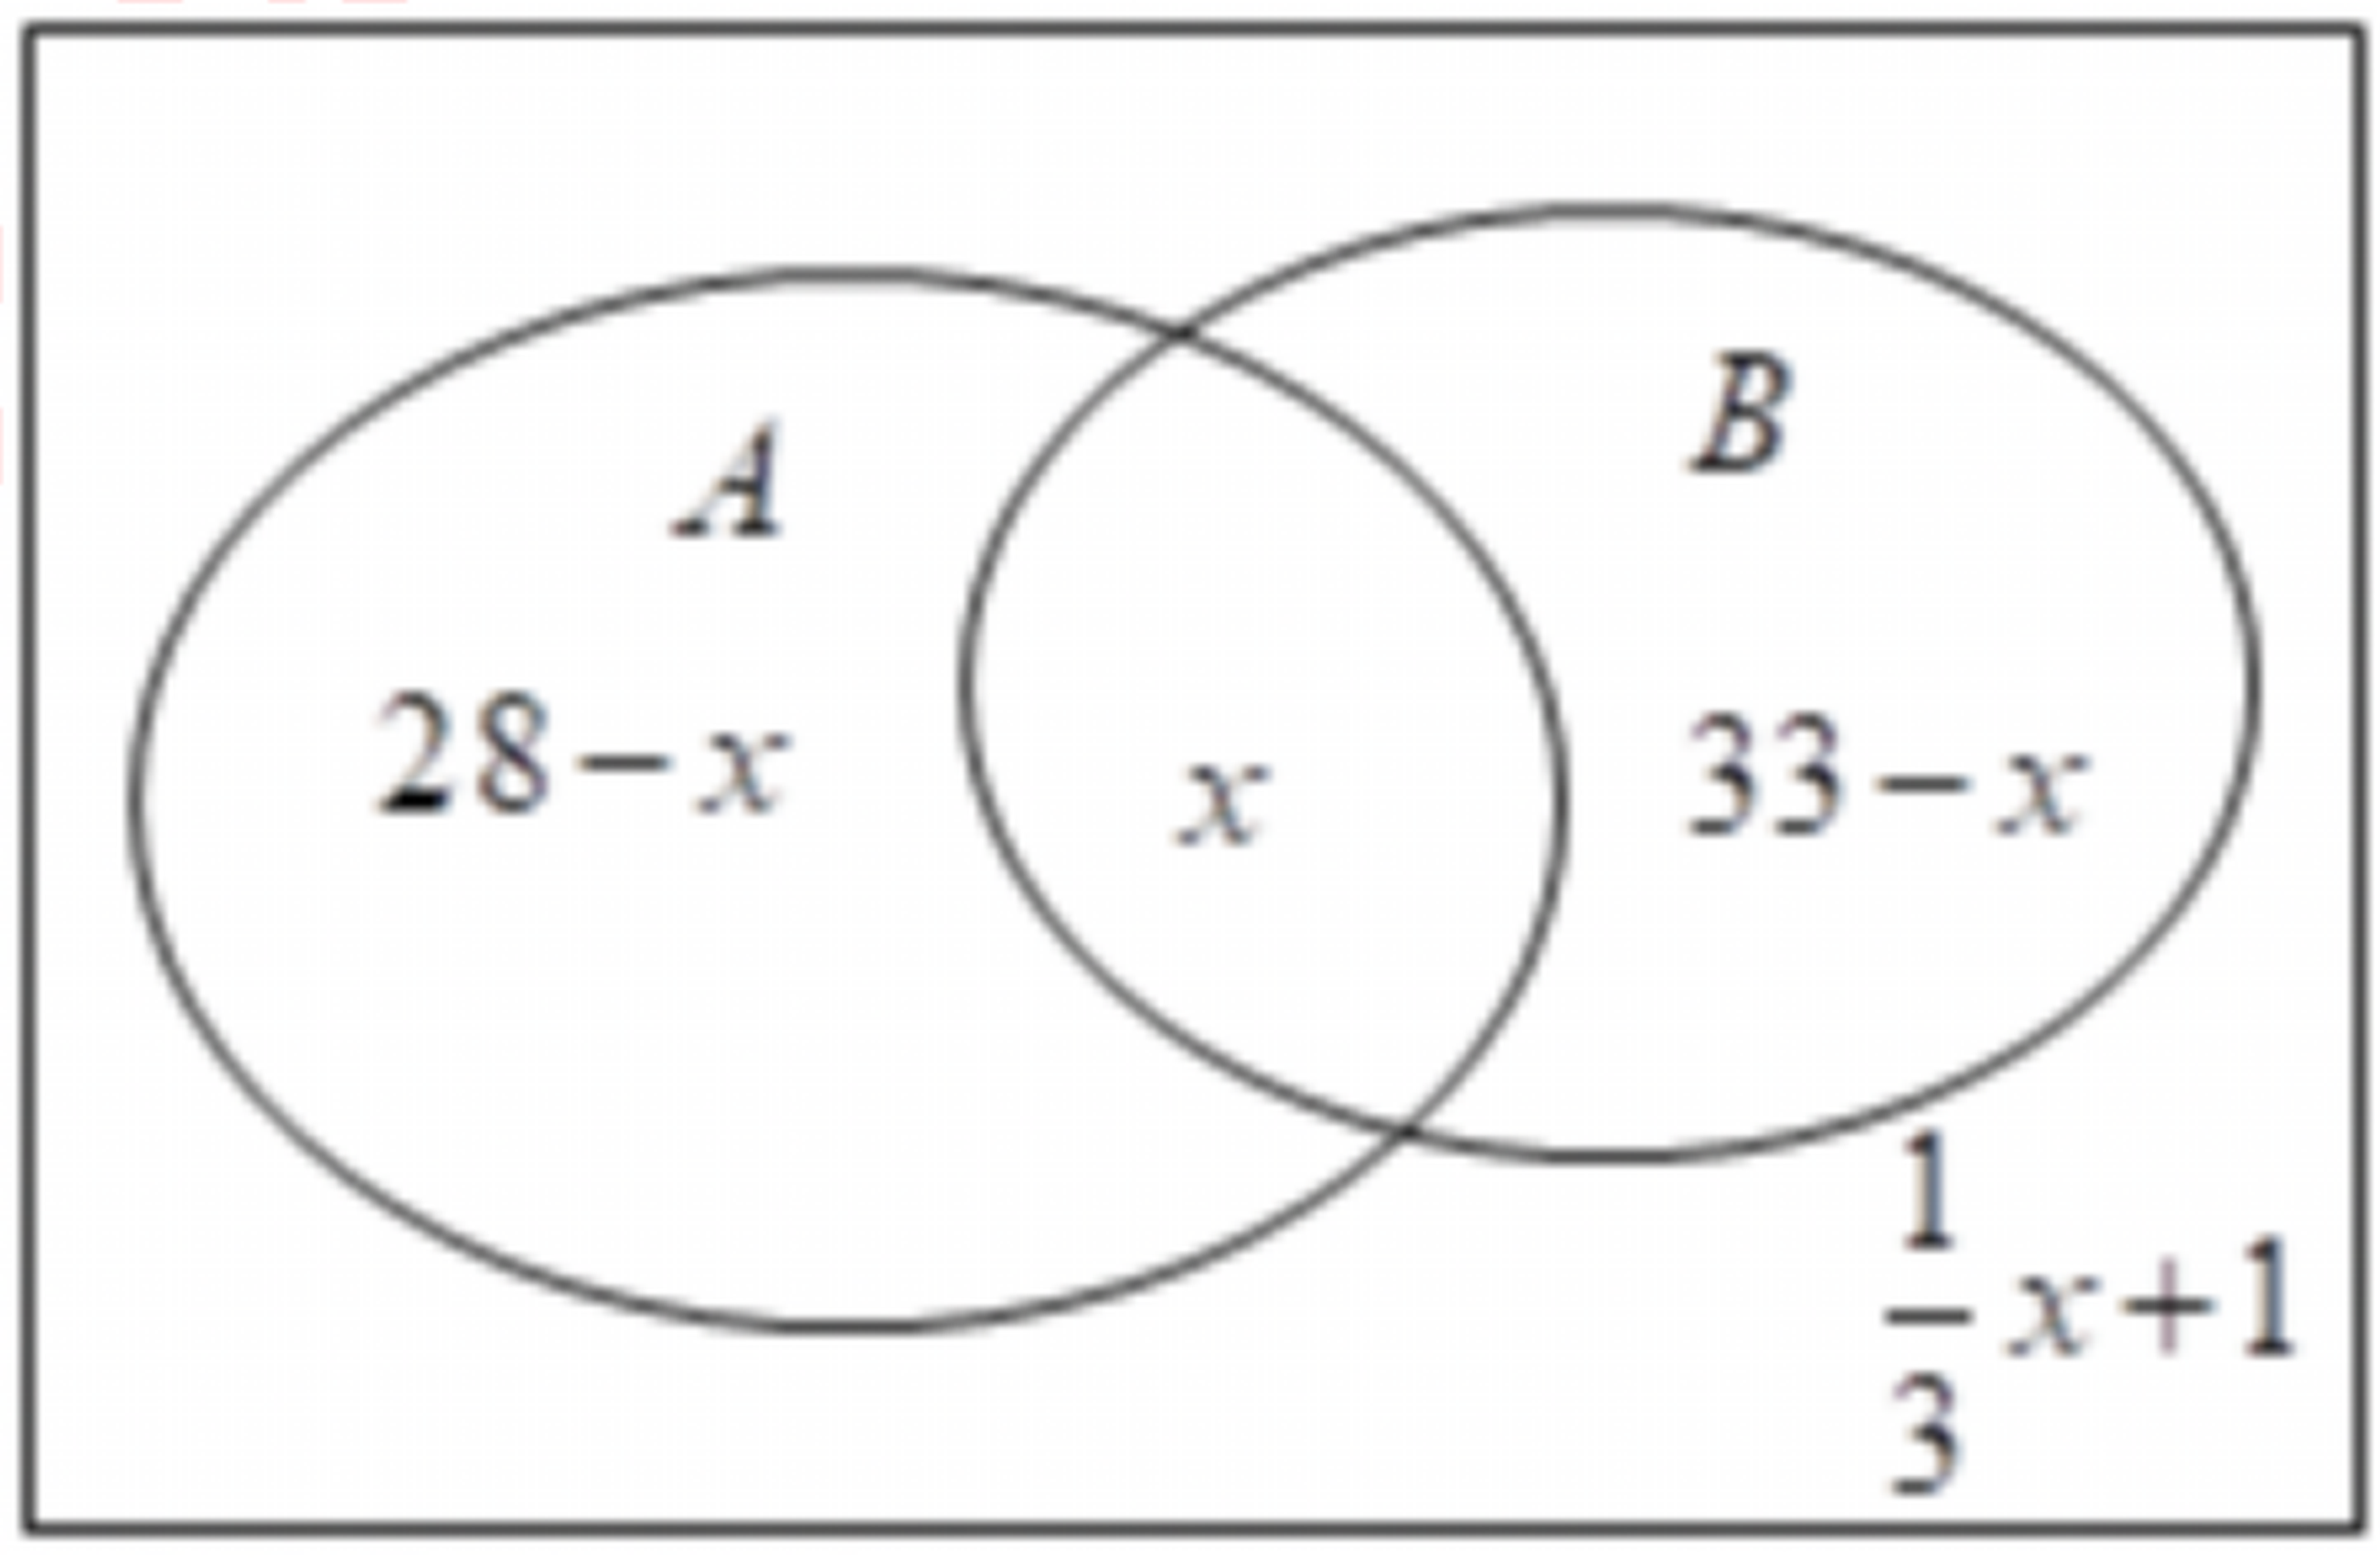
\includegraphics[width=0.42\textwidth]{figures/venn_AB_survey_50_x.png}
\end{center}
\step{则仅参加 $A$ 项的有 $(28-x)$ 人，仅参加 $B$ 项的有 $(33-x)$ 人，}
\step{$A$、$B$ 两项公益活动都不参加的有 $\left(\dfrac13x+1\right)$ 人，}
\step{由题意得 $x+(28-x)+(33-x)+\left(\dfrac13x+1\right)=50$，解得 $x=18$，}
\step{所以只参加 $A$ 项不参加 $B$ 项的有 $28-18=10$ 人.}
\solend
\fi

\item 设集合 $A=\{x\mid x^2-3x+2=0\}$，则满足 $A\cup B=\{0,1,2\}$ 的集合 $B$ 的个数是 \blankline[4.4em].

\ans{$4$}

\ifanswer
\solbegin
\step{$A=\{x\mid x^2-3x+2=0\}=\{x\mid x=1\text{ 或 }x=2\}=\{1,2\}$，}
\step{若 $A\cup B=\{0,1,2\}$，则 $0\in B$，}
\step{则 $B=\{0\},\{0,2\},\{1,0\},\{0,1,2\}$，共 $4$ 个.}
\solend
\fi

\item 已知全集 $U=\R$，集合 $A=\{x\mid x^2<4\}$，$B=\{y\mid y=x^2\}$，则图中阴影部分所表示的集合为 \blankline[4.4em].

\begin{center}
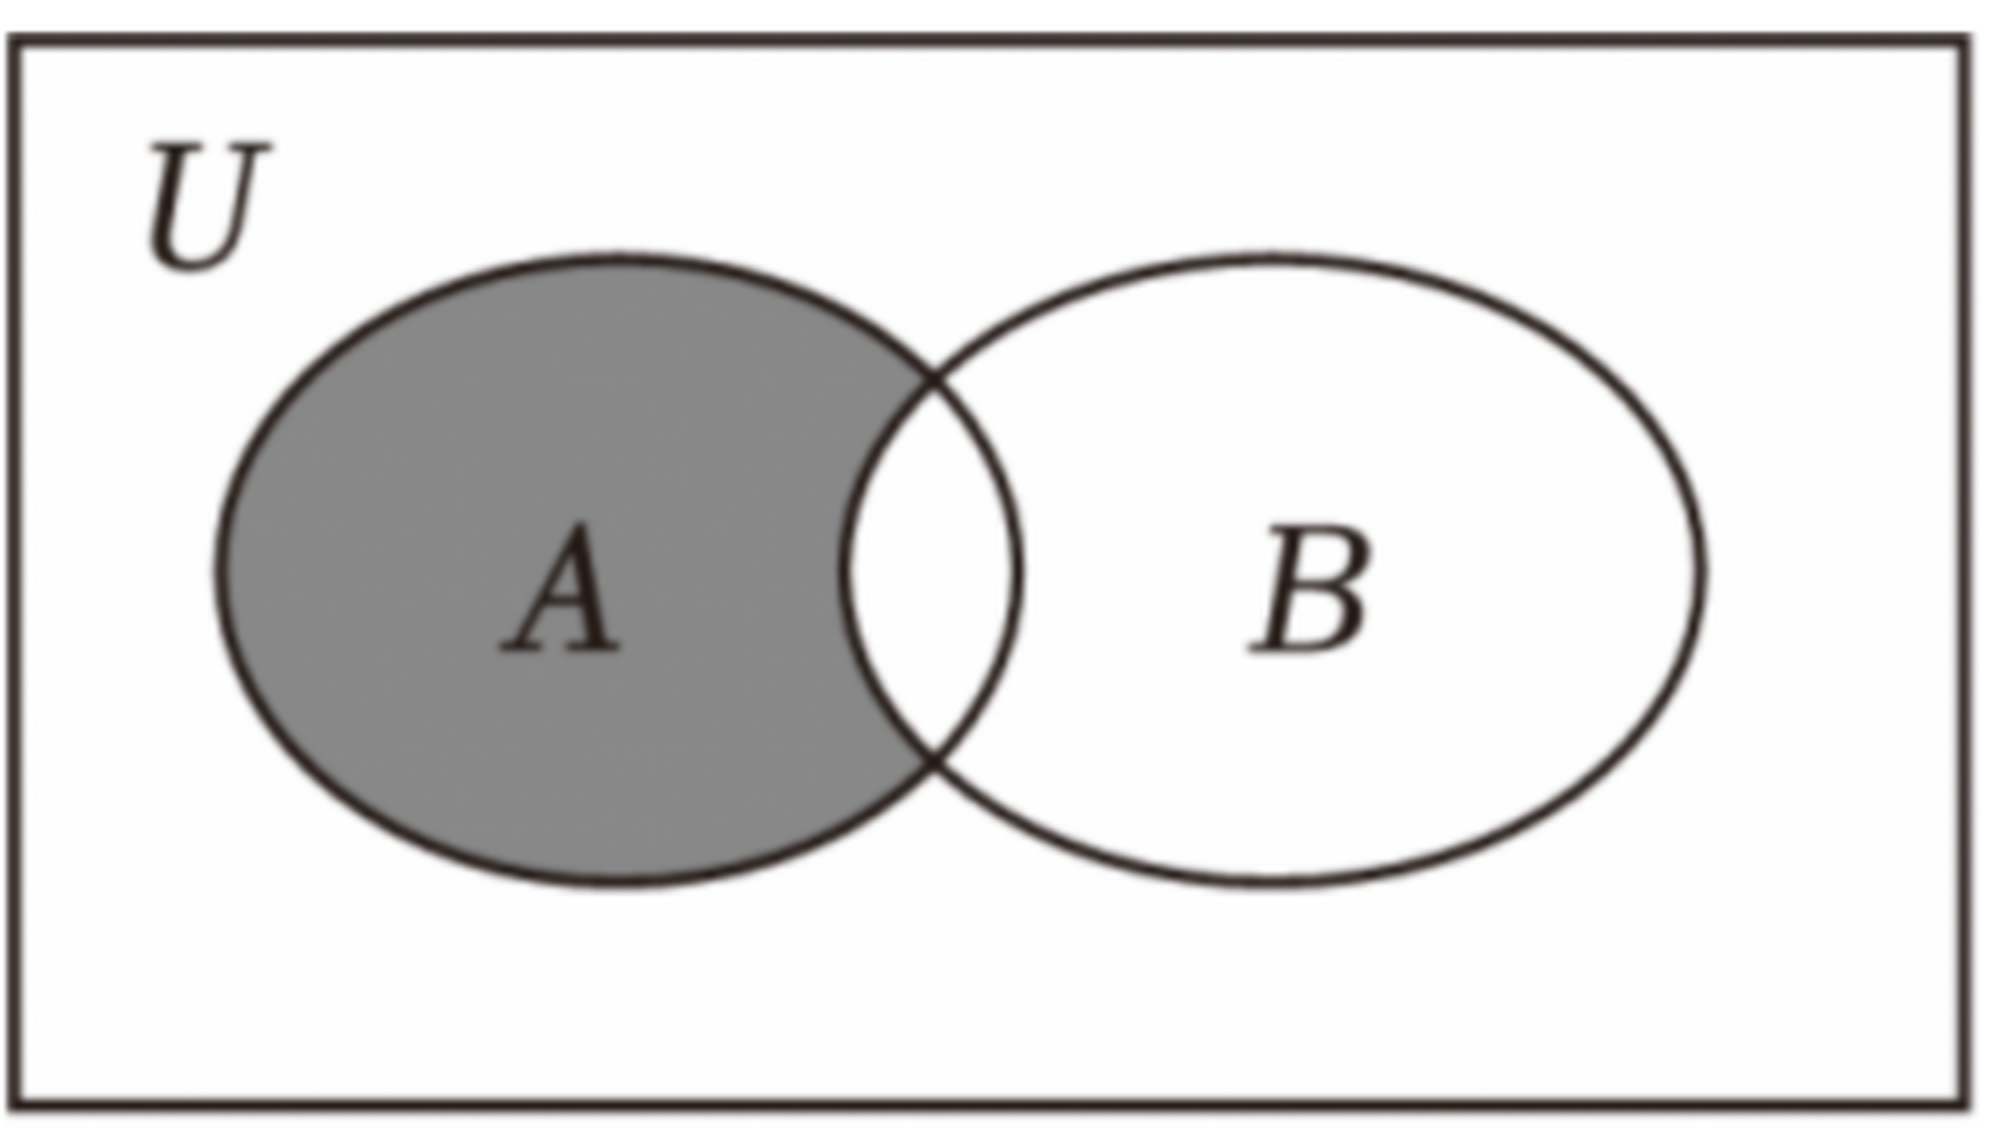
\includegraphics[width=0.34\textwidth]{figures/venn_A_shaded_U.png}
\end{center}

\ans{$A\cap\overline B=(-2,0)$}

\ifanswer
\solbegin
\step{集合 $A=\{x\mid x^2<4\}=(-2,2)$，$B=\{y\mid y=x^2\}=[0,+\infty)$，}
\step{图中阴影部分所表示的集合是 $A\cap\overline B=(-2,0)$.}
\solend
\fi

\item 如图所示，$M$、$P$、$S$ 是 $V$ 的三个子集，则阴影部分所表示的集合是 \blankline[5.4em].

\begin{center}
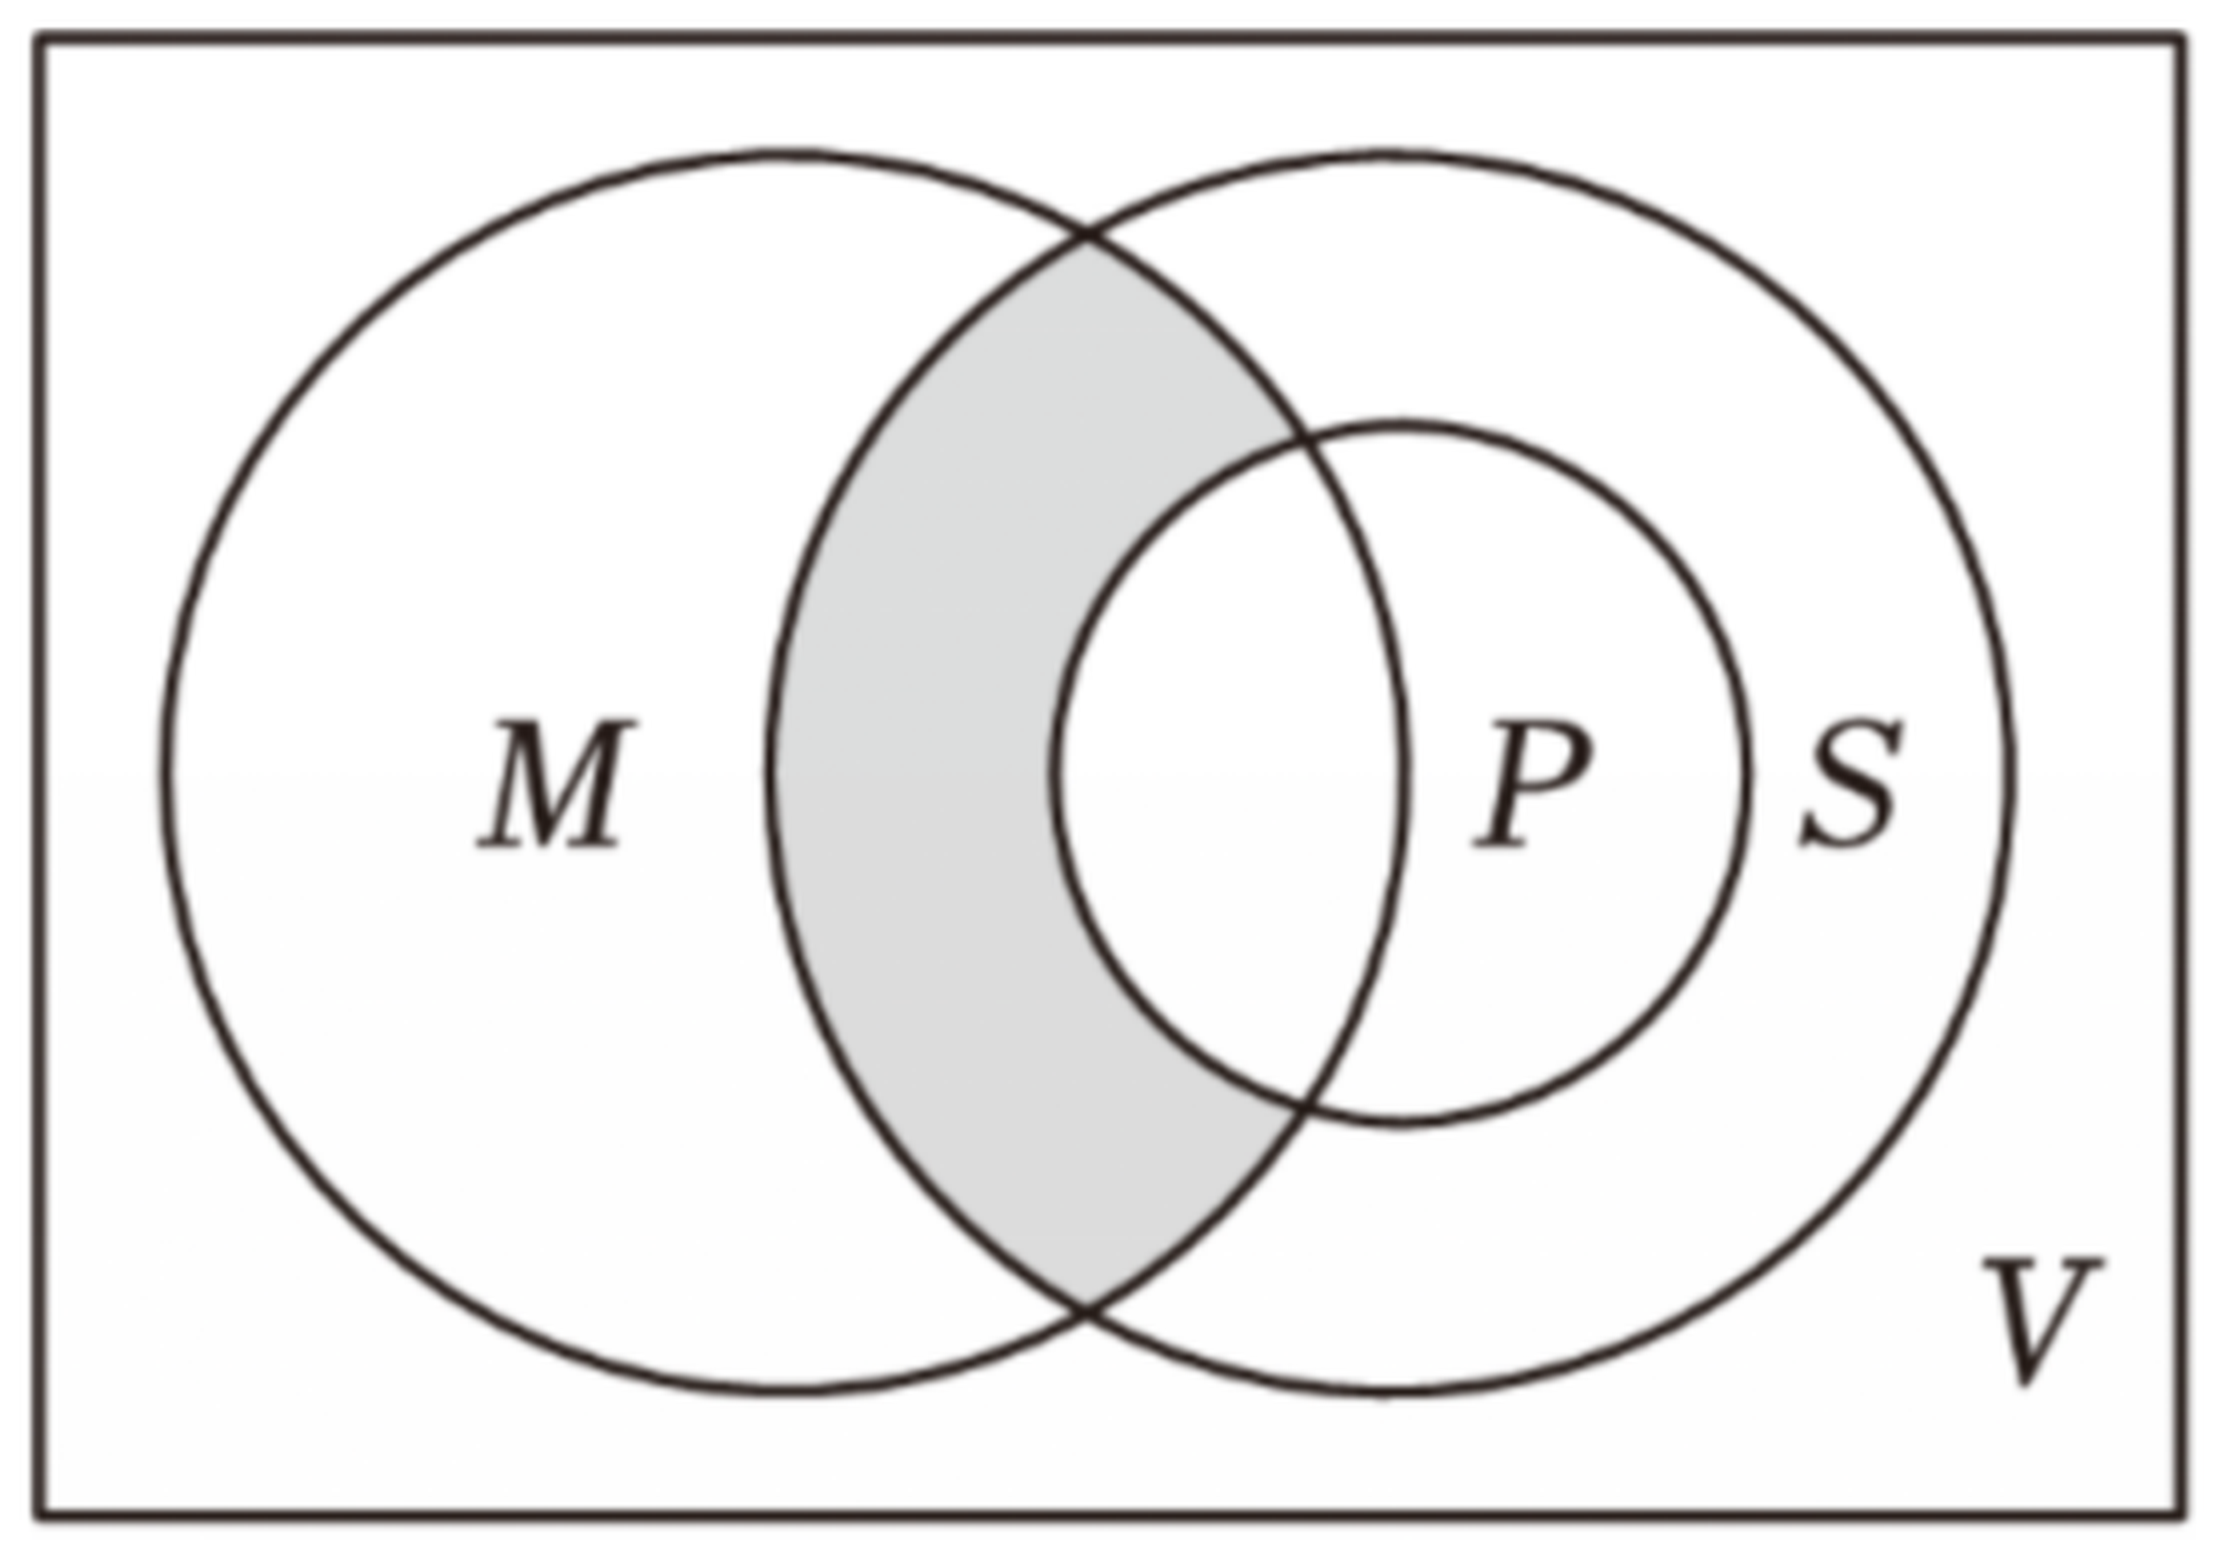
\includegraphics[width=0.38\textwidth]{figures/venn_MPS_V.png}
\end{center}

\ans{$(M\cap S)\cap(\complement_V P)$}

\item 下面六个关系式：① $\varnothing\subseteq\{a\}$；② $a\subseteq\{a\}$；③ $\{a\}\subseteq\{a\}$；④ $\{a\}\in\{a,b\}$；⑤ $a\in\{a,b,c\}$；⑥ $\varnothing\in\{a,b\}$；其中正确的是 \blankline[3.4em].

\ans{①③⑤}

\item 已知集合 $A=\{x\mid -1\le x\le a\}\ne\varnothing$，若 $\{y\mid y=x+1,x\in A\}=\{y\mid y=x^2,x\in A\}$，则实数 $a$ 值为 \blankline[4.4em].

\ans{$0$ 或 $\dfrac{1+\sqrt5}{2}$}

\ifanswer
\solbegin
\step{因为 $A=\{x\mid -1\le x\le a\}\ne\varnothing$，}
\step{所以 $\{y\mid y=x+1,x\in A\}=\{y\mid 0\le y\le a+1\}$，}
\step{$-1\le a\le1$ 时，$\{y\mid y=x^2,x\in A\}=\{y\mid 0\le y\le1\}$，}
\step{$a>1$ 时，$\{y\mid y=x^2,x\in A\}=\{y\mid 0\le y\le a^2\}$，}
\step{① $-1\le a\le1$ 时，$\{y\mid 0\le y\le a+1\}=\{y\mid 0\le y\le1\}$，则 $a+1=1$，解得 $a=0$；}
\step{② $a>1$ 时，$\{y\mid 0\le y\le a+1\}=\{y\mid 0\le y\le a^2\}$，则 $a^2=a+1$，解得 $a=\dfrac{1+\sqrt5}{2}$；}
\step{所以 $a=0$ 或 $\dfrac{1+\sqrt5}{2}$.}
\solend
\fi

\item 设集合 $A=\{(x,y)\mid x+y=22,x>0,y>0,x,y\text{ 均为质数}\}$ 的子集的个数为 \blankline[4.4em].

\ans{$32$}

\ifanswer
\solbegin
\step{集合 $A=\{(x,y)\mid x+y=22,x>0,y>0,x,y\text{ 均为质数}\}$}
\step{$=\{(3,19),(19,3),(5,17),(17,5),(11,11)\}$，则 $A$ 的子集的个数为 $2^5=32$.}
\solend
\fi

% 注：原卷本题题干印作「已知一个有四个数字元素的集合 $S$」；「数字元素」疑为「元素」之衍，
%     但原卷字形确为「数字」二字（已 3× 放大核对过），本稿照录，不代为改写。
\item 已知一个有四个数字元素的集合 $S$，$S$ 的所有子集的元素和（空集的元素和认为是 $0$）的总和为 $16192$，则 $S$ 的元素之和等于 \blankline[4.4em].

\ans{$2024$}

\ifanswer
\solbegin
\step{设 $S=\{a_1,a_2,a_3,a_4\}$，$S$ 的每个元素在所有子集中均出现 $2^3$ 次，}
\step{故 $(a_1+a_2+a_3+a_4)\cdot 2^3=16192$，所以 $a_1+a_2+a_3+a_4=2024$，}
\step{故 $S$ 的元素之和等于 $2024$.}
\solend
\fi

\item 设 $A$ 是非空数集，若对任意 $x$、$y\in A$，都有 $x+y\in A$、$xy\in A$，则称 $A$ 具有性质 $P$，给出以下命题：

①若 $A$ 具有性质 $P$，则 $A$ 可以是有限集；

②若 $A$ 具有性质 $P$，且 $A\ne\R$，则 $\overline A$ 具有性质 $P$；

③若 $A_1$、$A_2$ 具有性质 $P$，且 $A_1\cap A_2\ne\varnothing$，则 $A_1\cap A_2$ 具有性质 $P$；

④若 $A_1$、$A_2$ 具有性质 $P$，则 $A_1\cap A_2$ 具有性质 $P$.

其中所有真命题的序号是 \blankline[4.4em].

\ans{①③}

\ifanswer
\solbegin
\step{对于①，取集合 $A=\{0,1\}$ 具有性质 $P$，故 $A$ 可以是有限集，故①正确；}
\step{对于③，取 $x$、$y\in A_1\cap A_2$，则 $x\in A_1$，$x\in A_2$，$y\in A_1$，$y\in A_2$，}
\step{又 $A_1$、$A_2$ 具有性质 $P$，所以 $x+y\in A_1$，$xy\in A_1$，$x+y\in A_2$，$xy\in A_2$，}
\step{所以 $x+y\in A_1\cap A_2$，$xy\in A_1\cap A_2$，所以 $A_1\cap A_2$ 具有性质 $P$，故③正确；}
\step{对于④，取 $A_1=\{x\mid x=2k,k\in\Z\}$，$A_2=\{x\mid x=3k,k\in\Z\}$，$2\in A_1$，$3\in A_2$，}
\step{但 $2+3\notin A_1\cup A_2$，故④错误；}
\step{对于②，若 $A$ 具有性质 $P$，且 $A\ne\R$，假设 $\overline A$ 也具有性质 $P$，}
\step{设 $0\in A$，在 $\overline A$ 中任取一个 $x$，$x\ne0$，此时可证得 $-x\in A$，}
\step{否则若 $-x\in\overline A$，由于 $\overline A$ 也具有性质 $P$，则 $x+(-x)=0\in\overline A$，}
\step{与 $0\in A$ 矛盾，故 $-x\in A$，}
\step{由于 $A$ 具有性质 $P$，$\overline A$ 也具有性质 $P$，所以 $(-x)^2\in A$，$x^2\in\overline A$，}
\step{而 $(-x)^2=x^2$，这与 $A\cap\overline A=\varnothing$ 矛盾，}
\step{故当 $0\in A$ 且 $A$ 具有性质 $P$ 时，则 $\overline A$ 不具有性质 $P$，}
\step{同理当 $0\in\overline A$ 时，也可以类似推出矛盾，故②错误.}
\step{故正确的是①③.}
\solend
\fi

\item 已知 $S=\{1,2,3,4,5\}$，$A=\{1,2,5\}$，$T=\{t_1,t_2\}\subseteq S$，记 $A_1=\{x\mid x=a+t_1,a\in A,t_1\in T\}$，$A_2=\{x\mid x=b+t_2,b\in A,t_2\in T\}$，若 $A_1\cap A_2=\varnothing$，则集合 $T$ 为 \blankline[5.4em].

\ans{$T=\{1,3\}$ 或 $T=\{2,4\}$ 或 $T=\{3,5\}$}

\ifanswer
\solbegin
\step{若 $A_1\cap A_2=\varnothing$，即 $a+t_1\ne b+t_2$，则 $t_1-t_2\ne a-b$，其中 $a$、$b\in A$，}
\step{否则 $t_1+a=t_2+b$，$A_1\cap A_2\ne\varnothing$，}
\step{又 $S=\{1,2,3,4,5\}$，$A=\{1,2,5\}$，$T=\{t_1,t_2\}\subseteq S$，}
\step{$2-1=1$，$5-2=3$，$5-1=4$，则 $t_1$、$t_2$ 相差 $2$，}
\step{所以 $T=\{1,3\}$ 或 $T=\{2,4\}$ 或 $T=\{3,5\}$.}
\solend
\fi

\end{enumerate}

\bigsec{二、解答题}

\begin{enumerate}
\setcounter{enumi}{13}

\item 设集合 $P=\{1,2,3,m\}$，$Q=\{3,m^2\}$，且 $\overline P\cap Q=\varnothing$，求实数 $m$ 的值组成的集合.

\ans{$\{-1,0,\pm\sqrt2\}$}

\ansspace[5]

\ifanswer
\solbegin
\step{因为 $\overline P\cap Q=\varnothing$，所以 $Q\subseteq P$，所以 $m^2=1$ 或 $m^2=2$ 或 $m^2=m$，}
\step{考虑互异性，得 $m=-1$ 或 $m=\pm\sqrt2$ 或 $m=0$，}
\step{所以实数 $m$ 的值组成的集合为 $\{-1,0,\pm\sqrt2\}$.}
\solend
\fi

\item 若集合 $A=(-\infty,2]$，$B=\{x\mid kx+1<0,k\in\R\}$，$A\cap B=\varnothing$，求实数 $k$ 的取值范围.

\ans{$\left[-\dfrac12,0\right]$}

\ansspace[5]

\ifanswer
\solbegin
\step{若 $B=\varnothing$，则 $k=0$，符合题意，}
\step{若 $B\ne\varnothing$，当 $k>0$ 时，$B=\left(-\infty,-\dfrac1k\right)$，$A\cap B\ne\varnothing$，不合题意；}
\step{当 $k<0$ 时，$B=\left(-\dfrac1k,+\infty\right)$，由 $A\cap B=\varnothing$ 得 $-\dfrac1k\ge2$，即 $-\dfrac12\le k<0$，}
\step{故 $k$ 的取值范围是 $\left[-\dfrac12,0\right]$.}
\solend
\fi

\item 已知集合 $A=\{-4,2a-1,a^2\}$，$B=\{a-5,1-a,9\}$，分别求适合下列条件的 $a$ 的值.

% 两个小问不许与题干分家：试卷版第 2 页页末原本正好把 (1) 留在页底、(2) 翻到次页，
% 与 2026-09-15 修的三类难看切页同源，故在这里也加 \keepwithprev 守卫（三版都生效）。
\keepwithprev
（1）$9\in(A\cap B)$；

\keepwithprev
（2）$\{9\}=A\cap B$.

\ans{（1）$a=5$ 或 $a=-3$；（2）$a=-3$}

\ansspace[5]

\ifanswer
\solbegin
\stepm{（1）}{$9\in(A\cap B)$，所以 $9\in A$，}
\step{当 $2a-1=9$ 时，$a=5$，当 $a^2=9$ 时，即 $a=\pm3$，}
% 注：原卷此句结论印作「所以 $a$ 的值为 $5\backslash-3$」——「\」应是顿号之误，
%     本稿照录原卷字形（见文件头「原卷存疑」②）；按文意即 $a=5$ 或 $a=-3$。
\step{当 $a=3$ 时，$a-5=1-a$ 舍去，所以 $a$ 的值为 $5\backslash-3$.}
\stepm{（2）}{结合（1）的结论：}
\step{当 $2a-1=9$ 即 $a=5$ 时，$1-a=-4$，$\{9\}\ne(A\cap B)$，}
\step{当 $a^2=9$ 时，即 $a=\pm3$，当 $a=3$ 时，$a-5=1-a$ 舍去，}
\step{所以 $a$ 的值为 $-3$.}
\solend
\fi

\item 已知集合 $M=\{a,ab,a-b\}$，$N=\{0,|a|,b\}$，且 $M=N$，求实数 $a$、$b$ 的值.

\ans{$a=b=-1$}

\ansspace[5]

\ifanswer
\solbegin
\step{由集合元素的互异性，得 $a\ne0$，且 $b\ne0$，所以 $a-b=0$，即 $a=b$，}
\step{所以 $ab=|a|$，又由 $|a|\ne b=a$，得 $a<0$，故 $a=b=-1$.}
\solend
\fi

\item 已知集合 $A=\{x\mid -2<x<7\}$，$B=\{x\mid m+1\le x\le 2m-1\}$.

\keepwithprev
（1）当 $m=4$ 时，求 $A\cap B$、$A\cup B$；

\keepwithprev
（2）若 $A\cap B=B$，求实数 $m$ 的取值范围.

\ans{（1）$A\cap B=[5,7)$，$A\cup B=(-2,7]$；（2）$(-\infty,4)$}

\ansspace[5]

\ifanswer
\solbegin
\stepm{（1）}{当 $m=4$ 时，得集合 $A=\{x\mid -2<x<7\}$，$B=\{x\mid 5\le x\le7\}$，}
\step{得 $A\cap B=[5,7)$，$A\cup B=(-2,7]$.}
\stepm{（2）}{由 $A\cap B=B$ 得 $B\subseteq A$，}
\step{①当 $B=\varnothing$ 时，得 $m+1>2m-1$，解得 $m<2$；}
\step{②当 $B\ne\varnothing$ 时，得 $\begin{cases}m+1>-2\\ 2m-1<7\\ m+1\le2m-1\end{cases}$，解得 $2\le m<4$；}
\step{综上，实数 $m$ 的取值范围是 $(-\infty,4)$.}
\solend
\fi

\item 若集合 $A=\{x\mid x^2+5x-6=0\}$，$B=\{x\mid x^2+2(m+1)x+m^2-3=0\}$.

\keepwithprev
（1）当 $m=0$ 时，求集合 $A\cup B$；

\keepwithprev
（2）若 $A\cap B=B$，求实数 $m$ 的取值范围.

\ans{（1）$A\cup B=\{1,-6,-3\}$；（2）$\{m\mid m\le-2\}$}

\ansspace[5]

\ifanswer
\solbegin
\stepm{（1）}{由题意得，集合 $A=\{x\mid x^2+5x-6=0\}=\{1,-6\}$，}
\step{当 $m=0$ 时，$B=\{x\mid x^2+2x-3=0\}=\{1,-3\}$，}
\step{所以 $A\cup B=\{1,-6,-3\}$；}
\stepm{（2）}{由（1）得集合 $A=\{1,-6\}$，$B=\{x\mid x^2+2(m+1)x+m^2-3=0\}$，}
\step{若 $A\cap B=B$ 得 $B\subseteq A$，所以 $B=\varnothing$ 或 $\{-6\}$ 或 $\{1\}$ 或 $\{1,-6\}$，}
\step{当 $B=\varnothing$ 时，$\Delta=4(m+1)^2-4(m^2-3)<0$，解得 $m<-2$，}
\step{当 $B=\{-6\}$ 时，则 $\begin{cases}\Delta=4(m+1)^2-4(m^2-3)=0\\ 36-12(m+1)+m^2-3=0\end{cases}$，无解，}
\step{当 $B=\{1\}$ 时，则 $\begin{cases}\Delta=4(m+1)^2-4(m^2-3)=0\\ 1+2(m+1)+m^2-3=0\end{cases}$，解得 $m=-2$，}
\step{当 $B=\{1,-6\}$ 时，则 $\begin{cases}\Delta=4(m+1)^2-4(m^2-3)>0\\ 1+(-6)=-2(m+1)\\ 1\times(-6)=m^2-3\end{cases}$，无解，}
\step{综上所述，实数 $m$ 的取值范围为 $\{m\mid m\le-2\}$.}
\solend
\fi

% 压轴题：其后已无内容，故作答区全用可丢弃胶水（\ansspace*），并在题目前先量一下版面。
\ansneed{8cm}
\item 对于点集 $A=\{(x,y)\mid x=m,y=-3x+2,m\in\N,m\ge1\}$，$B=\{(x,y)\mid x=n,y=a(x^2-x+1),n\in\N,n\ge1\}$，是否存在非零整数 $a$，使得 $A\cap B\ne\varnothing$？

\ans{$a=-1$}

\ansspace*[10]

\ifanswer
\solbegin
\step{当 $A\cap B\ne\varnothing$ 时，$-3x+2=a(x^2-x+1)$，}
\step{$ax^2+(3-a)x+a-2=0$ ①有正整数解，}
\step{所以 $\Delta=(3-a)^2-4a(a-2)=-3a^2+2a+9$ 是平方数，}
\step{所以 $3a^2-2a-9\le0$，$\dfrac{1-2\sqrt7}{3}\le a\le\dfrac{1+2\sqrt7}{3}$，$a\ne0$，$a\in\Z$，}
\step{所以 $a=\pm1$ 或 $a=2$，}
\step{$a=-1$ 时 $\Delta=4$，这时①变为 $-x^2+4x-3=0$，解得 $x_1=1$，$x_2=3$，}
\step{$A\cap B=\{(1,-1),(3,-7)\}$.}
\step{$a=1$ 时 $\Delta=8$，不是平方数.}
\step{$a=2$ 时 $\Delta=1$，这时①变为 $2x^2+x=0$，没有正整数解.}
\step{所以 $a=-1$.}
\solend
\fi

\end{enumerate}

\end{document}
"
%
% 原始材料是微信公众号图文（公众号「魔都数学加油站」，作者署名「破晓」，
% 原文链接 https://mp.weixin.qq.com/s/tHqWSV1StO5SHSXXQ4jeUA），正文为 6 张 PNG 页；
% 原文本身就是一份**讲评版**——题目下方直接印出【答案】或【解析】。本稿把答案与解析
% 移到答案版，试卷版即一张干净的空卷；试题文字、答案与解析均照原卷录入。
%
% 与原卷的排版差异（均已在 README「说明」中交代）：
%   ① 原文自**第 3 题**起（第 1、2 题未在该文发布），源码里以 \setcounter{enumi}{2} 起编；
%      全卷只有「一、填空题」「二、解答题」两节，无选择题；
%   ② 原卷本就印有两个分节标题（已在原图上逐页放大核对过），本稿照原卷分节，只把标题改排
%      成全稿统一的「大节标题」样式；
%   ③ 原卷的实数集、整数集、自然数集符号作正体 $R$、$Z$、$N$（第 15 题作粗体 $\mathbf{R}$，
%      第 20 题有 $N$ 与斜体 $Z$），本稿按全稿惯例统一写作 $\R$、$\Z$、$\N$；
%   ④ 第 4 题的韦恩图在原卷里印在【解析】右侧（题干并无「如图」二字），故本稿把该图放进
%      答案版的解析块内（`figures/venn_AB_survey_50_x.png`）；第 6、7 题的韦恩图是**题干图**
%      （题干作「图中阴影部分所表示的集合」），两版都排（`figures/venn_A_shaded_U.png`、
%      `figures/venn_MPS_V.png`）。三张图都取自原卷截图、4× LANCZOS 放大，不用 TikZ 手绘；
%   ⑤ 本卷也是「讲评版」，解析按全稿统一的 \solbegin/\step 分步重排（原卷为连续段落），
%      分步不改一字，只断句、断行；
%   ⑥ 标题前缀照**原卷**作「2026--2027 年…」（原卷标题即作「2026-2027年延安中学高一上周末
%      作业 2」）。同校的 高一06 作「学年度」——那是 高一02—高一09 那一批入库时统一改的；
%      后续入库的卷（高一10—高一17 与本卷）一律照原卷保留「年」，未强改，故同校两卷前缀不同。
%
% 原卷存疑两处（已逐处放大到能看清字形后核对，本稿照录并加注，见各题下的 `%` 注）：
%   （另有第三处「第 12 题【解析】末句」原先记作存疑，2026-09-26 第二轮核对放大后发现
%     原卷印的是「$0\in\overline A$」——A 上确有横杠，是本稿当初漏抄了 $\overline{}$；
%     已按原卷补回，故该条从存疑清单里删去，不计为原卷问题。）
%   ① 第 11 题题干印作「已知一个有四个数字元素的集合 $S$」，「数字元素」疑为「元素」之衍；
%   ② 第 16 题 (1) 结论印作「$a$ 的值为 $5\backslash-3$」，其中的「\」应是顿号之误
%      （由 (2) 的结论「$a$ 的值为 $-3$」可反推，(1) 的答案是 $5$ 或 $-3$）；

% 本篇在公众号「魔都数学加油站」连载里的编号是「27学年高一19」，本地编号与之对齐（高一19）；
% 对应关系见 README「与公众号连载号的对照表」。
\documentclass[a4paper,11pt]{article}
\usepackage{common}

\begin{document}

\examtitlest{2026--2027 年延安中学高一上周末作业 2}{集合与常用逻辑用语}

\bigsec{一、填空题}

\begin{enumerate}
% 原卷填空题从第 3 题起（1、2 未在该文中发布），须与解答题的 \setcounter{enumi}{13} 对齐
\setcounter{enumi}{2}
\item 已知全集 $U=\{1,2,3,4,5\}$，$M=\{1,2\}$，$P=\{1,3,5\}$，则 $M\cap\overline P=$ \blankline[4.4em].

\ans{$\{2\}$}

\item 某公司共有 $50$ 人，此次组织参加社会公益活动，其中参加 $A$ 项公益活动的有 $28$ 人，参加 $B$ 项公益活动的有 $33$ 人，且 $A$、$B$ 两项公益活动都不参加的人数比都参加的人数的三分之一多 $1$ 人，则只参加 $A$ 项不参加 $B$ 项的人数是 \blankline[4.4em].

\ans{$10$}

\ifanswer
\solbegin
\step{如图所示，设 $A$、$B$ 两项公益活动都参加的有 $x$ 人，}
\begin{center}
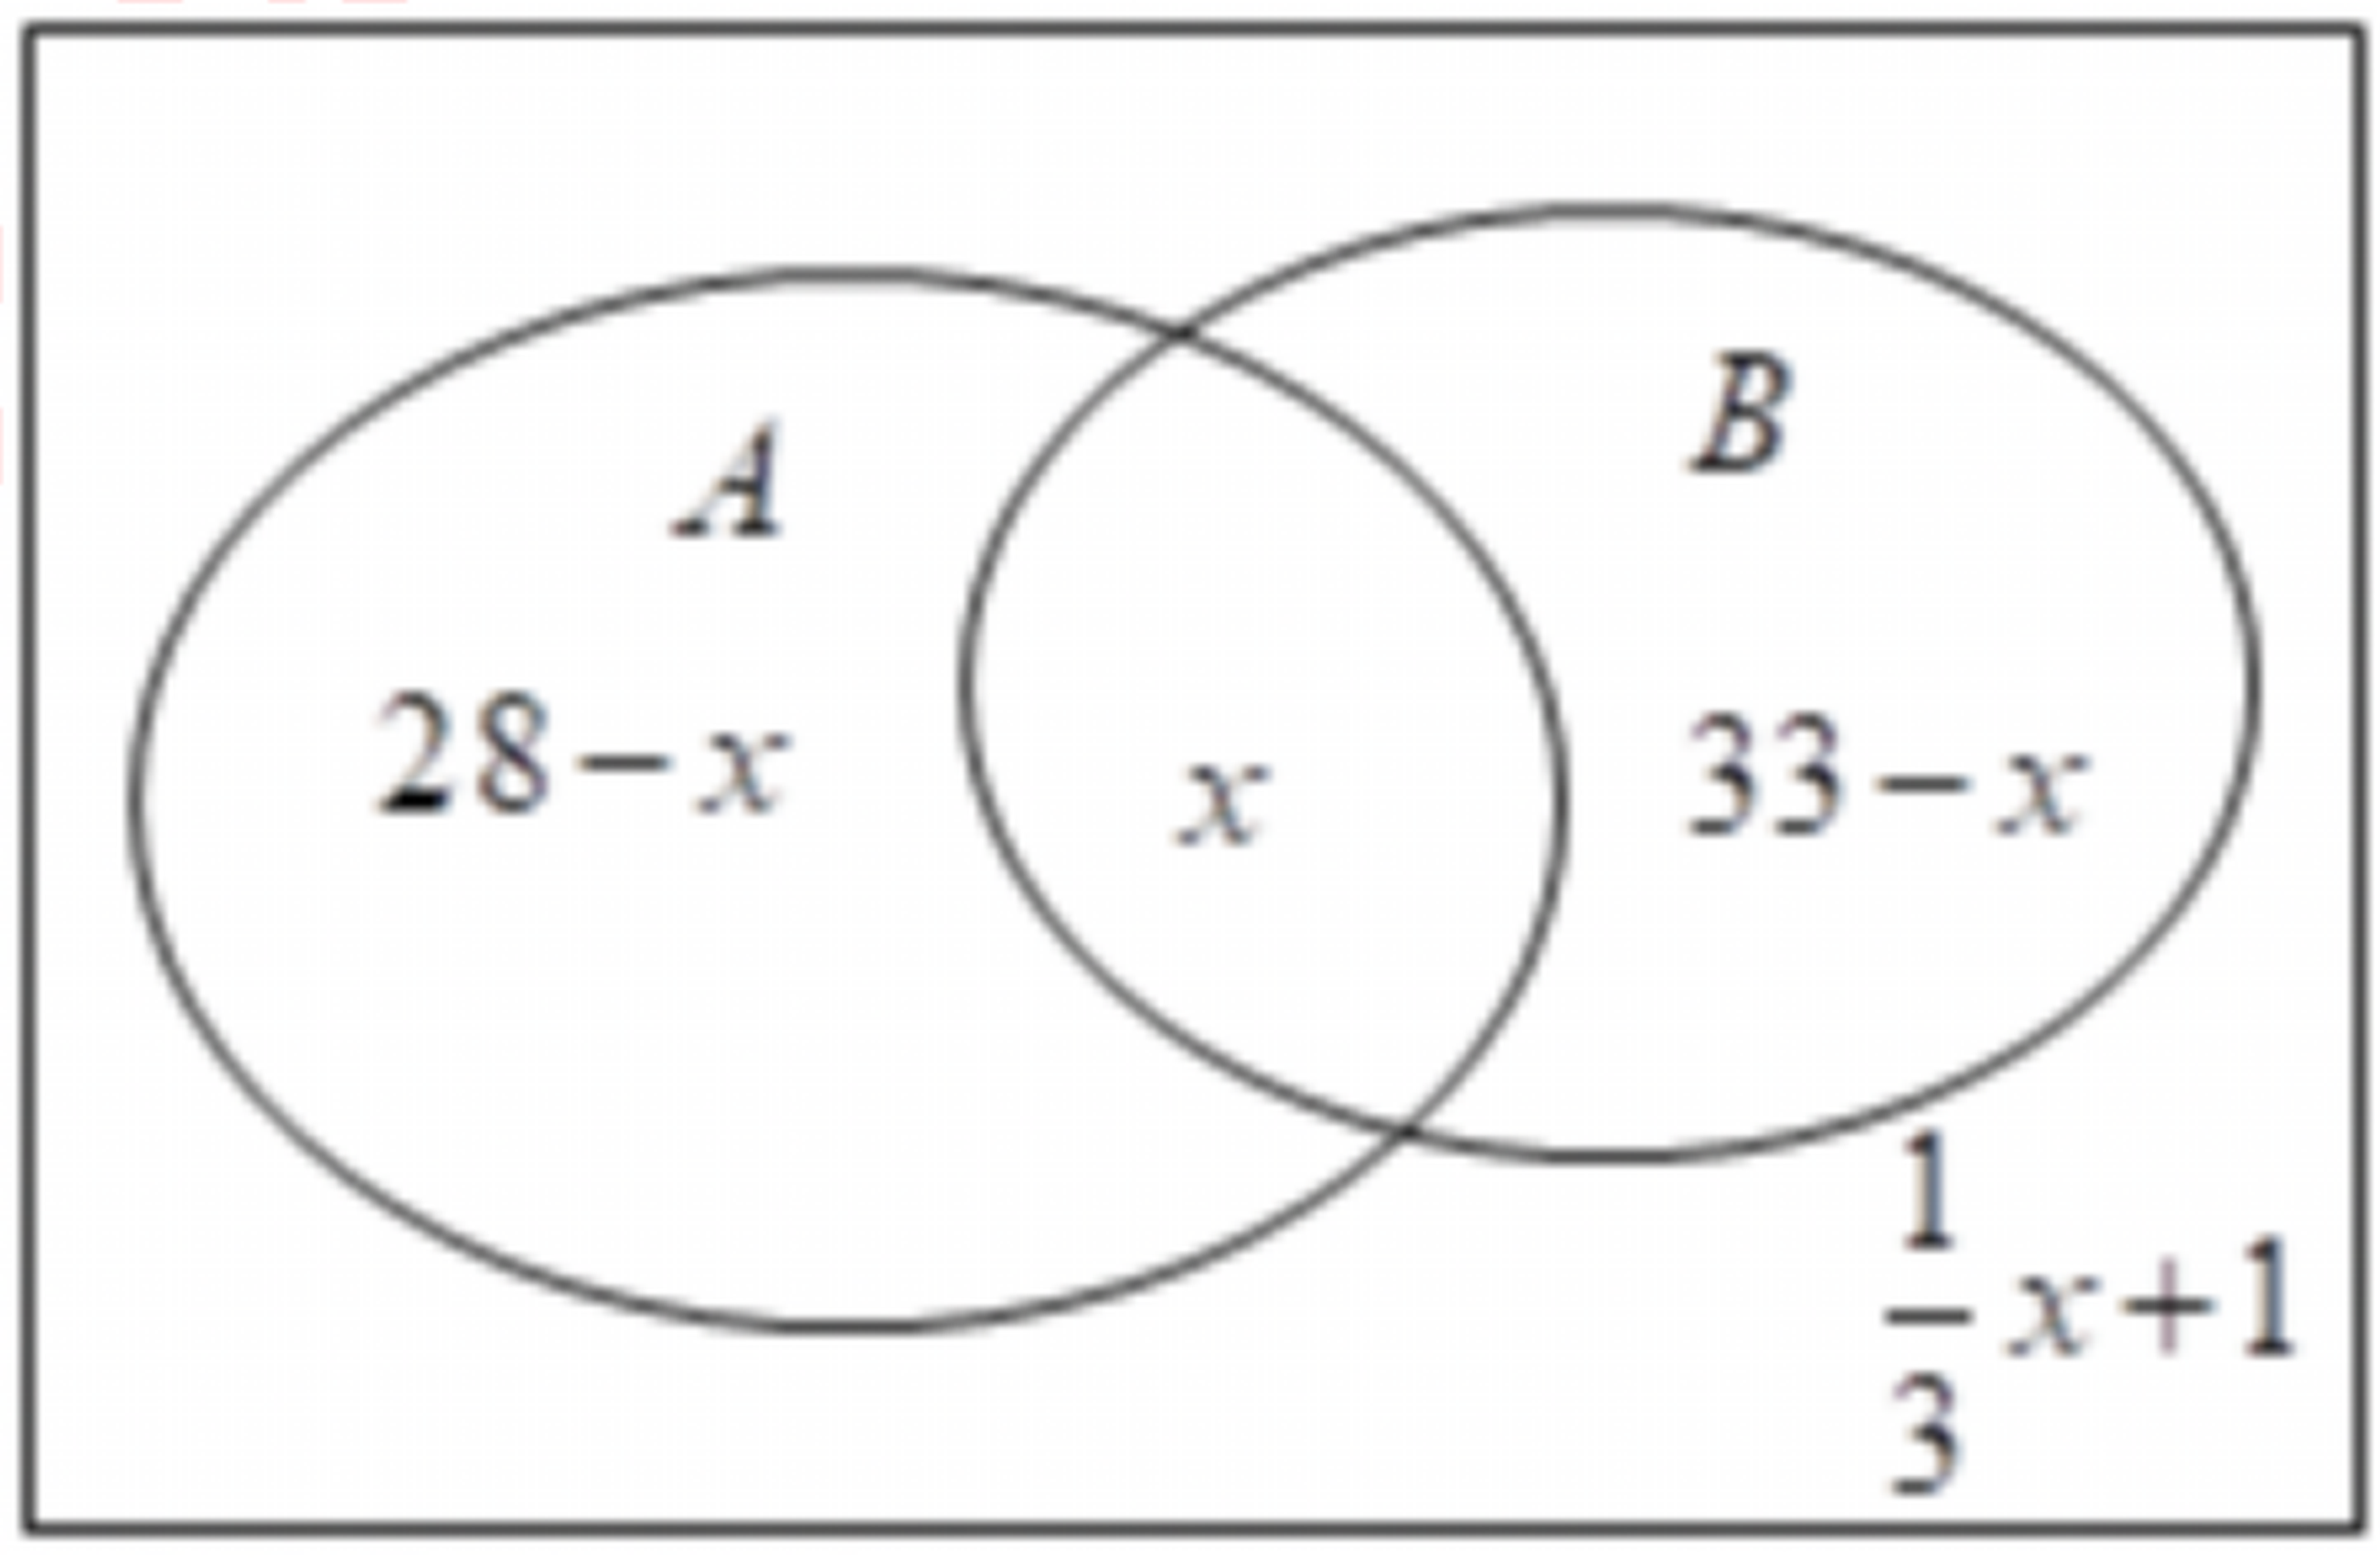
\includegraphics[width=0.42\textwidth]{figures/venn_AB_survey_50_x.png}
\end{center}
\step{则仅参加 $A$ 项的有 $(28-x)$ 人，仅参加 $B$ 项的有 $(33-x)$ 人，}
\step{$A$、$B$ 两项公益活动都不参加的有 $\left(\dfrac13x+1\right)$ 人，}
\step{由题意得 $x+(28-x)+(33-x)+\left(\dfrac13x+1\right)=50$，解得 $x=18$，}
\step{所以只参加 $A$ 项不参加 $B$ 项的有 $28-18=10$ 人.}
\solend
\fi

\item 设集合 $A=\{x\mid x^2-3x+2=0\}$，则满足 $A\cup B=\{0,1,2\}$ 的集合 $B$ 的个数是 \blankline[4.4em].

\ans{$4$}

\ifanswer
\solbegin
\step{$A=\{x\mid x^2-3x+2=0\}=\{x\mid x=1\text{ 或 }x=2\}=\{1,2\}$，}
\step{若 $A\cup B=\{0,1,2\}$，则 $0\in B$，}
\step{则 $B=\{0\},\{0,2\},\{1,0\},\{0,1,2\}$，共 $4$ 个.}
\solend
\fi

\item 已知全集 $U=\R$，集合 $A=\{x\mid x^2<4\}$，$B=\{y\mid y=x^2\}$，则图中阴影部分所表示的集合为 \blankline[4.4em].

\begin{center}
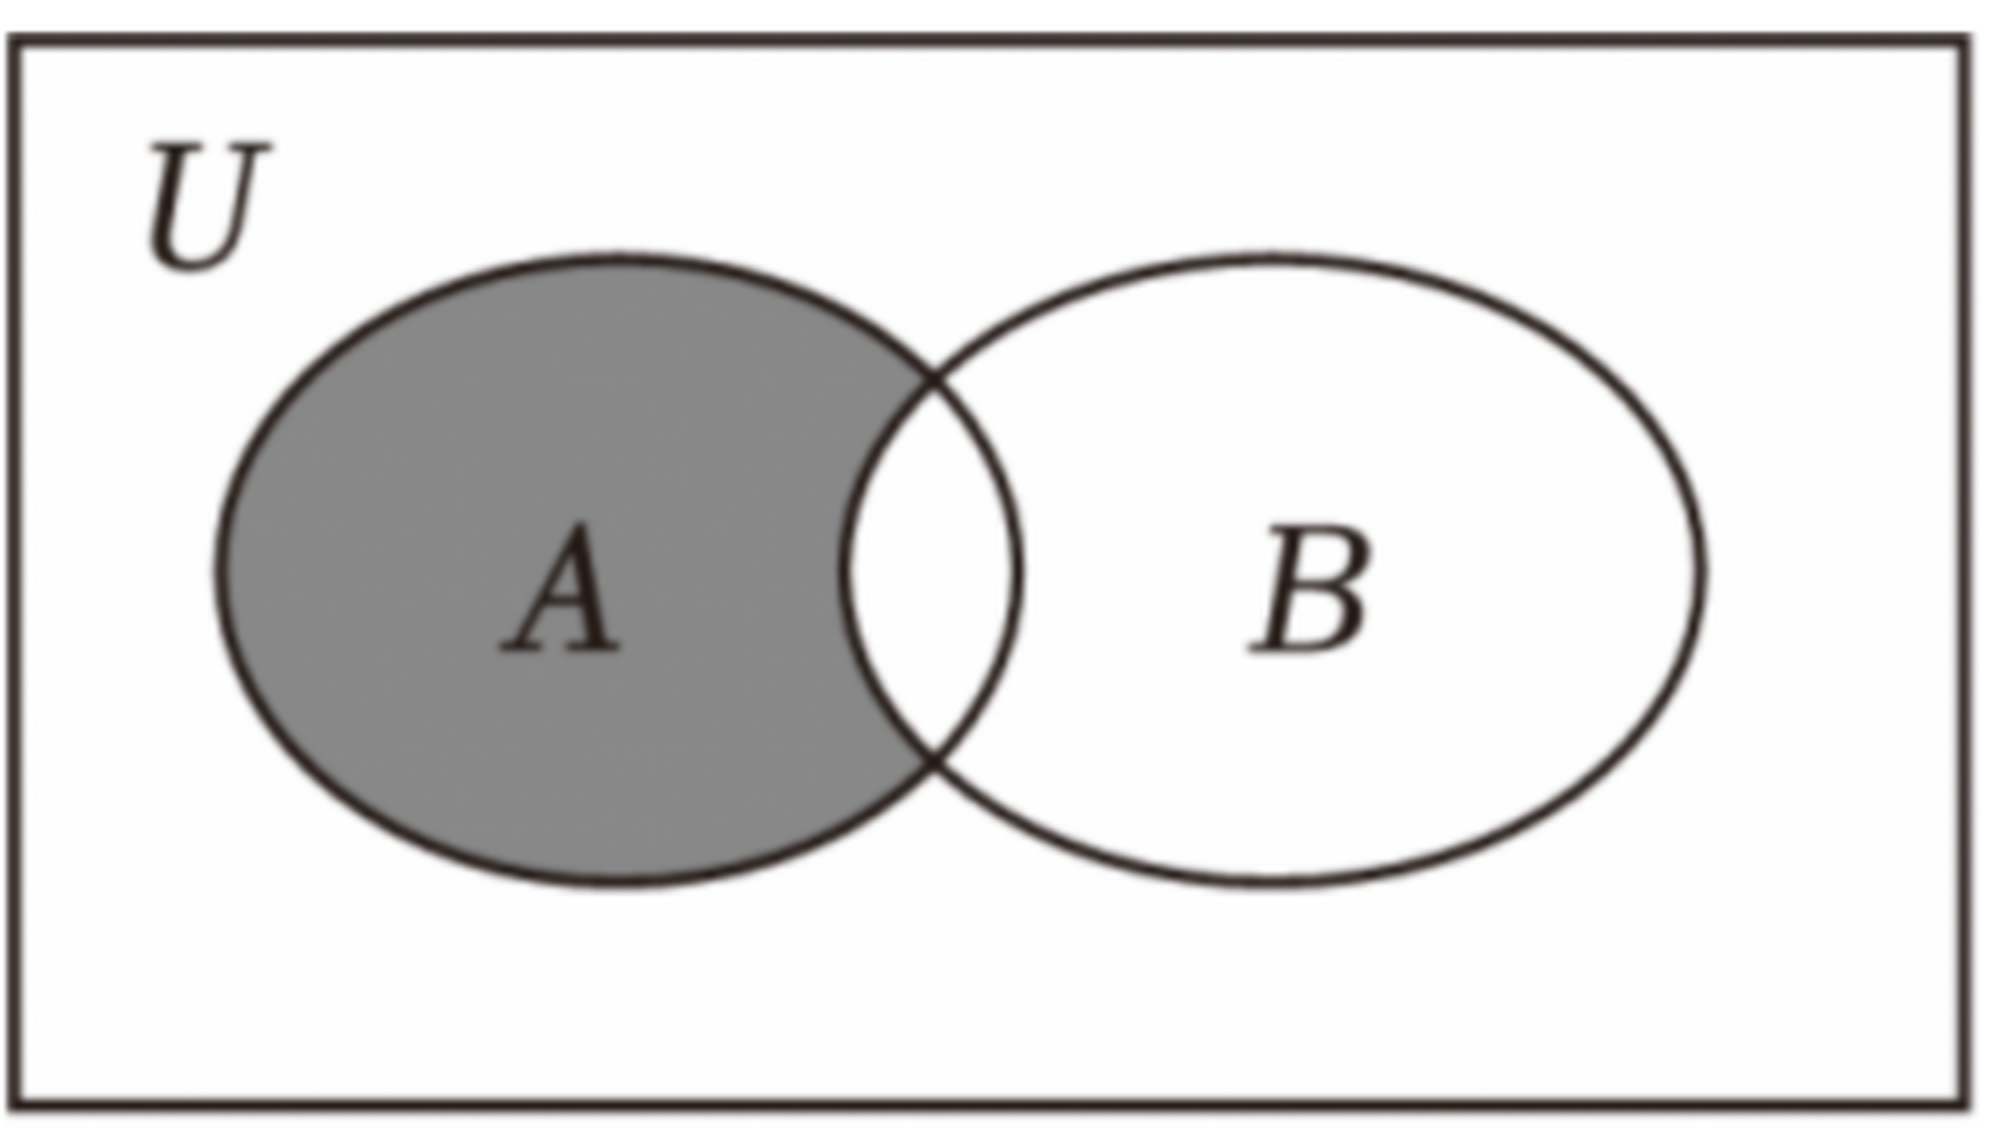
\includegraphics[width=0.34\textwidth]{figures/venn_A_shaded_U.png}
\end{center}

\ans{$A\cap\overline B=(-2,0)$}

\ifanswer
\solbegin
\step{集合 $A=\{x\mid x^2<4\}=(-2,2)$，$B=\{y\mid y=x^2\}=[0,+\infty)$，}
\step{图中阴影部分所表示的集合是 $A\cap\overline B=(-2,0)$.}
\solend
\fi

\item 如图所示，$M$、$P$、$S$ 是 $V$ 的三个子集，则阴影部分所表示的集合是 \blankline[5.4em].

\begin{center}
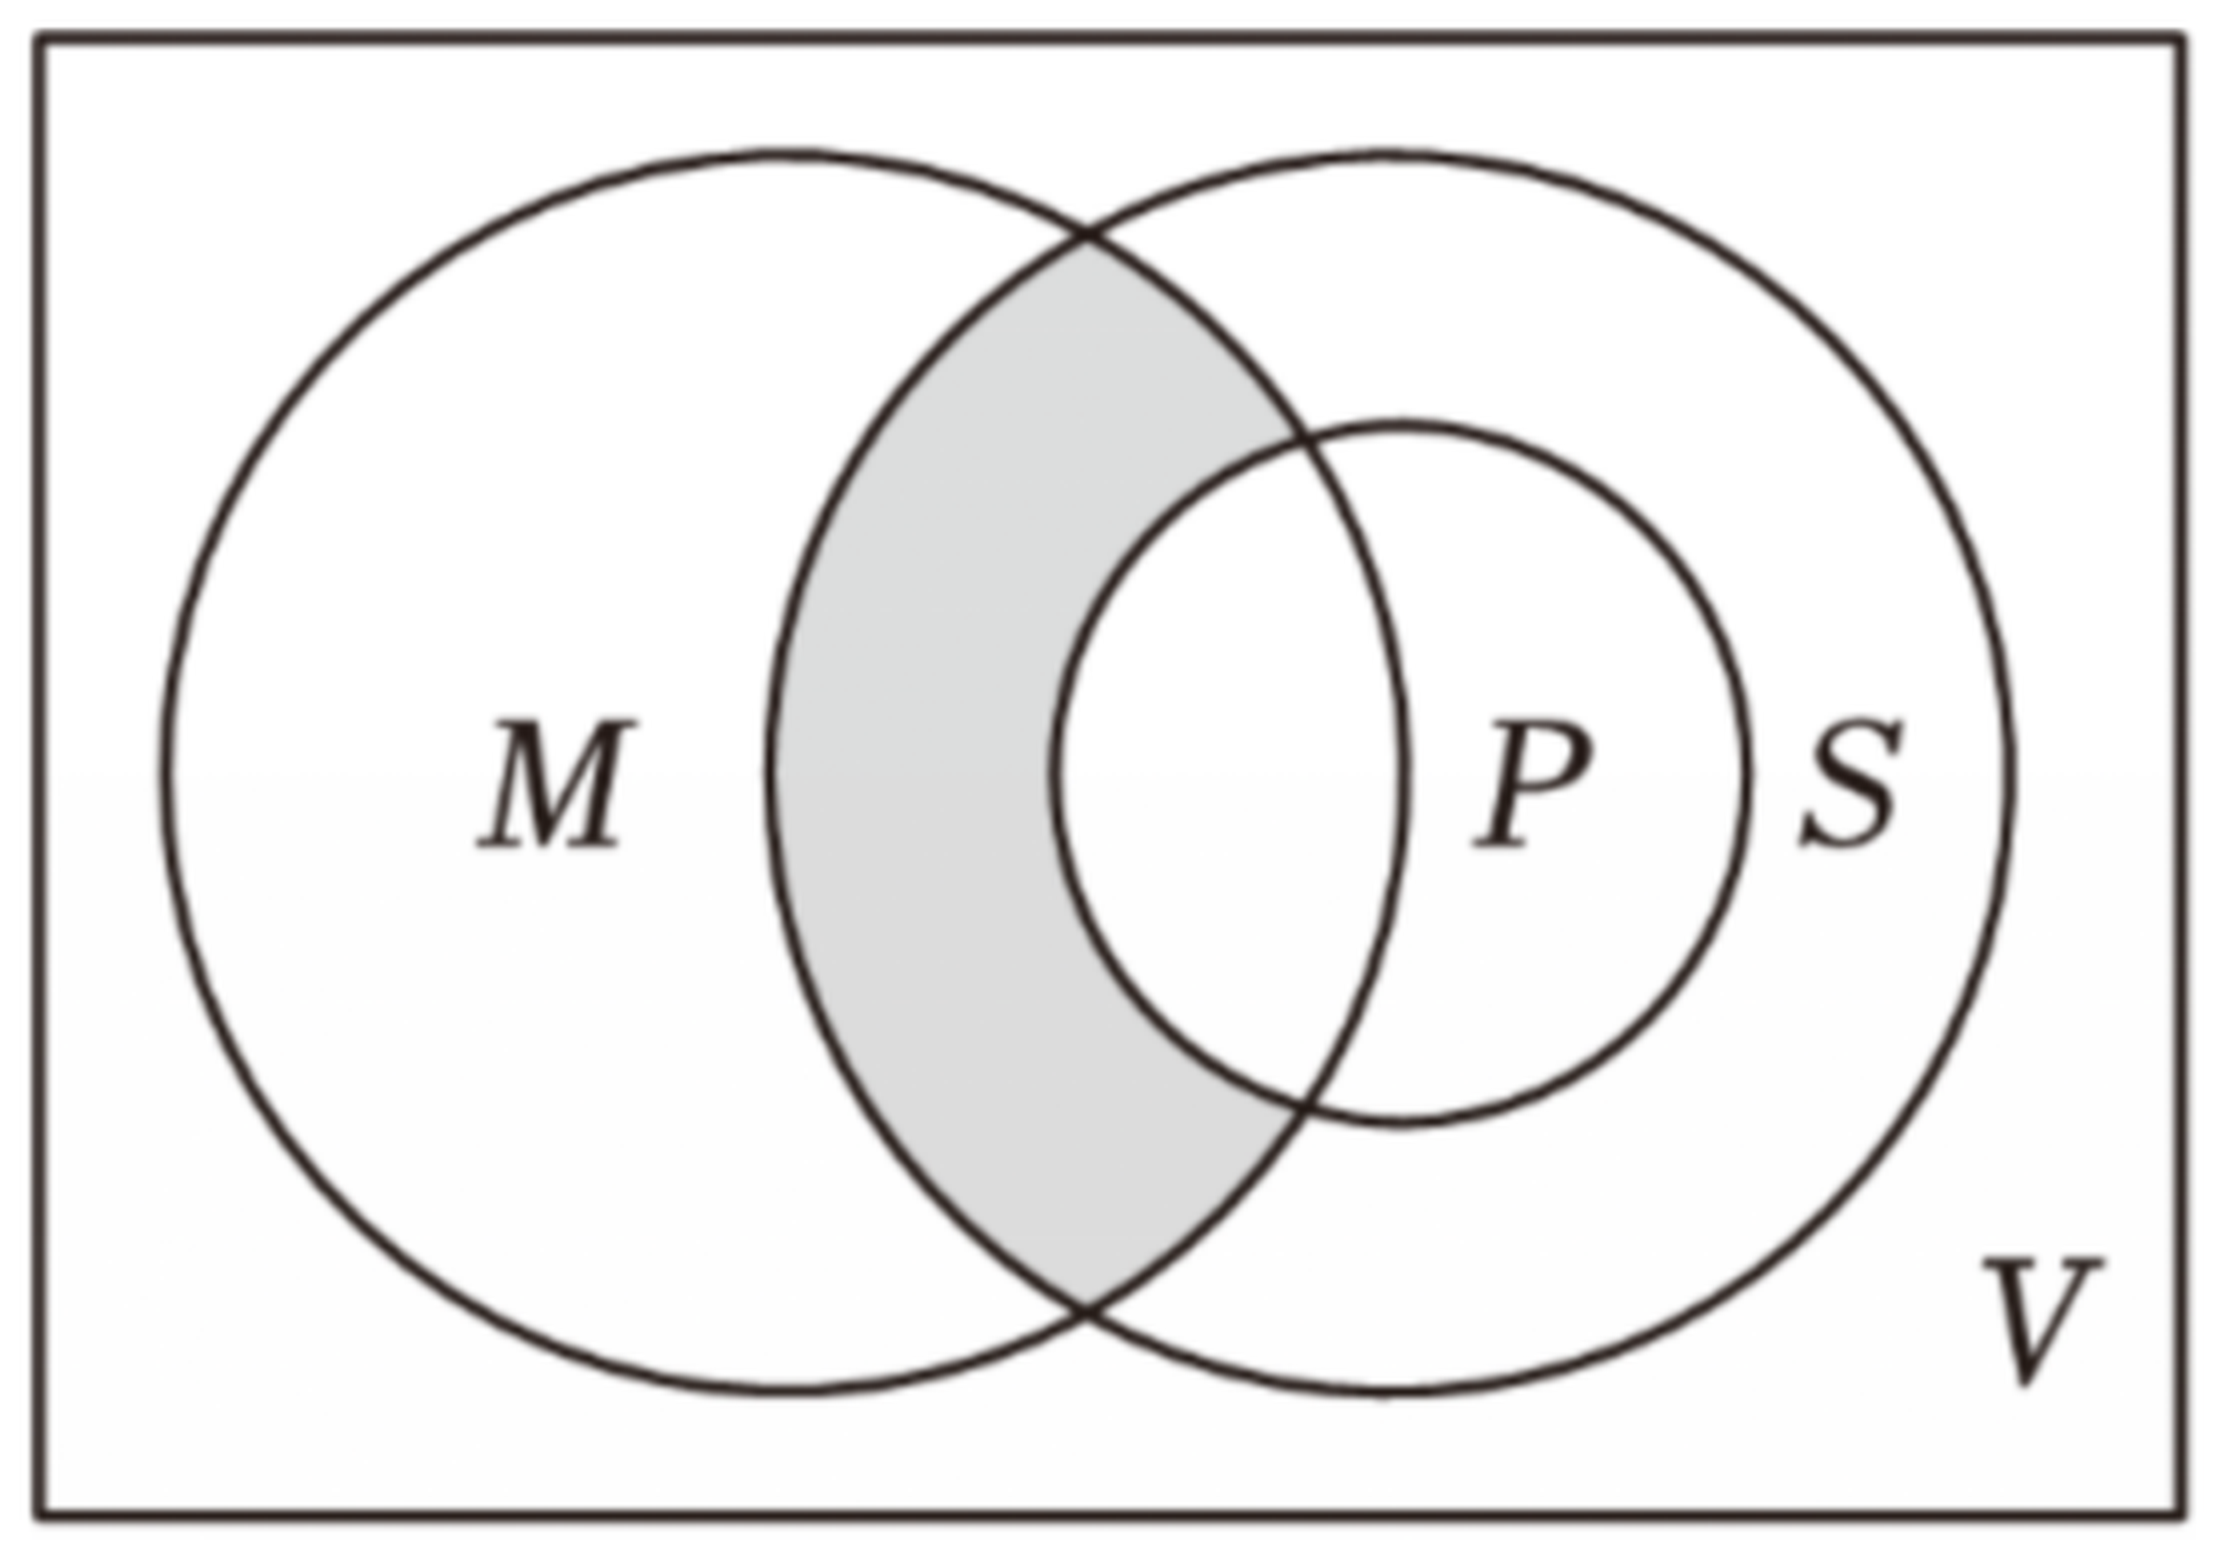
\includegraphics[width=0.38\textwidth]{figures/venn_MPS_V.png}
\end{center}

\ans{$(M\cap S)\cap(\complement_V P)$}

\item 下面六个关系式：① $\varnothing\subseteq\{a\}$；② $a\subseteq\{a\}$；③ $\{a\}\subseteq\{a\}$；④ $\{a\}\in\{a,b\}$；⑤ $a\in\{a,b,c\}$；⑥ $\varnothing\in\{a,b\}$；其中正确的是 \blankline[3.4em].

\ans{①③⑤}

\item 已知集合 $A=\{x\mid -1\le x\le a\}\ne\varnothing$，若 $\{y\mid y=x+1,x\in A\}=\{y\mid y=x^2,x\in A\}$，则实数 $a$ 值为 \blankline[4.4em].

\ans{$0$ 或 $\dfrac{1+\sqrt5}{2}$}

\ifanswer
\solbegin
\step{因为 $A=\{x\mid -1\le x\le a\}\ne\varnothing$，}
\step{所以 $\{y\mid y=x+1,x\in A\}=\{y\mid 0\le y\le a+1\}$，}
\step{$-1\le a\le1$ 时，$\{y\mid y=x^2,x\in A\}=\{y\mid 0\le y\le1\}$，}
\step{$a>1$ 时，$\{y\mid y=x^2,x\in A\}=\{y\mid 0\le y\le a^2\}$，}
\step{① $-1\le a\le1$ 时，$\{y\mid 0\le y\le a+1\}=\{y\mid 0\le y\le1\}$，则 $a+1=1$，解得 $a=0$；}
\step{② $a>1$ 时，$\{y\mid 0\le y\le a+1\}=\{y\mid 0\le y\le a^2\}$，则 $a^2=a+1$，解得 $a=\dfrac{1+\sqrt5}{2}$；}
\step{所以 $a=0$ 或 $\dfrac{1+\sqrt5}{2}$.}
\solend
\fi

\item 设集合 $A=\{(x,y)\mid x+y=22,x>0,y>0,x,y\text{ 均为质数}\}$ 的子集的个数为 \blankline[4.4em].

\ans{$32$}

\ifanswer
\solbegin
\step{集合 $A=\{(x,y)\mid x+y=22,x>0,y>0,x,y\text{ 均为质数}\}$}
\step{$=\{(3,19),(19,3),(5,17),(17,5),(11,11)\}$，则 $A$ 的子集的个数为 $2^5=32$.}
\solend
\fi

% 注：原卷本题题干印作「已知一个有四个数字元素的集合 $S$」；「数字元素」疑为「元素」之衍，
%     但原卷字形确为「数字」二字（已 3× 放大核对过），本稿照录，不代为改写。
\item 已知一个有四个数字元素的集合 $S$，$S$ 的所有子集的元素和（空集的元素和认为是 $0$）的总和为 $16192$，则 $S$ 的元素之和等于 \blankline[4.4em].

\ans{$2024$}

\ifanswer
\solbegin
\step{设 $S=\{a_1,a_2,a_3,a_4\}$，$S$ 的每个元素在所有子集中均出现 $2^3$ 次，}
\step{故 $(a_1+a_2+a_3+a_4)\cdot 2^3=16192$，所以 $a_1+a_2+a_3+a_4=2024$，}
\step{故 $S$ 的元素之和等于 $2024$.}
\solend
\fi

\item 设 $A$ 是非空数集，若对任意 $x$、$y\in A$，都有 $x+y\in A$、$xy\in A$，则称 $A$ 具有性质 $P$，给出以下命题：

①若 $A$ 具有性质 $P$，则 $A$ 可以是有限集；

②若 $A$ 具有性质 $P$，且 $A\ne\R$，则 $\overline A$ 具有性质 $P$；

③若 $A_1$、$A_2$ 具有性质 $P$，且 $A_1\cap A_2\ne\varnothing$，则 $A_1\cap A_2$ 具有性质 $P$；

④若 $A_1$、$A_2$ 具有性质 $P$，则 $A_1\cap A_2$ 具有性质 $P$.

其中所有真命题的序号是 \blankline[4.4em].

\ans{①③}

\ifanswer
\solbegin
\step{对于①，取集合 $A=\{0,1\}$ 具有性质 $P$，故 $A$ 可以是有限集，故①正确；}
\step{对于③，取 $x$、$y\in A_1\cap A_2$，则 $x\in A_1$，$x\in A_2$，$y\in A_1$，$y\in A_2$，}
\step{又 $A_1$、$A_2$ 具有性质 $P$，所以 $x+y\in A_1$，$xy\in A_1$，$x+y\in A_2$，$xy\in A_2$，}
\step{所以 $x+y\in A_1\cap A_2$，$xy\in A_1\cap A_2$，所以 $A_1\cap A_2$ 具有性质 $P$，故③正确；}
\step{对于④，取 $A_1=\{x\mid x=2k,k\in\Z\}$，$A_2=\{x\mid x=3k,k\in\Z\}$，$2\in A_1$，$3\in A_2$，}
\step{但 $2+3\notin A_1\cup A_2$，故④错误；}
\step{对于②，若 $A$ 具有性质 $P$，且 $A\ne\R$，假设 $\overline A$ 也具有性质 $P$，}
\step{设 $0\in A$，在 $\overline A$ 中任取一个 $x$，$x\ne0$，此时可证得 $-x\in A$，}
\step{否则若 $-x\in\overline A$，由于 $\overline A$ 也具有性质 $P$，则 $x+(-x)=0\in\overline A$，}
\step{与 $0\in A$ 矛盾，故 $-x\in A$，}
\step{由于 $A$ 具有性质 $P$，$\overline A$ 也具有性质 $P$，所以 $(-x)^2\in A$，$x^2\in\overline A$，}
\step{而 $(-x)^2=x^2$，这与 $A\cap\overline A=\varnothing$ 矛盾，}
\step{故当 $0\in A$ 且 $A$ 具有性质 $P$ 时，则 $\overline A$ 不具有性质 $P$，}
\step{同理当 $0\in\overline A$ 时，也可以类似推出矛盾，故②错误.}
\step{故正确的是①③.}
\solend
\fi

\item 已知 $S=\{1,2,3,4,5\}$，$A=\{1,2,5\}$，$T=\{t_1,t_2\}\subseteq S$，记 $A_1=\{x\mid x=a+t_1,a\in A,t_1\in T\}$，$A_2=\{x\mid x=b+t_2,b\in A,t_2\in T\}$，若 $A_1\cap A_2=\varnothing$，则集合 $T$ 为 \blankline[5.4em].

\ans{$T=\{1,3\}$ 或 $T=\{2,4\}$ 或 $T=\{3,5\}$}

\ifanswer
\solbegin
\step{若 $A_1\cap A_2=\varnothing$，即 $a+t_1\ne b+t_2$，则 $t_1-t_2\ne a-b$，其中 $a$、$b\in A$，}
\step{否则 $t_1+a=t_2+b$，$A_1\cap A_2\ne\varnothing$，}
\step{又 $S=\{1,2,3,4,5\}$，$A=\{1,2,5\}$，$T=\{t_1,t_2\}\subseteq S$，}
\step{$2-1=1$，$5-2=3$，$5-1=4$，则 $t_1$、$t_2$ 相差 $2$，}
\step{所以 $T=\{1,3\}$ 或 $T=\{2,4\}$ 或 $T=\{3,5\}$.}
\solend
\fi

\end{enumerate}

\bigsec{二、解答题}

\begin{enumerate}
\setcounter{enumi}{13}

\item 设集合 $P=\{1,2,3,m\}$，$Q=\{3,m^2\}$，且 $\overline P\cap Q=\varnothing$，求实数 $m$ 的值组成的集合.

\ans{$\{-1,0,\pm\sqrt2\}$}

\ansspace[5]

\ifanswer
\solbegin
\step{因为 $\overline P\cap Q=\varnothing$，所以 $Q\subseteq P$，所以 $m^2=1$ 或 $m^2=2$ 或 $m^2=m$，}
\step{考虑互异性，得 $m=-1$ 或 $m=\pm\sqrt2$ 或 $m=0$，}
\step{所以实数 $m$ 的值组成的集合为 $\{-1,0,\pm\sqrt2\}$.}
\solend
\fi

\item 若集合 $A=(-\infty,2]$，$B=\{x\mid kx+1<0,k\in\R\}$，$A\cap B=\varnothing$，求实数 $k$ 的取值范围.

\ans{$\left[-\dfrac12,0\right]$}

\ansspace[5]

\ifanswer
\solbegin
\step{若 $B=\varnothing$，则 $k=0$，符合题意，}
\step{若 $B\ne\varnothing$，当 $k>0$ 时，$B=\left(-\infty,-\dfrac1k\right)$，$A\cap B\ne\varnothing$，不合题意；}
\step{当 $k<0$ 时，$B=\left(-\dfrac1k,+\infty\right)$，由 $A\cap B=\varnothing$ 得 $-\dfrac1k\ge2$，即 $-\dfrac12\le k<0$，}
\step{故 $k$ 的取值范围是 $\left[-\dfrac12,0\right]$.}
\solend
\fi

\item 已知集合 $A=\{-4,2a-1,a^2\}$，$B=\{a-5,1-a,9\}$，分别求适合下列条件的 $a$ 的值.

% 两个小问不许与题干分家：试卷版第 2 页页末原本正好把 (1) 留在页底、(2) 翻到次页，
% 与 2026-09-15 修的三类难看切页同源，故在这里也加 \keepwithprev 守卫（三版都生效）。
\keepwithprev
（1）$9\in(A\cap B)$；

\keepwithprev
（2）$\{9\}=A\cap B$.

\ans{（1）$a=5$ 或 $a=-3$；（2）$a=-3$}

\ansspace[5]

\ifanswer
\solbegin
\stepm{（1）}{$9\in(A\cap B)$，所以 $9\in A$，}
\step{当 $2a-1=9$ 时，$a=5$，当 $a^2=9$ 时，即 $a=\pm3$，}
% 注：原卷此句结论印作「所以 $a$ 的值为 $5\backslash-3$」——「\」应是顿号之误，
%     本稿照录原卷字形（见文件头「原卷存疑」②）；按文意即 $a=5$ 或 $a=-3$。
\step{当 $a=3$ 时，$a-5=1-a$ 舍去，所以 $a$ 的值为 $5\backslash-3$.}
\stepm{（2）}{结合（1）的结论：}
\step{当 $2a-1=9$ 即 $a=5$ 时，$1-a=-4$，$\{9\}\ne(A\cap B)$，}
\step{当 $a^2=9$ 时，即 $a=\pm3$，当 $a=3$ 时，$a-5=1-a$ 舍去，}
\step{所以 $a$ 的值为 $-3$.}
\solend
\fi

\item 已知集合 $M=\{a,ab,a-b\}$，$N=\{0,|a|,b\}$，且 $M=N$，求实数 $a$、$b$ 的值.

\ans{$a=b=-1$}

\ansspace[5]

\ifanswer
\solbegin
\step{由集合元素的互异性，得 $a\ne0$，且 $b\ne0$，所以 $a-b=0$，即 $a=b$，}
\step{所以 $ab=|a|$，又由 $|a|\ne b=a$，得 $a<0$，故 $a=b=-1$.}
\solend
\fi

\item 已知集合 $A=\{x\mid -2<x<7\}$，$B=\{x\mid m+1\le x\le 2m-1\}$.

\keepwithprev
（1）当 $m=4$ 时，求 $A\cap B$、$A\cup B$；

\keepwithprev
（2）若 $A\cap B=B$，求实数 $m$ 的取值范围.

\ans{（1）$A\cap B=[5,7)$，$A\cup B=(-2,7]$；（2）$(-\infty,4)$}

\ansspace[5]

\ifanswer
\solbegin
\stepm{（1）}{当 $m=4$ 时，得集合 $A=\{x\mid -2<x<7\}$，$B=\{x\mid 5\le x\le7\}$，}
\step{得 $A\cap B=[5,7)$，$A\cup B=(-2,7]$.}
\stepm{（2）}{由 $A\cap B=B$ 得 $B\subseteq A$，}
\step{①当 $B=\varnothing$ 时，得 $m+1>2m-1$，解得 $m<2$；}
\step{②当 $B\ne\varnothing$ 时，得 $\begin{cases}m+1>-2\\ 2m-1<7\\ m+1\le2m-1\end{cases}$，解得 $2\le m<4$；}
\step{综上，实数 $m$ 的取值范围是 $(-\infty,4)$.}
\solend
\fi

\item 若集合 $A=\{x\mid x^2+5x-6=0\}$，$B=\{x\mid x^2+2(m+1)x+m^2-3=0\}$.

\keepwithprev
（1）当 $m=0$ 时，求集合 $A\cup B$；

\keepwithprev
（2）若 $A\cap B=B$，求实数 $m$ 的取值范围.

\ans{（1）$A\cup B=\{1,-6,-3\}$；（2）$\{m\mid m\le-2\}$}

\ansspace[5]

\ifanswer
\solbegin
\stepm{（1）}{由题意得，集合 $A=\{x\mid x^2+5x-6=0\}=\{1,-6\}$，}
\step{当 $m=0$ 时，$B=\{x\mid x^2+2x-3=0\}=\{1,-3\}$，}
\step{所以 $A\cup B=\{1,-6,-3\}$；}
\stepm{（2）}{由（1）得集合 $A=\{1,-6\}$，$B=\{x\mid x^2+2(m+1)x+m^2-3=0\}$，}
\step{若 $A\cap B=B$ 得 $B\subseteq A$，所以 $B=\varnothing$ 或 $\{-6\}$ 或 $\{1\}$ 或 $\{1,-6\}$，}
\step{当 $B=\varnothing$ 时，$\Delta=4(m+1)^2-4(m^2-3)<0$，解得 $m<-2$，}
\step{当 $B=\{-6\}$ 时，则 $\begin{cases}\Delta=4(m+1)^2-4(m^2-3)=0\\ 36-12(m+1)+m^2-3=0\end{cases}$，无解，}
\step{当 $B=\{1\}$ 时，则 $\begin{cases}\Delta=4(m+1)^2-4(m^2-3)=0\\ 1+2(m+1)+m^2-3=0\end{cases}$，解得 $m=-2$，}
\step{当 $B=\{1,-6\}$ 时，则 $\begin{cases}\Delta=4(m+1)^2-4(m^2-3)>0\\ 1+(-6)=-2(m+1)\\ 1\times(-6)=m^2-3\end{cases}$，无解，}
\step{综上所述，实数 $m$ 的取值范围为 $\{m\mid m\le-2\}$.}
\solend
\fi

% 压轴题：其后已无内容，故作答区全用可丢弃胶水（\ansspace*），并在题目前先量一下版面。
\ansneed{8cm}
\item 对于点集 $A=\{(x,y)\mid x=m,y=-3x+2,m\in\N,m\ge1\}$，$B=\{(x,y)\mid x=n,y=a(x^2-x+1),n\in\N,n\ge1\}$，是否存在非零整数 $a$，使得 $A\cap B\ne\varnothing$？

\ans{$a=-1$}

\ansspace*[10]

\ifanswer
\solbegin
\step{当 $A\cap B\ne\varnothing$ 时，$-3x+2=a(x^2-x+1)$，}
\step{$ax^2+(3-a)x+a-2=0$ ①有正整数解，}
\step{所以 $\Delta=(3-a)^2-4a(a-2)=-3a^2+2a+9$ 是平方数，}
\step{所以 $3a^2-2a-9\le0$，$\dfrac{1-2\sqrt7}{3}\le a\le\dfrac{1+2\sqrt7}{3}$，$a\ne0$，$a\in\Z$，}
\step{所以 $a=\pm1$ 或 $a=2$，}
\step{$a=-1$ 时 $\Delta=4$，这时①变为 $-x^2+4x-3=0$，解得 $x_1=1$，$x_2=3$，}
\step{$A\cap B=\{(1,-1),(3,-7)\}$.}
\step{$a=1$ 时 $\Delta=8$，不是平方数.}
\step{$a=2$ 时 $\Delta=1$，这时①变为 $2x^2+x=0$，没有正整数解.}
\step{所以 $a=-1$.}
\solend
\fi

\end{enumerate}

\end{document}
"
% 紧凑版：xelatex "\def\iscompact{1}% 高一19_延安中学_周末作业2.tex —— 高一上数学「2026-2027 年延安中学高一上周末作业 2」（试卷版/答案版）
% 试卷版：xelatex 高一19_延安中学_周末作业2.tex
% 答案版：xelatex "\def\isanswer{1}% 高一19_延安中学_周末作业2.tex —— 高一上数学「2026-2027 年延安中学高一上周末作业 2」（试卷版/答案版）
% 试卷版：xelatex 高一19_延安中学_周末作业2.tex
% 答案版：xelatex "\def\isanswer{1}% 高一19_延安中学_周末作业2.tex —— 高一上数学「2026-2027 年延安中学高一上周末作业 2」（试卷版/答案版）
% 试卷版：xelatex 高一19_延安中学_周末作业2.tex
% 答案版：xelatex "\def\isanswer{1}\input{高一19_延安中学_周末作业2.tex}"
% 紧凑版：xelatex "\def\iscompact{1}\input{高一19_延安中学_周末作业2.tex}"
%
% 原始材料是微信公众号图文（公众号「魔都数学加油站」，作者署名「破晓」，
% 原文链接 https://mp.weixin.qq.com/s/tHqWSV1StO5SHSXXQ4jeUA），正文为 6 张 PNG 页；
% 原文本身就是一份**讲评版**——题目下方直接印出【答案】或【解析】。本稿把答案与解析
% 移到答案版，试卷版即一张干净的空卷；试题文字、答案与解析均照原卷录入。
%
% 与原卷的排版差异（均已在 README「说明」中交代）：
%   ① 原文自**第 3 题**起（第 1、2 题未在该文发布），源码里以 \setcounter{enumi}{2} 起编；
%      全卷只有「一、填空题」「二、解答题」两节，无选择题；
%   ② 原卷本就印有两个分节标题（已在原图上逐页放大核对过），本稿照原卷分节，只把标题改排
%      成全稿统一的「大节标题」样式；
%   ③ 原卷的实数集、整数集、自然数集符号作正体 $R$、$Z$、$N$（第 15 题作粗体 $\mathbf{R}$，
%      第 20 题有 $N$ 与斜体 $Z$），本稿按全稿惯例统一写作 $\R$、$\Z$、$\N$；
%   ④ 第 4 题的韦恩图在原卷里印在【解析】右侧（题干并无「如图」二字），故本稿把该图放进
%      答案版的解析块内（`figures/venn_AB_survey_50_x.png`）；第 6、7 题的韦恩图是**题干图**
%      （题干作「图中阴影部分所表示的集合」），两版都排（`figures/venn_A_shaded_U.png`、
%      `figures/venn_MPS_V.png`）。三张图都取自原卷截图、4× LANCZOS 放大，不用 TikZ 手绘；
%   ⑤ 本卷也是「讲评版」，解析按全稿统一的 \solbegin/\step 分步重排（原卷为连续段落），
%      分步不改一字，只断句、断行；
%   ⑥ 标题前缀照**原卷**作「2026--2027 年…」（原卷标题即作「2026-2027年延安中学高一上周末
%      作业 2」）。同校的 高一06 作「学年度」——那是 高一02—高一09 那一批入库时统一改的；
%      后续入库的卷（高一10—高一17 与本卷）一律照原卷保留「年」，未强改，故同校两卷前缀不同。
%
% 原卷存疑两处（已逐处放大到能看清字形后核对，本稿照录并加注，见各题下的 `%` 注）：
%   （另有第三处「第 12 题【解析】末句」原先记作存疑，2026-09-26 第二轮核对放大后发现
%     原卷印的是「$0\in\overline A$」——A 上确有横杠，是本稿当初漏抄了 $\overline{}$；
%     已按原卷补回，故该条从存疑清单里删去，不计为原卷问题。）
%   ① 第 11 题题干印作「已知一个有四个数字元素的集合 $S$」，「数字元素」疑为「元素」之衍；
%   ② 第 16 题 (1) 结论印作「$a$ 的值为 $5\backslash-3$」，其中的「\」应是顿号之误
%      （由 (2) 的结论「$a$ 的值为 $-3$」可反推，(1) 的答案是 $5$ 或 $-3$）；

% 本篇在公众号「魔都数学加油站」连载里的编号是「27学年高一19」，本地编号与之对齐（高一19）；
% 对应关系见 README「与公众号连载号的对照表」。
\documentclass[a4paper,11pt]{article}
\usepackage{common}

\begin{document}

\examtitlest{2026--2027 年延安中学高一上周末作业 2}{集合与常用逻辑用语}

\bigsec{一、填空题}

\begin{enumerate}
% 原卷填空题从第 3 题起（1、2 未在该文中发布），须与解答题的 \setcounter{enumi}{13} 对齐
\setcounter{enumi}{2}
\item 已知全集 $U=\{1,2,3,4,5\}$，$M=\{1,2\}$，$P=\{1,3,5\}$，则 $M\cap\overline P=$ \blankline[4.4em].

\ans{$\{2\}$}

\item 某公司共有 $50$ 人，此次组织参加社会公益活动，其中参加 $A$ 项公益活动的有 $28$ 人，参加 $B$ 项公益活动的有 $33$ 人，且 $A$、$B$ 两项公益活动都不参加的人数比都参加的人数的三分之一多 $1$ 人，则只参加 $A$ 项不参加 $B$ 项的人数是 \blankline[4.4em].

\ans{$10$}

\ifanswer
\solbegin
\step{如图所示，设 $A$、$B$ 两项公益活动都参加的有 $x$ 人，}
\begin{center}
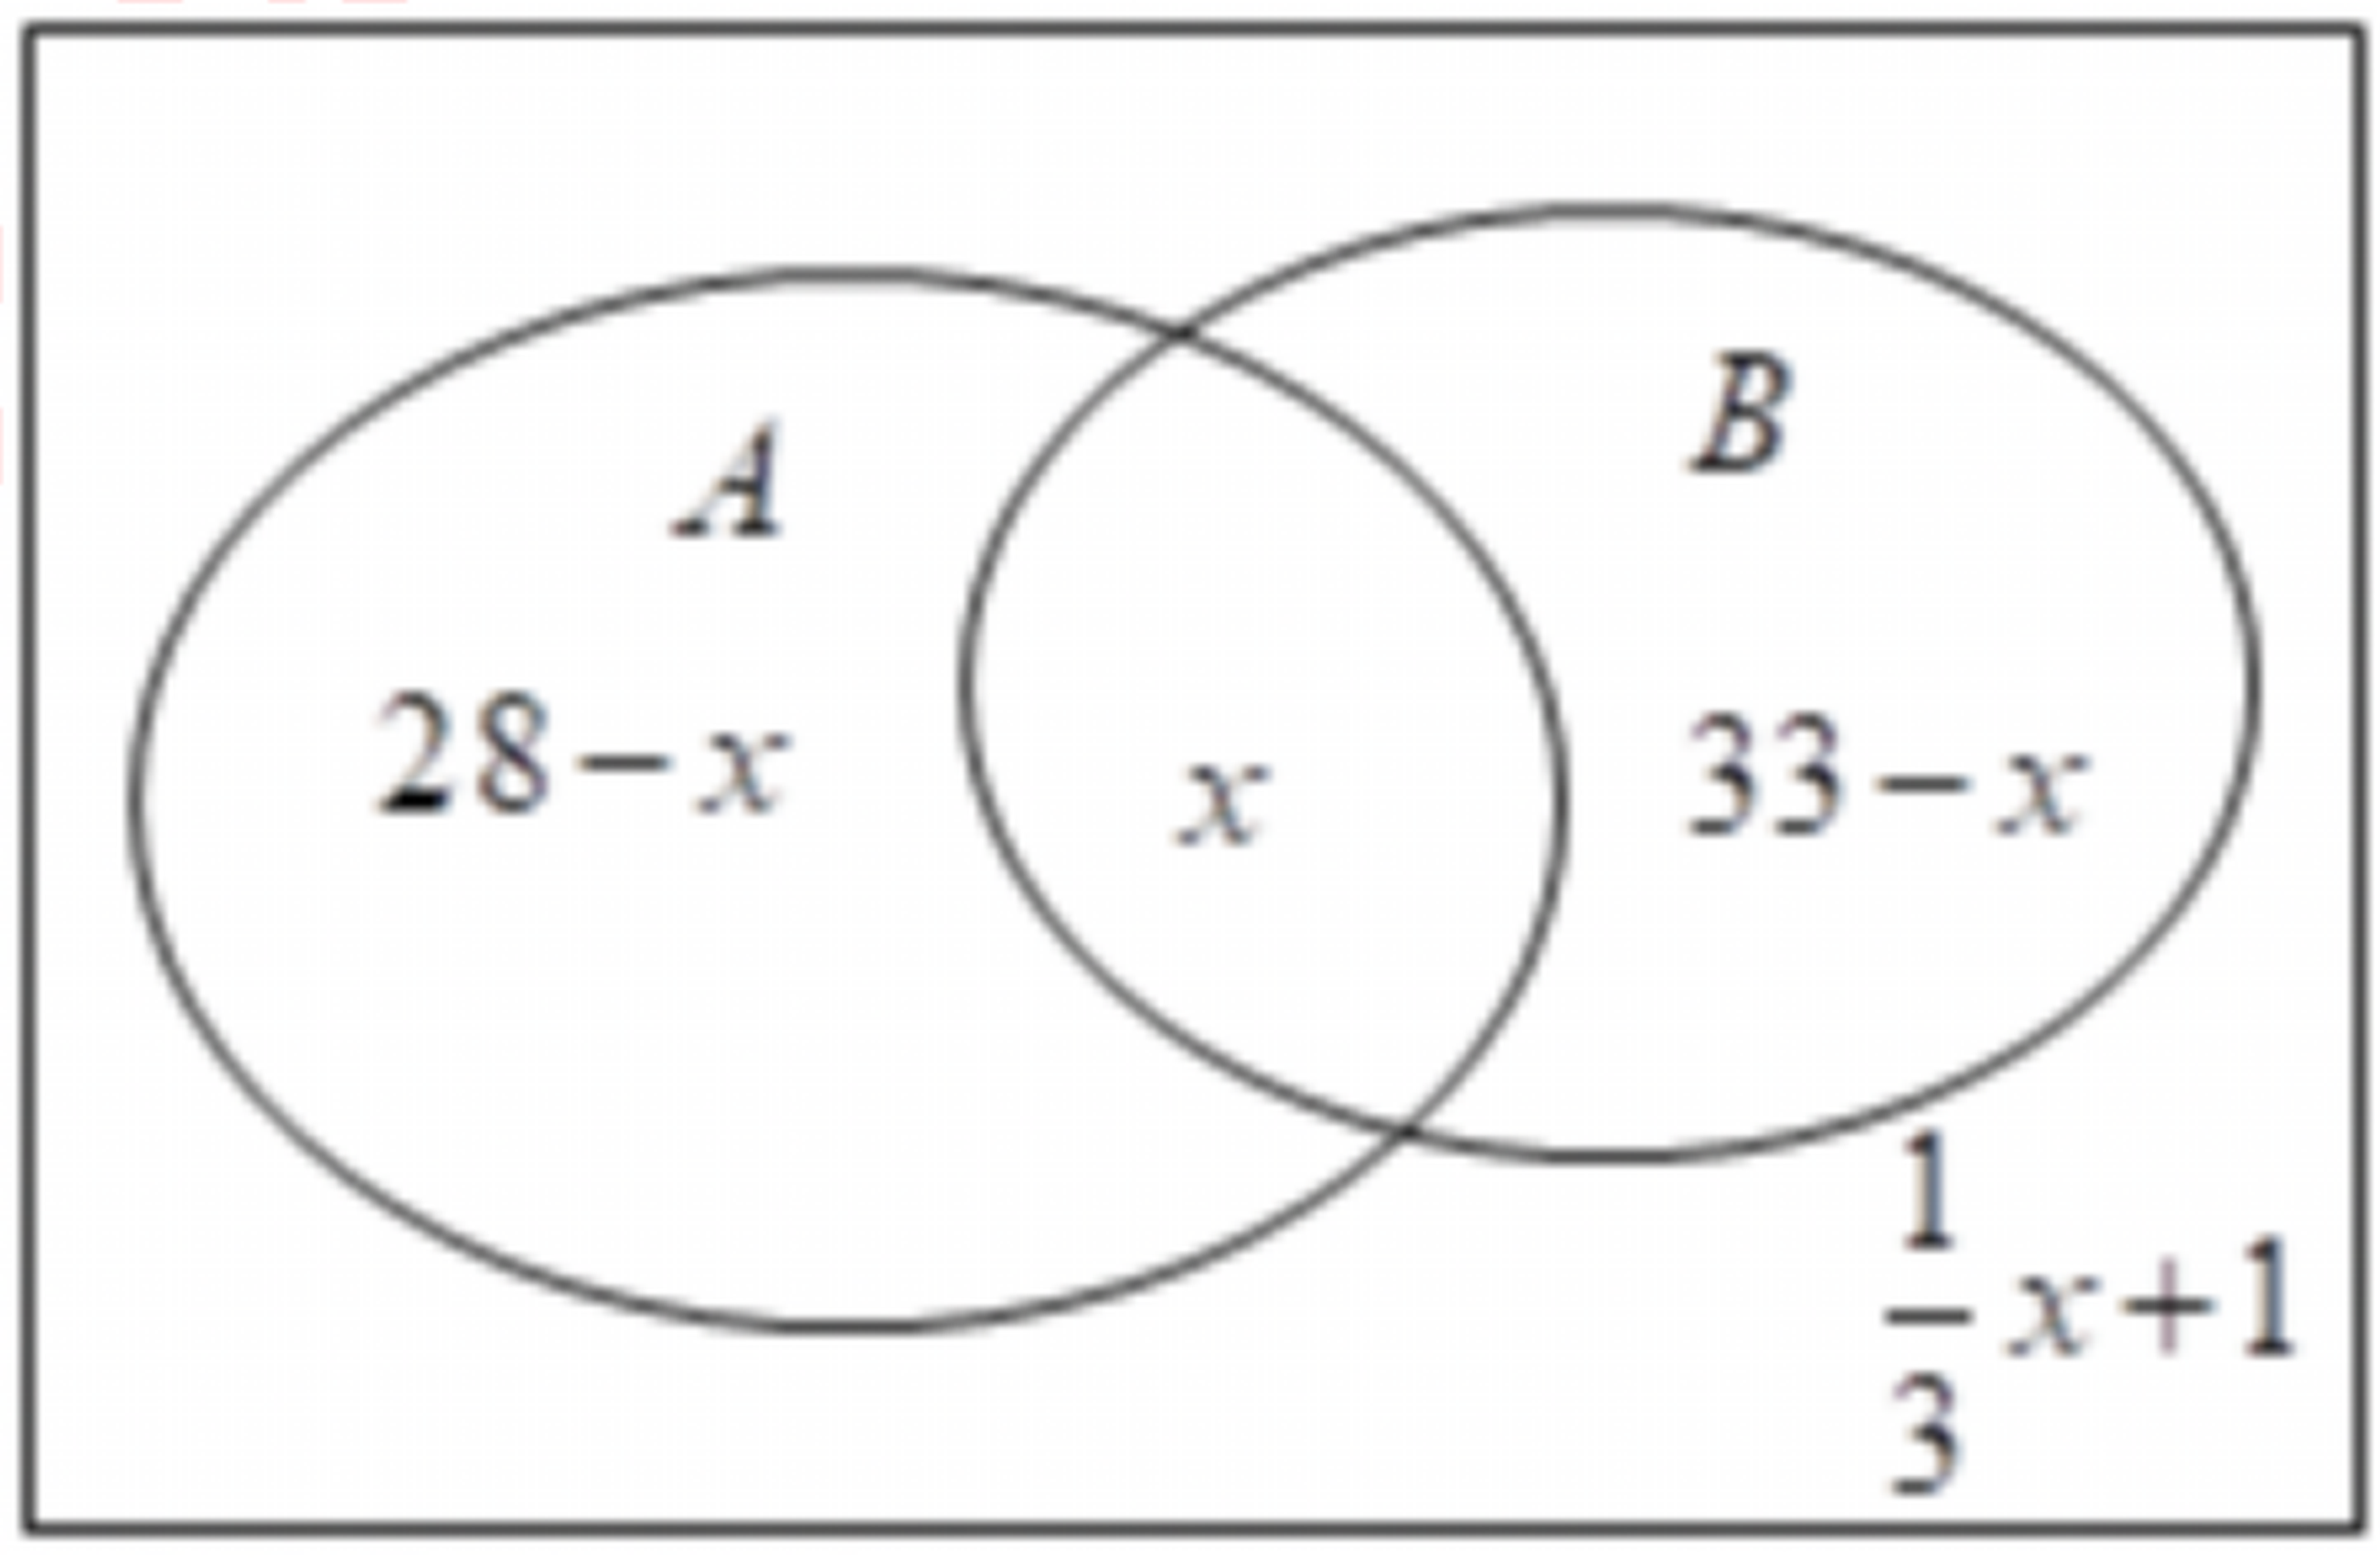
\includegraphics[width=0.42\textwidth]{figures/venn_AB_survey_50_x.png}
\end{center}
\step{则仅参加 $A$ 项的有 $(28-x)$ 人，仅参加 $B$ 项的有 $(33-x)$ 人，}
\step{$A$、$B$ 两项公益活动都不参加的有 $\left(\dfrac13x+1\right)$ 人，}
\step{由题意得 $x+(28-x)+(33-x)+\left(\dfrac13x+1\right)=50$，解得 $x=18$，}
\step{所以只参加 $A$ 项不参加 $B$ 项的有 $28-18=10$ 人.}
\solend
\fi

\item 设集合 $A=\{x\mid x^2-3x+2=0\}$，则满足 $A\cup B=\{0,1,2\}$ 的集合 $B$ 的个数是 \blankline[4.4em].

\ans{$4$}

\ifanswer
\solbegin
\step{$A=\{x\mid x^2-3x+2=0\}=\{x\mid x=1\text{ 或 }x=2\}=\{1,2\}$，}
\step{若 $A\cup B=\{0,1,2\}$，则 $0\in B$，}
\step{则 $B=\{0\},\{0,2\},\{1,0\},\{0,1,2\}$，共 $4$ 个.}
\solend
\fi

\item 已知全集 $U=\R$，集合 $A=\{x\mid x^2<4\}$，$B=\{y\mid y=x^2\}$，则图中阴影部分所表示的集合为 \blankline[4.4em].

\begin{center}
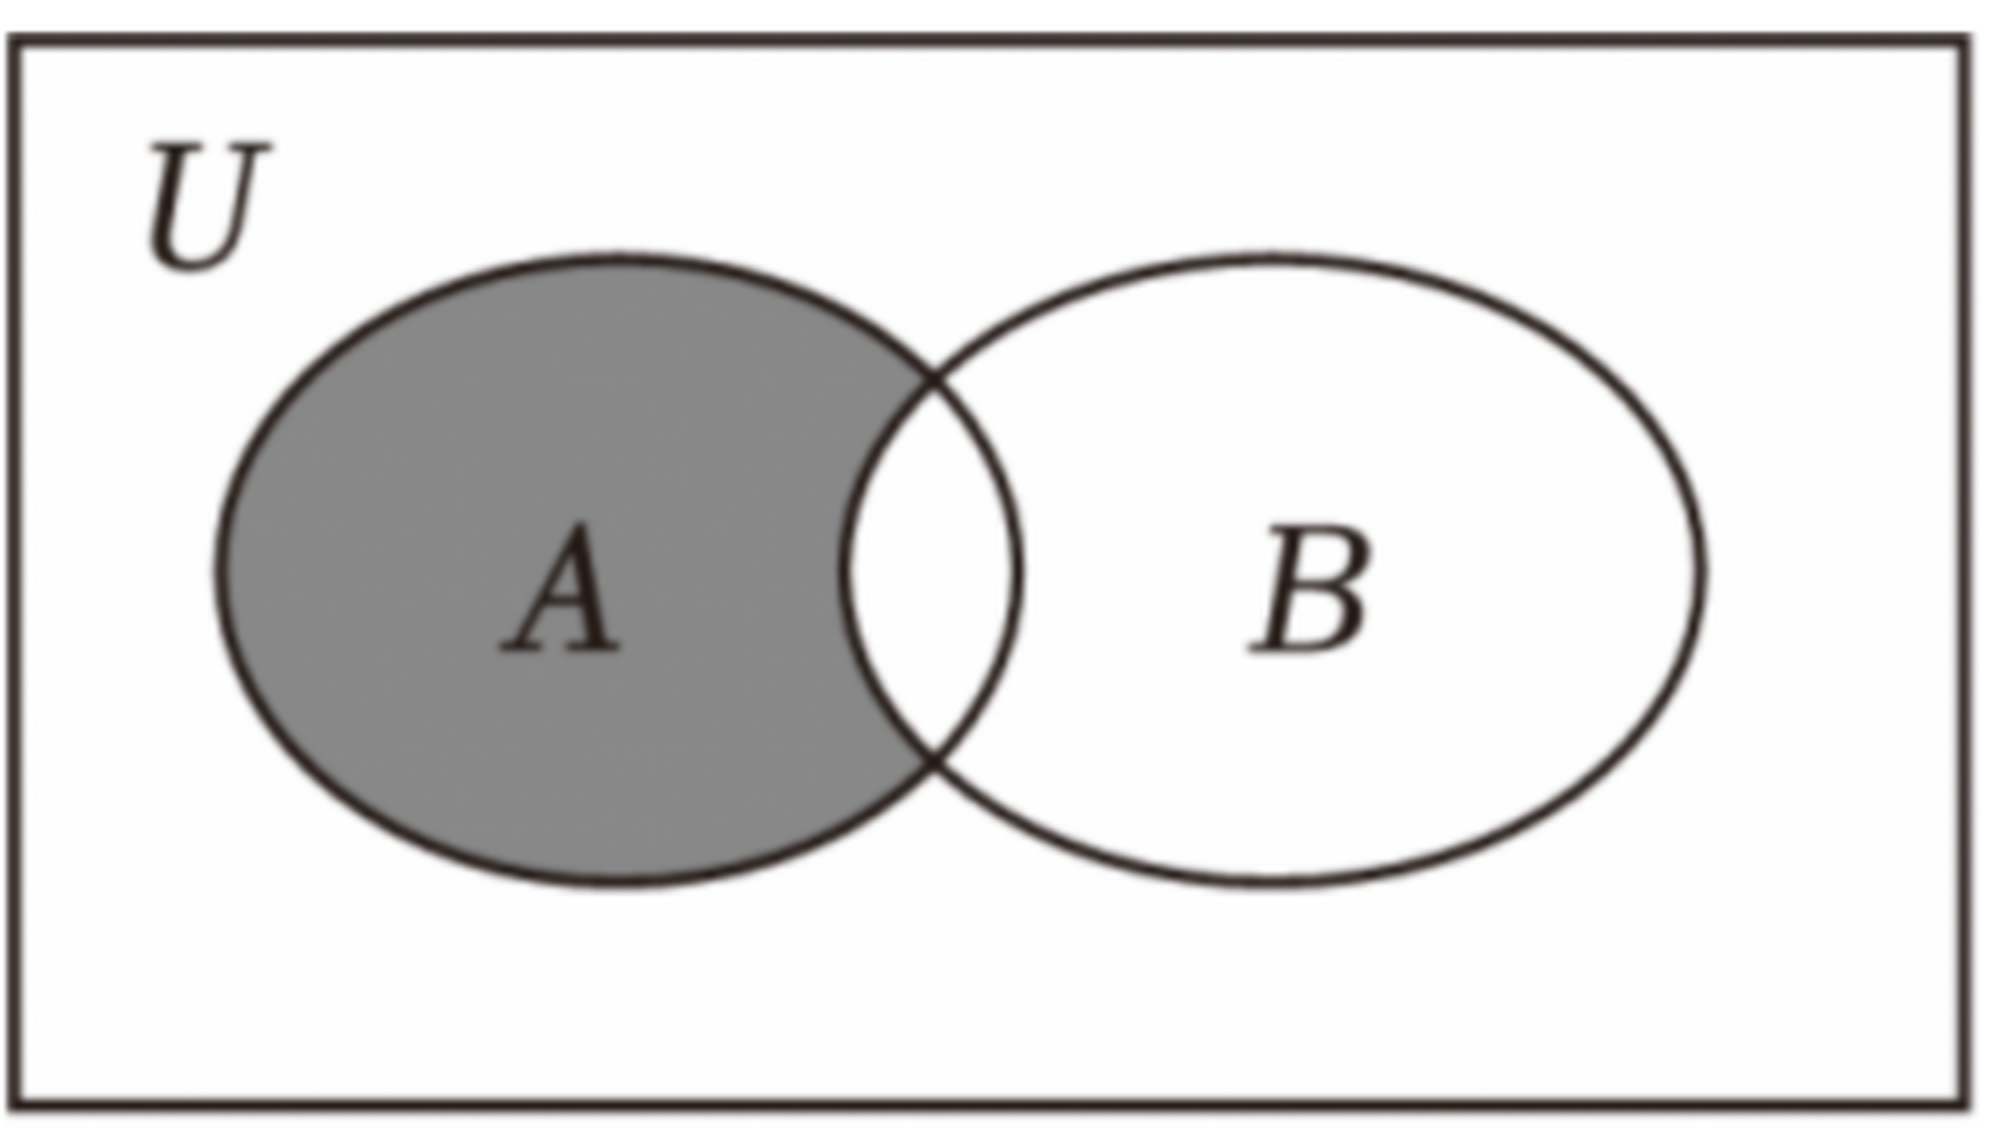
\includegraphics[width=0.34\textwidth]{figures/venn_A_shaded_U.png}
\end{center}

\ans{$A\cap\overline B=(-2,0)$}

\ifanswer
\solbegin
\step{集合 $A=\{x\mid x^2<4\}=(-2,2)$，$B=\{y\mid y=x^2\}=[0,+\infty)$，}
\step{图中阴影部分所表示的集合是 $A\cap\overline B=(-2,0)$.}
\solend
\fi

\item 如图所示，$M$、$P$、$S$ 是 $V$ 的三个子集，则阴影部分所表示的集合是 \blankline[5.4em].

\begin{center}
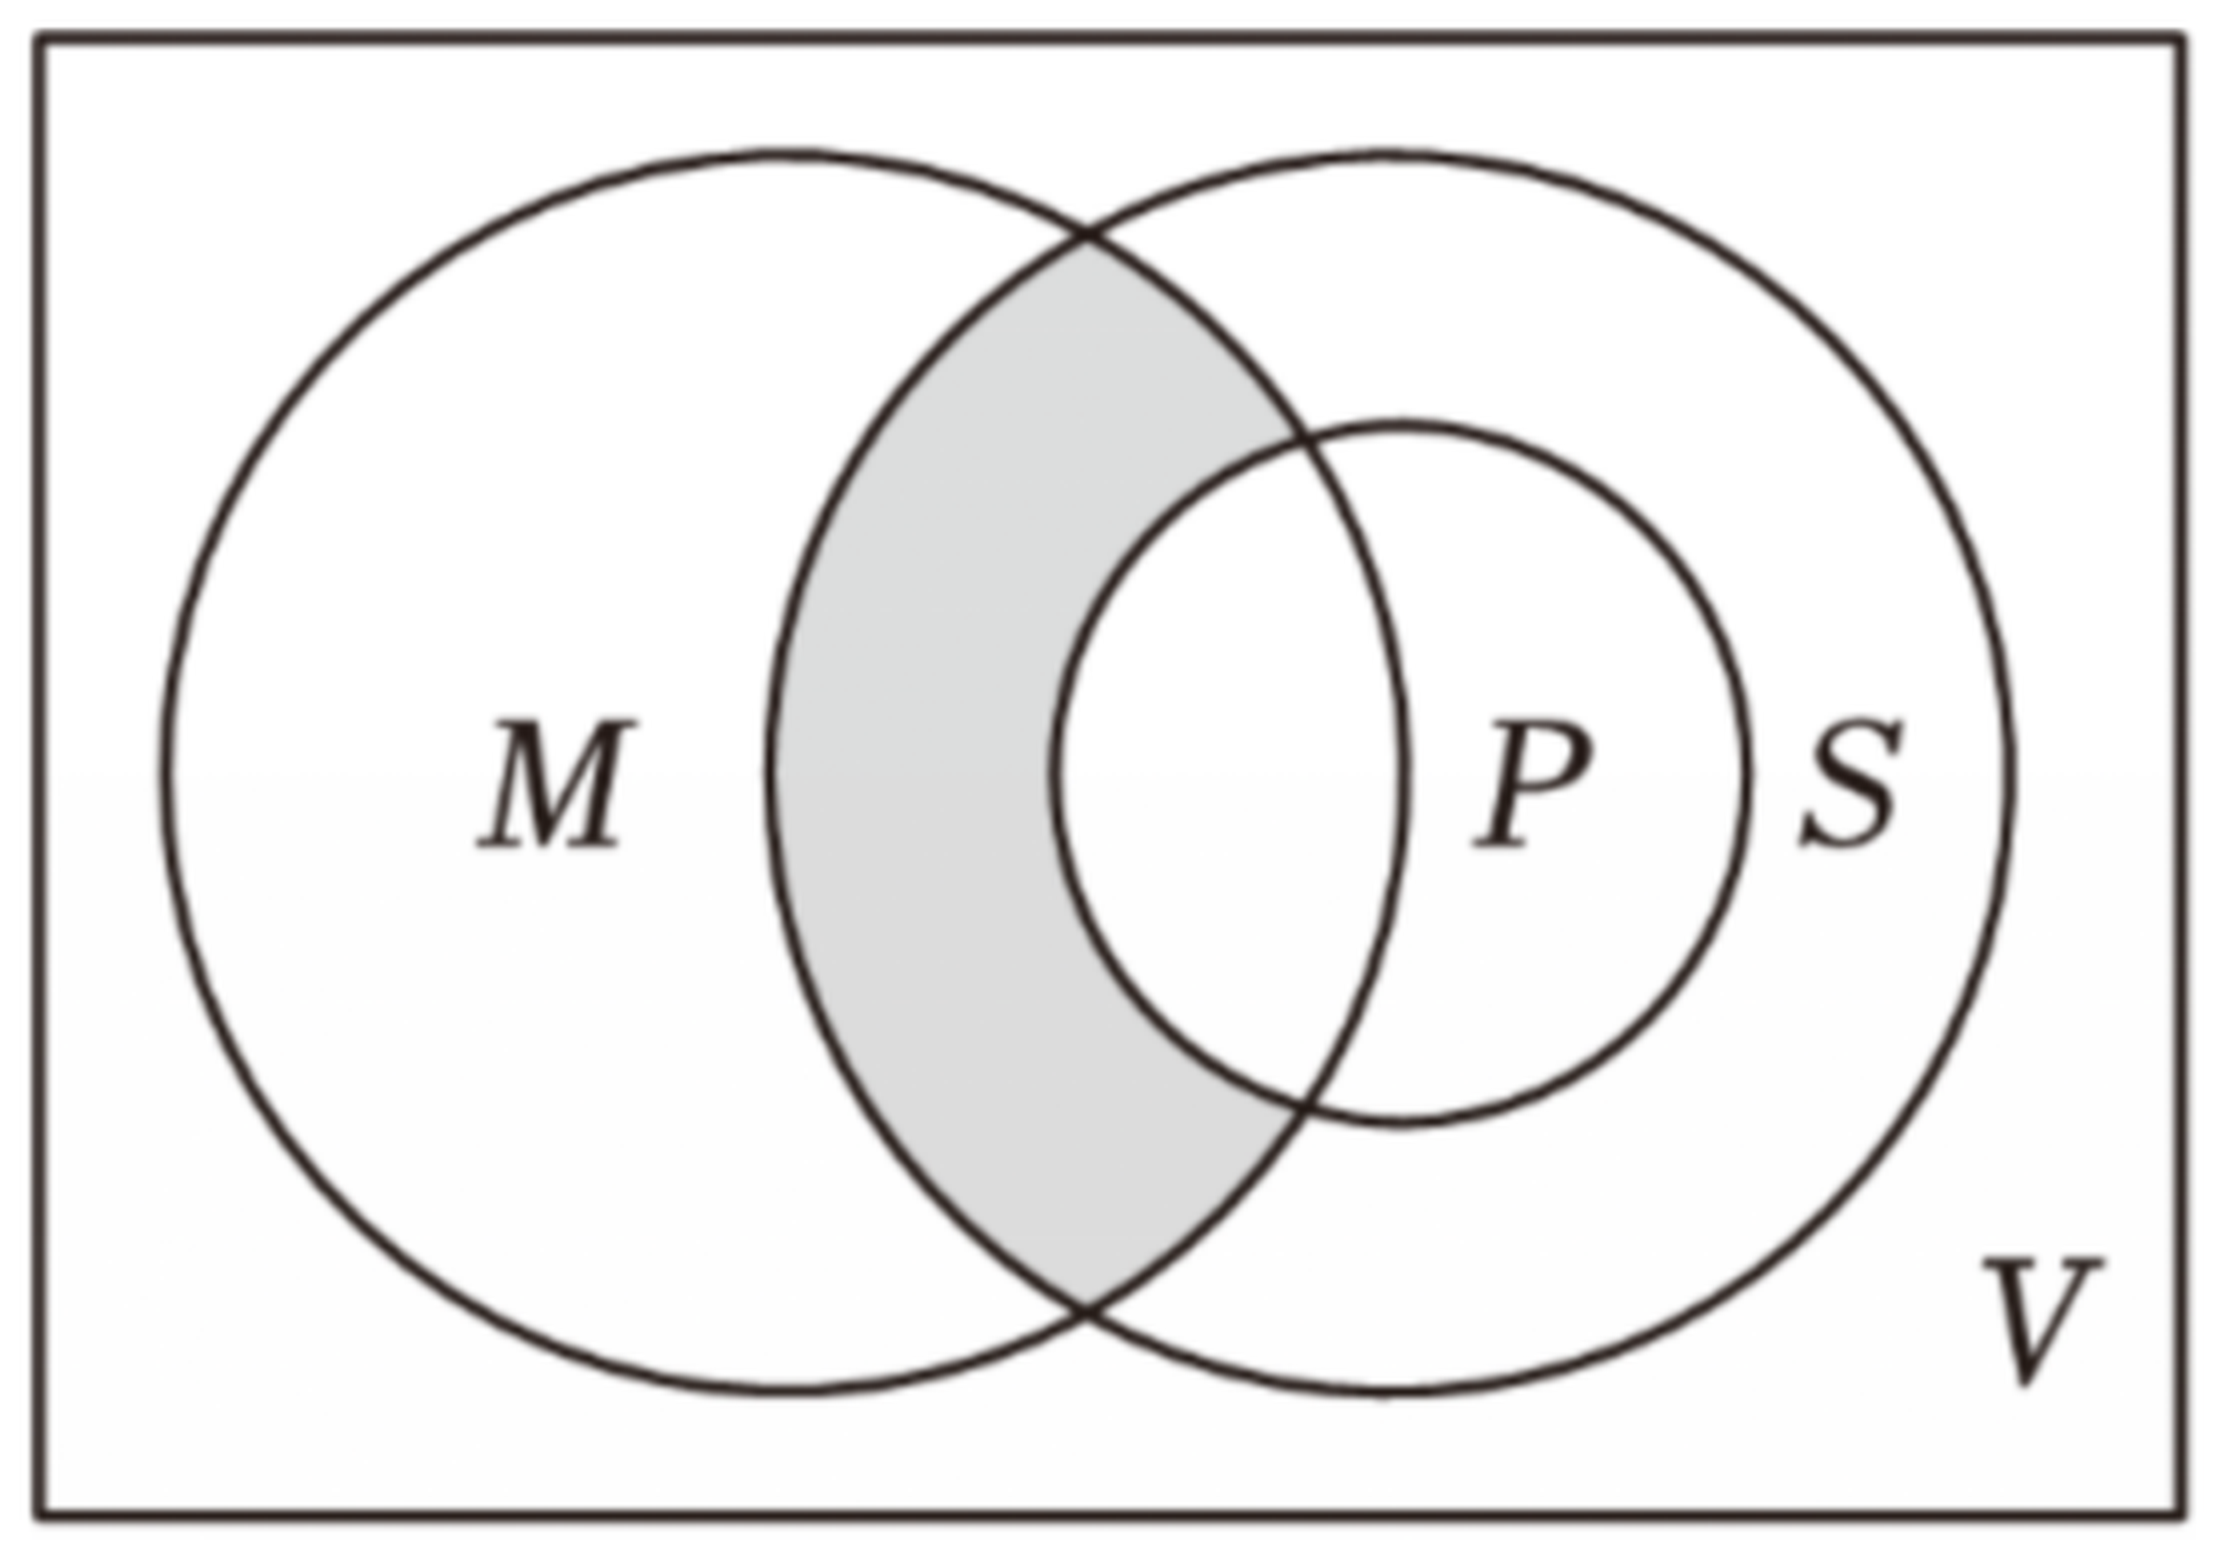
\includegraphics[width=0.38\textwidth]{figures/venn_MPS_V.png}
\end{center}

\ans{$(M\cap S)\cap(\complement_V P)$}

\item 下面六个关系式：① $\varnothing\subseteq\{a\}$；② $a\subseteq\{a\}$；③ $\{a\}\subseteq\{a\}$；④ $\{a\}\in\{a,b\}$；⑤ $a\in\{a,b,c\}$；⑥ $\varnothing\in\{a,b\}$；其中正确的是 \blankline[3.4em].

\ans{①③⑤}

\item 已知集合 $A=\{x\mid -1\le x\le a\}\ne\varnothing$，若 $\{y\mid y=x+1,x\in A\}=\{y\mid y=x^2,x\in A\}$，则实数 $a$ 值为 \blankline[4.4em].

\ans{$0$ 或 $\dfrac{1+\sqrt5}{2}$}

\ifanswer
\solbegin
\step{因为 $A=\{x\mid -1\le x\le a\}\ne\varnothing$，}
\step{所以 $\{y\mid y=x+1,x\in A\}=\{y\mid 0\le y\le a+1\}$，}
\step{$-1\le a\le1$ 时，$\{y\mid y=x^2,x\in A\}=\{y\mid 0\le y\le1\}$，}
\step{$a>1$ 时，$\{y\mid y=x^2,x\in A\}=\{y\mid 0\le y\le a^2\}$，}
\step{① $-1\le a\le1$ 时，$\{y\mid 0\le y\le a+1\}=\{y\mid 0\le y\le1\}$，则 $a+1=1$，解得 $a=0$；}
\step{② $a>1$ 时，$\{y\mid 0\le y\le a+1\}=\{y\mid 0\le y\le a^2\}$，则 $a^2=a+1$，解得 $a=\dfrac{1+\sqrt5}{2}$；}
\step{所以 $a=0$ 或 $\dfrac{1+\sqrt5}{2}$.}
\solend
\fi

\item 设集合 $A=\{(x,y)\mid x+y=22,x>0,y>0,x,y\text{ 均为质数}\}$ 的子集的个数为 \blankline[4.4em].

\ans{$32$}

\ifanswer
\solbegin
\step{集合 $A=\{(x,y)\mid x+y=22,x>0,y>0,x,y\text{ 均为质数}\}$}
\step{$=\{(3,19),(19,3),(5,17),(17,5),(11,11)\}$，则 $A$ 的子集的个数为 $2^5=32$.}
\solend
\fi

% 注：原卷本题题干印作「已知一个有四个数字元素的集合 $S$」；「数字元素」疑为「元素」之衍，
%     但原卷字形确为「数字」二字（已 3× 放大核对过），本稿照录，不代为改写。
\item 已知一个有四个数字元素的集合 $S$，$S$ 的所有子集的元素和（空集的元素和认为是 $0$）的总和为 $16192$，则 $S$ 的元素之和等于 \blankline[4.4em].

\ans{$2024$}

\ifanswer
\solbegin
\step{设 $S=\{a_1,a_2,a_3,a_4\}$，$S$ 的每个元素在所有子集中均出现 $2^3$ 次，}
\step{故 $(a_1+a_2+a_3+a_4)\cdot 2^3=16192$，所以 $a_1+a_2+a_3+a_4=2024$，}
\step{故 $S$ 的元素之和等于 $2024$.}
\solend
\fi

\item 设 $A$ 是非空数集，若对任意 $x$、$y\in A$，都有 $x+y\in A$、$xy\in A$，则称 $A$ 具有性质 $P$，给出以下命题：

①若 $A$ 具有性质 $P$，则 $A$ 可以是有限集；

②若 $A$ 具有性质 $P$，且 $A\ne\R$，则 $\overline A$ 具有性质 $P$；

③若 $A_1$、$A_2$ 具有性质 $P$，且 $A_1\cap A_2\ne\varnothing$，则 $A_1\cap A_2$ 具有性质 $P$；

④若 $A_1$、$A_2$ 具有性质 $P$，则 $A_1\cap A_2$ 具有性质 $P$.

其中所有真命题的序号是 \blankline[4.4em].

\ans{①③}

\ifanswer
\solbegin
\step{对于①，取集合 $A=\{0,1\}$ 具有性质 $P$，故 $A$ 可以是有限集，故①正确；}
\step{对于③，取 $x$、$y\in A_1\cap A_2$，则 $x\in A_1$，$x\in A_2$，$y\in A_1$，$y\in A_2$，}
\step{又 $A_1$、$A_2$ 具有性质 $P$，所以 $x+y\in A_1$，$xy\in A_1$，$x+y\in A_2$，$xy\in A_2$，}
\step{所以 $x+y\in A_1\cap A_2$，$xy\in A_1\cap A_2$，所以 $A_1\cap A_2$ 具有性质 $P$，故③正确；}
\step{对于④，取 $A_1=\{x\mid x=2k,k\in\Z\}$，$A_2=\{x\mid x=3k,k\in\Z\}$，$2\in A_1$，$3\in A_2$，}
\step{但 $2+3\notin A_1\cup A_2$，故④错误；}
\step{对于②，若 $A$ 具有性质 $P$，且 $A\ne\R$，假设 $\overline A$ 也具有性质 $P$，}
\step{设 $0\in A$，在 $\overline A$ 中任取一个 $x$，$x\ne0$，此时可证得 $-x\in A$，}
\step{否则若 $-x\in\overline A$，由于 $\overline A$ 也具有性质 $P$，则 $x+(-x)=0\in\overline A$，}
\step{与 $0\in A$ 矛盾，故 $-x\in A$，}
\step{由于 $A$ 具有性质 $P$，$\overline A$ 也具有性质 $P$，所以 $(-x)^2\in A$，$x^2\in\overline A$，}
\step{而 $(-x)^2=x^2$，这与 $A\cap\overline A=\varnothing$ 矛盾，}
\step{故当 $0\in A$ 且 $A$ 具有性质 $P$ 时，则 $\overline A$ 不具有性质 $P$，}
\step{同理当 $0\in\overline A$ 时，也可以类似推出矛盾，故②错误.}
\step{故正确的是①③.}
\solend
\fi

\item 已知 $S=\{1,2,3,4,5\}$，$A=\{1,2,5\}$，$T=\{t_1,t_2\}\subseteq S$，记 $A_1=\{x\mid x=a+t_1,a\in A,t_1\in T\}$，$A_2=\{x\mid x=b+t_2,b\in A,t_2\in T\}$，若 $A_1\cap A_2=\varnothing$，则集合 $T$ 为 \blankline[5.4em].

\ans{$T=\{1,3\}$ 或 $T=\{2,4\}$ 或 $T=\{3,5\}$}

\ifanswer
\solbegin
\step{若 $A_1\cap A_2=\varnothing$，即 $a+t_1\ne b+t_2$，则 $t_1-t_2\ne a-b$，其中 $a$、$b\in A$，}
\step{否则 $t_1+a=t_2+b$，$A_1\cap A_2\ne\varnothing$，}
\step{又 $S=\{1,2,3,4,5\}$，$A=\{1,2,5\}$，$T=\{t_1,t_2\}\subseteq S$，}
\step{$2-1=1$，$5-2=3$，$5-1=4$，则 $t_1$、$t_2$ 相差 $2$，}
\step{所以 $T=\{1,3\}$ 或 $T=\{2,4\}$ 或 $T=\{3,5\}$.}
\solend
\fi

\end{enumerate}

\bigsec{二、解答题}

\begin{enumerate}
\setcounter{enumi}{13}

\item 设集合 $P=\{1,2,3,m\}$，$Q=\{3,m^2\}$，且 $\overline P\cap Q=\varnothing$，求实数 $m$ 的值组成的集合.

\ans{$\{-1,0,\pm\sqrt2\}$}

\ansspace[5]

\ifanswer
\solbegin
\step{因为 $\overline P\cap Q=\varnothing$，所以 $Q\subseteq P$，所以 $m^2=1$ 或 $m^2=2$ 或 $m^2=m$，}
\step{考虑互异性，得 $m=-1$ 或 $m=\pm\sqrt2$ 或 $m=0$，}
\step{所以实数 $m$ 的值组成的集合为 $\{-1,0,\pm\sqrt2\}$.}
\solend
\fi

\item 若集合 $A=(-\infty,2]$，$B=\{x\mid kx+1<0,k\in\R\}$，$A\cap B=\varnothing$，求实数 $k$ 的取值范围.

\ans{$\left[-\dfrac12,0\right]$}

\ansspace[5]

\ifanswer
\solbegin
\step{若 $B=\varnothing$，则 $k=0$，符合题意，}
\step{若 $B\ne\varnothing$，当 $k>0$ 时，$B=\left(-\infty,-\dfrac1k\right)$，$A\cap B\ne\varnothing$，不合题意；}
\step{当 $k<0$ 时，$B=\left(-\dfrac1k,+\infty\right)$，由 $A\cap B=\varnothing$ 得 $-\dfrac1k\ge2$，即 $-\dfrac12\le k<0$，}
\step{故 $k$ 的取值范围是 $\left[-\dfrac12,0\right]$.}
\solend
\fi

\item 已知集合 $A=\{-4,2a-1,a^2\}$，$B=\{a-5,1-a,9\}$，分别求适合下列条件的 $a$ 的值.

% 两个小问不许与题干分家：试卷版第 2 页页末原本正好把 (1) 留在页底、(2) 翻到次页，
% 与 2026-09-15 修的三类难看切页同源，故在这里也加 \keepwithprev 守卫（三版都生效）。
\keepwithprev
（1）$9\in(A\cap B)$；

\keepwithprev
（2）$\{9\}=A\cap B$.

\ans{（1）$a=5$ 或 $a=-3$；（2）$a=-3$}

\ansspace[5]

\ifanswer
\solbegin
\stepm{（1）}{$9\in(A\cap B)$，所以 $9\in A$，}
\step{当 $2a-1=9$ 时，$a=5$，当 $a^2=9$ 时，即 $a=\pm3$，}
% 注：原卷此句结论印作「所以 $a$ 的值为 $5\backslash-3$」——「\」应是顿号之误，
%     本稿照录原卷字形（见文件头「原卷存疑」②）；按文意即 $a=5$ 或 $a=-3$。
\step{当 $a=3$ 时，$a-5=1-a$ 舍去，所以 $a$ 的值为 $5\backslash-3$.}
\stepm{（2）}{结合（1）的结论：}
\step{当 $2a-1=9$ 即 $a=5$ 时，$1-a=-4$，$\{9\}\ne(A\cap B)$，}
\step{当 $a^2=9$ 时，即 $a=\pm3$，当 $a=3$ 时，$a-5=1-a$ 舍去，}
\step{所以 $a$ 的值为 $-3$.}
\solend
\fi

\item 已知集合 $M=\{a,ab,a-b\}$，$N=\{0,|a|,b\}$，且 $M=N$，求实数 $a$、$b$ 的值.

\ans{$a=b=-1$}

\ansspace[5]

\ifanswer
\solbegin
\step{由集合元素的互异性，得 $a\ne0$，且 $b\ne0$，所以 $a-b=0$，即 $a=b$，}
\step{所以 $ab=|a|$，又由 $|a|\ne b=a$，得 $a<0$，故 $a=b=-1$.}
\solend
\fi

\item 已知集合 $A=\{x\mid -2<x<7\}$，$B=\{x\mid m+1\le x\le 2m-1\}$.

\keepwithprev
（1）当 $m=4$ 时，求 $A\cap B$、$A\cup B$；

\keepwithprev
（2）若 $A\cap B=B$，求实数 $m$ 的取值范围.

\ans{（1）$A\cap B=[5,7)$，$A\cup B=(-2,7]$；（2）$(-\infty,4)$}

\ansspace[5]

\ifanswer
\solbegin
\stepm{（1）}{当 $m=4$ 时，得集合 $A=\{x\mid -2<x<7\}$，$B=\{x\mid 5\le x\le7\}$，}
\step{得 $A\cap B=[5,7)$，$A\cup B=(-2,7]$.}
\stepm{（2）}{由 $A\cap B=B$ 得 $B\subseteq A$，}
\step{①当 $B=\varnothing$ 时，得 $m+1>2m-1$，解得 $m<2$；}
\step{②当 $B\ne\varnothing$ 时，得 $\begin{cases}m+1>-2\\ 2m-1<7\\ m+1\le2m-1\end{cases}$，解得 $2\le m<4$；}
\step{综上，实数 $m$ 的取值范围是 $(-\infty,4)$.}
\solend
\fi

\item 若集合 $A=\{x\mid x^2+5x-6=0\}$，$B=\{x\mid x^2+2(m+1)x+m^2-3=0\}$.

\keepwithprev
（1）当 $m=0$ 时，求集合 $A\cup B$；

\keepwithprev
（2）若 $A\cap B=B$，求实数 $m$ 的取值范围.

\ans{（1）$A\cup B=\{1,-6,-3\}$；（2）$\{m\mid m\le-2\}$}

\ansspace[5]

\ifanswer
\solbegin
\stepm{（1）}{由题意得，集合 $A=\{x\mid x^2+5x-6=0\}=\{1,-6\}$，}
\step{当 $m=0$ 时，$B=\{x\mid x^2+2x-3=0\}=\{1,-3\}$，}
\step{所以 $A\cup B=\{1,-6,-3\}$；}
\stepm{（2）}{由（1）得集合 $A=\{1,-6\}$，$B=\{x\mid x^2+2(m+1)x+m^2-3=0\}$，}
\step{若 $A\cap B=B$ 得 $B\subseteq A$，所以 $B=\varnothing$ 或 $\{-6\}$ 或 $\{1\}$ 或 $\{1,-6\}$，}
\step{当 $B=\varnothing$ 时，$\Delta=4(m+1)^2-4(m^2-3)<0$，解得 $m<-2$，}
\step{当 $B=\{-6\}$ 时，则 $\begin{cases}\Delta=4(m+1)^2-4(m^2-3)=0\\ 36-12(m+1)+m^2-3=0\end{cases}$，无解，}
\step{当 $B=\{1\}$ 时，则 $\begin{cases}\Delta=4(m+1)^2-4(m^2-3)=0\\ 1+2(m+1)+m^2-3=0\end{cases}$，解得 $m=-2$，}
\step{当 $B=\{1,-6\}$ 时，则 $\begin{cases}\Delta=4(m+1)^2-4(m^2-3)>0\\ 1+(-6)=-2(m+1)\\ 1\times(-6)=m^2-3\end{cases}$，无解，}
\step{综上所述，实数 $m$ 的取值范围为 $\{m\mid m\le-2\}$.}
\solend
\fi

% 压轴题：其后已无内容，故作答区全用可丢弃胶水（\ansspace*），并在题目前先量一下版面。
\ansneed{8cm}
\item 对于点集 $A=\{(x,y)\mid x=m,y=-3x+2,m\in\N,m\ge1\}$，$B=\{(x,y)\mid x=n,y=a(x^2-x+1),n\in\N,n\ge1\}$，是否存在非零整数 $a$，使得 $A\cap B\ne\varnothing$？

\ans{$a=-1$}

\ansspace*[10]

\ifanswer
\solbegin
\step{当 $A\cap B\ne\varnothing$ 时，$-3x+2=a(x^2-x+1)$，}
\step{$ax^2+(3-a)x+a-2=0$ ①有正整数解，}
\step{所以 $\Delta=(3-a)^2-4a(a-2)=-3a^2+2a+9$ 是平方数，}
\step{所以 $3a^2-2a-9\le0$，$\dfrac{1-2\sqrt7}{3}\le a\le\dfrac{1+2\sqrt7}{3}$，$a\ne0$，$a\in\Z$，}
\step{所以 $a=\pm1$ 或 $a=2$，}
\step{$a=-1$ 时 $\Delta=4$，这时①变为 $-x^2+4x-3=0$，解得 $x_1=1$，$x_2=3$，}
\step{$A\cap B=\{(1,-1),(3,-7)\}$.}
\step{$a=1$ 时 $\Delta=8$，不是平方数.}
\step{$a=2$ 时 $\Delta=1$，这时①变为 $2x^2+x=0$，没有正整数解.}
\step{所以 $a=-1$.}
\solend
\fi

\end{enumerate}

\end{document}
"
% 紧凑版：xelatex "\def\iscompact{1}% 高一19_延安中学_周末作业2.tex —— 高一上数学「2026-2027 年延安中学高一上周末作业 2」（试卷版/答案版）
% 试卷版：xelatex 高一19_延安中学_周末作业2.tex
% 答案版：xelatex "\def\isanswer{1}\input{高一19_延安中学_周末作业2.tex}"
% 紧凑版：xelatex "\def\iscompact{1}\input{高一19_延安中学_周末作业2.tex}"
%
% 原始材料是微信公众号图文（公众号「魔都数学加油站」，作者署名「破晓」，
% 原文链接 https://mp.weixin.qq.com/s/tHqWSV1StO5SHSXXQ4jeUA），正文为 6 张 PNG 页；
% 原文本身就是一份**讲评版**——题目下方直接印出【答案】或【解析】。本稿把答案与解析
% 移到答案版，试卷版即一张干净的空卷；试题文字、答案与解析均照原卷录入。
%
% 与原卷的排版差异（均已在 README「说明」中交代）：
%   ① 原文自**第 3 题**起（第 1、2 题未在该文发布），源码里以 \setcounter{enumi}{2} 起编；
%      全卷只有「一、填空题」「二、解答题」两节，无选择题；
%   ② 原卷本就印有两个分节标题（已在原图上逐页放大核对过），本稿照原卷分节，只把标题改排
%      成全稿统一的「大节标题」样式；
%   ③ 原卷的实数集、整数集、自然数集符号作正体 $R$、$Z$、$N$（第 15 题作粗体 $\mathbf{R}$，
%      第 20 题有 $N$ 与斜体 $Z$），本稿按全稿惯例统一写作 $\R$、$\Z$、$\N$；
%   ④ 第 4 题的韦恩图在原卷里印在【解析】右侧（题干并无「如图」二字），故本稿把该图放进
%      答案版的解析块内（`figures/venn_AB_survey_50_x.png`）；第 6、7 题的韦恩图是**题干图**
%      （题干作「图中阴影部分所表示的集合」），两版都排（`figures/venn_A_shaded_U.png`、
%      `figures/venn_MPS_V.png`）。三张图都取自原卷截图、4× LANCZOS 放大，不用 TikZ 手绘；
%   ⑤ 本卷也是「讲评版」，解析按全稿统一的 \solbegin/\step 分步重排（原卷为连续段落），
%      分步不改一字，只断句、断行；
%   ⑥ 标题前缀照**原卷**作「2026--2027 年…」（原卷标题即作「2026-2027年延安中学高一上周末
%      作业 2」）。同校的 高一06 作「学年度」——那是 高一02—高一09 那一批入库时统一改的；
%      后续入库的卷（高一10—高一17 与本卷）一律照原卷保留「年」，未强改，故同校两卷前缀不同。
%
% 原卷存疑两处（已逐处放大到能看清字形后核对，本稿照录并加注，见各题下的 `%` 注）：
%   （另有第三处「第 12 题【解析】末句」原先记作存疑，2026-09-26 第二轮核对放大后发现
%     原卷印的是「$0\in\overline A$」——A 上确有横杠，是本稿当初漏抄了 $\overline{}$；
%     已按原卷补回，故该条从存疑清单里删去，不计为原卷问题。）
%   ① 第 11 题题干印作「已知一个有四个数字元素的集合 $S$」，「数字元素」疑为「元素」之衍；
%   ② 第 16 题 (1) 结论印作「$a$ 的值为 $5\backslash-3$」，其中的「\」应是顿号之误
%      （由 (2) 的结论「$a$ 的值为 $-3$」可反推，(1) 的答案是 $5$ 或 $-3$）；

% 本篇在公众号「魔都数学加油站」连载里的编号是「27学年高一19」，本地编号与之对齐（高一19）；
% 对应关系见 README「与公众号连载号的对照表」。
\documentclass[a4paper,11pt]{article}
\usepackage{common}

\begin{document}

\examtitlest{2026--2027 年延安中学高一上周末作业 2}{集合与常用逻辑用语}

\bigsec{一、填空题}

\begin{enumerate}
% 原卷填空题从第 3 题起（1、2 未在该文中发布），须与解答题的 \setcounter{enumi}{13} 对齐
\setcounter{enumi}{2}
\item 已知全集 $U=\{1,2,3,4,5\}$，$M=\{1,2\}$，$P=\{1,3,5\}$，则 $M\cap\overline P=$ \blankline[4.4em].

\ans{$\{2\}$}

\item 某公司共有 $50$ 人，此次组织参加社会公益活动，其中参加 $A$ 项公益活动的有 $28$ 人，参加 $B$ 项公益活动的有 $33$ 人，且 $A$、$B$ 两项公益活动都不参加的人数比都参加的人数的三分之一多 $1$ 人，则只参加 $A$ 项不参加 $B$ 项的人数是 \blankline[4.4em].

\ans{$10$}

\ifanswer
\solbegin
\step{如图所示，设 $A$、$B$ 两项公益活动都参加的有 $x$ 人，}
\begin{center}
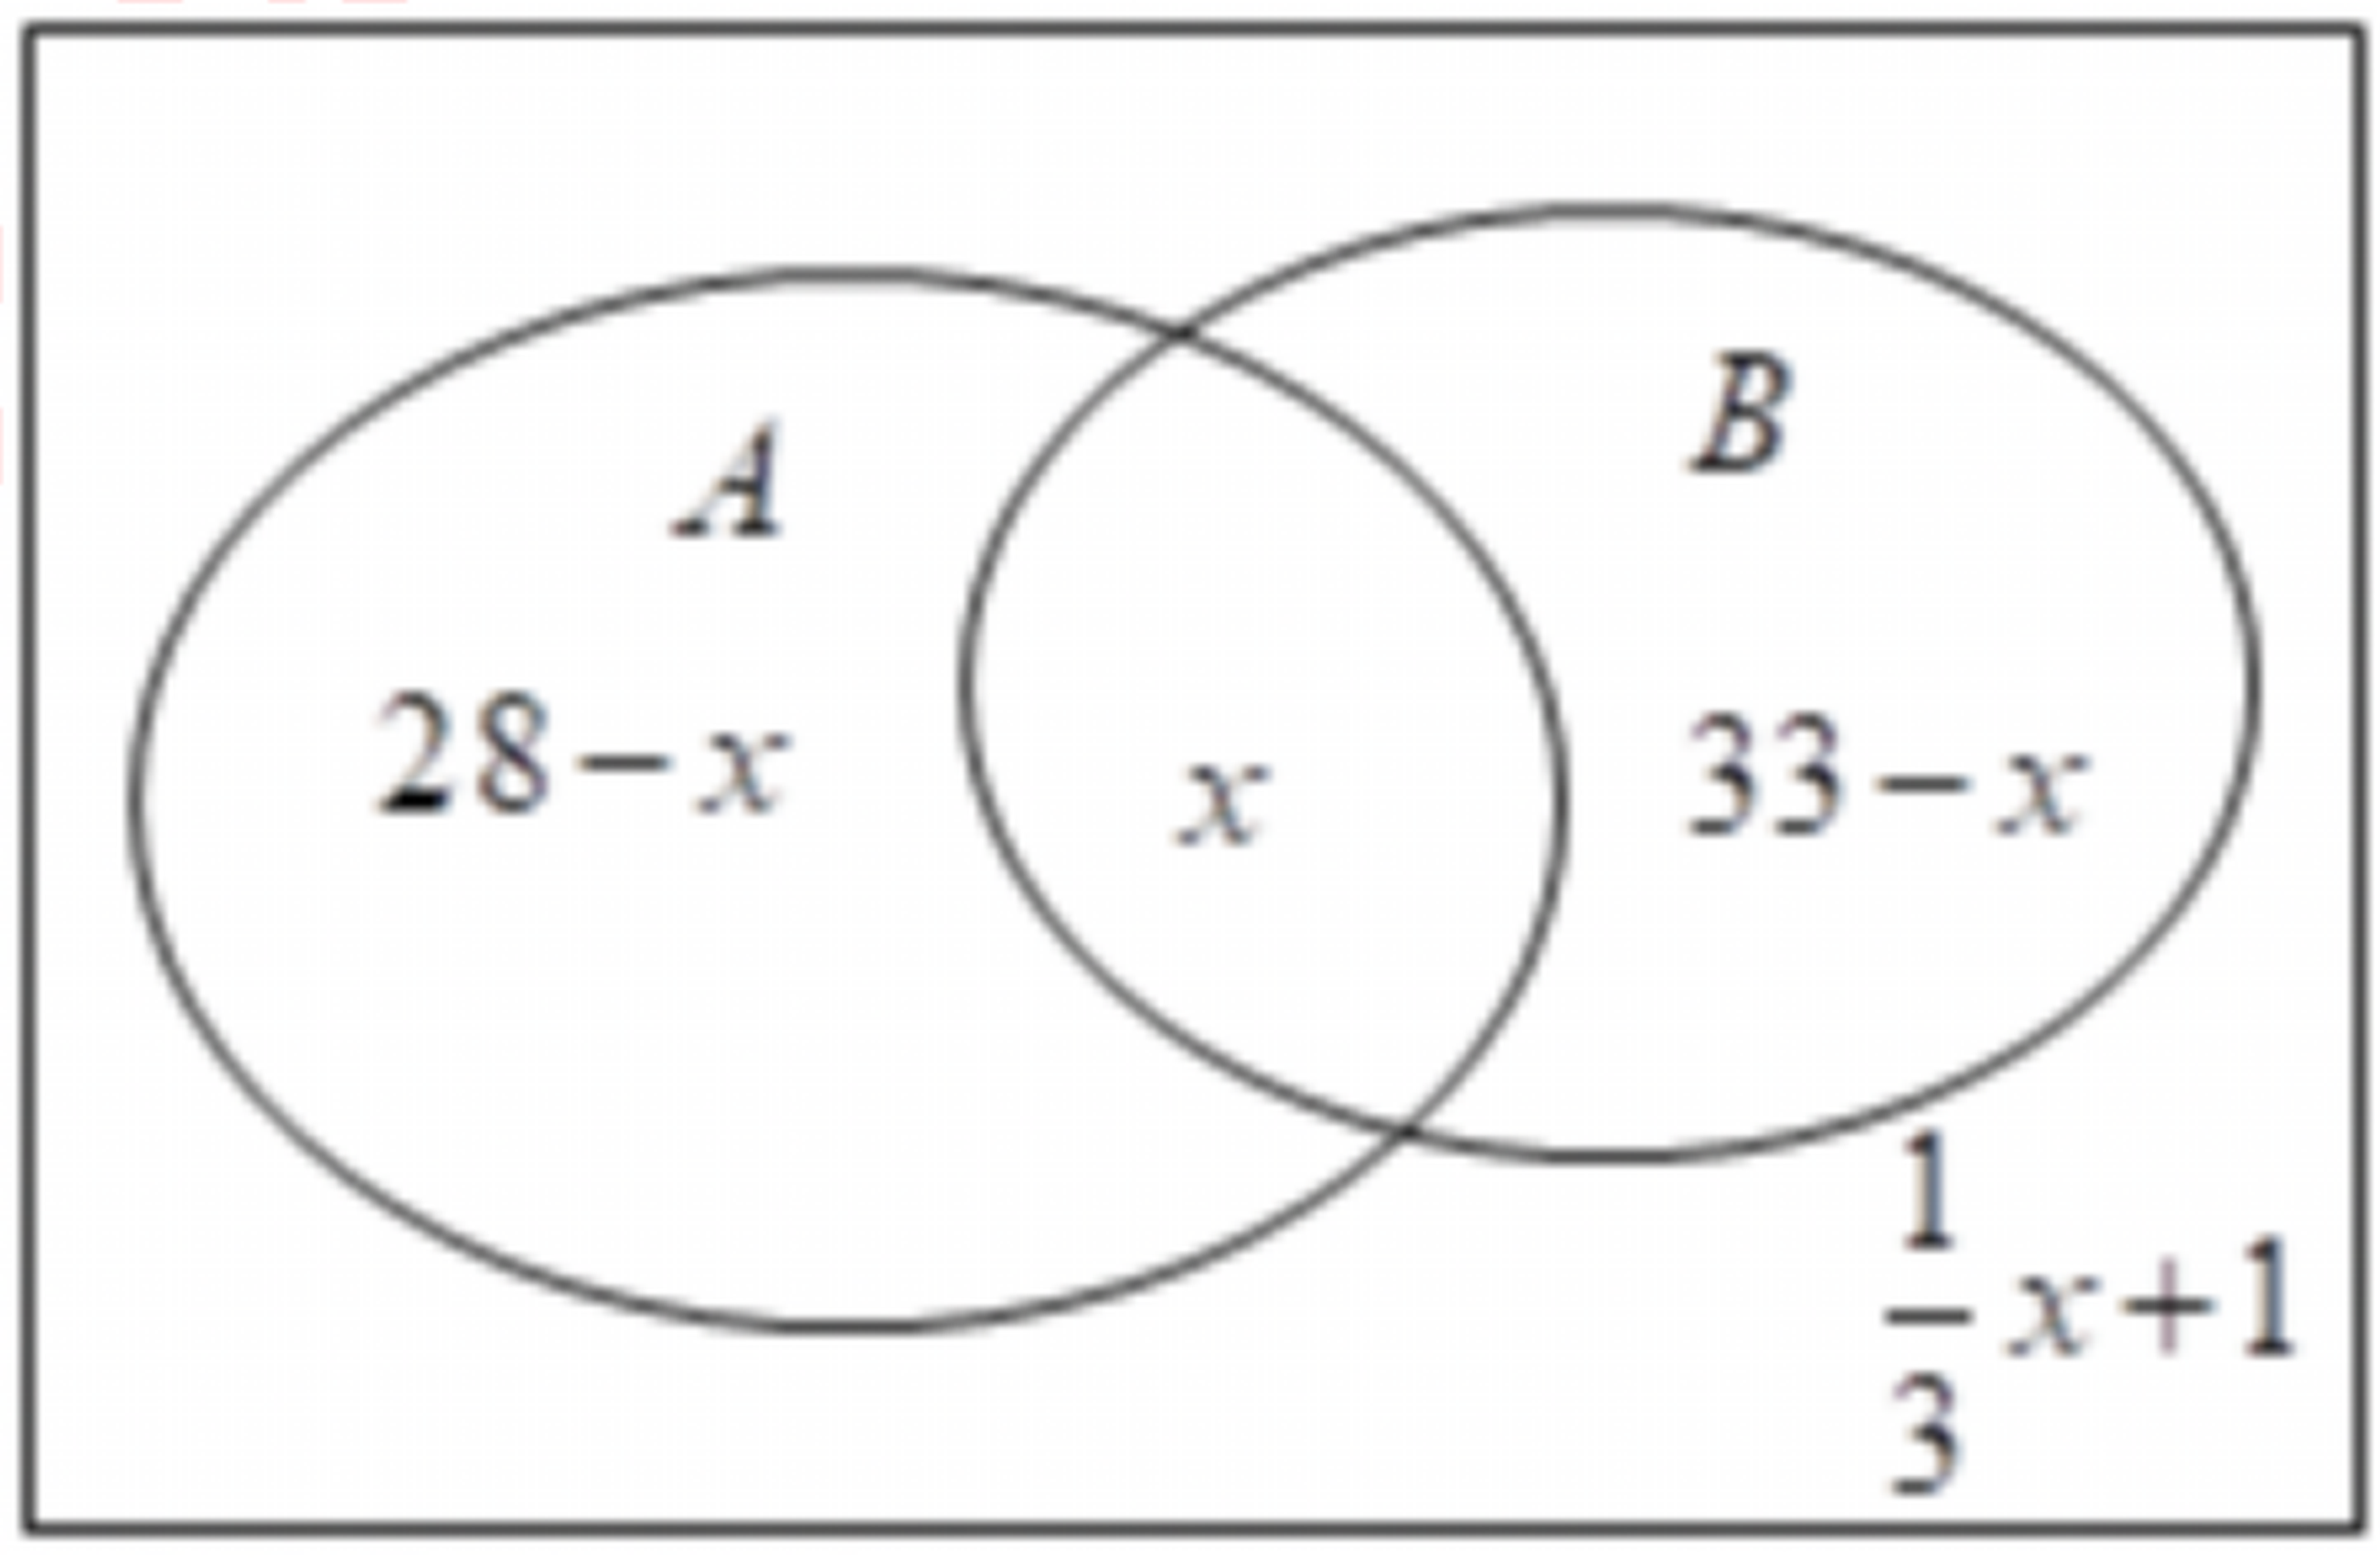
\includegraphics[width=0.42\textwidth]{figures/venn_AB_survey_50_x.png}
\end{center}
\step{则仅参加 $A$ 项的有 $(28-x)$ 人，仅参加 $B$ 项的有 $(33-x)$ 人，}
\step{$A$、$B$ 两项公益活动都不参加的有 $\left(\dfrac13x+1\right)$ 人，}
\step{由题意得 $x+(28-x)+(33-x)+\left(\dfrac13x+1\right)=50$，解得 $x=18$，}
\step{所以只参加 $A$ 项不参加 $B$ 项的有 $28-18=10$ 人.}
\solend
\fi

\item 设集合 $A=\{x\mid x^2-3x+2=0\}$，则满足 $A\cup B=\{0,1,2\}$ 的集合 $B$ 的个数是 \blankline[4.4em].

\ans{$4$}

\ifanswer
\solbegin
\step{$A=\{x\mid x^2-3x+2=0\}=\{x\mid x=1\text{ 或 }x=2\}=\{1,2\}$，}
\step{若 $A\cup B=\{0,1,2\}$，则 $0\in B$，}
\step{则 $B=\{0\},\{0,2\},\{1,0\},\{0,1,2\}$，共 $4$ 个.}
\solend
\fi

\item 已知全集 $U=\R$，集合 $A=\{x\mid x^2<4\}$，$B=\{y\mid y=x^2\}$，则图中阴影部分所表示的集合为 \blankline[4.4em].

\begin{center}
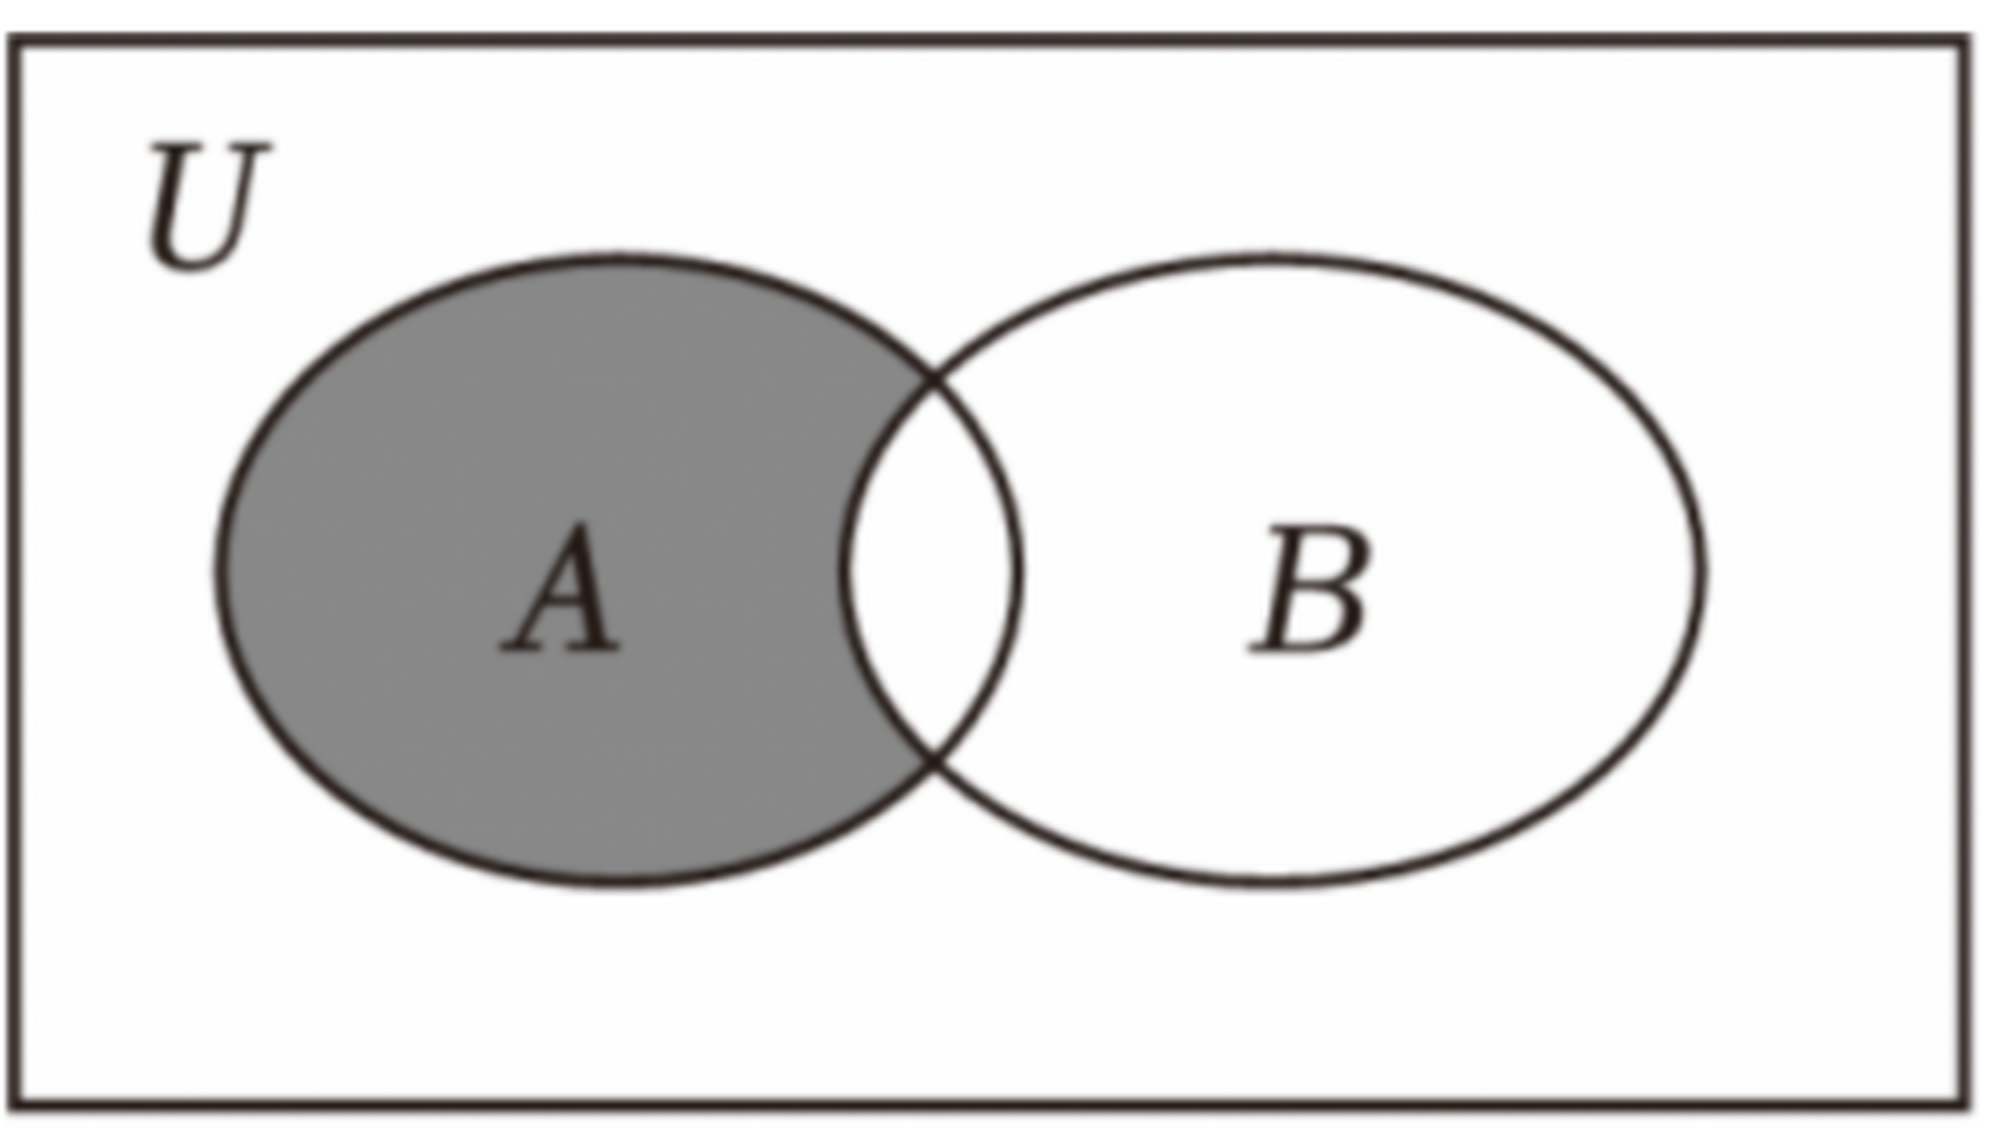
\includegraphics[width=0.34\textwidth]{figures/venn_A_shaded_U.png}
\end{center}

\ans{$A\cap\overline B=(-2,0)$}

\ifanswer
\solbegin
\step{集合 $A=\{x\mid x^2<4\}=(-2,2)$，$B=\{y\mid y=x^2\}=[0,+\infty)$，}
\step{图中阴影部分所表示的集合是 $A\cap\overline B=(-2,0)$.}
\solend
\fi

\item 如图所示，$M$、$P$、$S$ 是 $V$ 的三个子集，则阴影部分所表示的集合是 \blankline[5.4em].

\begin{center}
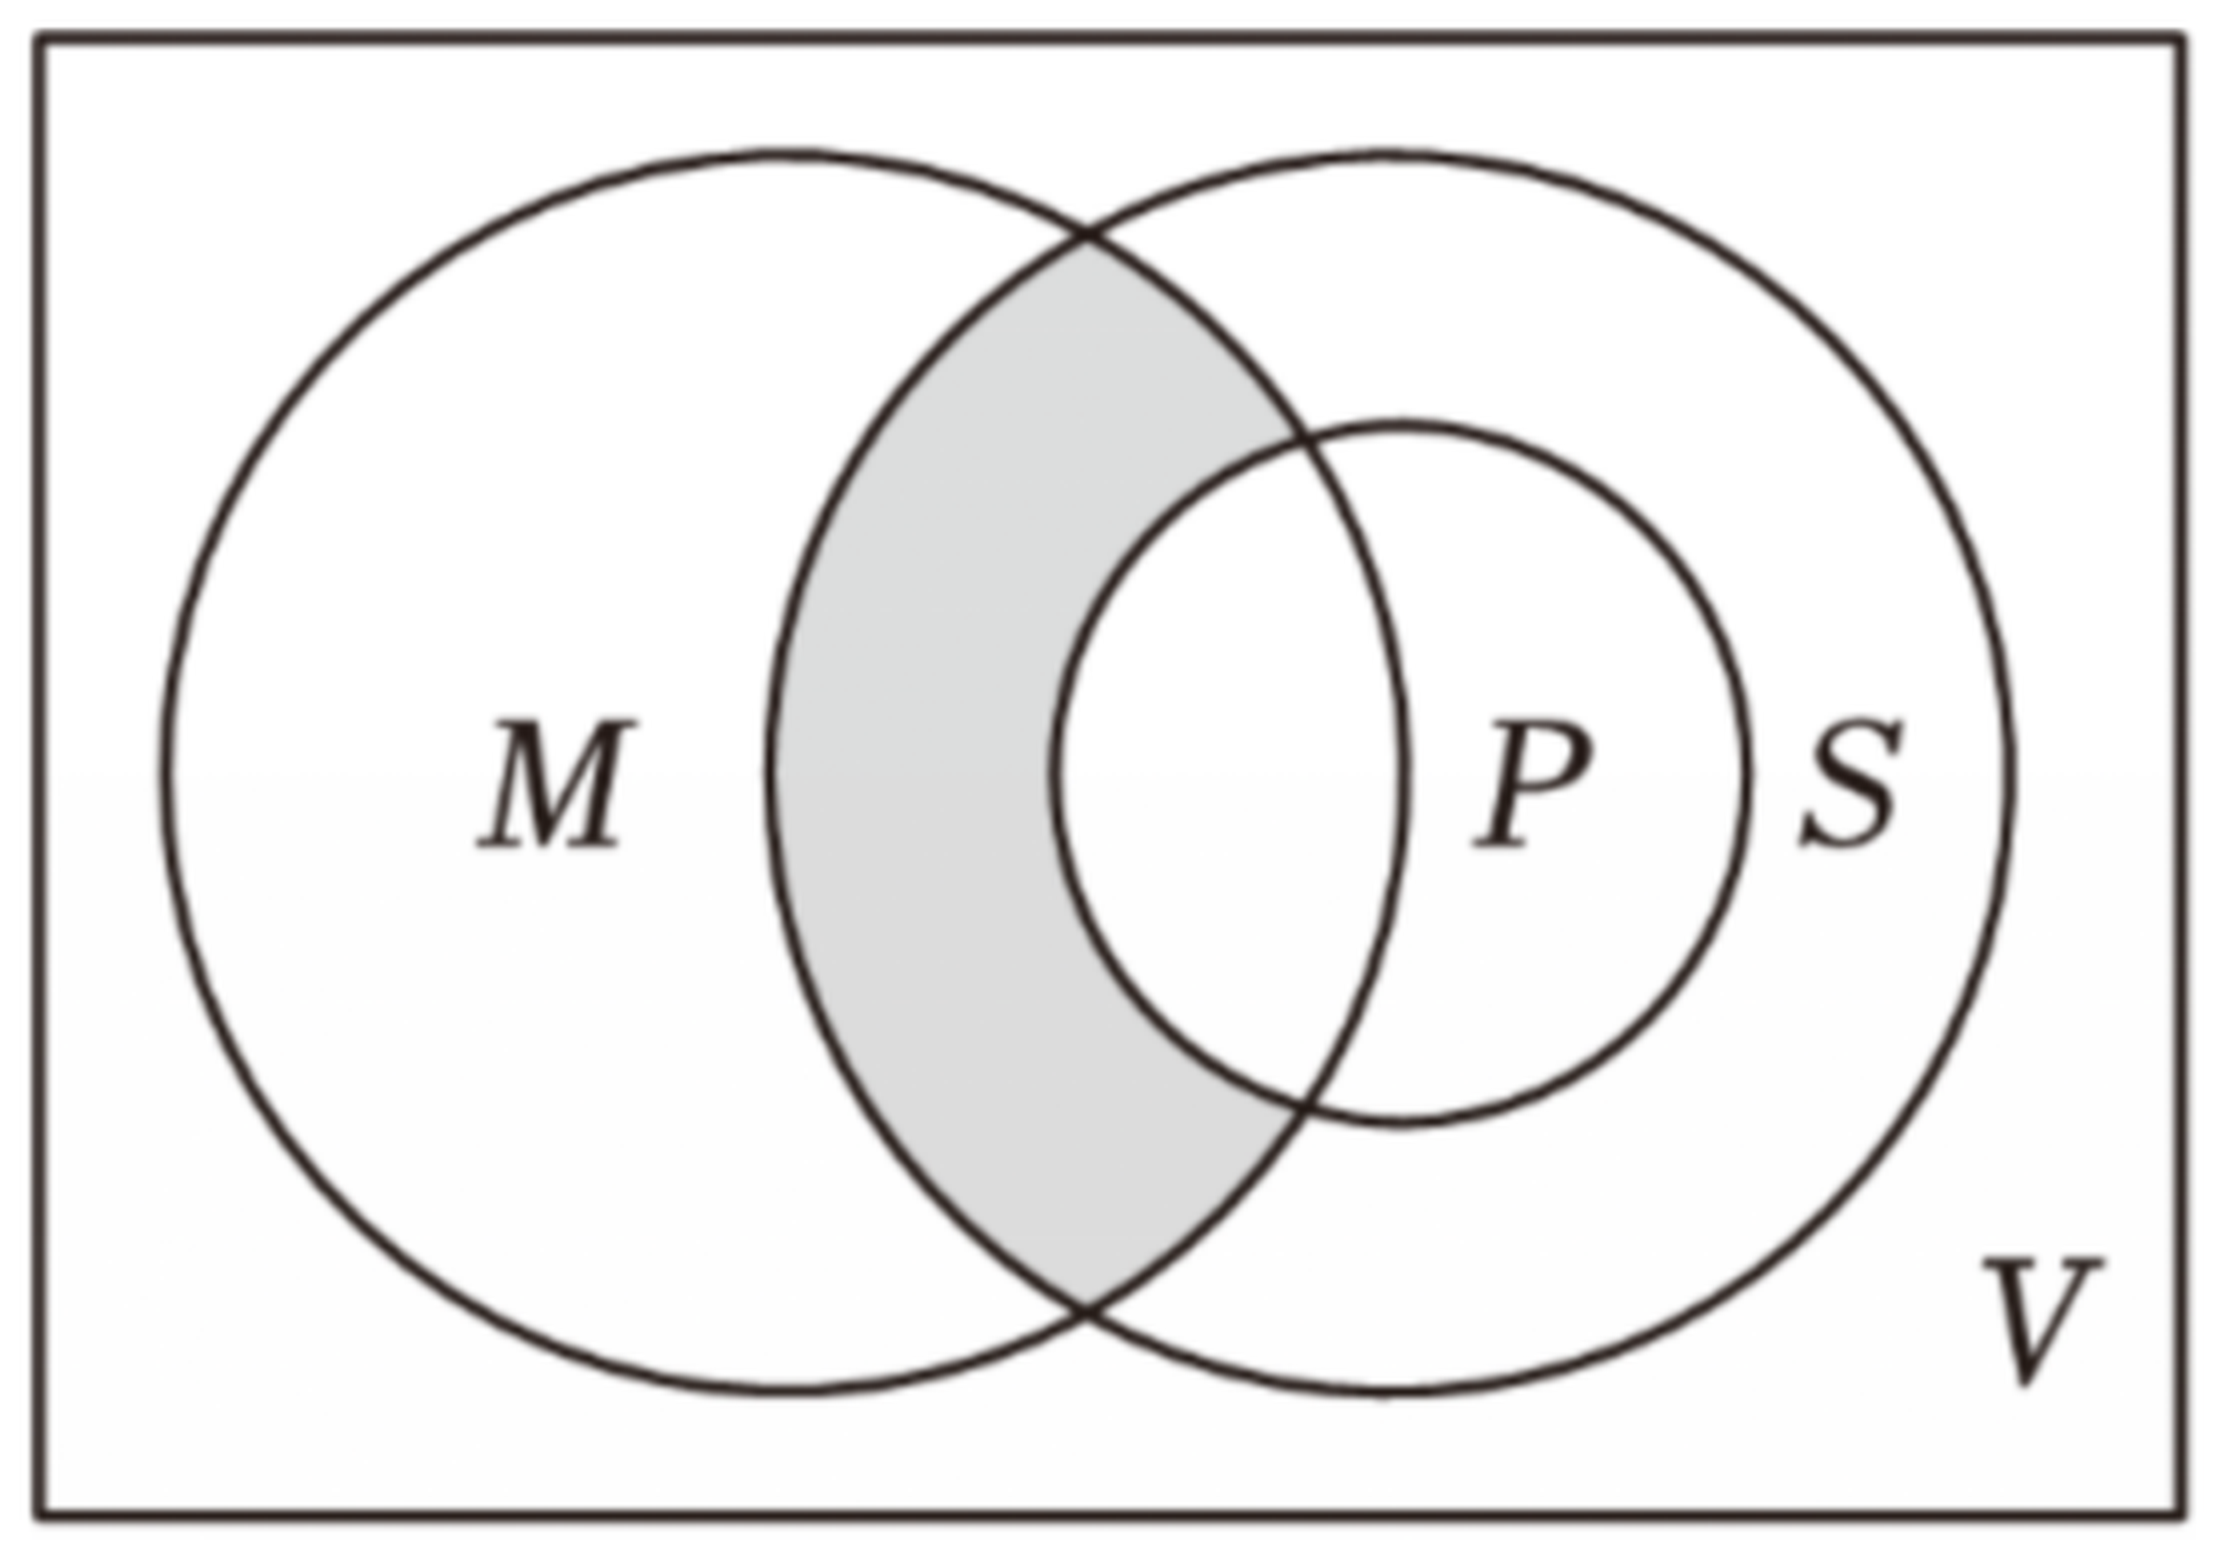
\includegraphics[width=0.38\textwidth]{figures/venn_MPS_V.png}
\end{center}

\ans{$(M\cap S)\cap(\complement_V P)$}

\item 下面六个关系式：① $\varnothing\subseteq\{a\}$；② $a\subseteq\{a\}$；③ $\{a\}\subseteq\{a\}$；④ $\{a\}\in\{a,b\}$；⑤ $a\in\{a,b,c\}$；⑥ $\varnothing\in\{a,b\}$；其中正确的是 \blankline[3.4em].

\ans{①③⑤}

\item 已知集合 $A=\{x\mid -1\le x\le a\}\ne\varnothing$，若 $\{y\mid y=x+1,x\in A\}=\{y\mid y=x^2,x\in A\}$，则实数 $a$ 值为 \blankline[4.4em].

\ans{$0$ 或 $\dfrac{1+\sqrt5}{2}$}

\ifanswer
\solbegin
\step{因为 $A=\{x\mid -1\le x\le a\}\ne\varnothing$，}
\step{所以 $\{y\mid y=x+1,x\in A\}=\{y\mid 0\le y\le a+1\}$，}
\step{$-1\le a\le1$ 时，$\{y\mid y=x^2,x\in A\}=\{y\mid 0\le y\le1\}$，}
\step{$a>1$ 时，$\{y\mid y=x^2,x\in A\}=\{y\mid 0\le y\le a^2\}$，}
\step{① $-1\le a\le1$ 时，$\{y\mid 0\le y\le a+1\}=\{y\mid 0\le y\le1\}$，则 $a+1=1$，解得 $a=0$；}
\step{② $a>1$ 时，$\{y\mid 0\le y\le a+1\}=\{y\mid 0\le y\le a^2\}$，则 $a^2=a+1$，解得 $a=\dfrac{1+\sqrt5}{2}$；}
\step{所以 $a=0$ 或 $\dfrac{1+\sqrt5}{2}$.}
\solend
\fi

\item 设集合 $A=\{(x,y)\mid x+y=22,x>0,y>0,x,y\text{ 均为质数}\}$ 的子集的个数为 \blankline[4.4em].

\ans{$32$}

\ifanswer
\solbegin
\step{集合 $A=\{(x,y)\mid x+y=22,x>0,y>0,x,y\text{ 均为质数}\}$}
\step{$=\{(3,19),(19,3),(5,17),(17,5),(11,11)\}$，则 $A$ 的子集的个数为 $2^5=32$.}
\solend
\fi

% 注：原卷本题题干印作「已知一个有四个数字元素的集合 $S$」；「数字元素」疑为「元素」之衍，
%     但原卷字形确为「数字」二字（已 3× 放大核对过），本稿照录，不代为改写。
\item 已知一个有四个数字元素的集合 $S$，$S$ 的所有子集的元素和（空集的元素和认为是 $0$）的总和为 $16192$，则 $S$ 的元素之和等于 \blankline[4.4em].

\ans{$2024$}

\ifanswer
\solbegin
\step{设 $S=\{a_1,a_2,a_3,a_4\}$，$S$ 的每个元素在所有子集中均出现 $2^3$ 次，}
\step{故 $(a_1+a_2+a_3+a_4)\cdot 2^3=16192$，所以 $a_1+a_2+a_3+a_4=2024$，}
\step{故 $S$ 的元素之和等于 $2024$.}
\solend
\fi

\item 设 $A$ 是非空数集，若对任意 $x$、$y\in A$，都有 $x+y\in A$、$xy\in A$，则称 $A$ 具有性质 $P$，给出以下命题：

①若 $A$ 具有性质 $P$，则 $A$ 可以是有限集；

②若 $A$ 具有性质 $P$，且 $A\ne\R$，则 $\overline A$ 具有性质 $P$；

③若 $A_1$、$A_2$ 具有性质 $P$，且 $A_1\cap A_2\ne\varnothing$，则 $A_1\cap A_2$ 具有性质 $P$；

④若 $A_1$、$A_2$ 具有性质 $P$，则 $A_1\cap A_2$ 具有性质 $P$.

其中所有真命题的序号是 \blankline[4.4em].

\ans{①③}

\ifanswer
\solbegin
\step{对于①，取集合 $A=\{0,1\}$ 具有性质 $P$，故 $A$ 可以是有限集，故①正确；}
\step{对于③，取 $x$、$y\in A_1\cap A_2$，则 $x\in A_1$，$x\in A_2$，$y\in A_1$，$y\in A_2$，}
\step{又 $A_1$、$A_2$ 具有性质 $P$，所以 $x+y\in A_1$，$xy\in A_1$，$x+y\in A_2$，$xy\in A_2$，}
\step{所以 $x+y\in A_1\cap A_2$，$xy\in A_1\cap A_2$，所以 $A_1\cap A_2$ 具有性质 $P$，故③正确；}
\step{对于④，取 $A_1=\{x\mid x=2k,k\in\Z\}$，$A_2=\{x\mid x=3k,k\in\Z\}$，$2\in A_1$，$3\in A_2$，}
\step{但 $2+3\notin A_1\cup A_2$，故④错误；}
\step{对于②，若 $A$ 具有性质 $P$，且 $A\ne\R$，假设 $\overline A$ 也具有性质 $P$，}
\step{设 $0\in A$，在 $\overline A$ 中任取一个 $x$，$x\ne0$，此时可证得 $-x\in A$，}
\step{否则若 $-x\in\overline A$，由于 $\overline A$ 也具有性质 $P$，则 $x+(-x)=0\in\overline A$，}
\step{与 $0\in A$ 矛盾，故 $-x\in A$，}
\step{由于 $A$ 具有性质 $P$，$\overline A$ 也具有性质 $P$，所以 $(-x)^2\in A$，$x^2\in\overline A$，}
\step{而 $(-x)^2=x^2$，这与 $A\cap\overline A=\varnothing$ 矛盾，}
\step{故当 $0\in A$ 且 $A$ 具有性质 $P$ 时，则 $\overline A$ 不具有性质 $P$，}
\step{同理当 $0\in\overline A$ 时，也可以类似推出矛盾，故②错误.}
\step{故正确的是①③.}
\solend
\fi

\item 已知 $S=\{1,2,3,4,5\}$，$A=\{1,2,5\}$，$T=\{t_1,t_2\}\subseteq S$，记 $A_1=\{x\mid x=a+t_1,a\in A,t_1\in T\}$，$A_2=\{x\mid x=b+t_2,b\in A,t_2\in T\}$，若 $A_1\cap A_2=\varnothing$，则集合 $T$ 为 \blankline[5.4em].

\ans{$T=\{1,3\}$ 或 $T=\{2,4\}$ 或 $T=\{3,5\}$}

\ifanswer
\solbegin
\step{若 $A_1\cap A_2=\varnothing$，即 $a+t_1\ne b+t_2$，则 $t_1-t_2\ne a-b$，其中 $a$、$b\in A$，}
\step{否则 $t_1+a=t_2+b$，$A_1\cap A_2\ne\varnothing$，}
\step{又 $S=\{1,2,3,4,5\}$，$A=\{1,2,5\}$，$T=\{t_1,t_2\}\subseteq S$，}
\step{$2-1=1$，$5-2=3$，$5-1=4$，则 $t_1$、$t_2$ 相差 $2$，}
\step{所以 $T=\{1,3\}$ 或 $T=\{2,4\}$ 或 $T=\{3,5\}$.}
\solend
\fi

\end{enumerate}

\bigsec{二、解答题}

\begin{enumerate}
\setcounter{enumi}{13}

\item 设集合 $P=\{1,2,3,m\}$，$Q=\{3,m^2\}$，且 $\overline P\cap Q=\varnothing$，求实数 $m$ 的值组成的集合.

\ans{$\{-1,0,\pm\sqrt2\}$}

\ansspace[5]

\ifanswer
\solbegin
\step{因为 $\overline P\cap Q=\varnothing$，所以 $Q\subseteq P$，所以 $m^2=1$ 或 $m^2=2$ 或 $m^2=m$，}
\step{考虑互异性，得 $m=-1$ 或 $m=\pm\sqrt2$ 或 $m=0$，}
\step{所以实数 $m$ 的值组成的集合为 $\{-1,0,\pm\sqrt2\}$.}
\solend
\fi

\item 若集合 $A=(-\infty,2]$，$B=\{x\mid kx+1<0,k\in\R\}$，$A\cap B=\varnothing$，求实数 $k$ 的取值范围.

\ans{$\left[-\dfrac12,0\right]$}

\ansspace[5]

\ifanswer
\solbegin
\step{若 $B=\varnothing$，则 $k=0$，符合题意，}
\step{若 $B\ne\varnothing$，当 $k>0$ 时，$B=\left(-\infty,-\dfrac1k\right)$，$A\cap B\ne\varnothing$，不合题意；}
\step{当 $k<0$ 时，$B=\left(-\dfrac1k,+\infty\right)$，由 $A\cap B=\varnothing$ 得 $-\dfrac1k\ge2$，即 $-\dfrac12\le k<0$，}
\step{故 $k$ 的取值范围是 $\left[-\dfrac12,0\right]$.}
\solend
\fi

\item 已知集合 $A=\{-4,2a-1,a^2\}$，$B=\{a-5,1-a,9\}$，分别求适合下列条件的 $a$ 的值.

% 两个小问不许与题干分家：试卷版第 2 页页末原本正好把 (1) 留在页底、(2) 翻到次页，
% 与 2026-09-15 修的三类难看切页同源，故在这里也加 \keepwithprev 守卫（三版都生效）。
\keepwithprev
（1）$9\in(A\cap B)$；

\keepwithprev
（2）$\{9\}=A\cap B$.

\ans{（1）$a=5$ 或 $a=-3$；（2）$a=-3$}

\ansspace[5]

\ifanswer
\solbegin
\stepm{（1）}{$9\in(A\cap B)$，所以 $9\in A$，}
\step{当 $2a-1=9$ 时，$a=5$，当 $a^2=9$ 时，即 $a=\pm3$，}
% 注：原卷此句结论印作「所以 $a$ 的值为 $5\backslash-3$」——「\」应是顿号之误，
%     本稿照录原卷字形（见文件头「原卷存疑」②）；按文意即 $a=5$ 或 $a=-3$。
\step{当 $a=3$ 时，$a-5=1-a$ 舍去，所以 $a$ 的值为 $5\backslash-3$.}
\stepm{（2）}{结合（1）的结论：}
\step{当 $2a-1=9$ 即 $a=5$ 时，$1-a=-4$，$\{9\}\ne(A\cap B)$，}
\step{当 $a^2=9$ 时，即 $a=\pm3$，当 $a=3$ 时，$a-5=1-a$ 舍去，}
\step{所以 $a$ 的值为 $-3$.}
\solend
\fi

\item 已知集合 $M=\{a,ab,a-b\}$，$N=\{0,|a|,b\}$，且 $M=N$，求实数 $a$、$b$ 的值.

\ans{$a=b=-1$}

\ansspace[5]

\ifanswer
\solbegin
\step{由集合元素的互异性，得 $a\ne0$，且 $b\ne0$，所以 $a-b=0$，即 $a=b$，}
\step{所以 $ab=|a|$，又由 $|a|\ne b=a$，得 $a<0$，故 $a=b=-1$.}
\solend
\fi

\item 已知集合 $A=\{x\mid -2<x<7\}$，$B=\{x\mid m+1\le x\le 2m-1\}$.

\keepwithprev
（1）当 $m=4$ 时，求 $A\cap B$、$A\cup B$；

\keepwithprev
（2）若 $A\cap B=B$，求实数 $m$ 的取值范围.

\ans{（1）$A\cap B=[5,7)$，$A\cup B=(-2,7]$；（2）$(-\infty,4)$}

\ansspace[5]

\ifanswer
\solbegin
\stepm{（1）}{当 $m=4$ 时，得集合 $A=\{x\mid -2<x<7\}$，$B=\{x\mid 5\le x\le7\}$，}
\step{得 $A\cap B=[5,7)$，$A\cup B=(-2,7]$.}
\stepm{（2）}{由 $A\cap B=B$ 得 $B\subseteq A$，}
\step{①当 $B=\varnothing$ 时，得 $m+1>2m-1$，解得 $m<2$；}
\step{②当 $B\ne\varnothing$ 时，得 $\begin{cases}m+1>-2\\ 2m-1<7\\ m+1\le2m-1\end{cases}$，解得 $2\le m<4$；}
\step{综上，实数 $m$ 的取值范围是 $(-\infty,4)$.}
\solend
\fi

\item 若集合 $A=\{x\mid x^2+5x-6=0\}$，$B=\{x\mid x^2+2(m+1)x+m^2-3=0\}$.

\keepwithprev
（1）当 $m=0$ 时，求集合 $A\cup B$；

\keepwithprev
（2）若 $A\cap B=B$，求实数 $m$ 的取值范围.

\ans{（1）$A\cup B=\{1,-6,-3\}$；（2）$\{m\mid m\le-2\}$}

\ansspace[5]

\ifanswer
\solbegin
\stepm{（1）}{由题意得，集合 $A=\{x\mid x^2+5x-6=0\}=\{1,-6\}$，}
\step{当 $m=0$ 时，$B=\{x\mid x^2+2x-3=0\}=\{1,-3\}$，}
\step{所以 $A\cup B=\{1,-6,-3\}$；}
\stepm{（2）}{由（1）得集合 $A=\{1,-6\}$，$B=\{x\mid x^2+2(m+1)x+m^2-3=0\}$，}
\step{若 $A\cap B=B$ 得 $B\subseteq A$，所以 $B=\varnothing$ 或 $\{-6\}$ 或 $\{1\}$ 或 $\{1,-6\}$，}
\step{当 $B=\varnothing$ 时，$\Delta=4(m+1)^2-4(m^2-3)<0$，解得 $m<-2$，}
\step{当 $B=\{-6\}$ 时，则 $\begin{cases}\Delta=4(m+1)^2-4(m^2-3)=0\\ 36-12(m+1)+m^2-3=0\end{cases}$，无解，}
\step{当 $B=\{1\}$ 时，则 $\begin{cases}\Delta=4(m+1)^2-4(m^2-3)=0\\ 1+2(m+1)+m^2-3=0\end{cases}$，解得 $m=-2$，}
\step{当 $B=\{1,-6\}$ 时，则 $\begin{cases}\Delta=4(m+1)^2-4(m^2-3)>0\\ 1+(-6)=-2(m+1)\\ 1\times(-6)=m^2-3\end{cases}$，无解，}
\step{综上所述，实数 $m$ 的取值范围为 $\{m\mid m\le-2\}$.}
\solend
\fi

% 压轴题：其后已无内容，故作答区全用可丢弃胶水（\ansspace*），并在题目前先量一下版面。
\ansneed{8cm}
\item 对于点集 $A=\{(x,y)\mid x=m,y=-3x+2,m\in\N,m\ge1\}$，$B=\{(x,y)\mid x=n,y=a(x^2-x+1),n\in\N,n\ge1\}$，是否存在非零整数 $a$，使得 $A\cap B\ne\varnothing$？

\ans{$a=-1$}

\ansspace*[10]

\ifanswer
\solbegin
\step{当 $A\cap B\ne\varnothing$ 时，$-3x+2=a(x^2-x+1)$，}
\step{$ax^2+(3-a)x+a-2=0$ ①有正整数解，}
\step{所以 $\Delta=(3-a)^2-4a(a-2)=-3a^2+2a+9$ 是平方数，}
\step{所以 $3a^2-2a-9\le0$，$\dfrac{1-2\sqrt7}{3}\le a\le\dfrac{1+2\sqrt7}{3}$，$a\ne0$，$a\in\Z$，}
\step{所以 $a=\pm1$ 或 $a=2$，}
\step{$a=-1$ 时 $\Delta=4$，这时①变为 $-x^2+4x-3=0$，解得 $x_1=1$，$x_2=3$，}
\step{$A\cap B=\{(1,-1),(3,-7)\}$.}
\step{$a=1$ 时 $\Delta=8$，不是平方数.}
\step{$a=2$ 时 $\Delta=1$，这时①变为 $2x^2+x=0$，没有正整数解.}
\step{所以 $a=-1$.}
\solend
\fi

\end{enumerate}

\end{document}
"
%
% 原始材料是微信公众号图文（公众号「魔都数学加油站」，作者署名「破晓」，
% 原文链接 https://mp.weixin.qq.com/s/tHqWSV1StO5SHSXXQ4jeUA），正文为 6 张 PNG 页；
% 原文本身就是一份**讲评版**——题目下方直接印出【答案】或【解析】。本稿把答案与解析
% 移到答案版，试卷版即一张干净的空卷；试题文字、答案与解析均照原卷录入。
%
% 与原卷的排版差异（均已在 README「说明」中交代）：
%   ① 原文自**第 3 题**起（第 1、2 题未在该文发布），源码里以 \setcounter{enumi}{2} 起编；
%      全卷只有「一、填空题」「二、解答题」两节，无选择题；
%   ② 原卷本就印有两个分节标题（已在原图上逐页放大核对过），本稿照原卷分节，只把标题改排
%      成全稿统一的「大节标题」样式；
%   ③ 原卷的实数集、整数集、自然数集符号作正体 $R$、$Z$、$N$（第 15 题作粗体 $\mathbf{R}$，
%      第 20 题有 $N$ 与斜体 $Z$），本稿按全稿惯例统一写作 $\R$、$\Z$、$\N$；
%   ④ 第 4 题的韦恩图在原卷里印在【解析】右侧（题干并无「如图」二字），故本稿把该图放进
%      答案版的解析块内（`figures/venn_AB_survey_50_x.png`）；第 6、7 题的韦恩图是**题干图**
%      （题干作「图中阴影部分所表示的集合」），两版都排（`figures/venn_A_shaded_U.png`、
%      `figures/venn_MPS_V.png`）。三张图都取自原卷截图、4× LANCZOS 放大，不用 TikZ 手绘；
%   ⑤ 本卷也是「讲评版」，解析按全稿统一的 \solbegin/\step 分步重排（原卷为连续段落），
%      分步不改一字，只断句、断行；
%   ⑥ 标题前缀照**原卷**作「2026--2027 年…」（原卷标题即作「2026-2027年延安中学高一上周末
%      作业 2」）。同校的 高一06 作「学年度」——那是 高一02—高一09 那一批入库时统一改的；
%      后续入库的卷（高一10—高一17 与本卷）一律照原卷保留「年」，未强改，故同校两卷前缀不同。
%
% 原卷存疑两处（已逐处放大到能看清字形后核对，本稿照录并加注，见各题下的 `%` 注）：
%   （另有第三处「第 12 题【解析】末句」原先记作存疑，2026-09-26 第二轮核对放大后发现
%     原卷印的是「$0\in\overline A$」——A 上确有横杠，是本稿当初漏抄了 $\overline{}$；
%     已按原卷补回，故该条从存疑清单里删去，不计为原卷问题。）
%   ① 第 11 题题干印作「已知一个有四个数字元素的集合 $S$」，「数字元素」疑为「元素」之衍；
%   ② 第 16 题 (1) 结论印作「$a$ 的值为 $5\backslash-3$」，其中的「\」应是顿号之误
%      （由 (2) 的结论「$a$ 的值为 $-3$」可反推，(1) 的答案是 $5$ 或 $-3$）；

% 本篇在公众号「魔都数学加油站」连载里的编号是「27学年高一19」，本地编号与之对齐（高一19）；
% 对应关系见 README「与公众号连载号的对照表」。
\documentclass[a4paper,11pt]{article}
\usepackage{common}

\begin{document}

\examtitlest{2026--2027 年延安中学高一上周末作业 2}{集合与常用逻辑用语}

\bigsec{一、填空题}

\begin{enumerate}
% 原卷填空题从第 3 题起（1、2 未在该文中发布），须与解答题的 \setcounter{enumi}{13} 对齐
\setcounter{enumi}{2}
\item 已知全集 $U=\{1,2,3,4,5\}$，$M=\{1,2\}$，$P=\{1,3,5\}$，则 $M\cap\overline P=$ \blankline[4.4em].

\ans{$\{2\}$}

\item 某公司共有 $50$ 人，此次组织参加社会公益活动，其中参加 $A$ 项公益活动的有 $28$ 人，参加 $B$ 项公益活动的有 $33$ 人，且 $A$、$B$ 两项公益活动都不参加的人数比都参加的人数的三分之一多 $1$ 人，则只参加 $A$ 项不参加 $B$ 项的人数是 \blankline[4.4em].

\ans{$10$}

\ifanswer
\solbegin
\step{如图所示，设 $A$、$B$ 两项公益活动都参加的有 $x$ 人，}
\begin{center}
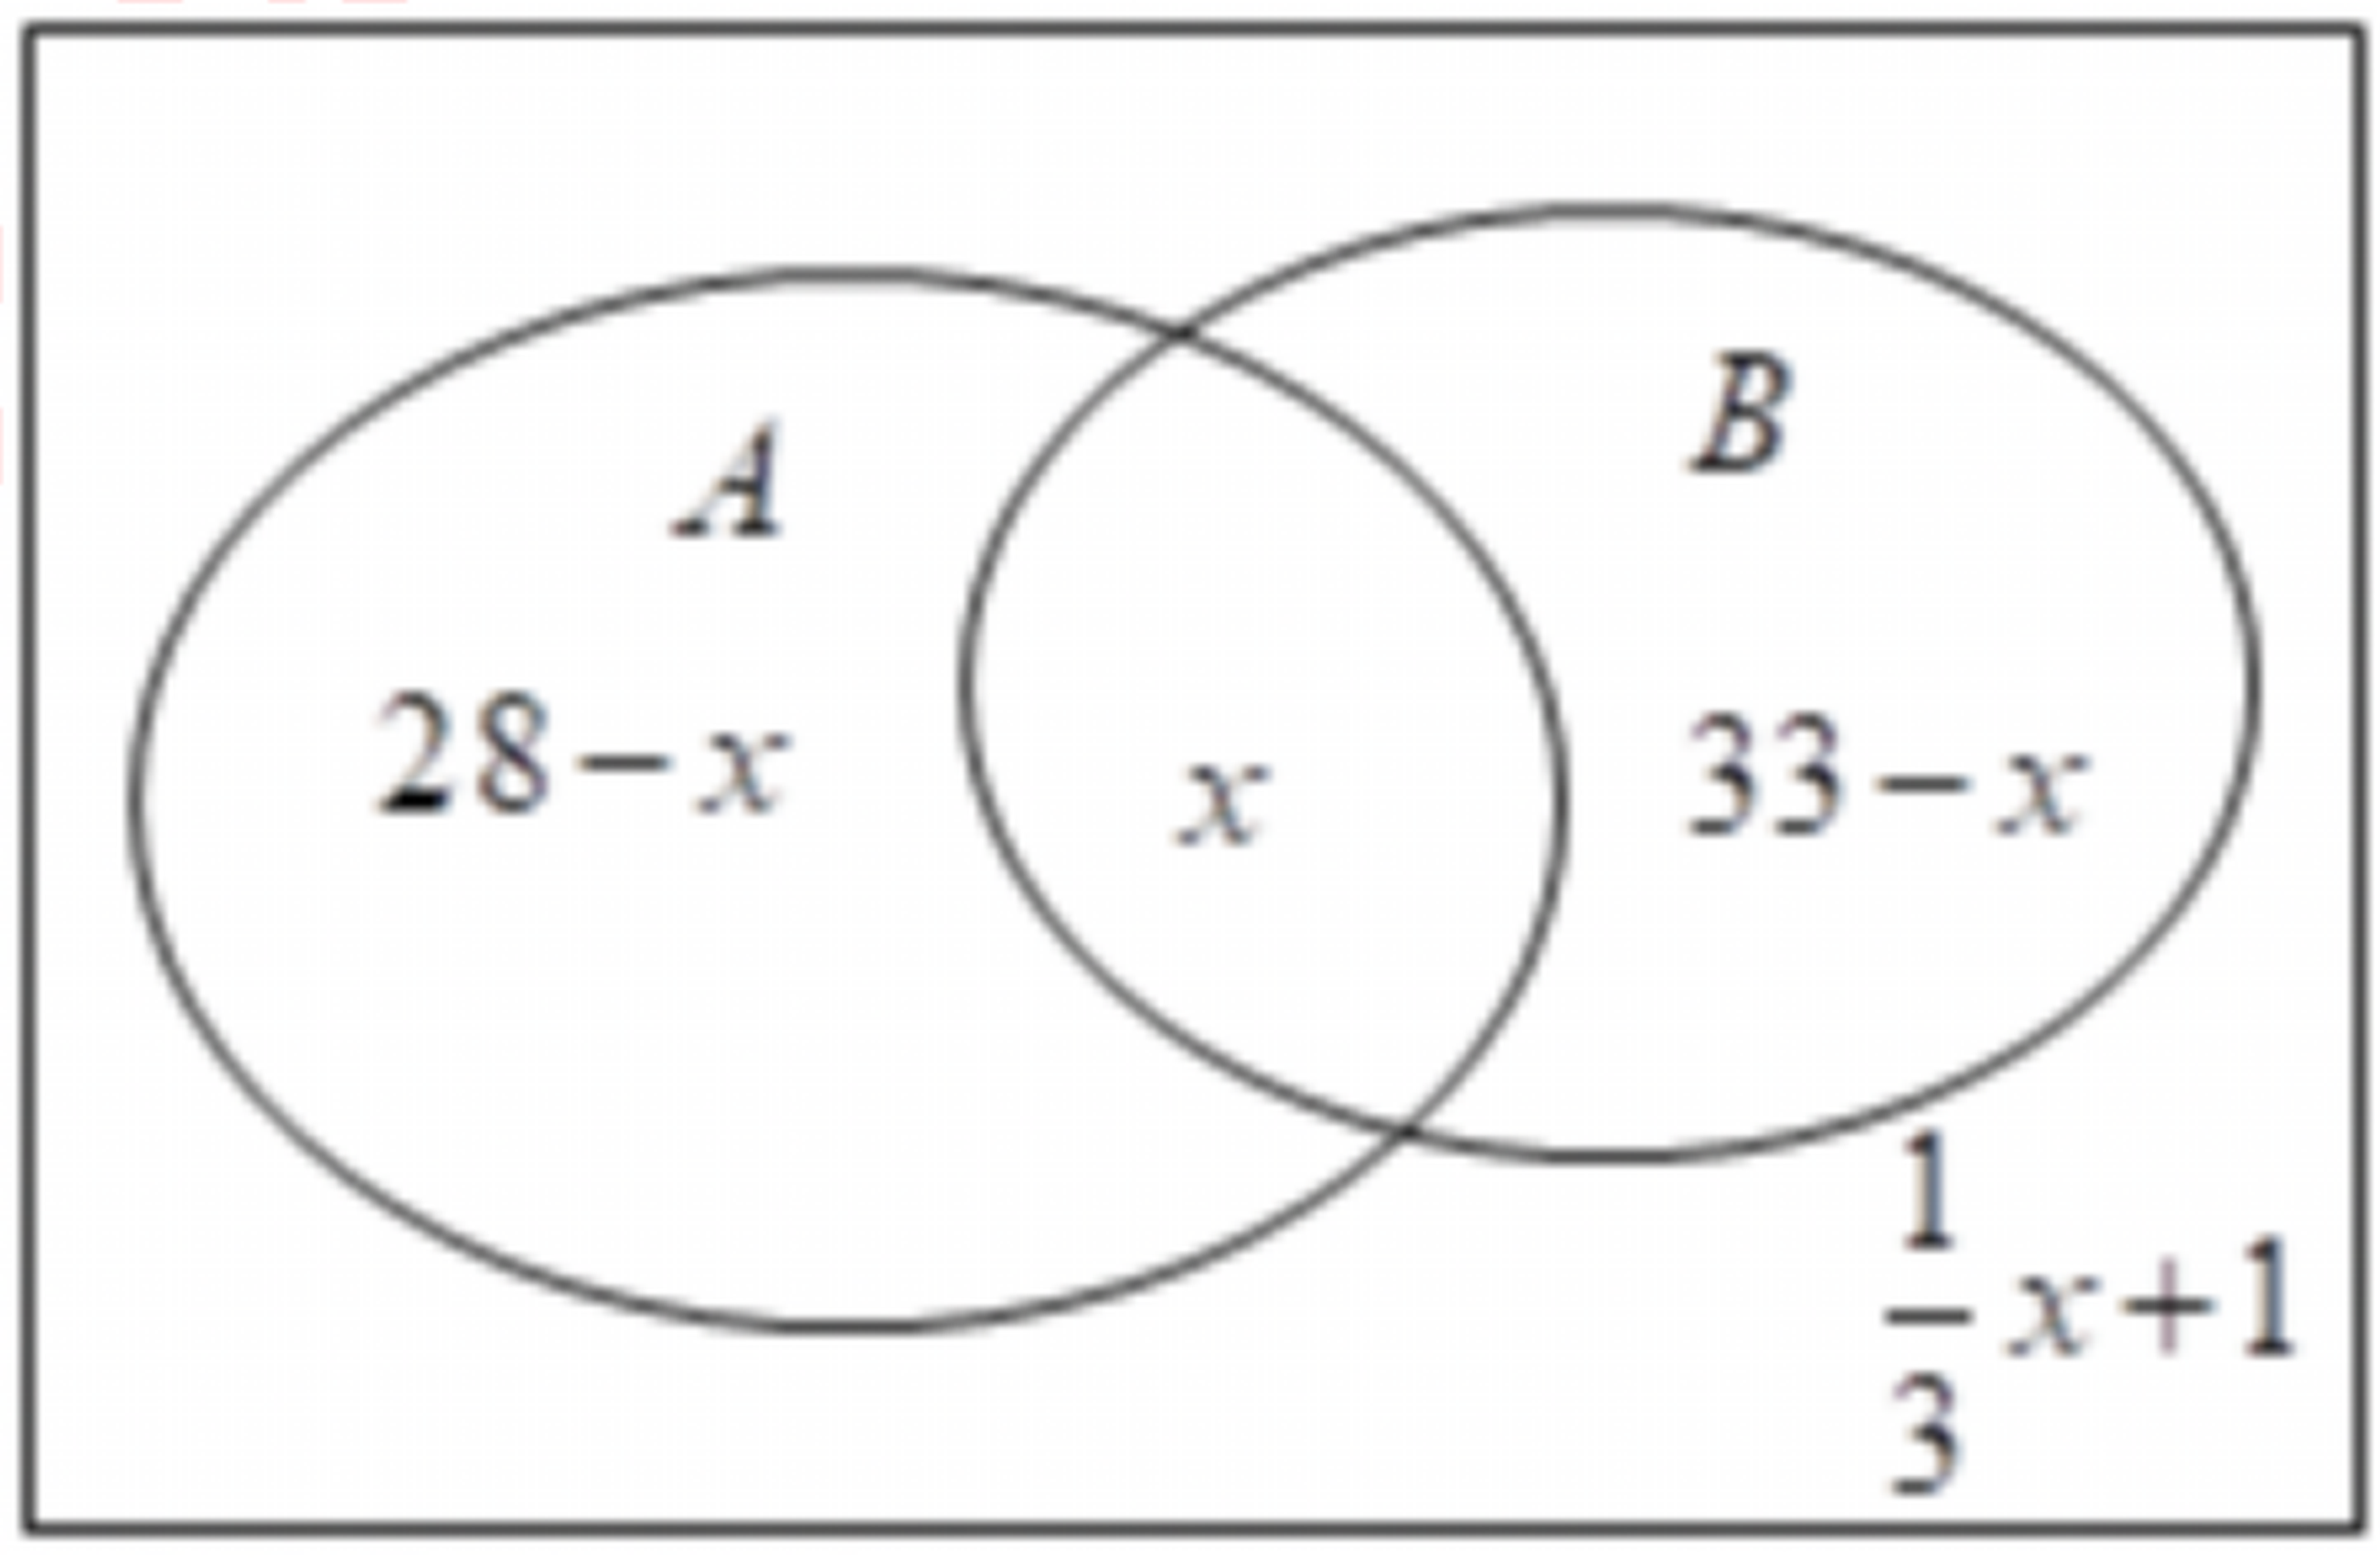
\includegraphics[width=0.42\textwidth]{figures/venn_AB_survey_50_x.png}
\end{center}
\step{则仅参加 $A$ 项的有 $(28-x)$ 人，仅参加 $B$ 项的有 $(33-x)$ 人，}
\step{$A$、$B$ 两项公益活动都不参加的有 $\left(\dfrac13x+1\right)$ 人，}
\step{由题意得 $x+(28-x)+(33-x)+\left(\dfrac13x+1\right)=50$，解得 $x=18$，}
\step{所以只参加 $A$ 项不参加 $B$ 项的有 $28-18=10$ 人.}
\solend
\fi

\item 设集合 $A=\{x\mid x^2-3x+2=0\}$，则满足 $A\cup B=\{0,1,2\}$ 的集合 $B$ 的个数是 \blankline[4.4em].

\ans{$4$}

\ifanswer
\solbegin
\step{$A=\{x\mid x^2-3x+2=0\}=\{x\mid x=1\text{ 或 }x=2\}=\{1,2\}$，}
\step{若 $A\cup B=\{0,1,2\}$，则 $0\in B$，}
\step{则 $B=\{0\},\{0,2\},\{1,0\},\{0,1,2\}$，共 $4$ 个.}
\solend
\fi

\item 已知全集 $U=\R$，集合 $A=\{x\mid x^2<4\}$，$B=\{y\mid y=x^2\}$，则图中阴影部分所表示的集合为 \blankline[4.4em].

\begin{center}
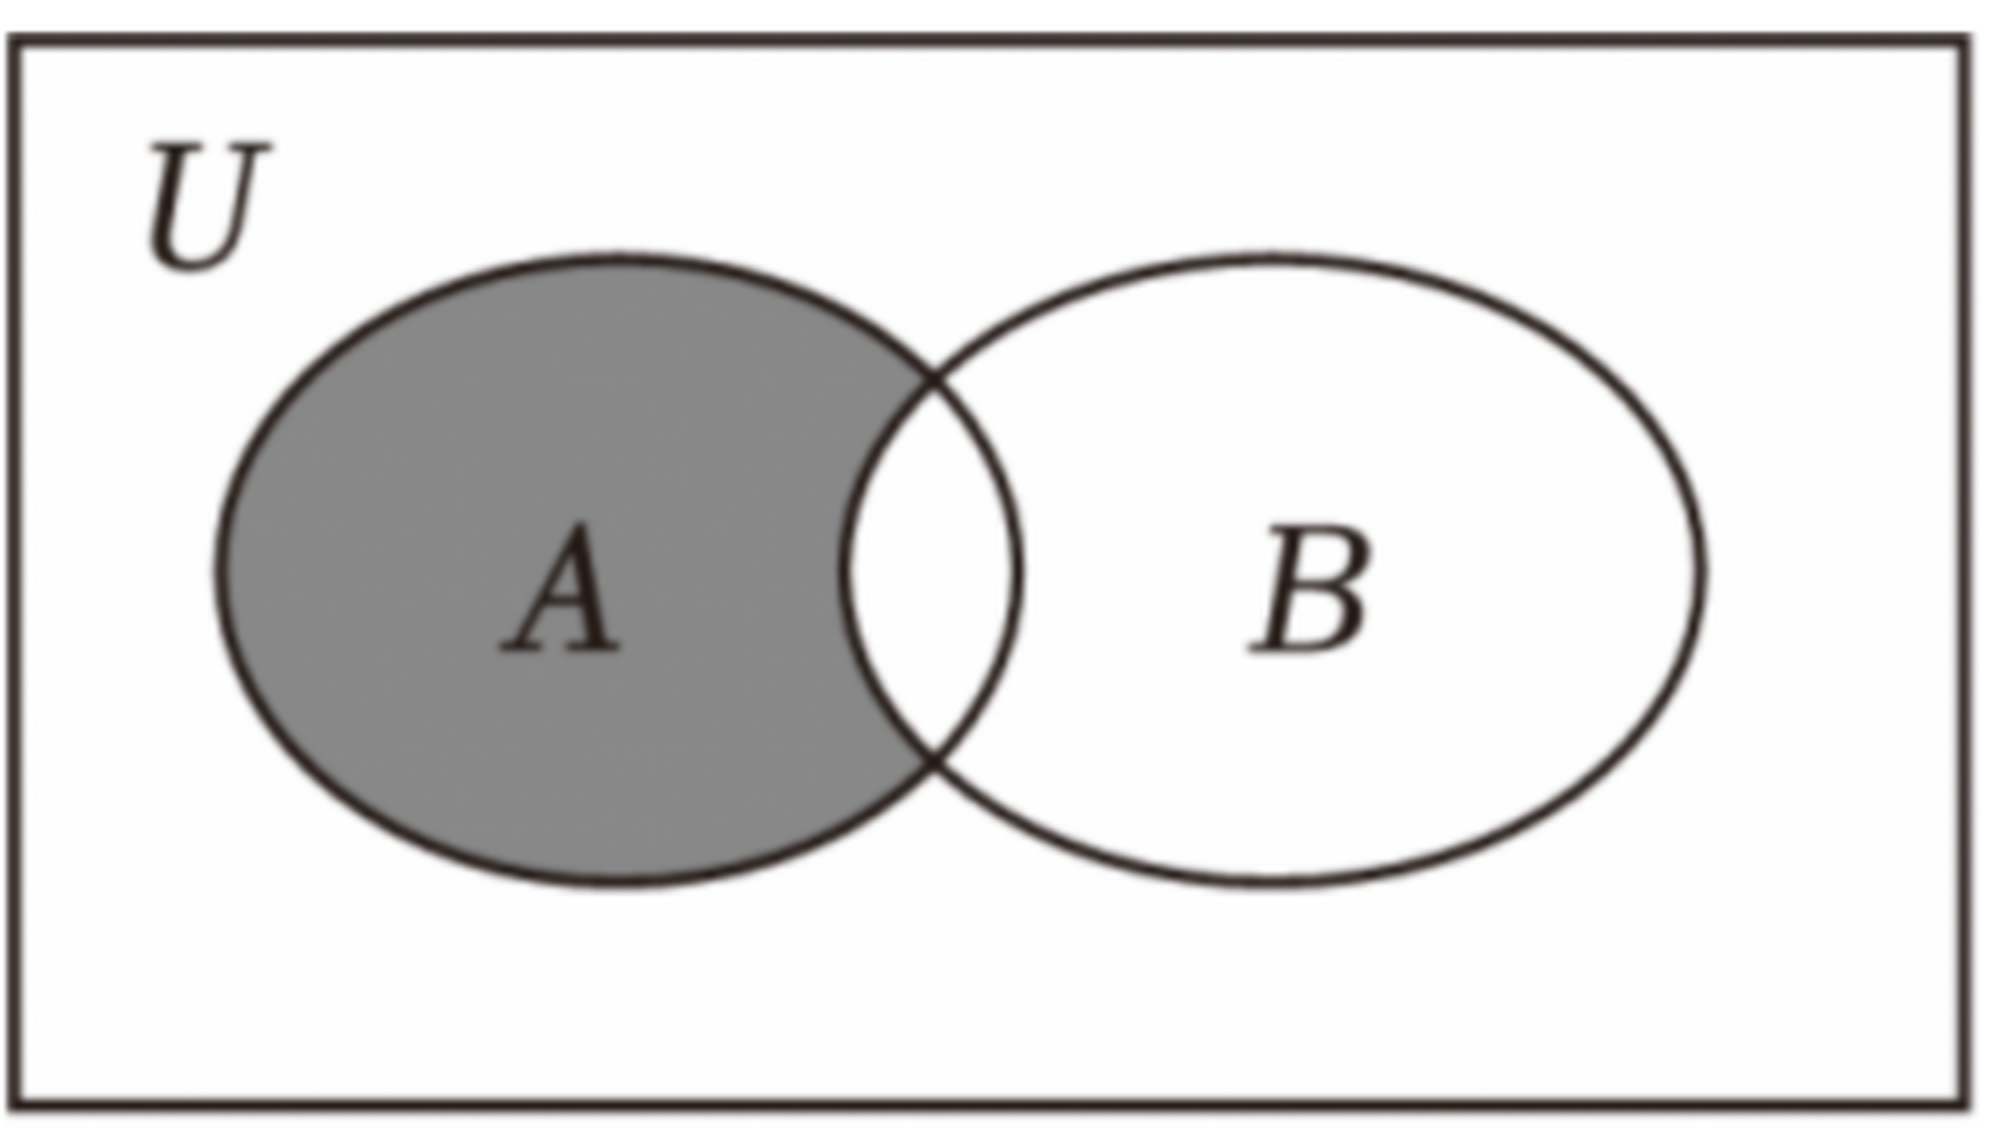
\includegraphics[width=0.34\textwidth]{figures/venn_A_shaded_U.png}
\end{center}

\ans{$A\cap\overline B=(-2,0)$}

\ifanswer
\solbegin
\step{集合 $A=\{x\mid x^2<4\}=(-2,2)$，$B=\{y\mid y=x^2\}=[0,+\infty)$，}
\step{图中阴影部分所表示的集合是 $A\cap\overline B=(-2,0)$.}
\solend
\fi

\item 如图所示，$M$、$P$、$S$ 是 $V$ 的三个子集，则阴影部分所表示的集合是 \blankline[5.4em].

\begin{center}
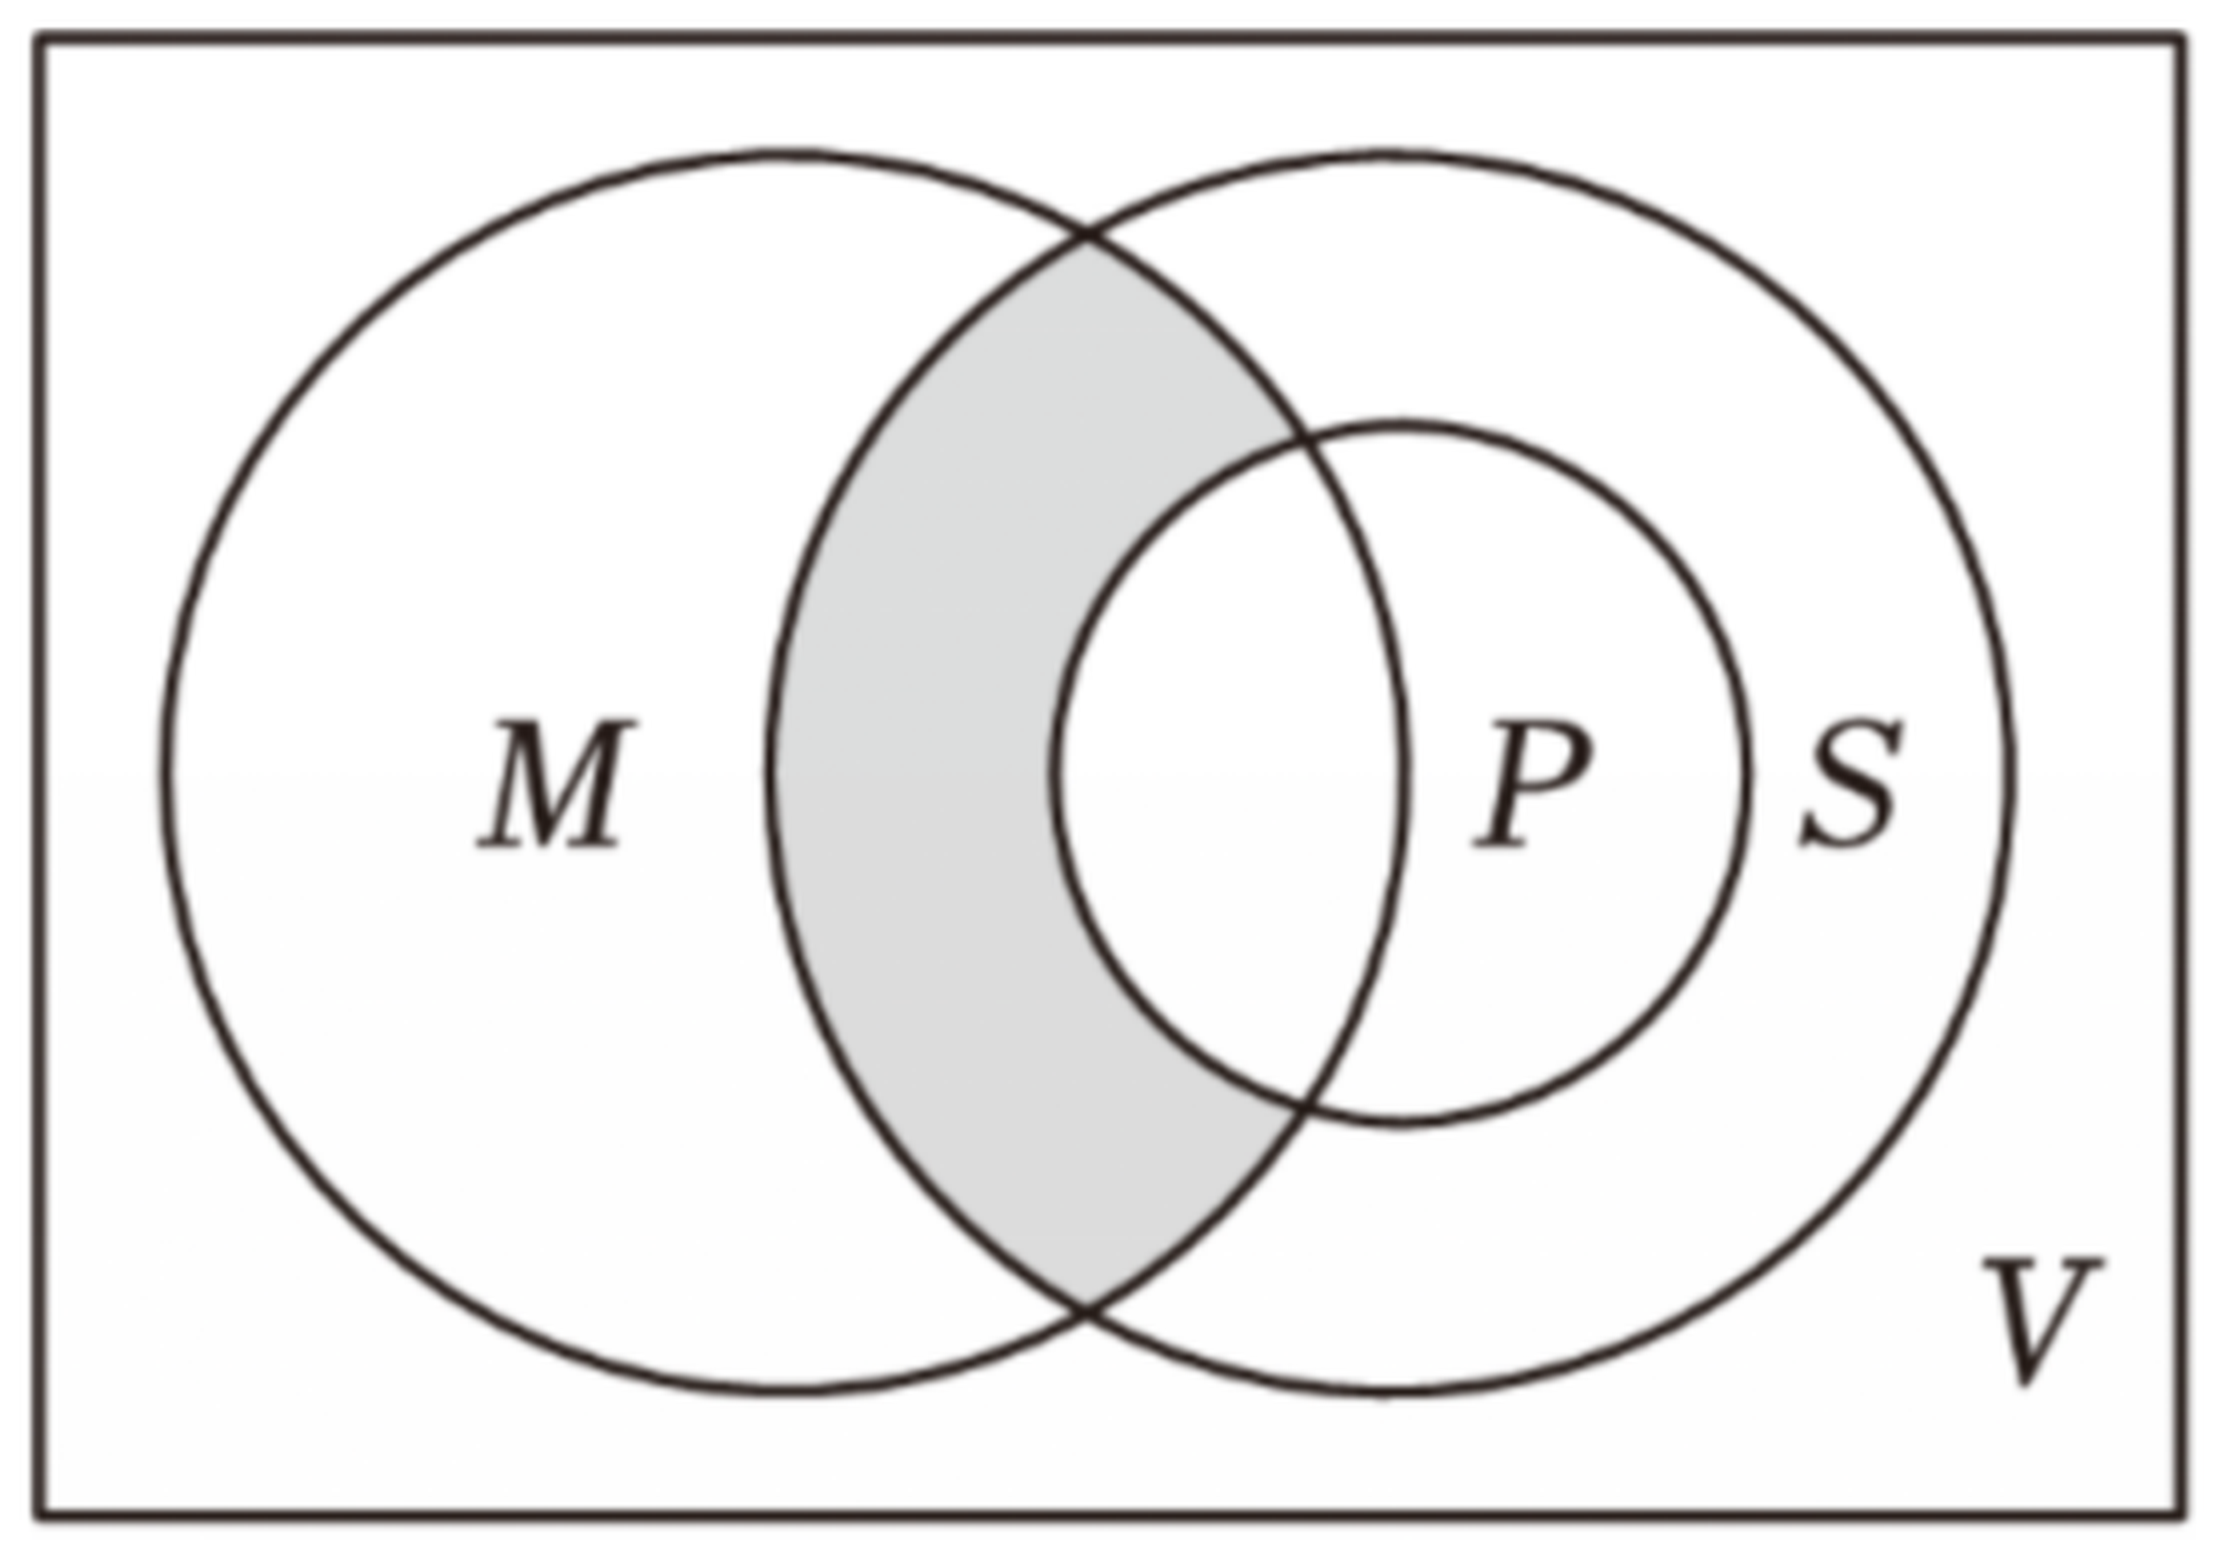
\includegraphics[width=0.38\textwidth]{figures/venn_MPS_V.png}
\end{center}

\ans{$(M\cap S)\cap(\complement_V P)$}

\item 下面六个关系式：① $\varnothing\subseteq\{a\}$；② $a\subseteq\{a\}$；③ $\{a\}\subseteq\{a\}$；④ $\{a\}\in\{a,b\}$；⑤ $a\in\{a,b,c\}$；⑥ $\varnothing\in\{a,b\}$；其中正确的是 \blankline[3.4em].

\ans{①③⑤}

\item 已知集合 $A=\{x\mid -1\le x\le a\}\ne\varnothing$，若 $\{y\mid y=x+1,x\in A\}=\{y\mid y=x^2,x\in A\}$，则实数 $a$ 值为 \blankline[4.4em].

\ans{$0$ 或 $\dfrac{1+\sqrt5}{2}$}

\ifanswer
\solbegin
\step{因为 $A=\{x\mid -1\le x\le a\}\ne\varnothing$，}
\step{所以 $\{y\mid y=x+1,x\in A\}=\{y\mid 0\le y\le a+1\}$，}
\step{$-1\le a\le1$ 时，$\{y\mid y=x^2,x\in A\}=\{y\mid 0\le y\le1\}$，}
\step{$a>1$ 时，$\{y\mid y=x^2,x\in A\}=\{y\mid 0\le y\le a^2\}$，}
\step{① $-1\le a\le1$ 时，$\{y\mid 0\le y\le a+1\}=\{y\mid 0\le y\le1\}$，则 $a+1=1$，解得 $a=0$；}
\step{② $a>1$ 时，$\{y\mid 0\le y\le a+1\}=\{y\mid 0\le y\le a^2\}$，则 $a^2=a+1$，解得 $a=\dfrac{1+\sqrt5}{2}$；}
\step{所以 $a=0$ 或 $\dfrac{1+\sqrt5}{2}$.}
\solend
\fi

\item 设集合 $A=\{(x,y)\mid x+y=22,x>0,y>0,x,y\text{ 均为质数}\}$ 的子集的个数为 \blankline[4.4em].

\ans{$32$}

\ifanswer
\solbegin
\step{集合 $A=\{(x,y)\mid x+y=22,x>0,y>0,x,y\text{ 均为质数}\}$}
\step{$=\{(3,19),(19,3),(5,17),(17,5),(11,11)\}$，则 $A$ 的子集的个数为 $2^5=32$.}
\solend
\fi

% 注：原卷本题题干印作「已知一个有四个数字元素的集合 $S$」；「数字元素」疑为「元素」之衍，
%     但原卷字形确为「数字」二字（已 3× 放大核对过），本稿照录，不代为改写。
\item 已知一个有四个数字元素的集合 $S$，$S$ 的所有子集的元素和（空集的元素和认为是 $0$）的总和为 $16192$，则 $S$ 的元素之和等于 \blankline[4.4em].

\ans{$2024$}

\ifanswer
\solbegin
\step{设 $S=\{a_1,a_2,a_3,a_4\}$，$S$ 的每个元素在所有子集中均出现 $2^3$ 次，}
\step{故 $(a_1+a_2+a_3+a_4)\cdot 2^3=16192$，所以 $a_1+a_2+a_3+a_4=2024$，}
\step{故 $S$ 的元素之和等于 $2024$.}
\solend
\fi

\item 设 $A$ 是非空数集，若对任意 $x$、$y\in A$，都有 $x+y\in A$、$xy\in A$，则称 $A$ 具有性质 $P$，给出以下命题：

①若 $A$ 具有性质 $P$，则 $A$ 可以是有限集；

②若 $A$ 具有性质 $P$，且 $A\ne\R$，则 $\overline A$ 具有性质 $P$；

③若 $A_1$、$A_2$ 具有性质 $P$，且 $A_1\cap A_2\ne\varnothing$，则 $A_1\cap A_2$ 具有性质 $P$；

④若 $A_1$、$A_2$ 具有性质 $P$，则 $A_1\cap A_2$ 具有性质 $P$.

其中所有真命题的序号是 \blankline[4.4em].

\ans{①③}

\ifanswer
\solbegin
\step{对于①，取集合 $A=\{0,1\}$ 具有性质 $P$，故 $A$ 可以是有限集，故①正确；}
\step{对于③，取 $x$、$y\in A_1\cap A_2$，则 $x\in A_1$，$x\in A_2$，$y\in A_1$，$y\in A_2$，}
\step{又 $A_1$、$A_2$ 具有性质 $P$，所以 $x+y\in A_1$，$xy\in A_1$，$x+y\in A_2$，$xy\in A_2$，}
\step{所以 $x+y\in A_1\cap A_2$，$xy\in A_1\cap A_2$，所以 $A_1\cap A_2$ 具有性质 $P$，故③正确；}
\step{对于④，取 $A_1=\{x\mid x=2k,k\in\Z\}$，$A_2=\{x\mid x=3k,k\in\Z\}$，$2\in A_1$，$3\in A_2$，}
\step{但 $2+3\notin A_1\cup A_2$，故④错误；}
\step{对于②，若 $A$ 具有性质 $P$，且 $A\ne\R$，假设 $\overline A$ 也具有性质 $P$，}
\step{设 $0\in A$，在 $\overline A$ 中任取一个 $x$，$x\ne0$，此时可证得 $-x\in A$，}
\step{否则若 $-x\in\overline A$，由于 $\overline A$ 也具有性质 $P$，则 $x+(-x)=0\in\overline A$，}
\step{与 $0\in A$ 矛盾，故 $-x\in A$，}
\step{由于 $A$ 具有性质 $P$，$\overline A$ 也具有性质 $P$，所以 $(-x)^2\in A$，$x^2\in\overline A$，}
\step{而 $(-x)^2=x^2$，这与 $A\cap\overline A=\varnothing$ 矛盾，}
\step{故当 $0\in A$ 且 $A$ 具有性质 $P$ 时，则 $\overline A$ 不具有性质 $P$，}
\step{同理当 $0\in\overline A$ 时，也可以类似推出矛盾，故②错误.}
\step{故正确的是①③.}
\solend
\fi

\item 已知 $S=\{1,2,3,4,5\}$，$A=\{1,2,5\}$，$T=\{t_1,t_2\}\subseteq S$，记 $A_1=\{x\mid x=a+t_1,a\in A,t_1\in T\}$，$A_2=\{x\mid x=b+t_2,b\in A,t_2\in T\}$，若 $A_1\cap A_2=\varnothing$，则集合 $T$ 为 \blankline[5.4em].

\ans{$T=\{1,3\}$ 或 $T=\{2,4\}$ 或 $T=\{3,5\}$}

\ifanswer
\solbegin
\step{若 $A_1\cap A_2=\varnothing$，即 $a+t_1\ne b+t_2$，则 $t_1-t_2\ne a-b$，其中 $a$、$b\in A$，}
\step{否则 $t_1+a=t_2+b$，$A_1\cap A_2\ne\varnothing$，}
\step{又 $S=\{1,2,3,4,5\}$，$A=\{1,2,5\}$，$T=\{t_1,t_2\}\subseteq S$，}
\step{$2-1=1$，$5-2=3$，$5-1=4$，则 $t_1$、$t_2$ 相差 $2$，}
\step{所以 $T=\{1,3\}$ 或 $T=\{2,4\}$ 或 $T=\{3,5\}$.}
\solend
\fi

\end{enumerate}

\bigsec{二、解答题}

\begin{enumerate}
\setcounter{enumi}{13}

\item 设集合 $P=\{1,2,3,m\}$，$Q=\{3,m^2\}$，且 $\overline P\cap Q=\varnothing$，求实数 $m$ 的值组成的集合.

\ans{$\{-1,0,\pm\sqrt2\}$}

\ansspace[5]

\ifanswer
\solbegin
\step{因为 $\overline P\cap Q=\varnothing$，所以 $Q\subseteq P$，所以 $m^2=1$ 或 $m^2=2$ 或 $m^2=m$，}
\step{考虑互异性，得 $m=-1$ 或 $m=\pm\sqrt2$ 或 $m=0$，}
\step{所以实数 $m$ 的值组成的集合为 $\{-1,0,\pm\sqrt2\}$.}
\solend
\fi

\item 若集合 $A=(-\infty,2]$，$B=\{x\mid kx+1<0,k\in\R\}$，$A\cap B=\varnothing$，求实数 $k$ 的取值范围.

\ans{$\left[-\dfrac12,0\right]$}

\ansspace[5]

\ifanswer
\solbegin
\step{若 $B=\varnothing$，则 $k=0$，符合题意，}
\step{若 $B\ne\varnothing$，当 $k>0$ 时，$B=\left(-\infty,-\dfrac1k\right)$，$A\cap B\ne\varnothing$，不合题意；}
\step{当 $k<0$ 时，$B=\left(-\dfrac1k,+\infty\right)$，由 $A\cap B=\varnothing$ 得 $-\dfrac1k\ge2$，即 $-\dfrac12\le k<0$，}
\step{故 $k$ 的取值范围是 $\left[-\dfrac12,0\right]$.}
\solend
\fi

\item 已知集合 $A=\{-4,2a-1,a^2\}$，$B=\{a-5,1-a,9\}$，分别求适合下列条件的 $a$ 的值.

% 两个小问不许与题干分家：试卷版第 2 页页末原本正好把 (1) 留在页底、(2) 翻到次页，
% 与 2026-09-15 修的三类难看切页同源，故在这里也加 \keepwithprev 守卫（三版都生效）。
\keepwithprev
（1）$9\in(A\cap B)$；

\keepwithprev
（2）$\{9\}=A\cap B$.

\ans{（1）$a=5$ 或 $a=-3$；（2）$a=-3$}

\ansspace[5]

\ifanswer
\solbegin
\stepm{（1）}{$9\in(A\cap B)$，所以 $9\in A$，}
\step{当 $2a-1=9$ 时，$a=5$，当 $a^2=9$ 时，即 $a=\pm3$，}
% 注：原卷此句结论印作「所以 $a$ 的值为 $5\backslash-3$」——「\」应是顿号之误，
%     本稿照录原卷字形（见文件头「原卷存疑」②）；按文意即 $a=5$ 或 $a=-3$。
\step{当 $a=3$ 时，$a-5=1-a$ 舍去，所以 $a$ 的值为 $5\backslash-3$.}
\stepm{（2）}{结合（1）的结论：}
\step{当 $2a-1=9$ 即 $a=5$ 时，$1-a=-4$，$\{9\}\ne(A\cap B)$，}
\step{当 $a^2=9$ 时，即 $a=\pm3$，当 $a=3$ 时，$a-5=1-a$ 舍去，}
\step{所以 $a$ 的值为 $-3$.}
\solend
\fi

\item 已知集合 $M=\{a,ab,a-b\}$，$N=\{0,|a|,b\}$，且 $M=N$，求实数 $a$、$b$ 的值.

\ans{$a=b=-1$}

\ansspace[5]

\ifanswer
\solbegin
\step{由集合元素的互异性，得 $a\ne0$，且 $b\ne0$，所以 $a-b=0$，即 $a=b$，}
\step{所以 $ab=|a|$，又由 $|a|\ne b=a$，得 $a<0$，故 $a=b=-1$.}
\solend
\fi

\item 已知集合 $A=\{x\mid -2<x<7\}$，$B=\{x\mid m+1\le x\le 2m-1\}$.

\keepwithprev
（1）当 $m=4$ 时，求 $A\cap B$、$A\cup B$；

\keepwithprev
（2）若 $A\cap B=B$，求实数 $m$ 的取值范围.

\ans{（1）$A\cap B=[5,7)$，$A\cup B=(-2,7]$；（2）$(-\infty,4)$}

\ansspace[5]

\ifanswer
\solbegin
\stepm{（1）}{当 $m=4$ 时，得集合 $A=\{x\mid -2<x<7\}$，$B=\{x\mid 5\le x\le7\}$，}
\step{得 $A\cap B=[5,7)$，$A\cup B=(-2,7]$.}
\stepm{（2）}{由 $A\cap B=B$ 得 $B\subseteq A$，}
\step{①当 $B=\varnothing$ 时，得 $m+1>2m-1$，解得 $m<2$；}
\step{②当 $B\ne\varnothing$ 时，得 $\begin{cases}m+1>-2\\ 2m-1<7\\ m+1\le2m-1\end{cases}$，解得 $2\le m<4$；}
\step{综上，实数 $m$ 的取值范围是 $(-\infty,4)$.}
\solend
\fi

\item 若集合 $A=\{x\mid x^2+5x-6=0\}$，$B=\{x\mid x^2+2(m+1)x+m^2-3=0\}$.

\keepwithprev
（1）当 $m=0$ 时，求集合 $A\cup B$；

\keepwithprev
（2）若 $A\cap B=B$，求实数 $m$ 的取值范围.

\ans{（1）$A\cup B=\{1,-6,-3\}$；（2）$\{m\mid m\le-2\}$}

\ansspace[5]

\ifanswer
\solbegin
\stepm{（1）}{由题意得，集合 $A=\{x\mid x^2+5x-6=0\}=\{1,-6\}$，}
\step{当 $m=0$ 时，$B=\{x\mid x^2+2x-3=0\}=\{1,-3\}$，}
\step{所以 $A\cup B=\{1,-6,-3\}$；}
\stepm{（2）}{由（1）得集合 $A=\{1,-6\}$，$B=\{x\mid x^2+2(m+1)x+m^2-3=0\}$，}
\step{若 $A\cap B=B$ 得 $B\subseteq A$，所以 $B=\varnothing$ 或 $\{-6\}$ 或 $\{1\}$ 或 $\{1,-6\}$，}
\step{当 $B=\varnothing$ 时，$\Delta=4(m+1)^2-4(m^2-3)<0$，解得 $m<-2$，}
\step{当 $B=\{-6\}$ 时，则 $\begin{cases}\Delta=4(m+1)^2-4(m^2-3)=0\\ 36-12(m+1)+m^2-3=0\end{cases}$，无解，}
\step{当 $B=\{1\}$ 时，则 $\begin{cases}\Delta=4(m+1)^2-4(m^2-3)=0\\ 1+2(m+1)+m^2-3=0\end{cases}$，解得 $m=-2$，}
\step{当 $B=\{1,-6\}$ 时，则 $\begin{cases}\Delta=4(m+1)^2-4(m^2-3)>0\\ 1+(-6)=-2(m+1)\\ 1\times(-6)=m^2-3\end{cases}$，无解，}
\step{综上所述，实数 $m$ 的取值范围为 $\{m\mid m\le-2\}$.}
\solend
\fi

% 压轴题：其后已无内容，故作答区全用可丢弃胶水（\ansspace*），并在题目前先量一下版面。
\ansneed{8cm}
\item 对于点集 $A=\{(x,y)\mid x=m,y=-3x+2,m\in\N,m\ge1\}$，$B=\{(x,y)\mid x=n,y=a(x^2-x+1),n\in\N,n\ge1\}$，是否存在非零整数 $a$，使得 $A\cap B\ne\varnothing$？

\ans{$a=-1$}

\ansspace*[10]

\ifanswer
\solbegin
\step{当 $A\cap B\ne\varnothing$ 时，$-3x+2=a(x^2-x+1)$，}
\step{$ax^2+(3-a)x+a-2=0$ ①有正整数解，}
\step{所以 $\Delta=(3-a)^2-4a(a-2)=-3a^2+2a+9$ 是平方数，}
\step{所以 $3a^2-2a-9\le0$，$\dfrac{1-2\sqrt7}{3}\le a\le\dfrac{1+2\sqrt7}{3}$，$a\ne0$，$a\in\Z$，}
\step{所以 $a=\pm1$ 或 $a=2$，}
\step{$a=-1$ 时 $\Delta=4$，这时①变为 $-x^2+4x-3=0$，解得 $x_1=1$，$x_2=3$，}
\step{$A\cap B=\{(1,-1),(3,-7)\}$.}
\step{$a=1$ 时 $\Delta=8$，不是平方数.}
\step{$a=2$ 时 $\Delta=1$，这时①变为 $2x^2+x=0$，没有正整数解.}
\step{所以 $a=-1$.}
\solend
\fi

\end{enumerate}

\end{document}
"
% 紧凑版：xelatex "\def\iscompact{1}% 高一19_延安中学_周末作业2.tex —— 高一上数学「2026-2027 年延安中学高一上周末作业 2」（试卷版/答案版）
% 试卷版：xelatex 高一19_延安中学_周末作业2.tex
% 答案版：xelatex "\def\isanswer{1}% 高一19_延安中学_周末作业2.tex —— 高一上数学「2026-2027 年延安中学高一上周末作业 2」（试卷版/答案版）
% 试卷版：xelatex 高一19_延安中学_周末作业2.tex
% 答案版：xelatex "\def\isanswer{1}\input{高一19_延安中学_周末作业2.tex}"
% 紧凑版：xelatex "\def\iscompact{1}\input{高一19_延安中学_周末作业2.tex}"
%
% 原始材料是微信公众号图文（公众号「魔都数学加油站」，作者署名「破晓」，
% 原文链接 https://mp.weixin.qq.com/s/tHqWSV1StO5SHSXXQ4jeUA），正文为 6 张 PNG 页；
% 原文本身就是一份**讲评版**——题目下方直接印出【答案】或【解析】。本稿把答案与解析
% 移到答案版，试卷版即一张干净的空卷；试题文字、答案与解析均照原卷录入。
%
% 与原卷的排版差异（均已在 README「说明」中交代）：
%   ① 原文自**第 3 题**起（第 1、2 题未在该文发布），源码里以 \setcounter{enumi}{2} 起编；
%      全卷只有「一、填空题」「二、解答题」两节，无选择题；
%   ② 原卷本就印有两个分节标题（已在原图上逐页放大核对过），本稿照原卷分节，只把标题改排
%      成全稿统一的「大节标题」样式；
%   ③ 原卷的实数集、整数集、自然数集符号作正体 $R$、$Z$、$N$（第 15 题作粗体 $\mathbf{R}$，
%      第 20 题有 $N$ 与斜体 $Z$），本稿按全稿惯例统一写作 $\R$、$\Z$、$\N$；
%   ④ 第 4 题的韦恩图在原卷里印在【解析】右侧（题干并无「如图」二字），故本稿把该图放进
%      答案版的解析块内（`figures/venn_AB_survey_50_x.png`）；第 6、7 题的韦恩图是**题干图**
%      （题干作「图中阴影部分所表示的集合」），两版都排（`figures/venn_A_shaded_U.png`、
%      `figures/venn_MPS_V.png`）。三张图都取自原卷截图、4× LANCZOS 放大，不用 TikZ 手绘；
%   ⑤ 本卷也是「讲评版」，解析按全稿统一的 \solbegin/\step 分步重排（原卷为连续段落），
%      分步不改一字，只断句、断行；
%   ⑥ 标题前缀照**原卷**作「2026--2027 年…」（原卷标题即作「2026-2027年延安中学高一上周末
%      作业 2」）。同校的 高一06 作「学年度」——那是 高一02—高一09 那一批入库时统一改的；
%      后续入库的卷（高一10—高一17 与本卷）一律照原卷保留「年」，未强改，故同校两卷前缀不同。
%
% 原卷存疑两处（已逐处放大到能看清字形后核对，本稿照录并加注，见各题下的 `%` 注）：
%   （另有第三处「第 12 题【解析】末句」原先记作存疑，2026-09-26 第二轮核对放大后发现
%     原卷印的是「$0\in\overline A$」——A 上确有横杠，是本稿当初漏抄了 $\overline{}$；
%     已按原卷补回，故该条从存疑清单里删去，不计为原卷问题。）
%   ① 第 11 题题干印作「已知一个有四个数字元素的集合 $S$」，「数字元素」疑为「元素」之衍；
%   ② 第 16 题 (1) 结论印作「$a$ 的值为 $5\backslash-3$」，其中的「\」应是顿号之误
%      （由 (2) 的结论「$a$ 的值为 $-3$」可反推，(1) 的答案是 $5$ 或 $-3$）；

% 本篇在公众号「魔都数学加油站」连载里的编号是「27学年高一19」，本地编号与之对齐（高一19）；
% 对应关系见 README「与公众号连载号的对照表」。
\documentclass[a4paper,11pt]{article}
\usepackage{common}

\begin{document}

\examtitlest{2026--2027 年延安中学高一上周末作业 2}{集合与常用逻辑用语}

\bigsec{一、填空题}

\begin{enumerate}
% 原卷填空题从第 3 题起（1、2 未在该文中发布），须与解答题的 \setcounter{enumi}{13} 对齐
\setcounter{enumi}{2}
\item 已知全集 $U=\{1,2,3,4,5\}$，$M=\{1,2\}$，$P=\{1,3,5\}$，则 $M\cap\overline P=$ \blankline[4.4em].

\ans{$\{2\}$}

\item 某公司共有 $50$ 人，此次组织参加社会公益活动，其中参加 $A$ 项公益活动的有 $28$ 人，参加 $B$ 项公益活动的有 $33$ 人，且 $A$、$B$ 两项公益活动都不参加的人数比都参加的人数的三分之一多 $1$ 人，则只参加 $A$ 项不参加 $B$ 项的人数是 \blankline[4.4em].

\ans{$10$}

\ifanswer
\solbegin
\step{如图所示，设 $A$、$B$ 两项公益活动都参加的有 $x$ 人，}
\begin{center}
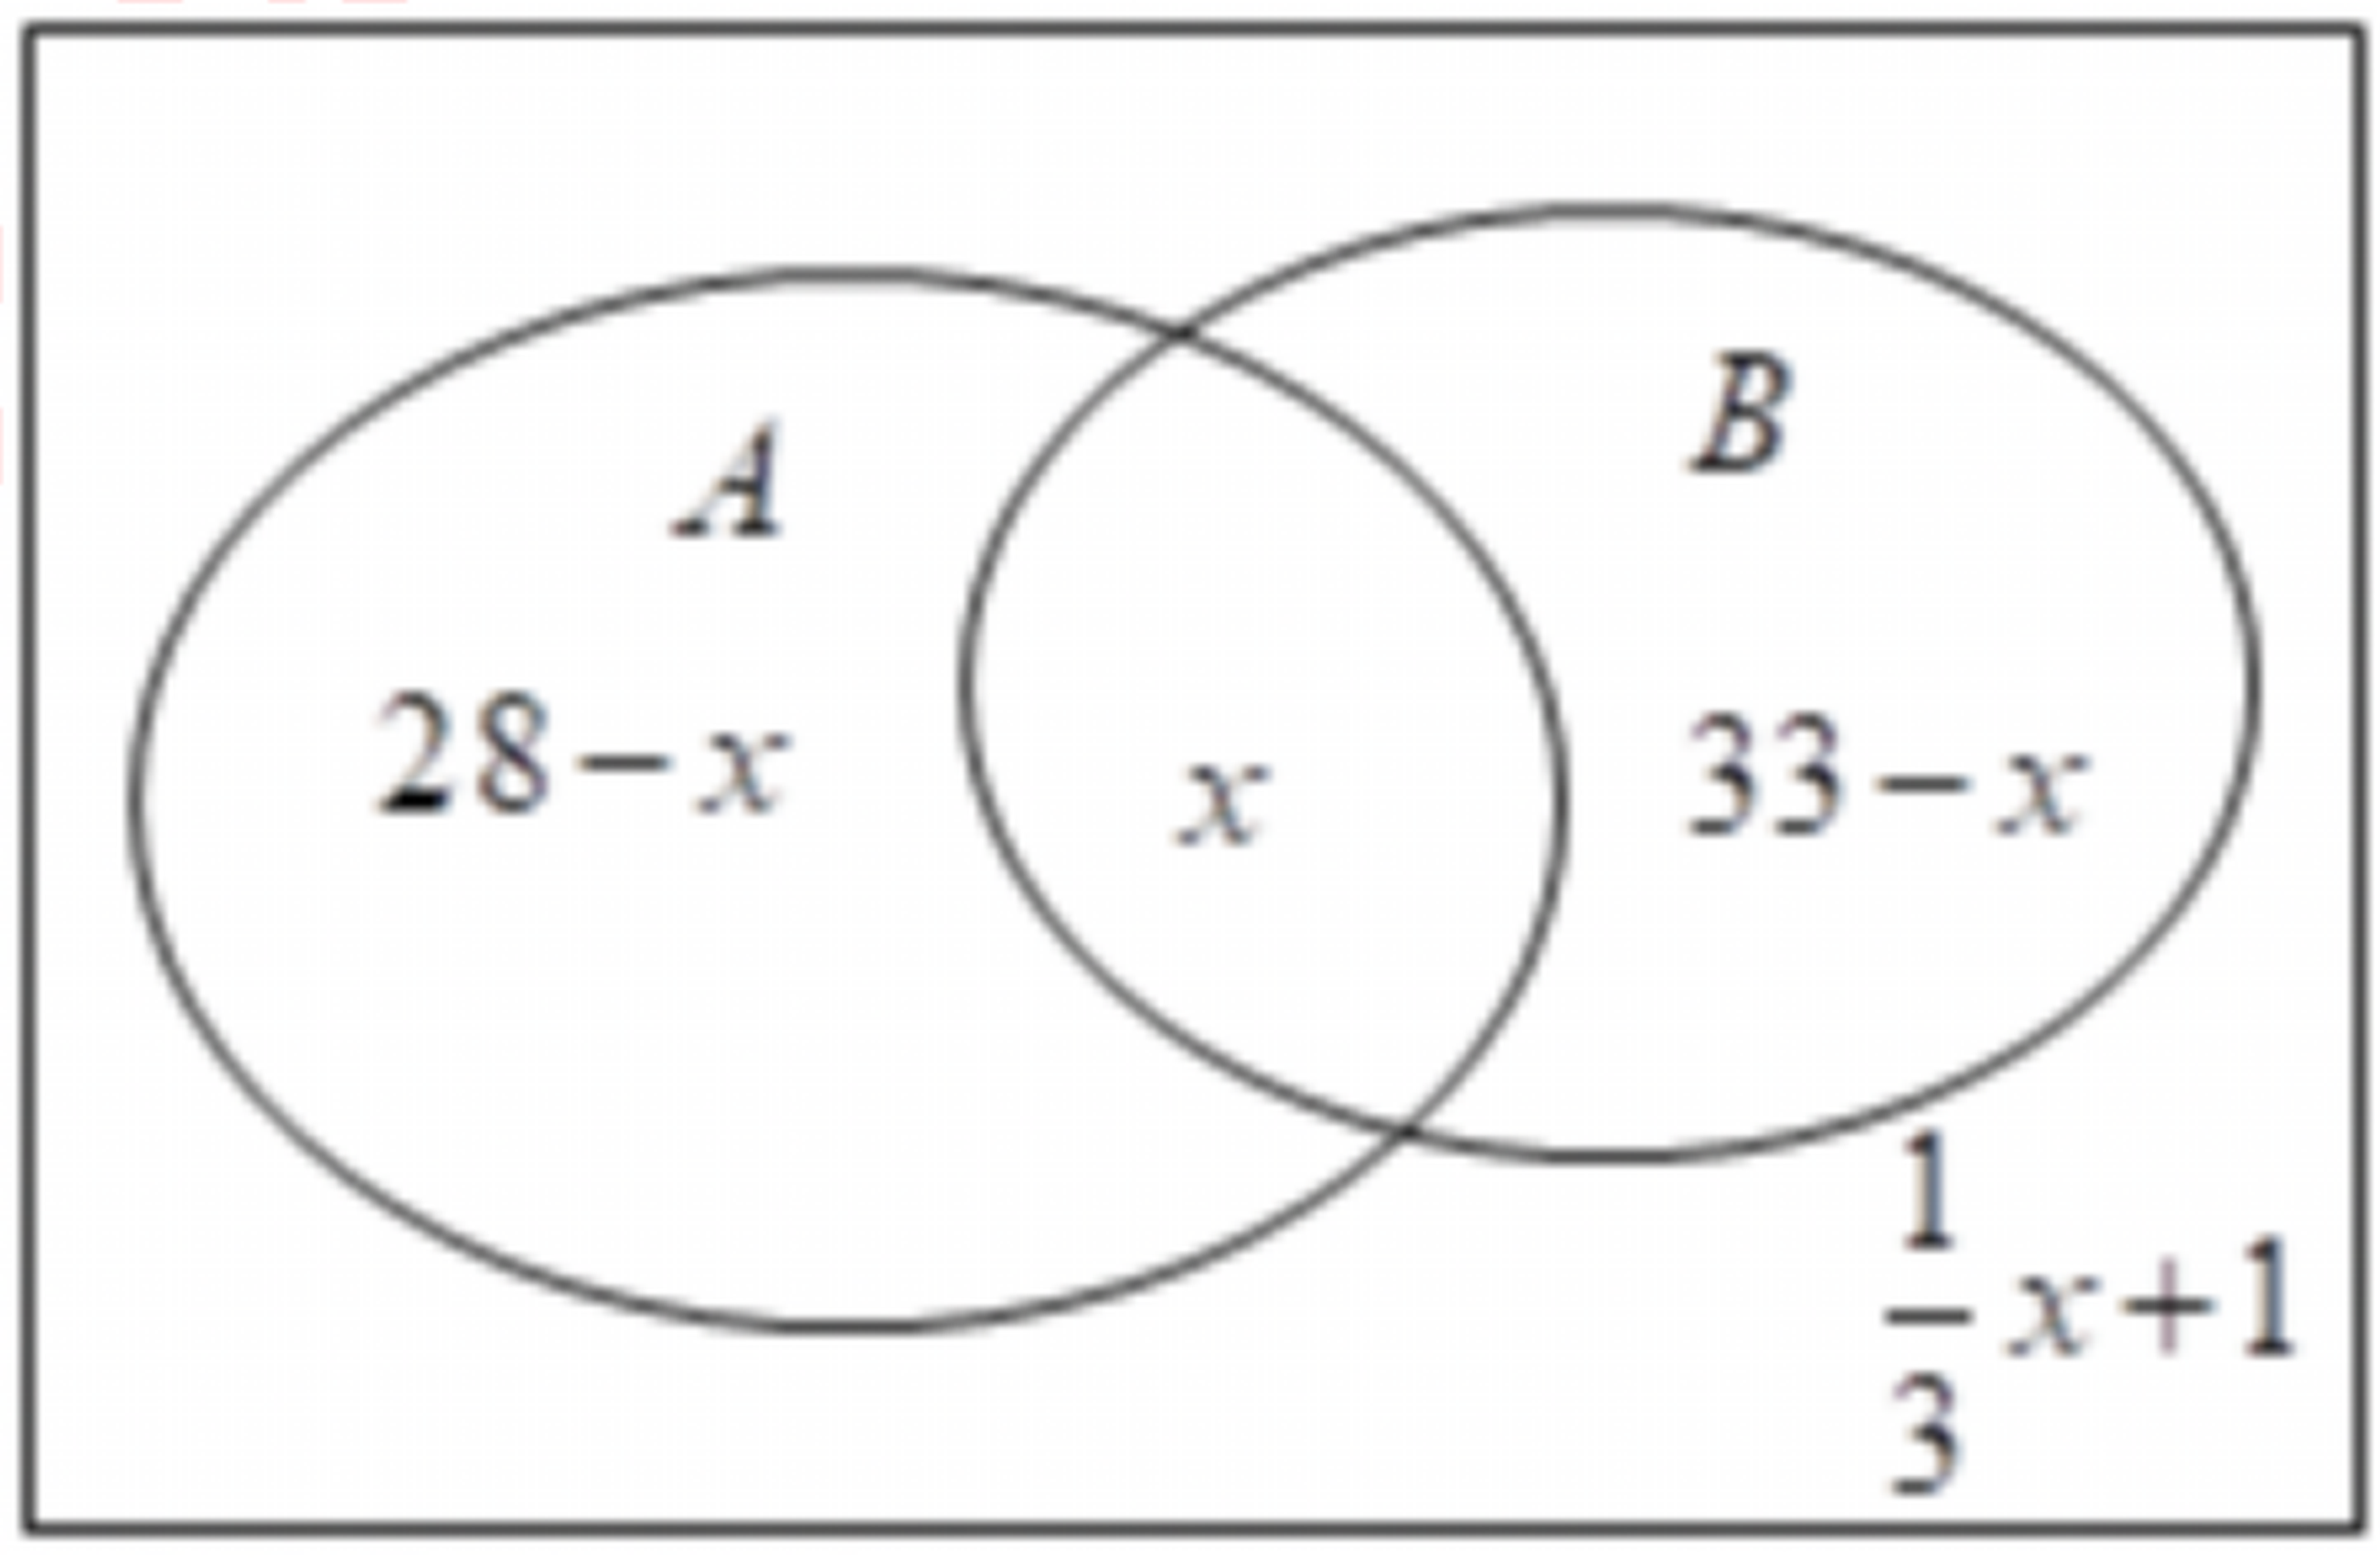
\includegraphics[width=0.42\textwidth]{figures/venn_AB_survey_50_x.png}
\end{center}
\step{则仅参加 $A$ 项的有 $(28-x)$ 人，仅参加 $B$ 项的有 $(33-x)$ 人，}
\step{$A$、$B$ 两项公益活动都不参加的有 $\left(\dfrac13x+1\right)$ 人，}
\step{由题意得 $x+(28-x)+(33-x)+\left(\dfrac13x+1\right)=50$，解得 $x=18$，}
\step{所以只参加 $A$ 项不参加 $B$ 项的有 $28-18=10$ 人.}
\solend
\fi

\item 设集合 $A=\{x\mid x^2-3x+2=0\}$，则满足 $A\cup B=\{0,1,2\}$ 的集合 $B$ 的个数是 \blankline[4.4em].

\ans{$4$}

\ifanswer
\solbegin
\step{$A=\{x\mid x^2-3x+2=0\}=\{x\mid x=1\text{ 或 }x=2\}=\{1,2\}$，}
\step{若 $A\cup B=\{0,1,2\}$，则 $0\in B$，}
\step{则 $B=\{0\},\{0,2\},\{1,0\},\{0,1,2\}$，共 $4$ 个.}
\solend
\fi

\item 已知全集 $U=\R$，集合 $A=\{x\mid x^2<4\}$，$B=\{y\mid y=x^2\}$，则图中阴影部分所表示的集合为 \blankline[4.4em].

\begin{center}
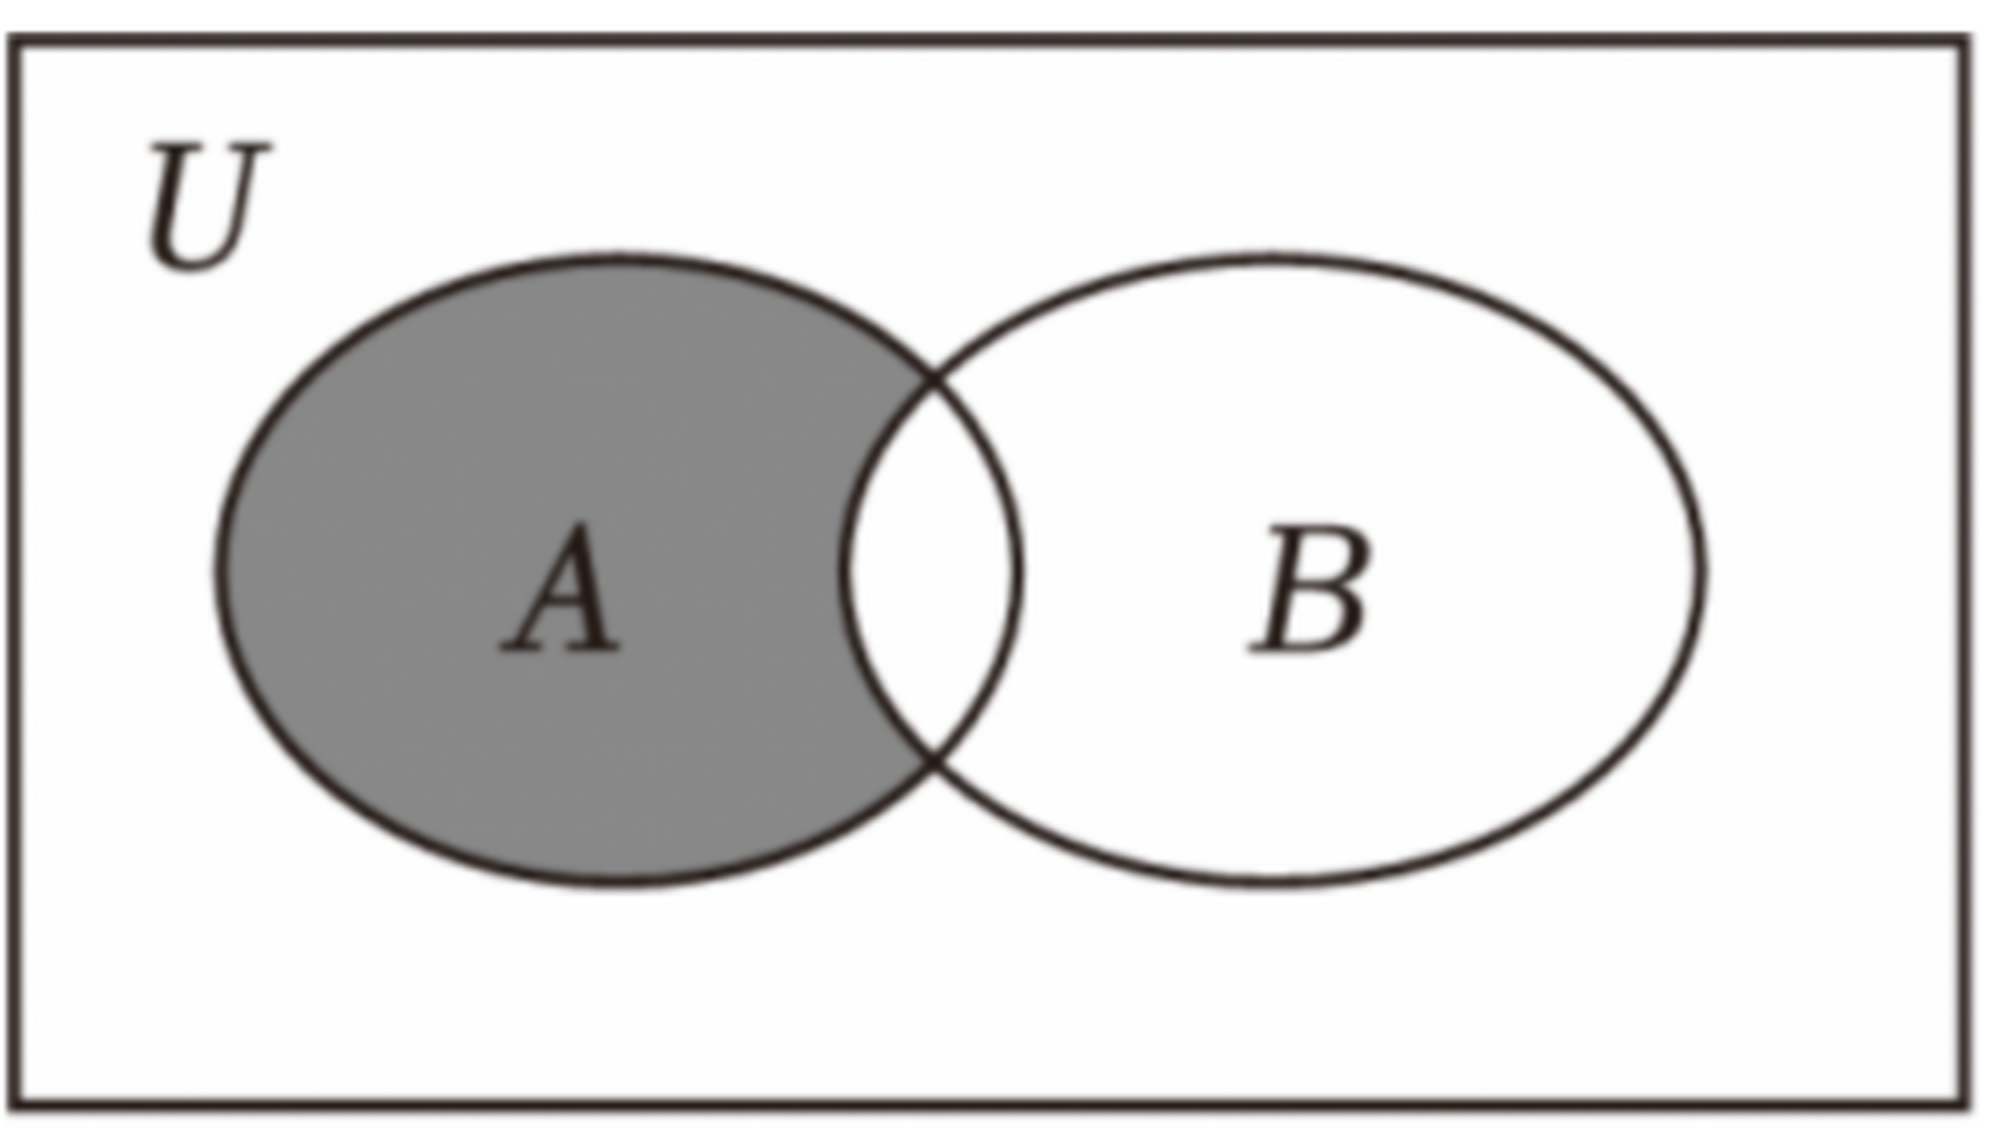
\includegraphics[width=0.34\textwidth]{figures/venn_A_shaded_U.png}
\end{center}

\ans{$A\cap\overline B=(-2,0)$}

\ifanswer
\solbegin
\step{集合 $A=\{x\mid x^2<4\}=(-2,2)$，$B=\{y\mid y=x^2\}=[0,+\infty)$，}
\step{图中阴影部分所表示的集合是 $A\cap\overline B=(-2,0)$.}
\solend
\fi

\item 如图所示，$M$、$P$、$S$ 是 $V$ 的三个子集，则阴影部分所表示的集合是 \blankline[5.4em].

\begin{center}
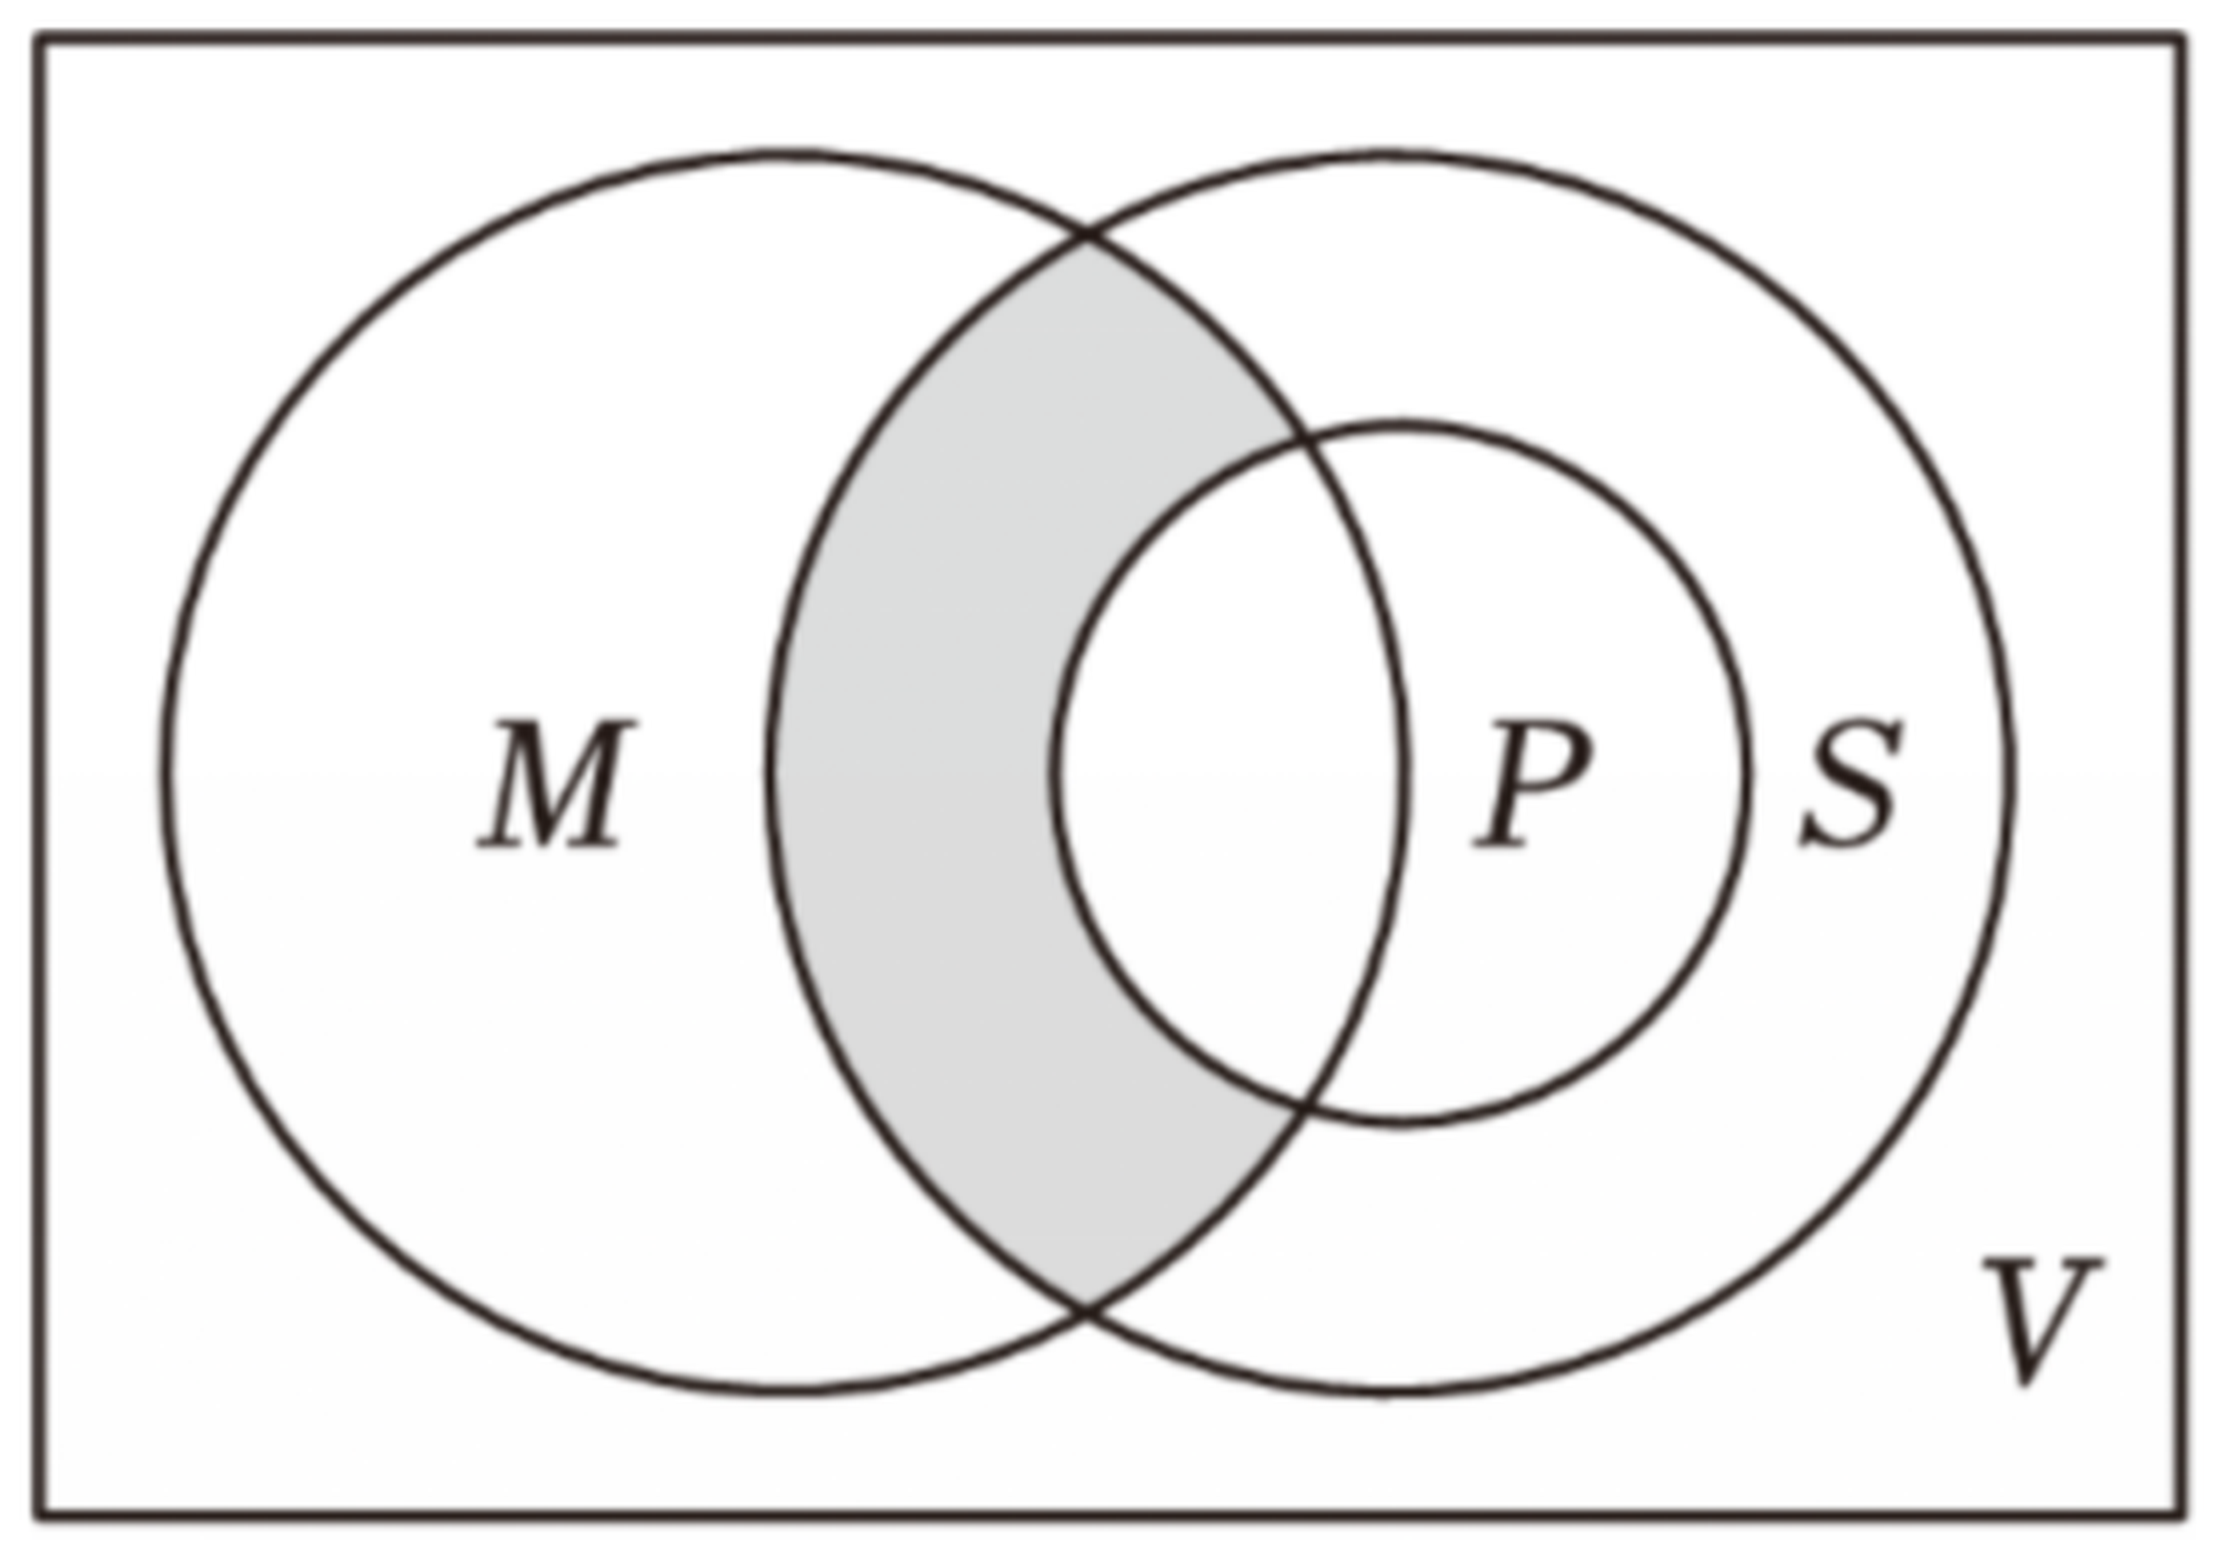
\includegraphics[width=0.38\textwidth]{figures/venn_MPS_V.png}
\end{center}

\ans{$(M\cap S)\cap(\complement_V P)$}

\item 下面六个关系式：① $\varnothing\subseteq\{a\}$；② $a\subseteq\{a\}$；③ $\{a\}\subseteq\{a\}$；④ $\{a\}\in\{a,b\}$；⑤ $a\in\{a,b,c\}$；⑥ $\varnothing\in\{a,b\}$；其中正确的是 \blankline[3.4em].

\ans{①③⑤}

\item 已知集合 $A=\{x\mid -1\le x\le a\}\ne\varnothing$，若 $\{y\mid y=x+1,x\in A\}=\{y\mid y=x^2,x\in A\}$，则实数 $a$ 值为 \blankline[4.4em].

\ans{$0$ 或 $\dfrac{1+\sqrt5}{2}$}

\ifanswer
\solbegin
\step{因为 $A=\{x\mid -1\le x\le a\}\ne\varnothing$，}
\step{所以 $\{y\mid y=x+1,x\in A\}=\{y\mid 0\le y\le a+1\}$，}
\step{$-1\le a\le1$ 时，$\{y\mid y=x^2,x\in A\}=\{y\mid 0\le y\le1\}$，}
\step{$a>1$ 时，$\{y\mid y=x^2,x\in A\}=\{y\mid 0\le y\le a^2\}$，}
\step{① $-1\le a\le1$ 时，$\{y\mid 0\le y\le a+1\}=\{y\mid 0\le y\le1\}$，则 $a+1=1$，解得 $a=0$；}
\step{② $a>1$ 时，$\{y\mid 0\le y\le a+1\}=\{y\mid 0\le y\le a^2\}$，则 $a^2=a+1$，解得 $a=\dfrac{1+\sqrt5}{2}$；}
\step{所以 $a=0$ 或 $\dfrac{1+\sqrt5}{2}$.}
\solend
\fi

\item 设集合 $A=\{(x,y)\mid x+y=22,x>0,y>0,x,y\text{ 均为质数}\}$ 的子集的个数为 \blankline[4.4em].

\ans{$32$}

\ifanswer
\solbegin
\step{集合 $A=\{(x,y)\mid x+y=22,x>0,y>0,x,y\text{ 均为质数}\}$}
\step{$=\{(3,19),(19,3),(5,17),(17,5),(11,11)\}$，则 $A$ 的子集的个数为 $2^5=32$.}
\solend
\fi

% 注：原卷本题题干印作「已知一个有四个数字元素的集合 $S$」；「数字元素」疑为「元素」之衍，
%     但原卷字形确为「数字」二字（已 3× 放大核对过），本稿照录，不代为改写。
\item 已知一个有四个数字元素的集合 $S$，$S$ 的所有子集的元素和（空集的元素和认为是 $0$）的总和为 $16192$，则 $S$ 的元素之和等于 \blankline[4.4em].

\ans{$2024$}

\ifanswer
\solbegin
\step{设 $S=\{a_1,a_2,a_3,a_4\}$，$S$ 的每个元素在所有子集中均出现 $2^3$ 次，}
\step{故 $(a_1+a_2+a_3+a_4)\cdot 2^3=16192$，所以 $a_1+a_2+a_3+a_4=2024$，}
\step{故 $S$ 的元素之和等于 $2024$.}
\solend
\fi

\item 设 $A$ 是非空数集，若对任意 $x$、$y\in A$，都有 $x+y\in A$、$xy\in A$，则称 $A$ 具有性质 $P$，给出以下命题：

①若 $A$ 具有性质 $P$，则 $A$ 可以是有限集；

②若 $A$ 具有性质 $P$，且 $A\ne\R$，则 $\overline A$ 具有性质 $P$；

③若 $A_1$、$A_2$ 具有性质 $P$，且 $A_1\cap A_2\ne\varnothing$，则 $A_1\cap A_2$ 具有性质 $P$；

④若 $A_1$、$A_2$ 具有性质 $P$，则 $A_1\cap A_2$ 具有性质 $P$.

其中所有真命题的序号是 \blankline[4.4em].

\ans{①③}

\ifanswer
\solbegin
\step{对于①，取集合 $A=\{0,1\}$ 具有性质 $P$，故 $A$ 可以是有限集，故①正确；}
\step{对于③，取 $x$、$y\in A_1\cap A_2$，则 $x\in A_1$，$x\in A_2$，$y\in A_1$，$y\in A_2$，}
\step{又 $A_1$、$A_2$ 具有性质 $P$，所以 $x+y\in A_1$，$xy\in A_1$，$x+y\in A_2$，$xy\in A_2$，}
\step{所以 $x+y\in A_1\cap A_2$，$xy\in A_1\cap A_2$，所以 $A_1\cap A_2$ 具有性质 $P$，故③正确；}
\step{对于④，取 $A_1=\{x\mid x=2k,k\in\Z\}$，$A_2=\{x\mid x=3k,k\in\Z\}$，$2\in A_1$，$3\in A_2$，}
\step{但 $2+3\notin A_1\cup A_2$，故④错误；}
\step{对于②，若 $A$ 具有性质 $P$，且 $A\ne\R$，假设 $\overline A$ 也具有性质 $P$，}
\step{设 $0\in A$，在 $\overline A$ 中任取一个 $x$，$x\ne0$，此时可证得 $-x\in A$，}
\step{否则若 $-x\in\overline A$，由于 $\overline A$ 也具有性质 $P$，则 $x+(-x)=0\in\overline A$，}
\step{与 $0\in A$ 矛盾，故 $-x\in A$，}
\step{由于 $A$ 具有性质 $P$，$\overline A$ 也具有性质 $P$，所以 $(-x)^2\in A$，$x^2\in\overline A$，}
\step{而 $(-x)^2=x^2$，这与 $A\cap\overline A=\varnothing$ 矛盾，}
\step{故当 $0\in A$ 且 $A$ 具有性质 $P$ 时，则 $\overline A$ 不具有性质 $P$，}
\step{同理当 $0\in\overline A$ 时，也可以类似推出矛盾，故②错误.}
\step{故正确的是①③.}
\solend
\fi

\item 已知 $S=\{1,2,3,4,5\}$，$A=\{1,2,5\}$，$T=\{t_1,t_2\}\subseteq S$，记 $A_1=\{x\mid x=a+t_1,a\in A,t_1\in T\}$，$A_2=\{x\mid x=b+t_2,b\in A,t_2\in T\}$，若 $A_1\cap A_2=\varnothing$，则集合 $T$ 为 \blankline[5.4em].

\ans{$T=\{1,3\}$ 或 $T=\{2,4\}$ 或 $T=\{3,5\}$}

\ifanswer
\solbegin
\step{若 $A_1\cap A_2=\varnothing$，即 $a+t_1\ne b+t_2$，则 $t_1-t_2\ne a-b$，其中 $a$、$b\in A$，}
\step{否则 $t_1+a=t_2+b$，$A_1\cap A_2\ne\varnothing$，}
\step{又 $S=\{1,2,3,4,5\}$，$A=\{1,2,5\}$，$T=\{t_1,t_2\}\subseteq S$，}
\step{$2-1=1$，$5-2=3$，$5-1=4$，则 $t_1$、$t_2$ 相差 $2$，}
\step{所以 $T=\{1,3\}$ 或 $T=\{2,4\}$ 或 $T=\{3,5\}$.}
\solend
\fi

\end{enumerate}

\bigsec{二、解答题}

\begin{enumerate}
\setcounter{enumi}{13}

\item 设集合 $P=\{1,2,3,m\}$，$Q=\{3,m^2\}$，且 $\overline P\cap Q=\varnothing$，求实数 $m$ 的值组成的集合.

\ans{$\{-1,0,\pm\sqrt2\}$}

\ansspace[5]

\ifanswer
\solbegin
\step{因为 $\overline P\cap Q=\varnothing$，所以 $Q\subseteq P$，所以 $m^2=1$ 或 $m^2=2$ 或 $m^2=m$，}
\step{考虑互异性，得 $m=-1$ 或 $m=\pm\sqrt2$ 或 $m=0$，}
\step{所以实数 $m$ 的值组成的集合为 $\{-1,0,\pm\sqrt2\}$.}
\solend
\fi

\item 若集合 $A=(-\infty,2]$，$B=\{x\mid kx+1<0,k\in\R\}$，$A\cap B=\varnothing$，求实数 $k$ 的取值范围.

\ans{$\left[-\dfrac12,0\right]$}

\ansspace[5]

\ifanswer
\solbegin
\step{若 $B=\varnothing$，则 $k=0$，符合题意，}
\step{若 $B\ne\varnothing$，当 $k>0$ 时，$B=\left(-\infty,-\dfrac1k\right)$，$A\cap B\ne\varnothing$，不合题意；}
\step{当 $k<0$ 时，$B=\left(-\dfrac1k,+\infty\right)$，由 $A\cap B=\varnothing$ 得 $-\dfrac1k\ge2$，即 $-\dfrac12\le k<0$，}
\step{故 $k$ 的取值范围是 $\left[-\dfrac12,0\right]$.}
\solend
\fi

\item 已知集合 $A=\{-4,2a-1,a^2\}$，$B=\{a-5,1-a,9\}$，分别求适合下列条件的 $a$ 的值.

% 两个小问不许与题干分家：试卷版第 2 页页末原本正好把 (1) 留在页底、(2) 翻到次页，
% 与 2026-09-15 修的三类难看切页同源，故在这里也加 \keepwithprev 守卫（三版都生效）。
\keepwithprev
（1）$9\in(A\cap B)$；

\keepwithprev
（2）$\{9\}=A\cap B$.

\ans{（1）$a=5$ 或 $a=-3$；（2）$a=-3$}

\ansspace[5]

\ifanswer
\solbegin
\stepm{（1）}{$9\in(A\cap B)$，所以 $9\in A$，}
\step{当 $2a-1=9$ 时，$a=5$，当 $a^2=9$ 时，即 $a=\pm3$，}
% 注：原卷此句结论印作「所以 $a$ 的值为 $5\backslash-3$」——「\」应是顿号之误，
%     本稿照录原卷字形（见文件头「原卷存疑」②）；按文意即 $a=5$ 或 $a=-3$。
\step{当 $a=3$ 时，$a-5=1-a$ 舍去，所以 $a$ 的值为 $5\backslash-3$.}
\stepm{（2）}{结合（1）的结论：}
\step{当 $2a-1=9$ 即 $a=5$ 时，$1-a=-4$，$\{9\}\ne(A\cap B)$，}
\step{当 $a^2=9$ 时，即 $a=\pm3$，当 $a=3$ 时，$a-5=1-a$ 舍去，}
\step{所以 $a$ 的值为 $-3$.}
\solend
\fi

\item 已知集合 $M=\{a,ab,a-b\}$，$N=\{0,|a|,b\}$，且 $M=N$，求实数 $a$、$b$ 的值.

\ans{$a=b=-1$}

\ansspace[5]

\ifanswer
\solbegin
\step{由集合元素的互异性，得 $a\ne0$，且 $b\ne0$，所以 $a-b=0$，即 $a=b$，}
\step{所以 $ab=|a|$，又由 $|a|\ne b=a$，得 $a<0$，故 $a=b=-1$.}
\solend
\fi

\item 已知集合 $A=\{x\mid -2<x<7\}$，$B=\{x\mid m+1\le x\le 2m-1\}$.

\keepwithprev
（1）当 $m=4$ 时，求 $A\cap B$、$A\cup B$；

\keepwithprev
（2）若 $A\cap B=B$，求实数 $m$ 的取值范围.

\ans{（1）$A\cap B=[5,7)$，$A\cup B=(-2,7]$；（2）$(-\infty,4)$}

\ansspace[5]

\ifanswer
\solbegin
\stepm{（1）}{当 $m=4$ 时，得集合 $A=\{x\mid -2<x<7\}$，$B=\{x\mid 5\le x\le7\}$，}
\step{得 $A\cap B=[5,7)$，$A\cup B=(-2,7]$.}
\stepm{（2）}{由 $A\cap B=B$ 得 $B\subseteq A$，}
\step{①当 $B=\varnothing$ 时，得 $m+1>2m-1$，解得 $m<2$；}
\step{②当 $B\ne\varnothing$ 时，得 $\begin{cases}m+1>-2\\ 2m-1<7\\ m+1\le2m-1\end{cases}$，解得 $2\le m<4$；}
\step{综上，实数 $m$ 的取值范围是 $(-\infty,4)$.}
\solend
\fi

\item 若集合 $A=\{x\mid x^2+5x-6=0\}$，$B=\{x\mid x^2+2(m+1)x+m^2-3=0\}$.

\keepwithprev
（1）当 $m=0$ 时，求集合 $A\cup B$；

\keepwithprev
（2）若 $A\cap B=B$，求实数 $m$ 的取值范围.

\ans{（1）$A\cup B=\{1,-6,-3\}$；（2）$\{m\mid m\le-2\}$}

\ansspace[5]

\ifanswer
\solbegin
\stepm{（1）}{由题意得，集合 $A=\{x\mid x^2+5x-6=0\}=\{1,-6\}$，}
\step{当 $m=0$ 时，$B=\{x\mid x^2+2x-3=0\}=\{1,-3\}$，}
\step{所以 $A\cup B=\{1,-6,-3\}$；}
\stepm{（2）}{由（1）得集合 $A=\{1,-6\}$，$B=\{x\mid x^2+2(m+1)x+m^2-3=0\}$，}
\step{若 $A\cap B=B$ 得 $B\subseteq A$，所以 $B=\varnothing$ 或 $\{-6\}$ 或 $\{1\}$ 或 $\{1,-6\}$，}
\step{当 $B=\varnothing$ 时，$\Delta=4(m+1)^2-4(m^2-3)<0$，解得 $m<-2$，}
\step{当 $B=\{-6\}$ 时，则 $\begin{cases}\Delta=4(m+1)^2-4(m^2-3)=0\\ 36-12(m+1)+m^2-3=0\end{cases}$，无解，}
\step{当 $B=\{1\}$ 时，则 $\begin{cases}\Delta=4(m+1)^2-4(m^2-3)=0\\ 1+2(m+1)+m^2-3=0\end{cases}$，解得 $m=-2$，}
\step{当 $B=\{1,-6\}$ 时，则 $\begin{cases}\Delta=4(m+1)^2-4(m^2-3)>0\\ 1+(-6)=-2(m+1)\\ 1\times(-6)=m^2-3\end{cases}$，无解，}
\step{综上所述，实数 $m$ 的取值范围为 $\{m\mid m\le-2\}$.}
\solend
\fi

% 压轴题：其后已无内容，故作答区全用可丢弃胶水（\ansspace*），并在题目前先量一下版面。
\ansneed{8cm}
\item 对于点集 $A=\{(x,y)\mid x=m,y=-3x+2,m\in\N,m\ge1\}$，$B=\{(x,y)\mid x=n,y=a(x^2-x+1),n\in\N,n\ge1\}$，是否存在非零整数 $a$，使得 $A\cap B\ne\varnothing$？

\ans{$a=-1$}

\ansspace*[10]

\ifanswer
\solbegin
\step{当 $A\cap B\ne\varnothing$ 时，$-3x+2=a(x^2-x+1)$，}
\step{$ax^2+(3-a)x+a-2=0$ ①有正整数解，}
\step{所以 $\Delta=(3-a)^2-4a(a-2)=-3a^2+2a+9$ 是平方数，}
\step{所以 $3a^2-2a-9\le0$，$\dfrac{1-2\sqrt7}{3}\le a\le\dfrac{1+2\sqrt7}{3}$，$a\ne0$，$a\in\Z$，}
\step{所以 $a=\pm1$ 或 $a=2$，}
\step{$a=-1$ 时 $\Delta=4$，这时①变为 $-x^2+4x-3=0$，解得 $x_1=1$，$x_2=3$，}
\step{$A\cap B=\{(1,-1),(3,-7)\}$.}
\step{$a=1$ 时 $\Delta=8$，不是平方数.}
\step{$a=2$ 时 $\Delta=1$，这时①变为 $2x^2+x=0$，没有正整数解.}
\step{所以 $a=-1$.}
\solend
\fi

\end{enumerate}

\end{document}
"
% 紧凑版：xelatex "\def\iscompact{1}% 高一19_延安中学_周末作业2.tex —— 高一上数学「2026-2027 年延安中学高一上周末作业 2」（试卷版/答案版）
% 试卷版：xelatex 高一19_延安中学_周末作业2.tex
% 答案版：xelatex "\def\isanswer{1}\input{高一19_延安中学_周末作业2.tex}"
% 紧凑版：xelatex "\def\iscompact{1}\input{高一19_延安中学_周末作业2.tex}"
%
% 原始材料是微信公众号图文（公众号「魔都数学加油站」，作者署名「破晓」，
% 原文链接 https://mp.weixin.qq.com/s/tHqWSV1StO5SHSXXQ4jeUA），正文为 6 张 PNG 页；
% 原文本身就是一份**讲评版**——题目下方直接印出【答案】或【解析】。本稿把答案与解析
% 移到答案版，试卷版即一张干净的空卷；试题文字、答案与解析均照原卷录入。
%
% 与原卷的排版差异（均已在 README「说明」中交代）：
%   ① 原文自**第 3 题**起（第 1、2 题未在该文发布），源码里以 \setcounter{enumi}{2} 起编；
%      全卷只有「一、填空题」「二、解答题」两节，无选择题；
%   ② 原卷本就印有两个分节标题（已在原图上逐页放大核对过），本稿照原卷分节，只把标题改排
%      成全稿统一的「大节标题」样式；
%   ③ 原卷的实数集、整数集、自然数集符号作正体 $R$、$Z$、$N$（第 15 题作粗体 $\mathbf{R}$，
%      第 20 题有 $N$ 与斜体 $Z$），本稿按全稿惯例统一写作 $\R$、$\Z$、$\N$；
%   ④ 第 4 题的韦恩图在原卷里印在【解析】右侧（题干并无「如图」二字），故本稿把该图放进
%      答案版的解析块内（`figures/venn_AB_survey_50_x.png`）；第 6、7 题的韦恩图是**题干图**
%      （题干作「图中阴影部分所表示的集合」），两版都排（`figures/venn_A_shaded_U.png`、
%      `figures/venn_MPS_V.png`）。三张图都取自原卷截图、4× LANCZOS 放大，不用 TikZ 手绘；
%   ⑤ 本卷也是「讲评版」，解析按全稿统一的 \solbegin/\step 分步重排（原卷为连续段落），
%      分步不改一字，只断句、断行；
%   ⑥ 标题前缀照**原卷**作「2026--2027 年…」（原卷标题即作「2026-2027年延安中学高一上周末
%      作业 2」）。同校的 高一06 作「学年度」——那是 高一02—高一09 那一批入库时统一改的；
%      后续入库的卷（高一10—高一17 与本卷）一律照原卷保留「年」，未强改，故同校两卷前缀不同。
%
% 原卷存疑两处（已逐处放大到能看清字形后核对，本稿照录并加注，见各题下的 `%` 注）：
%   （另有第三处「第 12 题【解析】末句」原先记作存疑，2026-09-26 第二轮核对放大后发现
%     原卷印的是「$0\in\overline A$」——A 上确有横杠，是本稿当初漏抄了 $\overline{}$；
%     已按原卷补回，故该条从存疑清单里删去，不计为原卷问题。）
%   ① 第 11 题题干印作「已知一个有四个数字元素的集合 $S$」，「数字元素」疑为「元素」之衍；
%   ② 第 16 题 (1) 结论印作「$a$ 的值为 $5\backslash-3$」，其中的「\」应是顿号之误
%      （由 (2) 的结论「$a$ 的值为 $-3$」可反推，(1) 的答案是 $5$ 或 $-3$）；

% 本篇在公众号「魔都数学加油站」连载里的编号是「27学年高一19」，本地编号与之对齐（高一19）；
% 对应关系见 README「与公众号连载号的对照表」。
\documentclass[a4paper,11pt]{article}
\usepackage{common}

\begin{document}

\examtitlest{2026--2027 年延安中学高一上周末作业 2}{集合与常用逻辑用语}

\bigsec{一、填空题}

\begin{enumerate}
% 原卷填空题从第 3 题起（1、2 未在该文中发布），须与解答题的 \setcounter{enumi}{13} 对齐
\setcounter{enumi}{2}
\item 已知全集 $U=\{1,2,3,4,5\}$，$M=\{1,2\}$，$P=\{1,3,5\}$，则 $M\cap\overline P=$ \blankline[4.4em].

\ans{$\{2\}$}

\item 某公司共有 $50$ 人，此次组织参加社会公益活动，其中参加 $A$ 项公益活动的有 $28$ 人，参加 $B$ 项公益活动的有 $33$ 人，且 $A$、$B$ 两项公益活动都不参加的人数比都参加的人数的三分之一多 $1$ 人，则只参加 $A$ 项不参加 $B$ 项的人数是 \blankline[4.4em].

\ans{$10$}

\ifanswer
\solbegin
\step{如图所示，设 $A$、$B$ 两项公益活动都参加的有 $x$ 人，}
\begin{center}
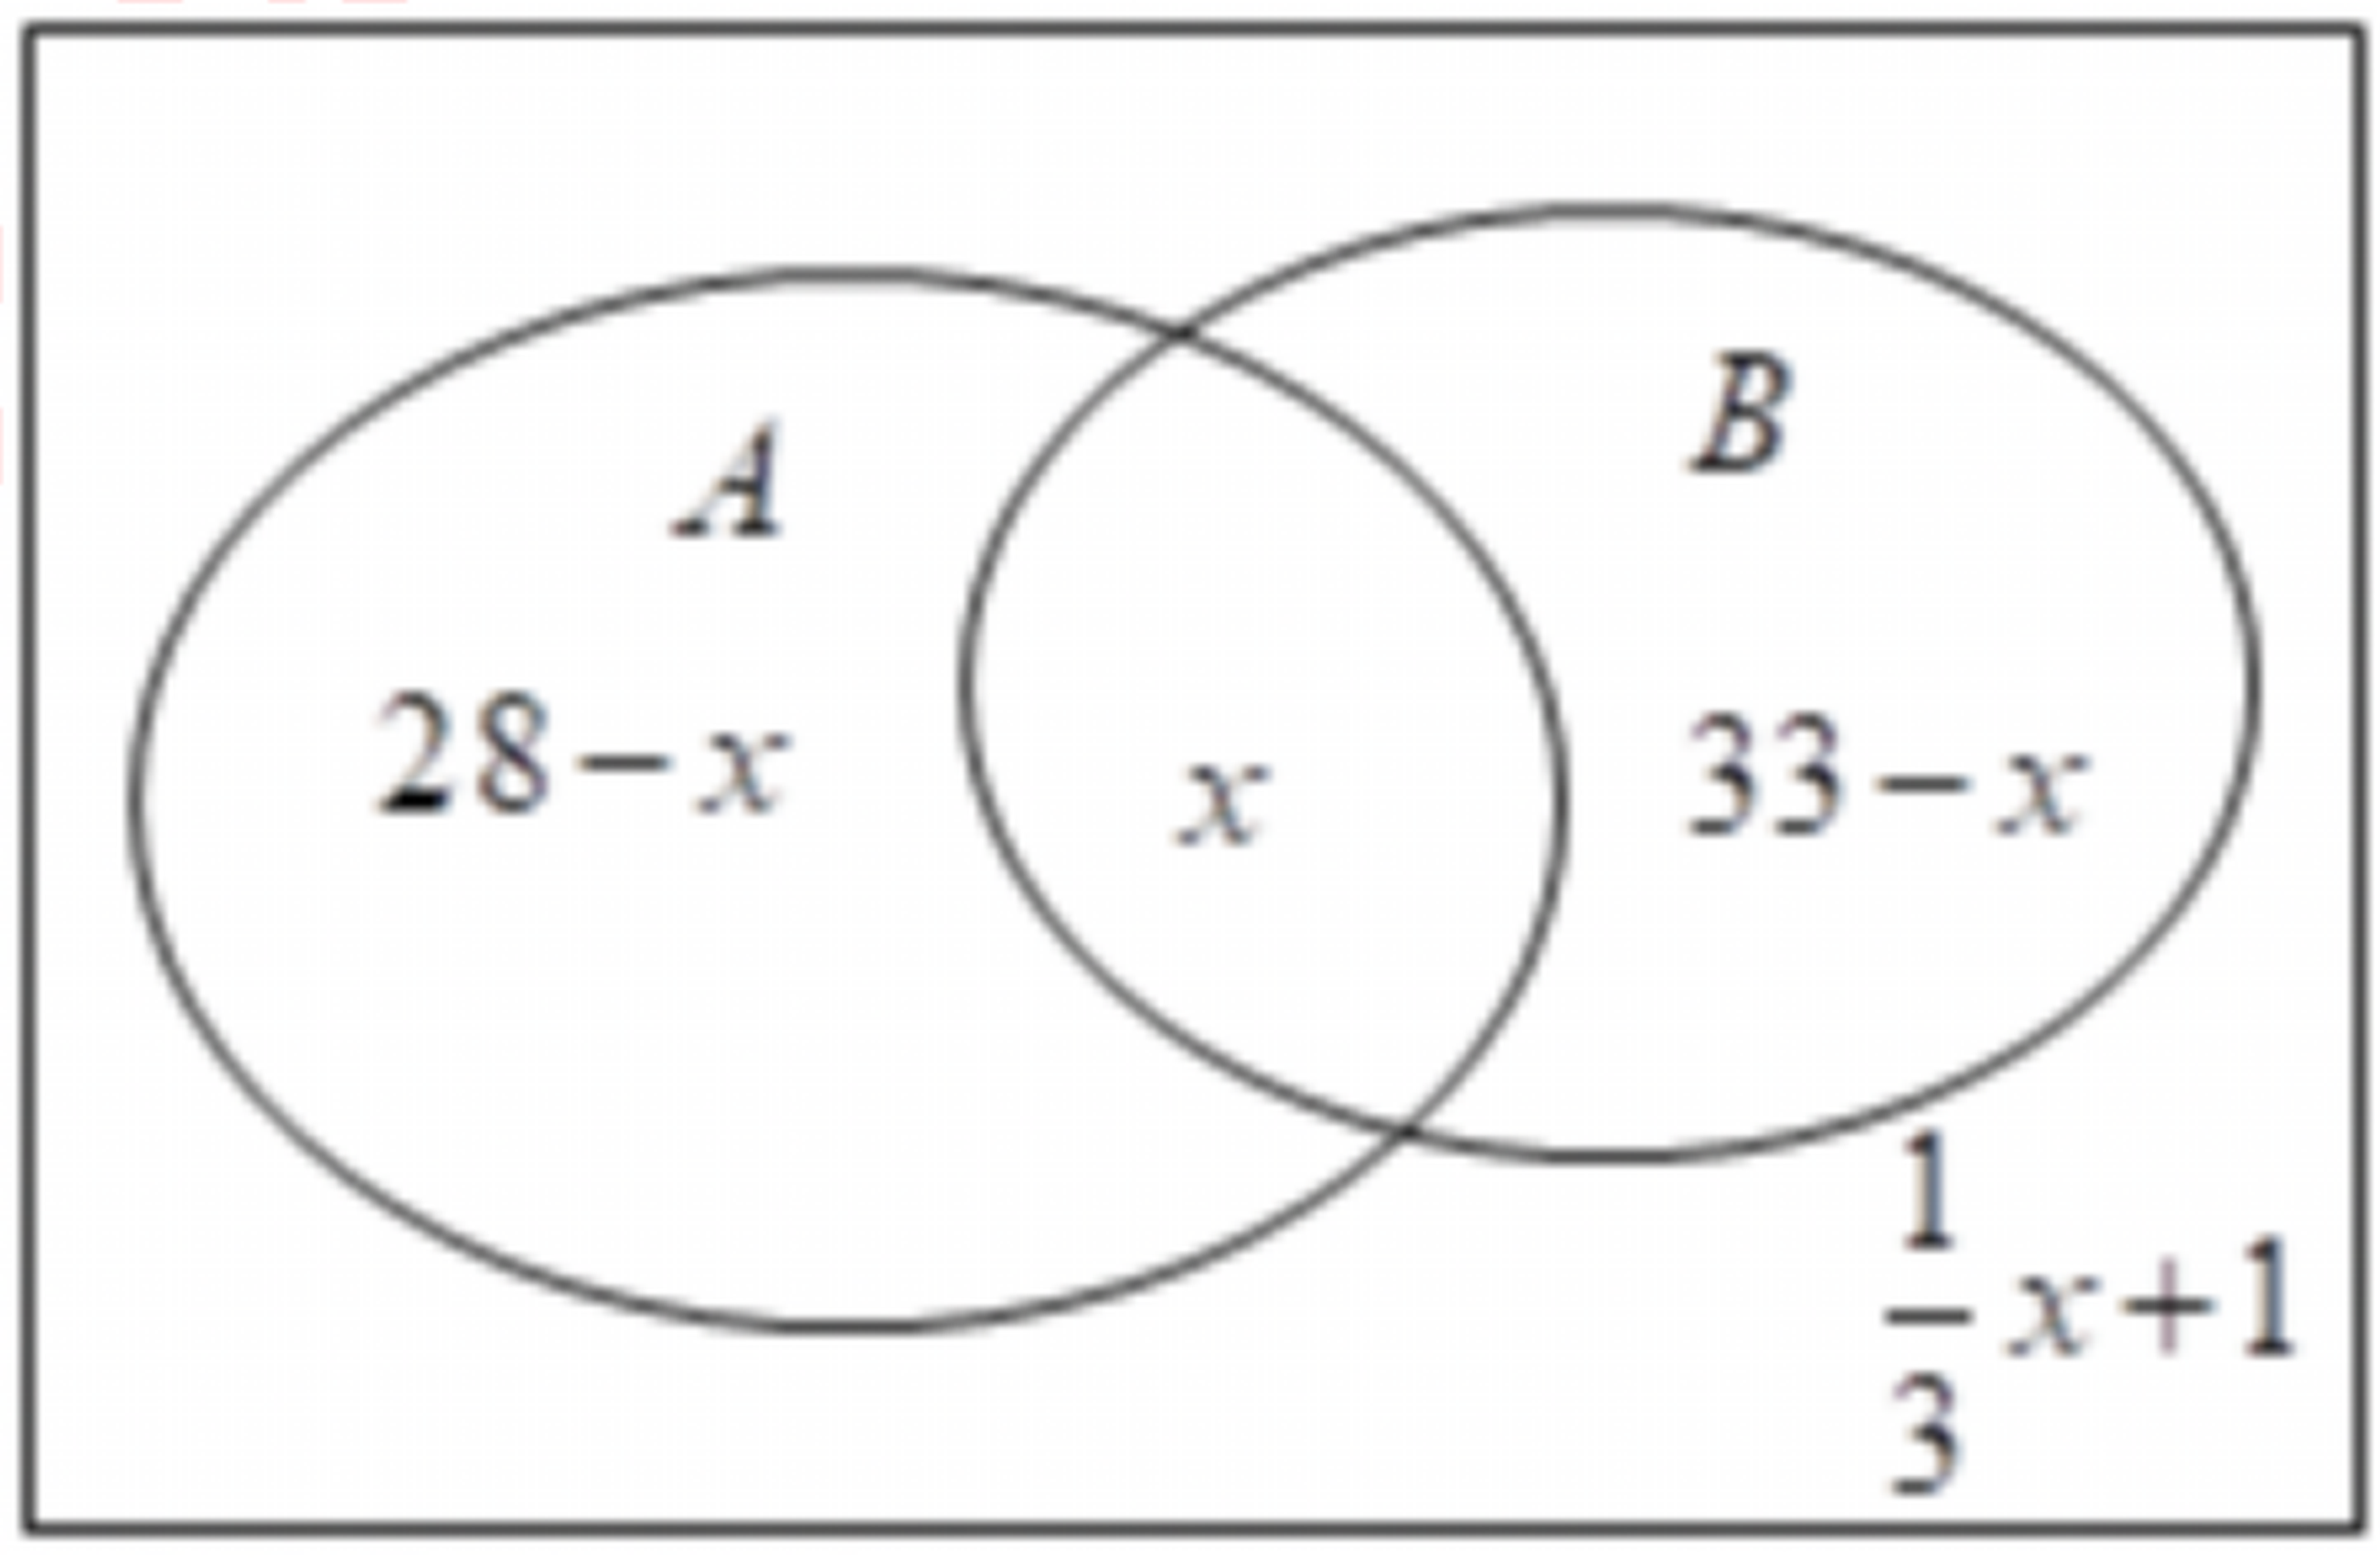
\includegraphics[width=0.42\textwidth]{figures/venn_AB_survey_50_x.png}
\end{center}
\step{则仅参加 $A$ 项的有 $(28-x)$ 人，仅参加 $B$ 项的有 $(33-x)$ 人，}
\step{$A$、$B$ 两项公益活动都不参加的有 $\left(\dfrac13x+1\right)$ 人，}
\step{由题意得 $x+(28-x)+(33-x)+\left(\dfrac13x+1\right)=50$，解得 $x=18$，}
\step{所以只参加 $A$ 项不参加 $B$ 项的有 $28-18=10$ 人.}
\solend
\fi

\item 设集合 $A=\{x\mid x^2-3x+2=0\}$，则满足 $A\cup B=\{0,1,2\}$ 的集合 $B$ 的个数是 \blankline[4.4em].

\ans{$4$}

\ifanswer
\solbegin
\step{$A=\{x\mid x^2-3x+2=0\}=\{x\mid x=1\text{ 或 }x=2\}=\{1,2\}$，}
\step{若 $A\cup B=\{0,1,2\}$，则 $0\in B$，}
\step{则 $B=\{0\},\{0,2\},\{1,0\},\{0,1,2\}$，共 $4$ 个.}
\solend
\fi

\item 已知全集 $U=\R$，集合 $A=\{x\mid x^2<4\}$，$B=\{y\mid y=x^2\}$，则图中阴影部分所表示的集合为 \blankline[4.4em].

\begin{center}
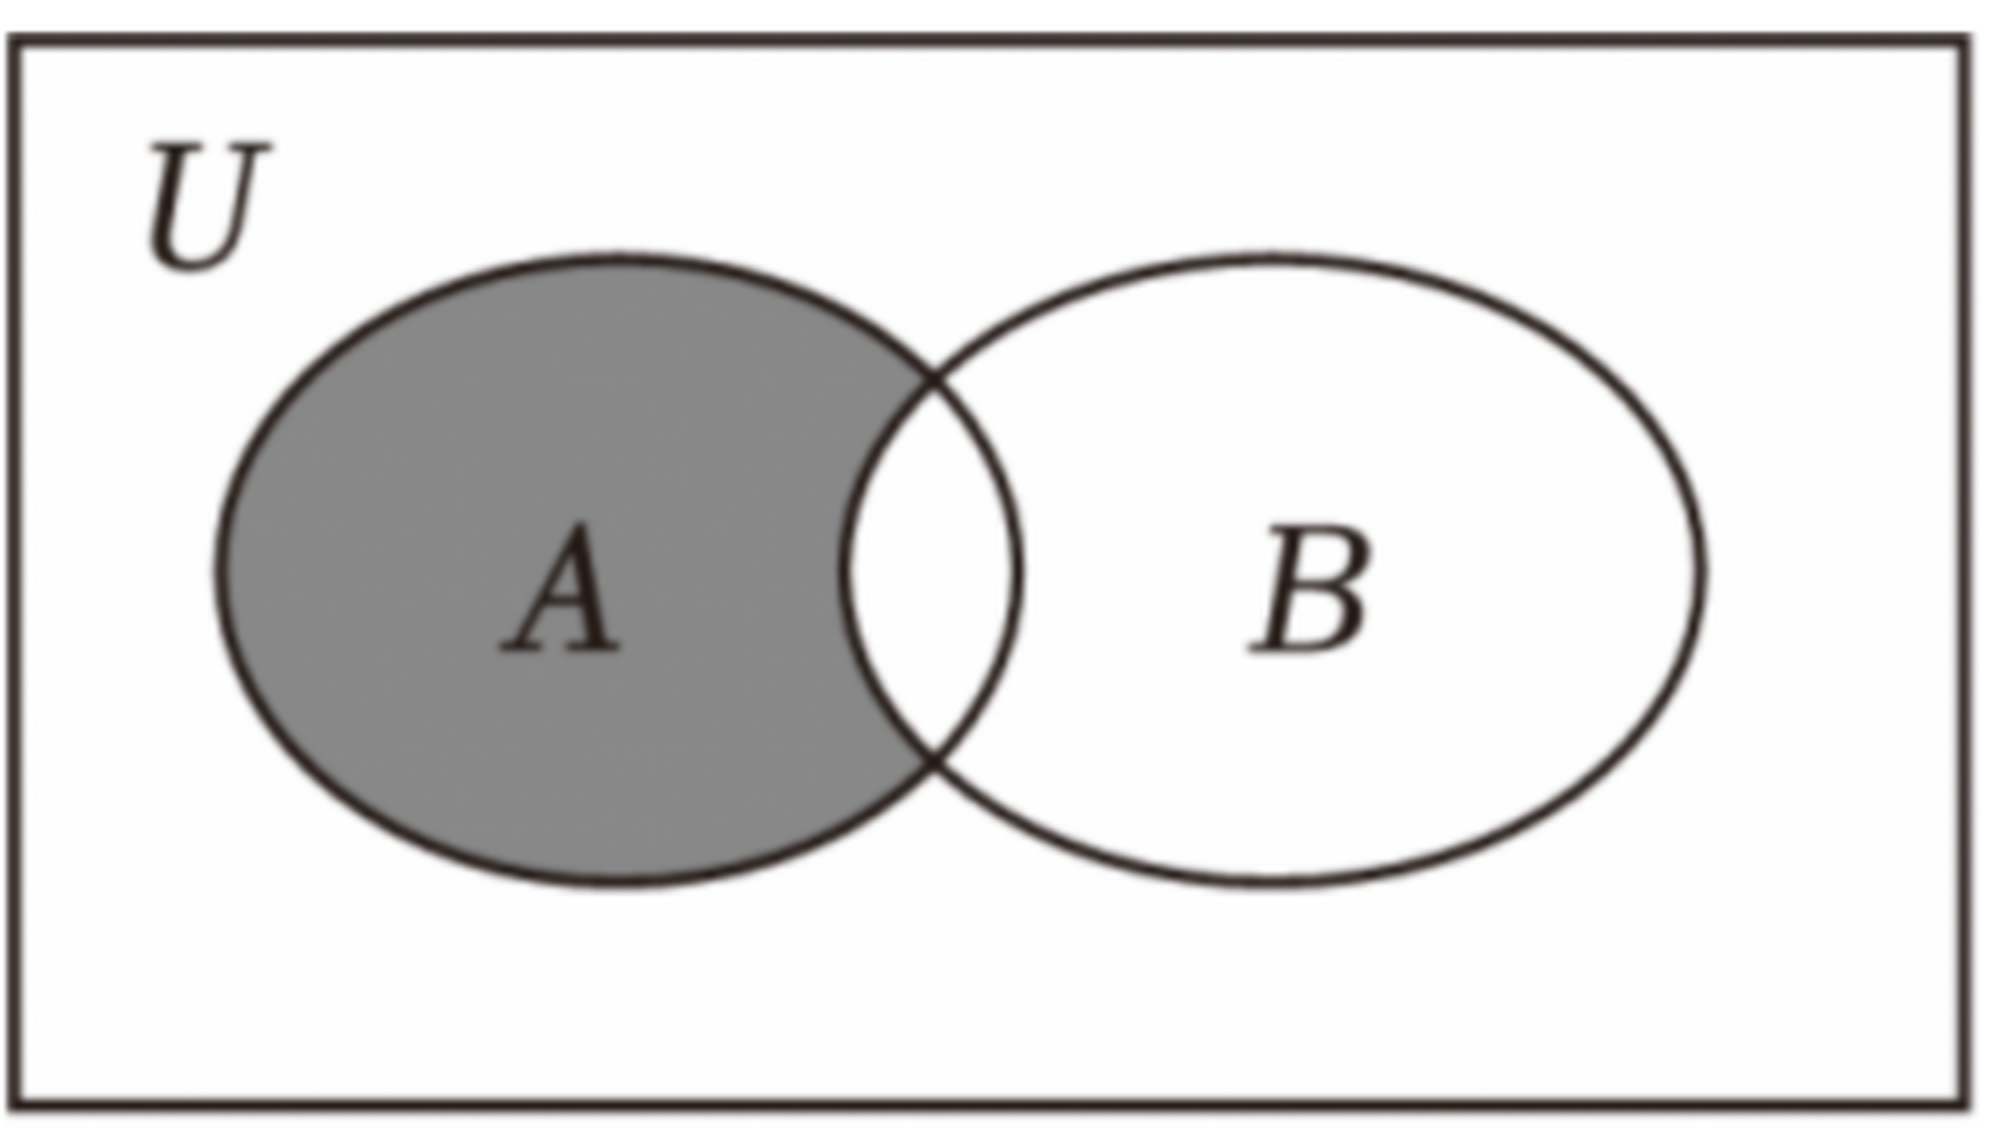
\includegraphics[width=0.34\textwidth]{figures/venn_A_shaded_U.png}
\end{center}

\ans{$A\cap\overline B=(-2,0)$}

\ifanswer
\solbegin
\step{集合 $A=\{x\mid x^2<4\}=(-2,2)$，$B=\{y\mid y=x^2\}=[0,+\infty)$，}
\step{图中阴影部分所表示的集合是 $A\cap\overline B=(-2,0)$.}
\solend
\fi

\item 如图所示，$M$、$P$、$S$ 是 $V$ 的三个子集，则阴影部分所表示的集合是 \blankline[5.4em].

\begin{center}
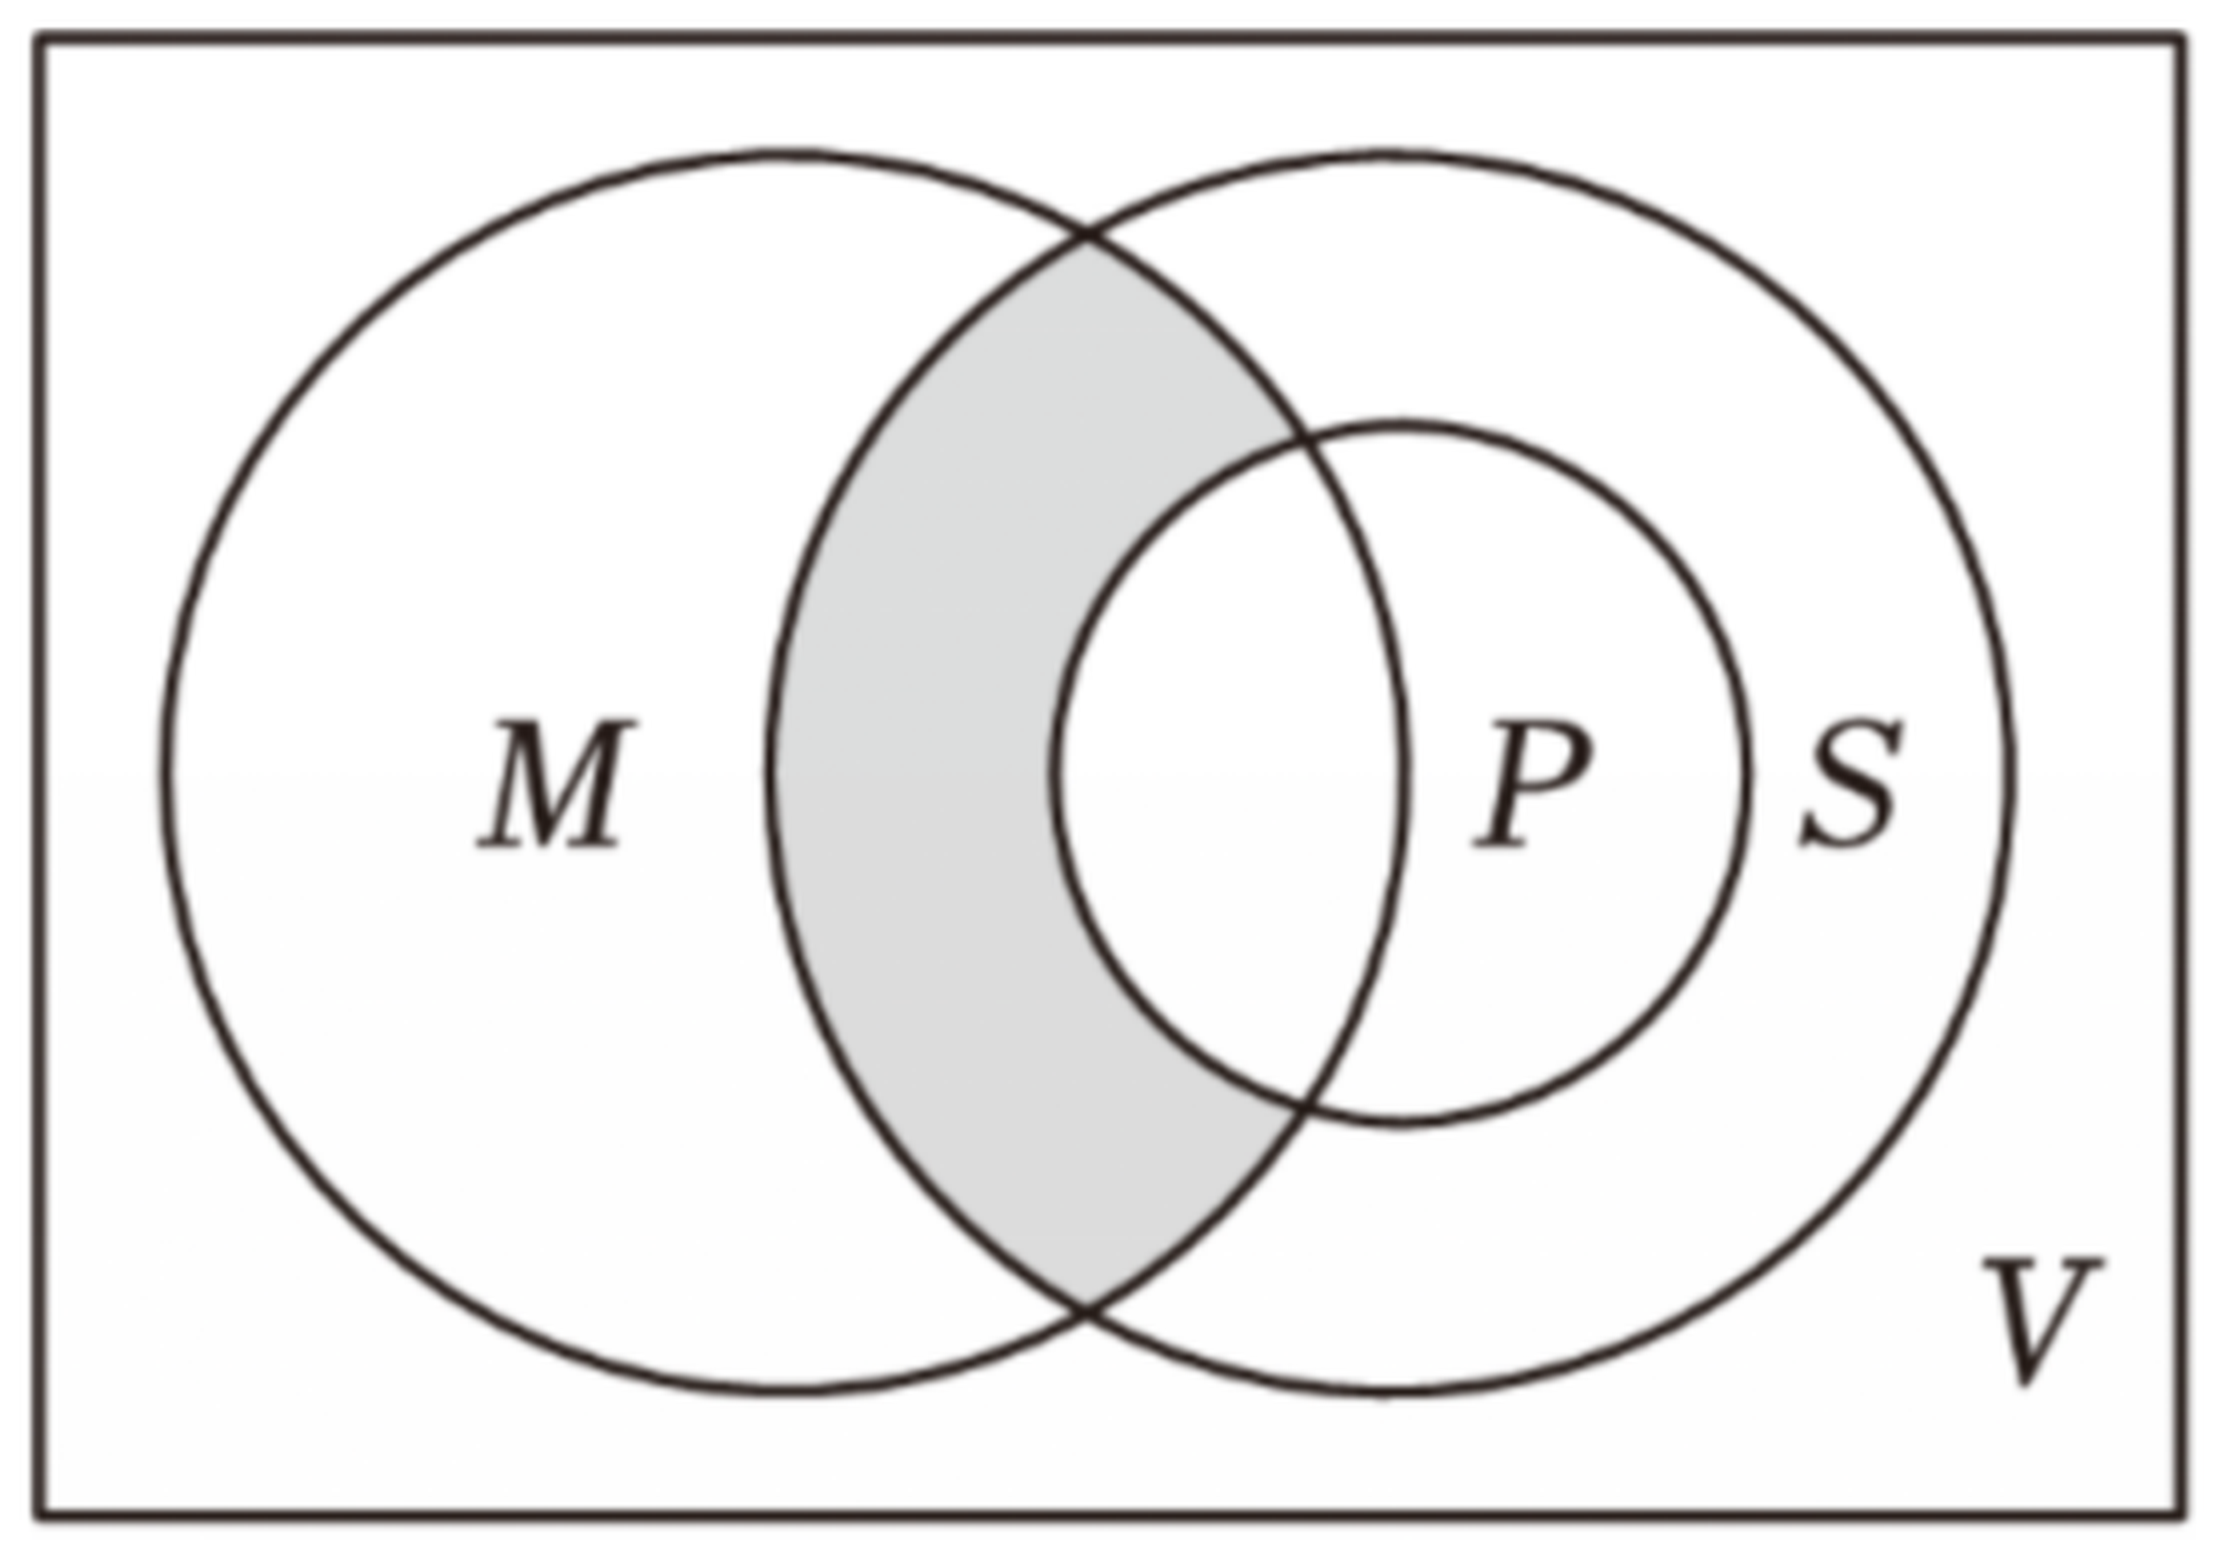
\includegraphics[width=0.38\textwidth]{figures/venn_MPS_V.png}
\end{center}

\ans{$(M\cap S)\cap(\complement_V P)$}

\item 下面六个关系式：① $\varnothing\subseteq\{a\}$；② $a\subseteq\{a\}$；③ $\{a\}\subseteq\{a\}$；④ $\{a\}\in\{a,b\}$；⑤ $a\in\{a,b,c\}$；⑥ $\varnothing\in\{a,b\}$；其中正确的是 \blankline[3.4em].

\ans{①③⑤}

\item 已知集合 $A=\{x\mid -1\le x\le a\}\ne\varnothing$，若 $\{y\mid y=x+1,x\in A\}=\{y\mid y=x^2,x\in A\}$，则实数 $a$ 值为 \blankline[4.4em].

\ans{$0$ 或 $\dfrac{1+\sqrt5}{2}$}

\ifanswer
\solbegin
\step{因为 $A=\{x\mid -1\le x\le a\}\ne\varnothing$，}
\step{所以 $\{y\mid y=x+1,x\in A\}=\{y\mid 0\le y\le a+1\}$，}
\step{$-1\le a\le1$ 时，$\{y\mid y=x^2,x\in A\}=\{y\mid 0\le y\le1\}$，}
\step{$a>1$ 时，$\{y\mid y=x^2,x\in A\}=\{y\mid 0\le y\le a^2\}$，}
\step{① $-1\le a\le1$ 时，$\{y\mid 0\le y\le a+1\}=\{y\mid 0\le y\le1\}$，则 $a+1=1$，解得 $a=0$；}
\step{② $a>1$ 时，$\{y\mid 0\le y\le a+1\}=\{y\mid 0\le y\le a^2\}$，则 $a^2=a+1$，解得 $a=\dfrac{1+\sqrt5}{2}$；}
\step{所以 $a=0$ 或 $\dfrac{1+\sqrt5}{2}$.}
\solend
\fi

\item 设集合 $A=\{(x,y)\mid x+y=22,x>0,y>0,x,y\text{ 均为质数}\}$ 的子集的个数为 \blankline[4.4em].

\ans{$32$}

\ifanswer
\solbegin
\step{集合 $A=\{(x,y)\mid x+y=22,x>0,y>0,x,y\text{ 均为质数}\}$}
\step{$=\{(3,19),(19,3),(5,17),(17,5),(11,11)\}$，则 $A$ 的子集的个数为 $2^5=32$.}
\solend
\fi

% 注：原卷本题题干印作「已知一个有四个数字元素的集合 $S$」；「数字元素」疑为「元素」之衍，
%     但原卷字形确为「数字」二字（已 3× 放大核对过），本稿照录，不代为改写。
\item 已知一个有四个数字元素的集合 $S$，$S$ 的所有子集的元素和（空集的元素和认为是 $0$）的总和为 $16192$，则 $S$ 的元素之和等于 \blankline[4.4em].

\ans{$2024$}

\ifanswer
\solbegin
\step{设 $S=\{a_1,a_2,a_3,a_4\}$，$S$ 的每个元素在所有子集中均出现 $2^3$ 次，}
\step{故 $(a_1+a_2+a_3+a_4)\cdot 2^3=16192$，所以 $a_1+a_2+a_3+a_4=2024$，}
\step{故 $S$ 的元素之和等于 $2024$.}
\solend
\fi

\item 设 $A$ 是非空数集，若对任意 $x$、$y\in A$，都有 $x+y\in A$、$xy\in A$，则称 $A$ 具有性质 $P$，给出以下命题：

①若 $A$ 具有性质 $P$，则 $A$ 可以是有限集；

②若 $A$ 具有性质 $P$，且 $A\ne\R$，则 $\overline A$ 具有性质 $P$；

③若 $A_1$、$A_2$ 具有性质 $P$，且 $A_1\cap A_2\ne\varnothing$，则 $A_1\cap A_2$ 具有性质 $P$；

④若 $A_1$、$A_2$ 具有性质 $P$，则 $A_1\cap A_2$ 具有性质 $P$.

其中所有真命题的序号是 \blankline[4.4em].

\ans{①③}

\ifanswer
\solbegin
\step{对于①，取集合 $A=\{0,1\}$ 具有性质 $P$，故 $A$ 可以是有限集，故①正确；}
\step{对于③，取 $x$、$y\in A_1\cap A_2$，则 $x\in A_1$，$x\in A_2$，$y\in A_1$，$y\in A_2$，}
\step{又 $A_1$、$A_2$ 具有性质 $P$，所以 $x+y\in A_1$，$xy\in A_1$，$x+y\in A_2$，$xy\in A_2$，}
\step{所以 $x+y\in A_1\cap A_2$，$xy\in A_1\cap A_2$，所以 $A_1\cap A_2$ 具有性质 $P$，故③正确；}
\step{对于④，取 $A_1=\{x\mid x=2k,k\in\Z\}$，$A_2=\{x\mid x=3k,k\in\Z\}$，$2\in A_1$，$3\in A_2$，}
\step{但 $2+3\notin A_1\cup A_2$，故④错误；}
\step{对于②，若 $A$ 具有性质 $P$，且 $A\ne\R$，假设 $\overline A$ 也具有性质 $P$，}
\step{设 $0\in A$，在 $\overline A$ 中任取一个 $x$，$x\ne0$，此时可证得 $-x\in A$，}
\step{否则若 $-x\in\overline A$，由于 $\overline A$ 也具有性质 $P$，则 $x+(-x)=0\in\overline A$，}
\step{与 $0\in A$ 矛盾，故 $-x\in A$，}
\step{由于 $A$ 具有性质 $P$，$\overline A$ 也具有性质 $P$，所以 $(-x)^2\in A$，$x^2\in\overline A$，}
\step{而 $(-x)^2=x^2$，这与 $A\cap\overline A=\varnothing$ 矛盾，}
\step{故当 $0\in A$ 且 $A$ 具有性质 $P$ 时，则 $\overline A$ 不具有性质 $P$，}
\step{同理当 $0\in\overline A$ 时，也可以类似推出矛盾，故②错误.}
\step{故正确的是①③.}
\solend
\fi

\item 已知 $S=\{1,2,3,4,5\}$，$A=\{1,2,5\}$，$T=\{t_1,t_2\}\subseteq S$，记 $A_1=\{x\mid x=a+t_1,a\in A,t_1\in T\}$，$A_2=\{x\mid x=b+t_2,b\in A,t_2\in T\}$，若 $A_1\cap A_2=\varnothing$，则集合 $T$ 为 \blankline[5.4em].

\ans{$T=\{1,3\}$ 或 $T=\{2,4\}$ 或 $T=\{3,5\}$}

\ifanswer
\solbegin
\step{若 $A_1\cap A_2=\varnothing$，即 $a+t_1\ne b+t_2$，则 $t_1-t_2\ne a-b$，其中 $a$、$b\in A$，}
\step{否则 $t_1+a=t_2+b$，$A_1\cap A_2\ne\varnothing$，}
\step{又 $S=\{1,2,3,4,5\}$，$A=\{1,2,5\}$，$T=\{t_1,t_2\}\subseteq S$，}
\step{$2-1=1$，$5-2=3$，$5-1=4$，则 $t_1$、$t_2$ 相差 $2$，}
\step{所以 $T=\{1,3\}$ 或 $T=\{2,4\}$ 或 $T=\{3,5\}$.}
\solend
\fi

\end{enumerate}

\bigsec{二、解答题}

\begin{enumerate}
\setcounter{enumi}{13}

\item 设集合 $P=\{1,2,3,m\}$，$Q=\{3,m^2\}$，且 $\overline P\cap Q=\varnothing$，求实数 $m$ 的值组成的集合.

\ans{$\{-1,0,\pm\sqrt2\}$}

\ansspace[5]

\ifanswer
\solbegin
\step{因为 $\overline P\cap Q=\varnothing$，所以 $Q\subseteq P$，所以 $m^2=1$ 或 $m^2=2$ 或 $m^2=m$，}
\step{考虑互异性，得 $m=-1$ 或 $m=\pm\sqrt2$ 或 $m=0$，}
\step{所以实数 $m$ 的值组成的集合为 $\{-1,0,\pm\sqrt2\}$.}
\solend
\fi

\item 若集合 $A=(-\infty,2]$，$B=\{x\mid kx+1<0,k\in\R\}$，$A\cap B=\varnothing$，求实数 $k$ 的取值范围.

\ans{$\left[-\dfrac12,0\right]$}

\ansspace[5]

\ifanswer
\solbegin
\step{若 $B=\varnothing$，则 $k=0$，符合题意，}
\step{若 $B\ne\varnothing$，当 $k>0$ 时，$B=\left(-\infty,-\dfrac1k\right)$，$A\cap B\ne\varnothing$，不合题意；}
\step{当 $k<0$ 时，$B=\left(-\dfrac1k,+\infty\right)$，由 $A\cap B=\varnothing$ 得 $-\dfrac1k\ge2$，即 $-\dfrac12\le k<0$，}
\step{故 $k$ 的取值范围是 $\left[-\dfrac12,0\right]$.}
\solend
\fi

\item 已知集合 $A=\{-4,2a-1,a^2\}$，$B=\{a-5,1-a,9\}$，分别求适合下列条件的 $a$ 的值.

% 两个小问不许与题干分家：试卷版第 2 页页末原本正好把 (1) 留在页底、(2) 翻到次页，
% 与 2026-09-15 修的三类难看切页同源，故在这里也加 \keepwithprev 守卫（三版都生效）。
\keepwithprev
（1）$9\in(A\cap B)$；

\keepwithprev
（2）$\{9\}=A\cap B$.

\ans{（1）$a=5$ 或 $a=-3$；（2）$a=-3$}

\ansspace[5]

\ifanswer
\solbegin
\stepm{（1）}{$9\in(A\cap B)$，所以 $9\in A$，}
\step{当 $2a-1=9$ 时，$a=5$，当 $a^2=9$ 时，即 $a=\pm3$，}
% 注：原卷此句结论印作「所以 $a$ 的值为 $5\backslash-3$」——「\」应是顿号之误，
%     本稿照录原卷字形（见文件头「原卷存疑」②）；按文意即 $a=5$ 或 $a=-3$。
\step{当 $a=3$ 时，$a-5=1-a$ 舍去，所以 $a$ 的值为 $5\backslash-3$.}
\stepm{（2）}{结合（1）的结论：}
\step{当 $2a-1=9$ 即 $a=5$ 时，$1-a=-4$，$\{9\}\ne(A\cap B)$，}
\step{当 $a^2=9$ 时，即 $a=\pm3$，当 $a=3$ 时，$a-5=1-a$ 舍去，}
\step{所以 $a$ 的值为 $-3$.}
\solend
\fi

\item 已知集合 $M=\{a,ab,a-b\}$，$N=\{0,|a|,b\}$，且 $M=N$，求实数 $a$、$b$ 的值.

\ans{$a=b=-1$}

\ansspace[5]

\ifanswer
\solbegin
\step{由集合元素的互异性，得 $a\ne0$，且 $b\ne0$，所以 $a-b=0$，即 $a=b$，}
\step{所以 $ab=|a|$，又由 $|a|\ne b=a$，得 $a<0$，故 $a=b=-1$.}
\solend
\fi

\item 已知集合 $A=\{x\mid -2<x<7\}$，$B=\{x\mid m+1\le x\le 2m-1\}$.

\keepwithprev
（1）当 $m=4$ 时，求 $A\cap B$、$A\cup B$；

\keepwithprev
（2）若 $A\cap B=B$，求实数 $m$ 的取值范围.

\ans{（1）$A\cap B=[5,7)$，$A\cup B=(-2,7]$；（2）$(-\infty,4)$}

\ansspace[5]

\ifanswer
\solbegin
\stepm{（1）}{当 $m=4$ 时，得集合 $A=\{x\mid -2<x<7\}$，$B=\{x\mid 5\le x\le7\}$，}
\step{得 $A\cap B=[5,7)$，$A\cup B=(-2,7]$.}
\stepm{（2）}{由 $A\cap B=B$ 得 $B\subseteq A$，}
\step{①当 $B=\varnothing$ 时，得 $m+1>2m-1$，解得 $m<2$；}
\step{②当 $B\ne\varnothing$ 时，得 $\begin{cases}m+1>-2\\ 2m-1<7\\ m+1\le2m-1\end{cases}$，解得 $2\le m<4$；}
\step{综上，实数 $m$ 的取值范围是 $(-\infty,4)$.}
\solend
\fi

\item 若集合 $A=\{x\mid x^2+5x-6=0\}$，$B=\{x\mid x^2+2(m+1)x+m^2-3=0\}$.

\keepwithprev
（1）当 $m=0$ 时，求集合 $A\cup B$；

\keepwithprev
（2）若 $A\cap B=B$，求实数 $m$ 的取值范围.

\ans{（1）$A\cup B=\{1,-6,-3\}$；（2）$\{m\mid m\le-2\}$}

\ansspace[5]

\ifanswer
\solbegin
\stepm{（1）}{由题意得，集合 $A=\{x\mid x^2+5x-6=0\}=\{1,-6\}$，}
\step{当 $m=0$ 时，$B=\{x\mid x^2+2x-3=0\}=\{1,-3\}$，}
\step{所以 $A\cup B=\{1,-6,-3\}$；}
\stepm{（2）}{由（1）得集合 $A=\{1,-6\}$，$B=\{x\mid x^2+2(m+1)x+m^2-3=0\}$，}
\step{若 $A\cap B=B$ 得 $B\subseteq A$，所以 $B=\varnothing$ 或 $\{-6\}$ 或 $\{1\}$ 或 $\{1,-6\}$，}
\step{当 $B=\varnothing$ 时，$\Delta=4(m+1)^2-4(m^2-3)<0$，解得 $m<-2$，}
\step{当 $B=\{-6\}$ 时，则 $\begin{cases}\Delta=4(m+1)^2-4(m^2-3)=0\\ 36-12(m+1)+m^2-3=0\end{cases}$，无解，}
\step{当 $B=\{1\}$ 时，则 $\begin{cases}\Delta=4(m+1)^2-4(m^2-3)=0\\ 1+2(m+1)+m^2-3=0\end{cases}$，解得 $m=-2$，}
\step{当 $B=\{1,-6\}$ 时，则 $\begin{cases}\Delta=4(m+1)^2-4(m^2-3)>0\\ 1+(-6)=-2(m+1)\\ 1\times(-6)=m^2-3\end{cases}$，无解，}
\step{综上所述，实数 $m$ 的取值范围为 $\{m\mid m\le-2\}$.}
\solend
\fi

% 压轴题：其后已无内容，故作答区全用可丢弃胶水（\ansspace*），并在题目前先量一下版面。
\ansneed{8cm}
\item 对于点集 $A=\{(x,y)\mid x=m,y=-3x+2,m\in\N,m\ge1\}$，$B=\{(x,y)\mid x=n,y=a(x^2-x+1),n\in\N,n\ge1\}$，是否存在非零整数 $a$，使得 $A\cap B\ne\varnothing$？

\ans{$a=-1$}

\ansspace*[10]

\ifanswer
\solbegin
\step{当 $A\cap B\ne\varnothing$ 时，$-3x+2=a(x^2-x+1)$，}
\step{$ax^2+(3-a)x+a-2=0$ ①有正整数解，}
\step{所以 $\Delta=(3-a)^2-4a(a-2)=-3a^2+2a+9$ 是平方数，}
\step{所以 $3a^2-2a-9\le0$，$\dfrac{1-2\sqrt7}{3}\le a\le\dfrac{1+2\sqrt7}{3}$，$a\ne0$，$a\in\Z$，}
\step{所以 $a=\pm1$ 或 $a=2$，}
\step{$a=-1$ 时 $\Delta=4$，这时①变为 $-x^2+4x-3=0$，解得 $x_1=1$，$x_2=3$，}
\step{$A\cap B=\{(1,-1),(3,-7)\}$.}
\step{$a=1$ 时 $\Delta=8$，不是平方数.}
\step{$a=2$ 时 $\Delta=1$，这时①变为 $2x^2+x=0$，没有正整数解.}
\step{所以 $a=-1$.}
\solend
\fi

\end{enumerate}

\end{document}
"
%
% 原始材料是微信公众号图文（公众号「魔都数学加油站」，作者署名「破晓」，
% 原文链接 https://mp.weixin.qq.com/s/tHqWSV1StO5SHSXXQ4jeUA），正文为 6 张 PNG 页；
% 原文本身就是一份**讲评版**——题目下方直接印出【答案】或【解析】。本稿把答案与解析
% 移到答案版，试卷版即一张干净的空卷；试题文字、答案与解析均照原卷录入。
%
% 与原卷的排版差异（均已在 README「说明」中交代）：
%   ① 原文自**第 3 题**起（第 1、2 题未在该文发布），源码里以 \setcounter{enumi}{2} 起编；
%      全卷只有「一、填空题」「二、解答题」两节，无选择题；
%   ② 原卷本就印有两个分节标题（已在原图上逐页放大核对过），本稿照原卷分节，只把标题改排
%      成全稿统一的「大节标题」样式；
%   ③ 原卷的实数集、整数集、自然数集符号作正体 $R$、$Z$、$N$（第 15 题作粗体 $\mathbf{R}$，
%      第 20 题有 $N$ 与斜体 $Z$），本稿按全稿惯例统一写作 $\R$、$\Z$、$\N$；
%   ④ 第 4 题的韦恩图在原卷里印在【解析】右侧（题干并无「如图」二字），故本稿把该图放进
%      答案版的解析块内（`figures/venn_AB_survey_50_x.png`）；第 6、7 题的韦恩图是**题干图**
%      （题干作「图中阴影部分所表示的集合」），两版都排（`figures/venn_A_shaded_U.png`、
%      `figures/venn_MPS_V.png`）。三张图都取自原卷截图、4× LANCZOS 放大，不用 TikZ 手绘；
%   ⑤ 本卷也是「讲评版」，解析按全稿统一的 \solbegin/\step 分步重排（原卷为连续段落），
%      分步不改一字，只断句、断行；
%   ⑥ 标题前缀照**原卷**作「2026--2027 年…」（原卷标题即作「2026-2027年延安中学高一上周末
%      作业 2」）。同校的 高一06 作「学年度」——那是 高一02—高一09 那一批入库时统一改的；
%      后续入库的卷（高一10—高一17 与本卷）一律照原卷保留「年」，未强改，故同校两卷前缀不同。
%
% 原卷存疑两处（已逐处放大到能看清字形后核对，本稿照录并加注，见各题下的 `%` 注）：
%   （另有第三处「第 12 题【解析】末句」原先记作存疑，2026-09-26 第二轮核对放大后发现
%     原卷印的是「$0\in\overline A$」——A 上确有横杠，是本稿当初漏抄了 $\overline{}$；
%     已按原卷补回，故该条从存疑清单里删去，不计为原卷问题。）
%   ① 第 11 题题干印作「已知一个有四个数字元素的集合 $S$」，「数字元素」疑为「元素」之衍；
%   ② 第 16 题 (1) 结论印作「$a$ 的值为 $5\backslash-3$」，其中的「\」应是顿号之误
%      （由 (2) 的结论「$a$ 的值为 $-3$」可反推，(1) 的答案是 $5$ 或 $-3$）；

% 本篇在公众号「魔都数学加油站」连载里的编号是「27学年高一19」，本地编号与之对齐（高一19）；
% 对应关系见 README「与公众号连载号的对照表」。
\documentclass[a4paper,11pt]{article}
\usepackage{common}

\begin{document}

\examtitlest{2026--2027 年延安中学高一上周末作业 2}{集合与常用逻辑用语}

\bigsec{一、填空题}

\begin{enumerate}
% 原卷填空题从第 3 题起（1、2 未在该文中发布），须与解答题的 \setcounter{enumi}{13} 对齐
\setcounter{enumi}{2}
\item 已知全集 $U=\{1,2,3,4,5\}$，$M=\{1,2\}$，$P=\{1,3,5\}$，则 $M\cap\overline P=$ \blankline[4.4em].

\ans{$\{2\}$}

\item 某公司共有 $50$ 人，此次组织参加社会公益活动，其中参加 $A$ 项公益活动的有 $28$ 人，参加 $B$ 项公益活动的有 $33$ 人，且 $A$、$B$ 两项公益活动都不参加的人数比都参加的人数的三分之一多 $1$ 人，则只参加 $A$ 项不参加 $B$ 项的人数是 \blankline[4.4em].

\ans{$10$}

\ifanswer
\solbegin
\step{如图所示，设 $A$、$B$ 两项公益活动都参加的有 $x$ 人，}
\begin{center}
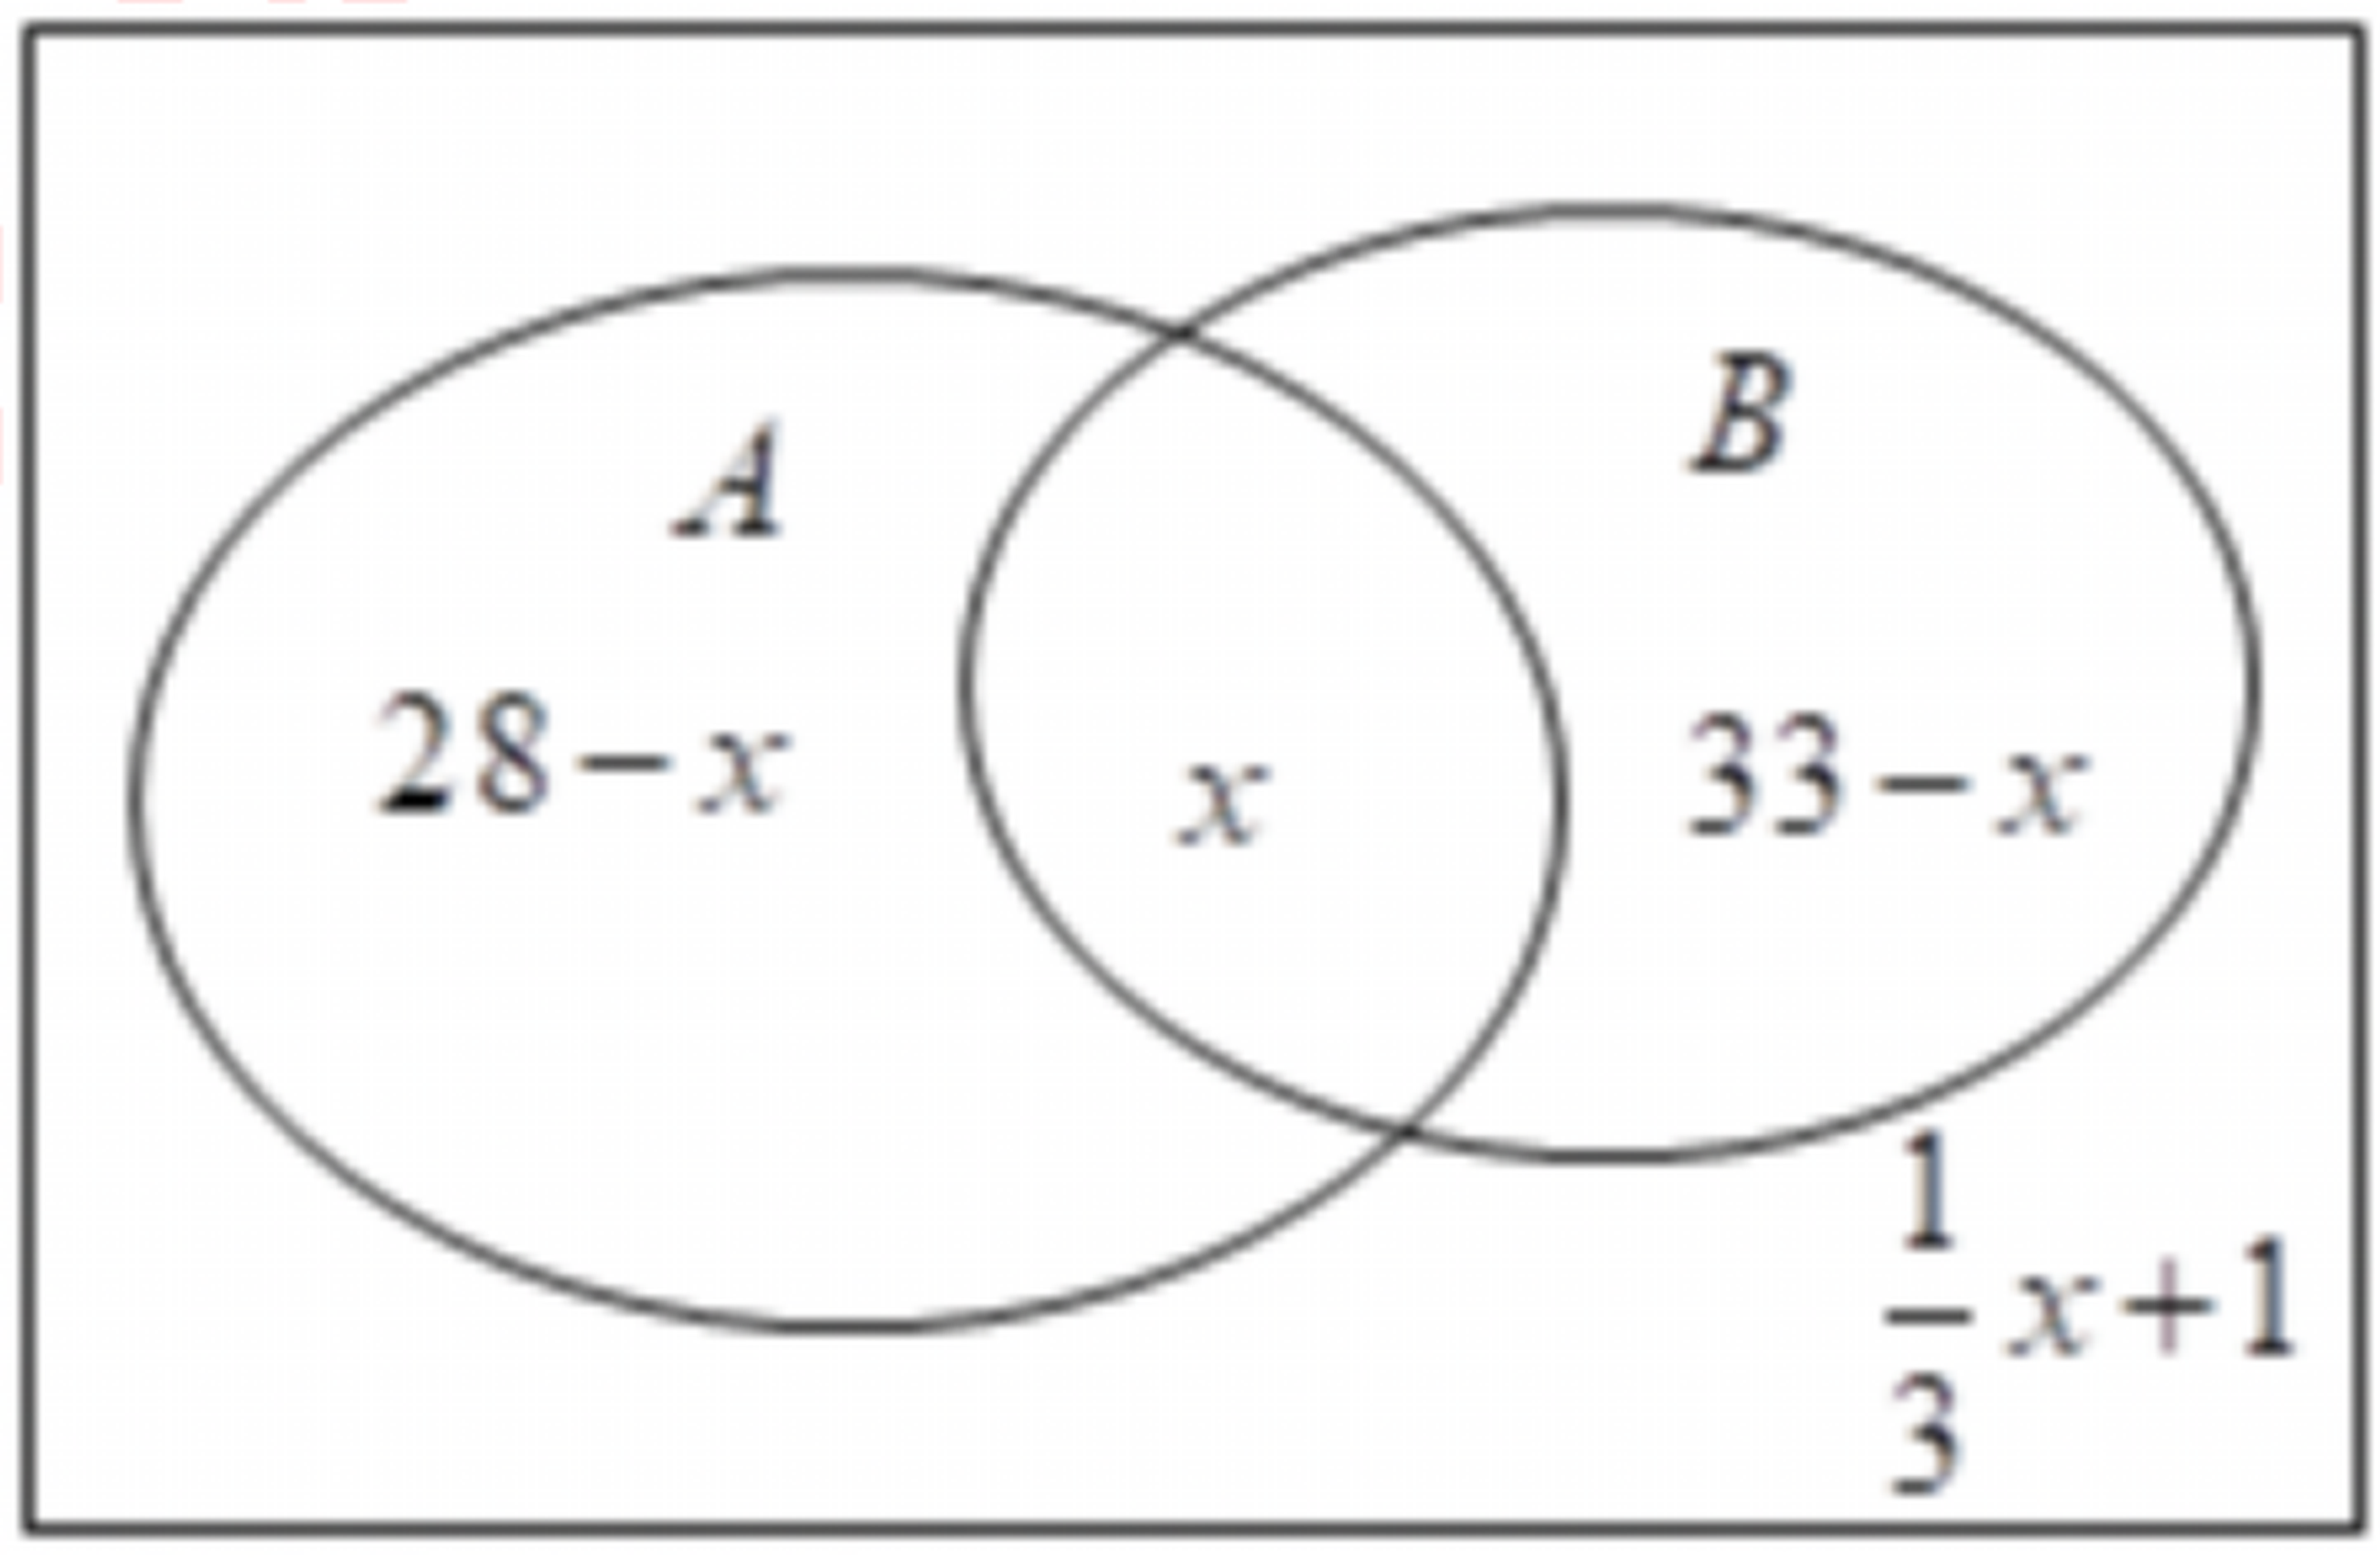
\includegraphics[width=0.42\textwidth]{figures/venn_AB_survey_50_x.png}
\end{center}
\step{则仅参加 $A$ 项的有 $(28-x)$ 人，仅参加 $B$ 项的有 $(33-x)$ 人，}
\step{$A$、$B$ 两项公益活动都不参加的有 $\left(\dfrac13x+1\right)$ 人，}
\step{由题意得 $x+(28-x)+(33-x)+\left(\dfrac13x+1\right)=50$，解得 $x=18$，}
\step{所以只参加 $A$ 项不参加 $B$ 项的有 $28-18=10$ 人.}
\solend
\fi

\item 设集合 $A=\{x\mid x^2-3x+2=0\}$，则满足 $A\cup B=\{0,1,2\}$ 的集合 $B$ 的个数是 \blankline[4.4em].

\ans{$4$}

\ifanswer
\solbegin
\step{$A=\{x\mid x^2-3x+2=0\}=\{x\mid x=1\text{ 或 }x=2\}=\{1,2\}$，}
\step{若 $A\cup B=\{0,1,2\}$，则 $0\in B$，}
\step{则 $B=\{0\},\{0,2\},\{1,0\},\{0,1,2\}$，共 $4$ 个.}
\solend
\fi

\item 已知全集 $U=\R$，集合 $A=\{x\mid x^2<4\}$，$B=\{y\mid y=x^2\}$，则图中阴影部分所表示的集合为 \blankline[4.4em].

\begin{center}
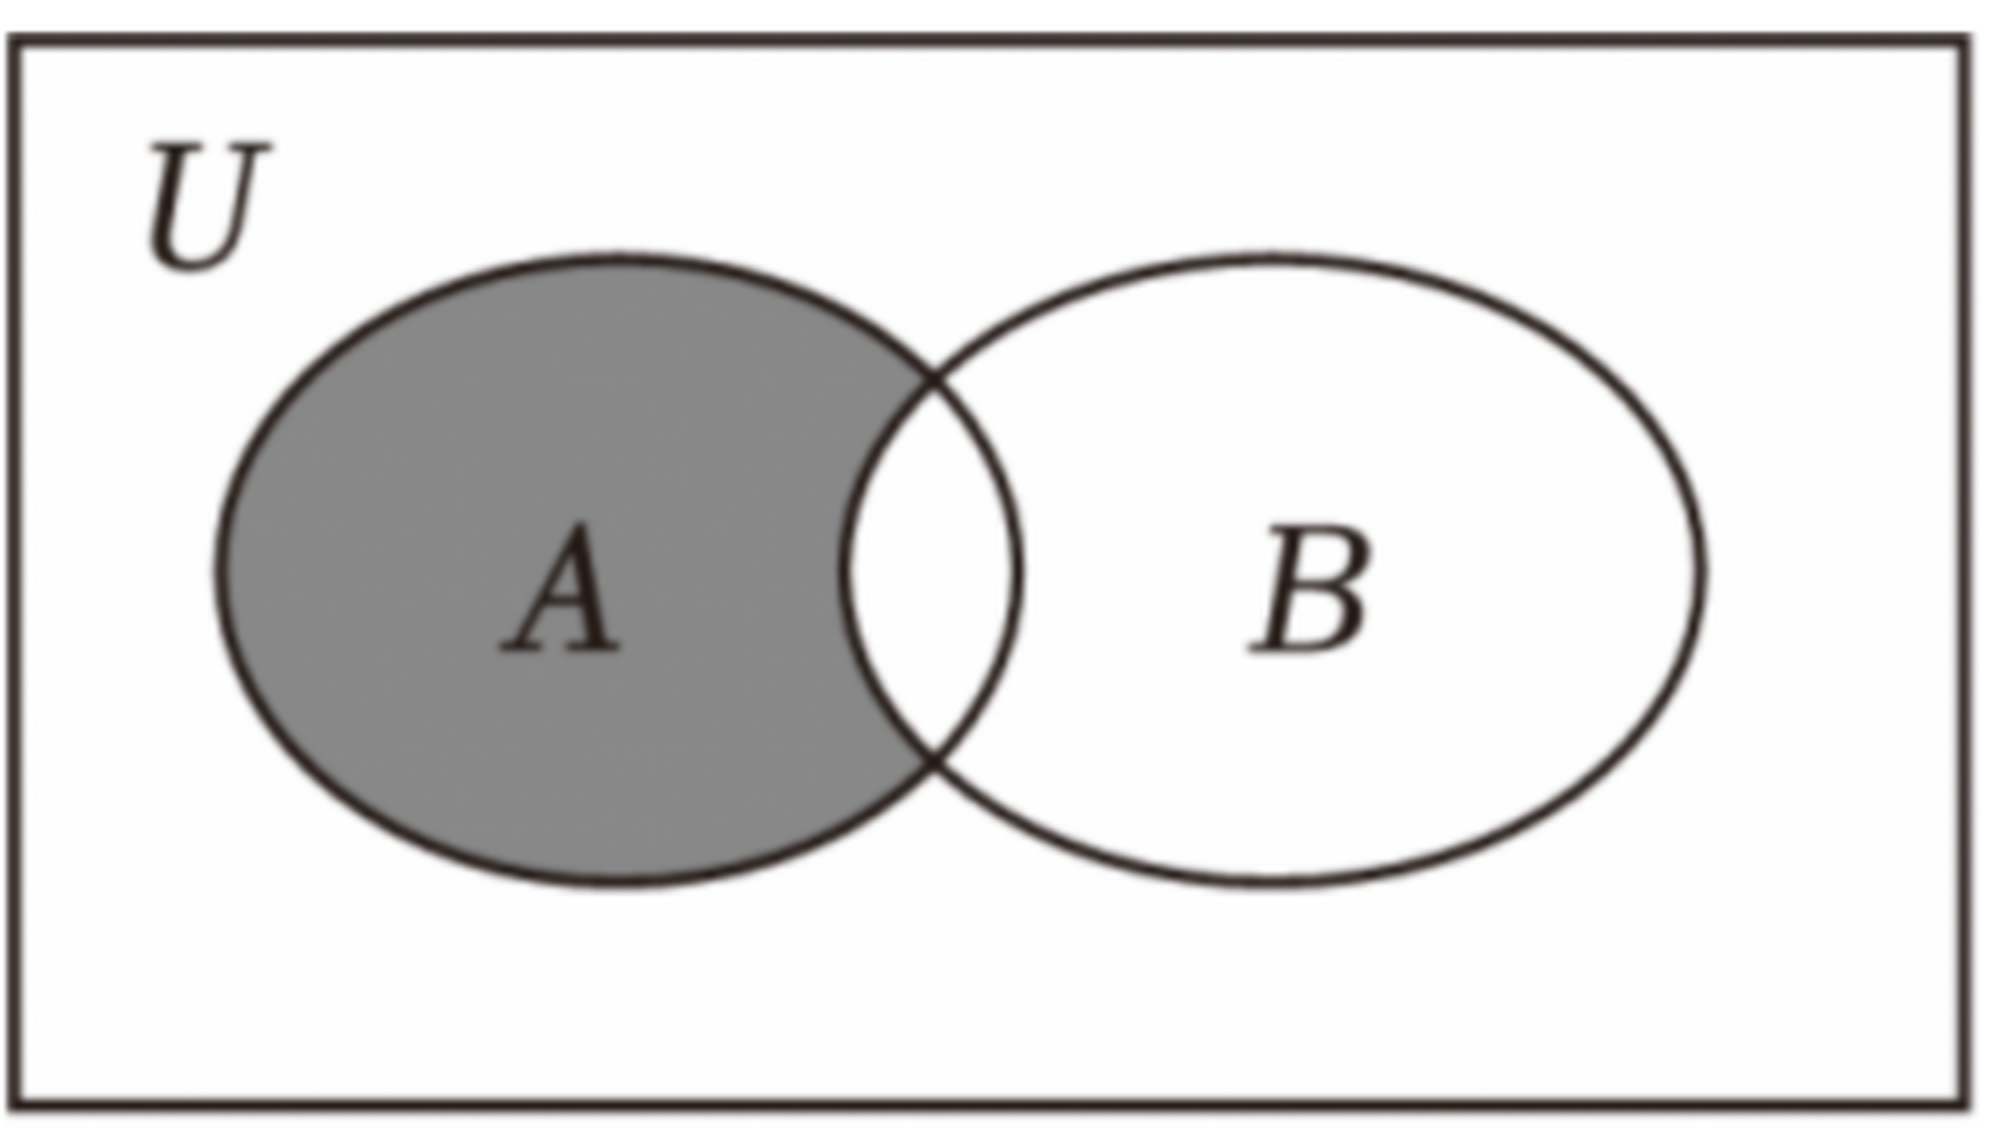
\includegraphics[width=0.34\textwidth]{figures/venn_A_shaded_U.png}
\end{center}

\ans{$A\cap\overline B=(-2,0)$}

\ifanswer
\solbegin
\step{集合 $A=\{x\mid x^2<4\}=(-2,2)$，$B=\{y\mid y=x^2\}=[0,+\infty)$，}
\step{图中阴影部分所表示的集合是 $A\cap\overline B=(-2,0)$.}
\solend
\fi

\item 如图所示，$M$、$P$、$S$ 是 $V$ 的三个子集，则阴影部分所表示的集合是 \blankline[5.4em].

\begin{center}
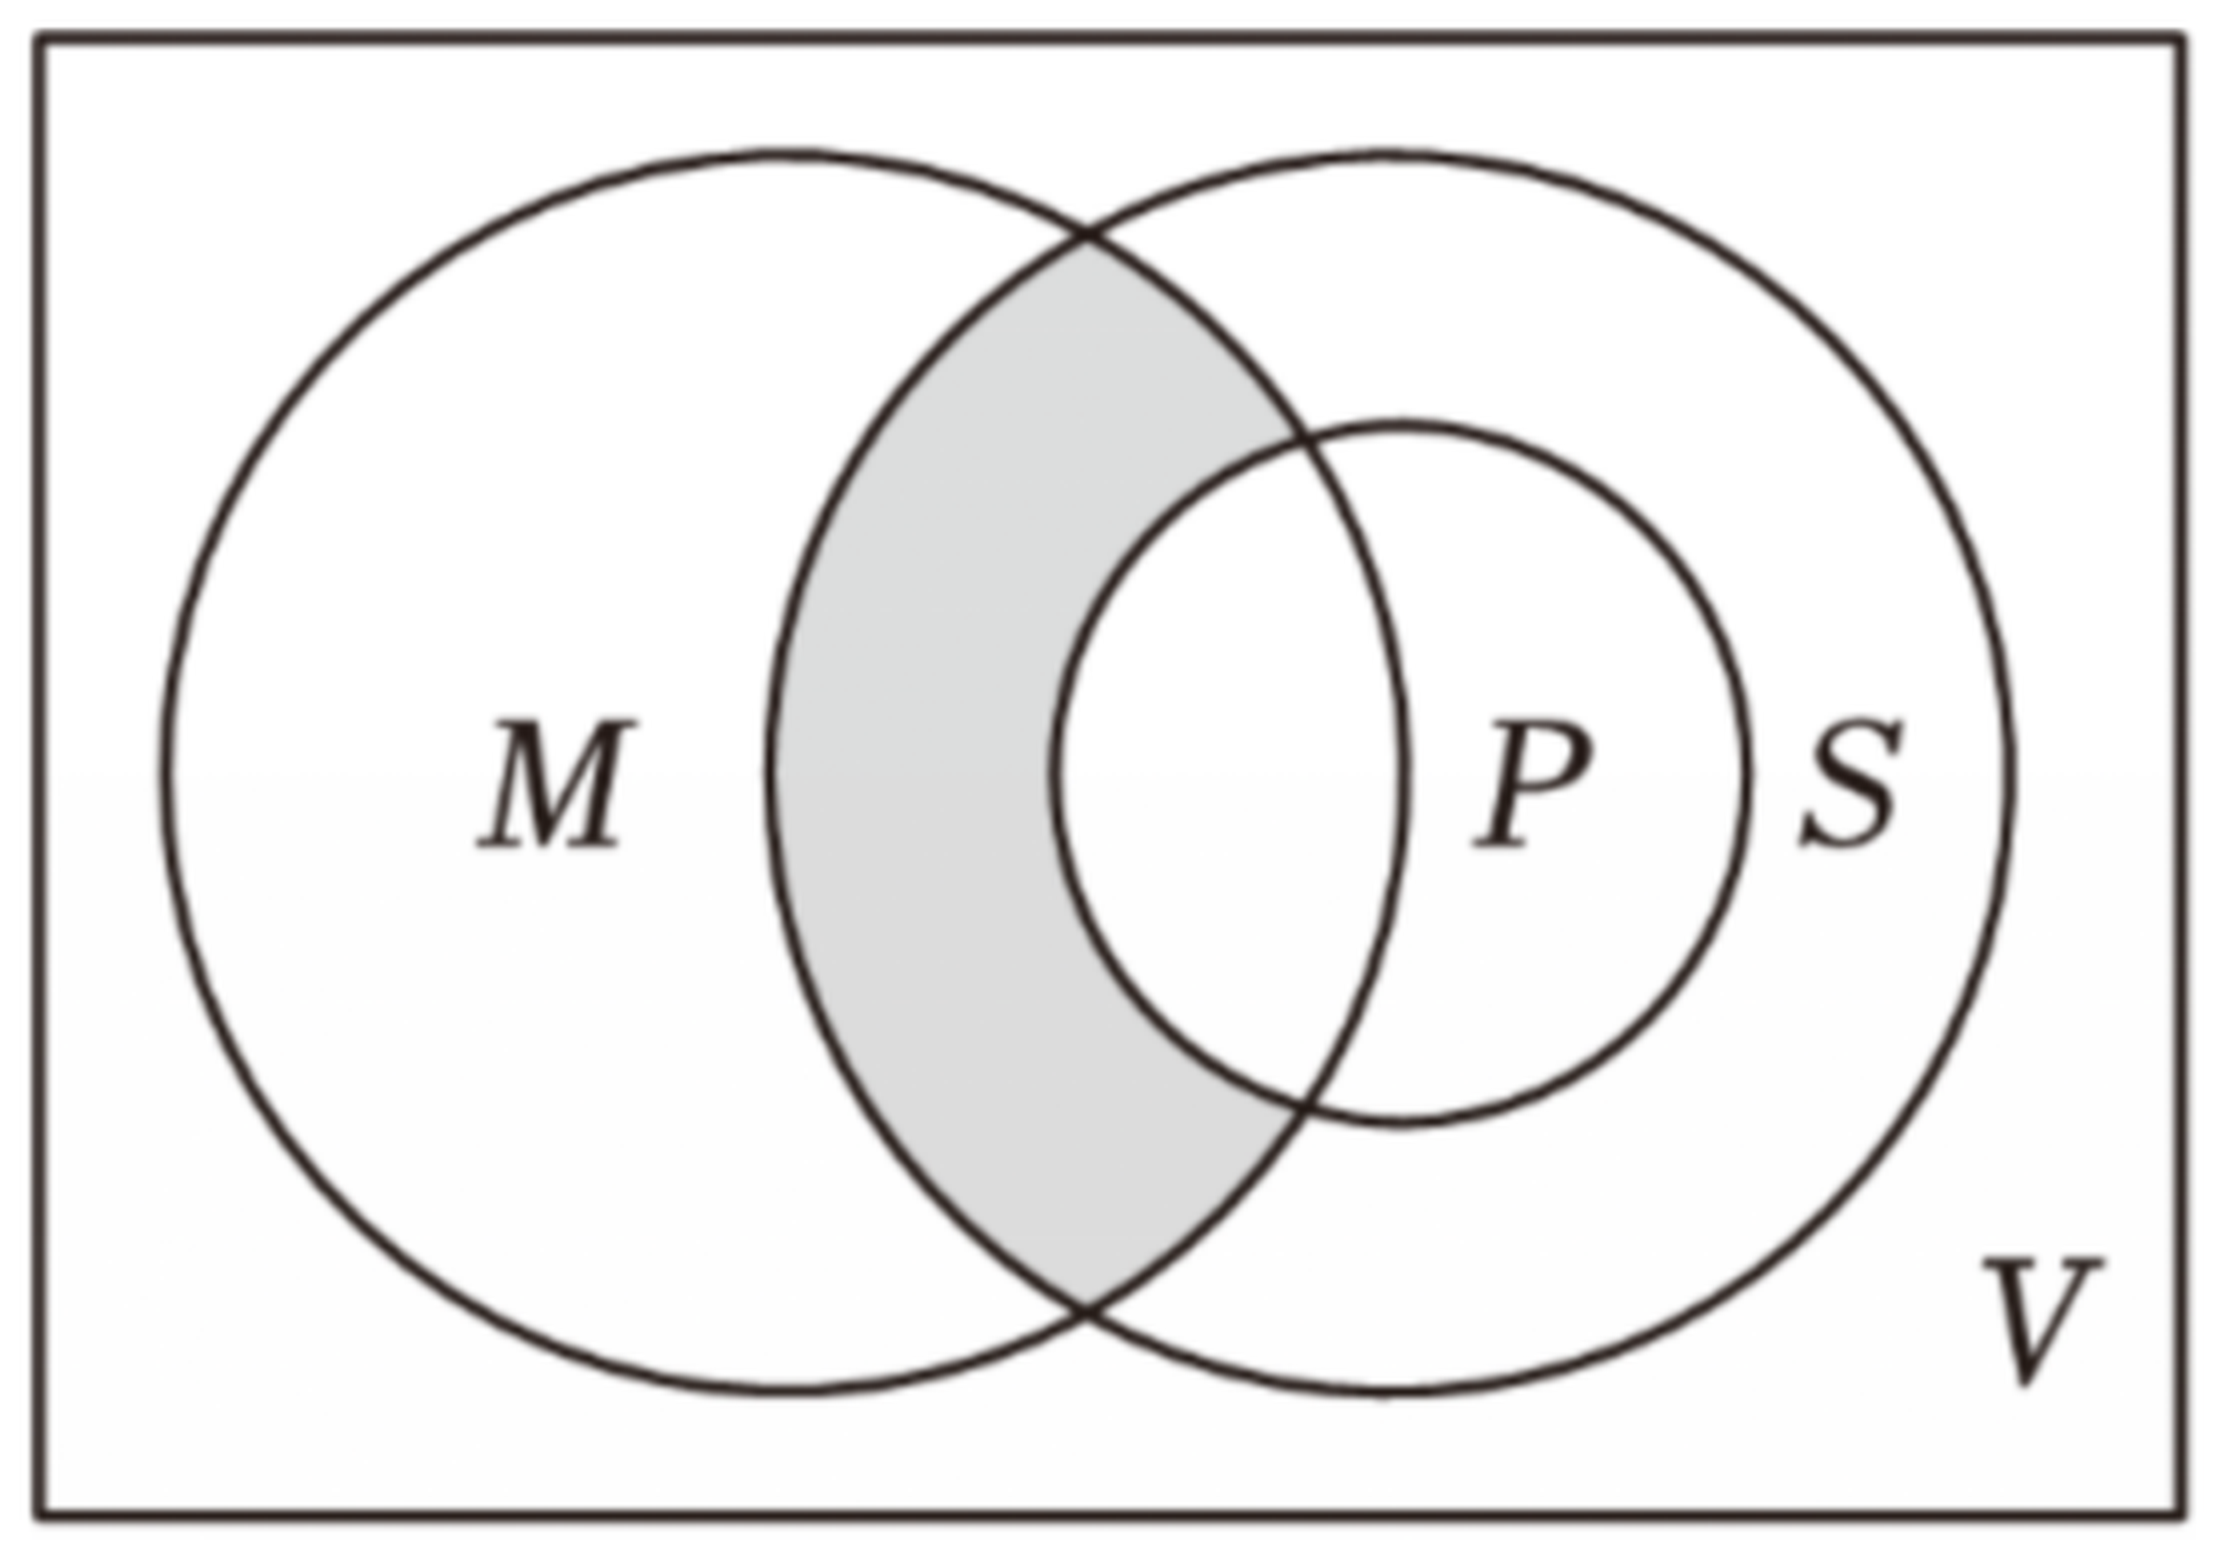
\includegraphics[width=0.38\textwidth]{figures/venn_MPS_V.png}
\end{center}

\ans{$(M\cap S)\cap(\complement_V P)$}

\item 下面六个关系式：① $\varnothing\subseteq\{a\}$；② $a\subseteq\{a\}$；③ $\{a\}\subseteq\{a\}$；④ $\{a\}\in\{a,b\}$；⑤ $a\in\{a,b,c\}$；⑥ $\varnothing\in\{a,b\}$；其中正确的是 \blankline[3.4em].

\ans{①③⑤}

\item 已知集合 $A=\{x\mid -1\le x\le a\}\ne\varnothing$，若 $\{y\mid y=x+1,x\in A\}=\{y\mid y=x^2,x\in A\}$，则实数 $a$ 值为 \blankline[4.4em].

\ans{$0$ 或 $\dfrac{1+\sqrt5}{2}$}

\ifanswer
\solbegin
\step{因为 $A=\{x\mid -1\le x\le a\}\ne\varnothing$，}
\step{所以 $\{y\mid y=x+1,x\in A\}=\{y\mid 0\le y\le a+1\}$，}
\step{$-1\le a\le1$ 时，$\{y\mid y=x^2,x\in A\}=\{y\mid 0\le y\le1\}$，}
\step{$a>1$ 时，$\{y\mid y=x^2,x\in A\}=\{y\mid 0\le y\le a^2\}$，}
\step{① $-1\le a\le1$ 时，$\{y\mid 0\le y\le a+1\}=\{y\mid 0\le y\le1\}$，则 $a+1=1$，解得 $a=0$；}
\step{② $a>1$ 时，$\{y\mid 0\le y\le a+1\}=\{y\mid 0\le y\le a^2\}$，则 $a^2=a+1$，解得 $a=\dfrac{1+\sqrt5}{2}$；}
\step{所以 $a=0$ 或 $\dfrac{1+\sqrt5}{2}$.}
\solend
\fi

\item 设集合 $A=\{(x,y)\mid x+y=22,x>0,y>0,x,y\text{ 均为质数}\}$ 的子集的个数为 \blankline[4.4em].

\ans{$32$}

\ifanswer
\solbegin
\step{集合 $A=\{(x,y)\mid x+y=22,x>0,y>0,x,y\text{ 均为质数}\}$}
\step{$=\{(3,19),(19,3),(5,17),(17,5),(11,11)\}$，则 $A$ 的子集的个数为 $2^5=32$.}
\solend
\fi

% 注：原卷本题题干印作「已知一个有四个数字元素的集合 $S$」；「数字元素」疑为「元素」之衍，
%     但原卷字形确为「数字」二字（已 3× 放大核对过），本稿照录，不代为改写。
\item 已知一个有四个数字元素的集合 $S$，$S$ 的所有子集的元素和（空集的元素和认为是 $0$）的总和为 $16192$，则 $S$ 的元素之和等于 \blankline[4.4em].

\ans{$2024$}

\ifanswer
\solbegin
\step{设 $S=\{a_1,a_2,a_3,a_4\}$，$S$ 的每个元素在所有子集中均出现 $2^3$ 次，}
\step{故 $(a_1+a_2+a_3+a_4)\cdot 2^3=16192$，所以 $a_1+a_2+a_3+a_4=2024$，}
\step{故 $S$ 的元素之和等于 $2024$.}
\solend
\fi

\item 设 $A$ 是非空数集，若对任意 $x$、$y\in A$，都有 $x+y\in A$、$xy\in A$，则称 $A$ 具有性质 $P$，给出以下命题：

①若 $A$ 具有性质 $P$，则 $A$ 可以是有限集；

②若 $A$ 具有性质 $P$，且 $A\ne\R$，则 $\overline A$ 具有性质 $P$；

③若 $A_1$、$A_2$ 具有性质 $P$，且 $A_1\cap A_2\ne\varnothing$，则 $A_1\cap A_2$ 具有性质 $P$；

④若 $A_1$、$A_2$ 具有性质 $P$，则 $A_1\cap A_2$ 具有性质 $P$.

其中所有真命题的序号是 \blankline[4.4em].

\ans{①③}

\ifanswer
\solbegin
\step{对于①，取集合 $A=\{0,1\}$ 具有性质 $P$，故 $A$ 可以是有限集，故①正确；}
\step{对于③，取 $x$、$y\in A_1\cap A_2$，则 $x\in A_1$，$x\in A_2$，$y\in A_1$，$y\in A_2$，}
\step{又 $A_1$、$A_2$ 具有性质 $P$，所以 $x+y\in A_1$，$xy\in A_1$，$x+y\in A_2$，$xy\in A_2$，}
\step{所以 $x+y\in A_1\cap A_2$，$xy\in A_1\cap A_2$，所以 $A_1\cap A_2$ 具有性质 $P$，故③正确；}
\step{对于④，取 $A_1=\{x\mid x=2k,k\in\Z\}$，$A_2=\{x\mid x=3k,k\in\Z\}$，$2\in A_1$，$3\in A_2$，}
\step{但 $2+3\notin A_1\cup A_2$，故④错误；}
\step{对于②，若 $A$ 具有性质 $P$，且 $A\ne\R$，假设 $\overline A$ 也具有性质 $P$，}
\step{设 $0\in A$，在 $\overline A$ 中任取一个 $x$，$x\ne0$，此时可证得 $-x\in A$，}
\step{否则若 $-x\in\overline A$，由于 $\overline A$ 也具有性质 $P$，则 $x+(-x)=0\in\overline A$，}
\step{与 $0\in A$ 矛盾，故 $-x\in A$，}
\step{由于 $A$ 具有性质 $P$，$\overline A$ 也具有性质 $P$，所以 $(-x)^2\in A$，$x^2\in\overline A$，}
\step{而 $(-x)^2=x^2$，这与 $A\cap\overline A=\varnothing$ 矛盾，}
\step{故当 $0\in A$ 且 $A$ 具有性质 $P$ 时，则 $\overline A$ 不具有性质 $P$，}
\step{同理当 $0\in\overline A$ 时，也可以类似推出矛盾，故②错误.}
\step{故正确的是①③.}
\solend
\fi

\item 已知 $S=\{1,2,3,4,5\}$，$A=\{1,2,5\}$，$T=\{t_1,t_2\}\subseteq S$，记 $A_1=\{x\mid x=a+t_1,a\in A,t_1\in T\}$，$A_2=\{x\mid x=b+t_2,b\in A,t_2\in T\}$，若 $A_1\cap A_2=\varnothing$，则集合 $T$ 为 \blankline[5.4em].

\ans{$T=\{1,3\}$ 或 $T=\{2,4\}$ 或 $T=\{3,5\}$}

\ifanswer
\solbegin
\step{若 $A_1\cap A_2=\varnothing$，即 $a+t_1\ne b+t_2$，则 $t_1-t_2\ne a-b$，其中 $a$、$b\in A$，}
\step{否则 $t_1+a=t_2+b$，$A_1\cap A_2\ne\varnothing$，}
\step{又 $S=\{1,2,3,4,5\}$，$A=\{1,2,5\}$，$T=\{t_1,t_2\}\subseteq S$，}
\step{$2-1=1$，$5-2=3$，$5-1=4$，则 $t_1$、$t_2$ 相差 $2$，}
\step{所以 $T=\{1,3\}$ 或 $T=\{2,4\}$ 或 $T=\{3,5\}$.}
\solend
\fi

\end{enumerate}

\bigsec{二、解答题}

\begin{enumerate}
\setcounter{enumi}{13}

\item 设集合 $P=\{1,2,3,m\}$，$Q=\{3,m^2\}$，且 $\overline P\cap Q=\varnothing$，求实数 $m$ 的值组成的集合.

\ans{$\{-1,0,\pm\sqrt2\}$}

\ansspace[5]

\ifanswer
\solbegin
\step{因为 $\overline P\cap Q=\varnothing$，所以 $Q\subseteq P$，所以 $m^2=1$ 或 $m^2=2$ 或 $m^2=m$，}
\step{考虑互异性，得 $m=-1$ 或 $m=\pm\sqrt2$ 或 $m=0$，}
\step{所以实数 $m$ 的值组成的集合为 $\{-1,0,\pm\sqrt2\}$.}
\solend
\fi

\item 若集合 $A=(-\infty,2]$，$B=\{x\mid kx+1<0,k\in\R\}$，$A\cap B=\varnothing$，求实数 $k$ 的取值范围.

\ans{$\left[-\dfrac12,0\right]$}

\ansspace[5]

\ifanswer
\solbegin
\step{若 $B=\varnothing$，则 $k=0$，符合题意，}
\step{若 $B\ne\varnothing$，当 $k>0$ 时，$B=\left(-\infty,-\dfrac1k\right)$，$A\cap B\ne\varnothing$，不合题意；}
\step{当 $k<0$ 时，$B=\left(-\dfrac1k,+\infty\right)$，由 $A\cap B=\varnothing$ 得 $-\dfrac1k\ge2$，即 $-\dfrac12\le k<0$，}
\step{故 $k$ 的取值范围是 $\left[-\dfrac12,0\right]$.}
\solend
\fi

\item 已知集合 $A=\{-4,2a-1,a^2\}$，$B=\{a-5,1-a,9\}$，分别求适合下列条件的 $a$ 的值.

% 两个小问不许与题干分家：试卷版第 2 页页末原本正好把 (1) 留在页底、(2) 翻到次页，
% 与 2026-09-15 修的三类难看切页同源，故在这里也加 \keepwithprev 守卫（三版都生效）。
\keepwithprev
（1）$9\in(A\cap B)$；

\keepwithprev
（2）$\{9\}=A\cap B$.

\ans{（1）$a=5$ 或 $a=-3$；（2）$a=-3$}

\ansspace[5]

\ifanswer
\solbegin
\stepm{（1）}{$9\in(A\cap B)$，所以 $9\in A$，}
\step{当 $2a-1=9$ 时，$a=5$，当 $a^2=9$ 时，即 $a=\pm3$，}
% 注：原卷此句结论印作「所以 $a$ 的值为 $5\backslash-3$」——「\」应是顿号之误，
%     本稿照录原卷字形（见文件头「原卷存疑」②）；按文意即 $a=5$ 或 $a=-3$。
\step{当 $a=3$ 时，$a-5=1-a$ 舍去，所以 $a$ 的值为 $5\backslash-3$.}
\stepm{（2）}{结合（1）的结论：}
\step{当 $2a-1=9$ 即 $a=5$ 时，$1-a=-4$，$\{9\}\ne(A\cap B)$，}
\step{当 $a^2=9$ 时，即 $a=\pm3$，当 $a=3$ 时，$a-5=1-a$ 舍去，}
\step{所以 $a$ 的值为 $-3$.}
\solend
\fi

\item 已知集合 $M=\{a,ab,a-b\}$，$N=\{0,|a|,b\}$，且 $M=N$，求实数 $a$、$b$ 的值.

\ans{$a=b=-1$}

\ansspace[5]

\ifanswer
\solbegin
\step{由集合元素的互异性，得 $a\ne0$，且 $b\ne0$，所以 $a-b=0$，即 $a=b$，}
\step{所以 $ab=|a|$，又由 $|a|\ne b=a$，得 $a<0$，故 $a=b=-1$.}
\solend
\fi

\item 已知集合 $A=\{x\mid -2<x<7\}$，$B=\{x\mid m+1\le x\le 2m-1\}$.

\keepwithprev
（1）当 $m=4$ 时，求 $A\cap B$、$A\cup B$；

\keepwithprev
（2）若 $A\cap B=B$，求实数 $m$ 的取值范围.

\ans{（1）$A\cap B=[5,7)$，$A\cup B=(-2,7]$；（2）$(-\infty,4)$}

\ansspace[5]

\ifanswer
\solbegin
\stepm{（1）}{当 $m=4$ 时，得集合 $A=\{x\mid -2<x<7\}$，$B=\{x\mid 5\le x\le7\}$，}
\step{得 $A\cap B=[5,7)$，$A\cup B=(-2,7]$.}
\stepm{（2）}{由 $A\cap B=B$ 得 $B\subseteq A$，}
\step{①当 $B=\varnothing$ 时，得 $m+1>2m-1$，解得 $m<2$；}
\step{②当 $B\ne\varnothing$ 时，得 $\begin{cases}m+1>-2\\ 2m-1<7\\ m+1\le2m-1\end{cases}$，解得 $2\le m<4$；}
\step{综上，实数 $m$ 的取值范围是 $(-\infty,4)$.}
\solend
\fi

\item 若集合 $A=\{x\mid x^2+5x-6=0\}$，$B=\{x\mid x^2+2(m+1)x+m^2-3=0\}$.

\keepwithprev
（1）当 $m=0$ 时，求集合 $A\cup B$；

\keepwithprev
（2）若 $A\cap B=B$，求实数 $m$ 的取值范围.

\ans{（1）$A\cup B=\{1,-6,-3\}$；（2）$\{m\mid m\le-2\}$}

\ansspace[5]

\ifanswer
\solbegin
\stepm{（1）}{由题意得，集合 $A=\{x\mid x^2+5x-6=0\}=\{1,-6\}$，}
\step{当 $m=0$ 时，$B=\{x\mid x^2+2x-3=0\}=\{1,-3\}$，}
\step{所以 $A\cup B=\{1,-6,-3\}$；}
\stepm{（2）}{由（1）得集合 $A=\{1,-6\}$，$B=\{x\mid x^2+2(m+1)x+m^2-3=0\}$，}
\step{若 $A\cap B=B$ 得 $B\subseteq A$，所以 $B=\varnothing$ 或 $\{-6\}$ 或 $\{1\}$ 或 $\{1,-6\}$，}
\step{当 $B=\varnothing$ 时，$\Delta=4(m+1)^2-4(m^2-3)<0$，解得 $m<-2$，}
\step{当 $B=\{-6\}$ 时，则 $\begin{cases}\Delta=4(m+1)^2-4(m^2-3)=0\\ 36-12(m+1)+m^2-3=0\end{cases}$，无解，}
\step{当 $B=\{1\}$ 时，则 $\begin{cases}\Delta=4(m+1)^2-4(m^2-3)=0\\ 1+2(m+1)+m^2-3=0\end{cases}$，解得 $m=-2$，}
\step{当 $B=\{1,-6\}$ 时，则 $\begin{cases}\Delta=4(m+1)^2-4(m^2-3)>0\\ 1+(-6)=-2(m+1)\\ 1\times(-6)=m^2-3\end{cases}$，无解，}
\step{综上所述，实数 $m$ 的取值范围为 $\{m\mid m\le-2\}$.}
\solend
\fi

% 压轴题：其后已无内容，故作答区全用可丢弃胶水（\ansspace*），并在题目前先量一下版面。
\ansneed{8cm}
\item 对于点集 $A=\{(x,y)\mid x=m,y=-3x+2,m\in\N,m\ge1\}$，$B=\{(x,y)\mid x=n,y=a(x^2-x+1),n\in\N,n\ge1\}$，是否存在非零整数 $a$，使得 $A\cap B\ne\varnothing$？

\ans{$a=-1$}

\ansspace*[10]

\ifanswer
\solbegin
\step{当 $A\cap B\ne\varnothing$ 时，$-3x+2=a(x^2-x+1)$，}
\step{$ax^2+(3-a)x+a-2=0$ ①有正整数解，}
\step{所以 $\Delta=(3-a)^2-4a(a-2)=-3a^2+2a+9$ 是平方数，}
\step{所以 $3a^2-2a-9\le0$，$\dfrac{1-2\sqrt7}{3}\le a\le\dfrac{1+2\sqrt7}{3}$，$a\ne0$，$a\in\Z$，}
\step{所以 $a=\pm1$ 或 $a=2$，}
\step{$a=-1$ 时 $\Delta=4$，这时①变为 $-x^2+4x-3=0$，解得 $x_1=1$，$x_2=3$，}
\step{$A\cap B=\{(1,-1),(3,-7)\}$.}
\step{$a=1$ 时 $\Delta=8$，不是平方数.}
\step{$a=2$ 时 $\Delta=1$，这时①变为 $2x^2+x=0$，没有正整数解.}
\step{所以 $a=-1$.}
\solend
\fi

\end{enumerate}

\end{document}
"
%
% 原始材料是微信公众号图文（公众号「魔都数学加油站」，作者署名「破晓」，
% 原文链接 https://mp.weixin.qq.com/s/tHqWSV1StO5SHSXXQ4jeUA），正文为 6 张 PNG 页；
% 原文本身就是一份**讲评版**——题目下方直接印出【答案】或【解析】。本稿把答案与解析
% 移到答案版，试卷版即一张干净的空卷；试题文字、答案与解析均照原卷录入。
%
% 与原卷的排版差异（均已在 README「说明」中交代）：
%   ① 原文自**第 3 题**起（第 1、2 题未在该文发布），源码里以 \setcounter{enumi}{2} 起编；
%      全卷只有「一、填空题」「二、解答题」两节，无选择题；
%   ② 原卷本就印有两个分节标题（已在原图上逐页放大核对过），本稿照原卷分节，只把标题改排
%      成全稿统一的「大节标题」样式；
%   ③ 原卷的实数集、整数集、自然数集符号作正体 $R$、$Z$、$N$（第 15 题作粗体 $\mathbf{R}$，
%      第 20 题有 $N$ 与斜体 $Z$），本稿按全稿惯例统一写作 $\R$、$\Z$、$\N$；
%   ④ 第 4 题的韦恩图在原卷里印在【解析】右侧（题干并无「如图」二字），故本稿把该图放进
%      答案版的解析块内（`figures/venn_AB_survey_50_x.png`）；第 6、7 题的韦恩图是**题干图**
%      （题干作「图中阴影部分所表示的集合」），两版都排（`figures/venn_A_shaded_U.png`、
%      `figures/venn_MPS_V.png`）。三张图都取自原卷截图、4× LANCZOS 放大，不用 TikZ 手绘；
%   ⑤ 本卷也是「讲评版」，解析按全稿统一的 \solbegin/\step 分步重排（原卷为连续段落），
%      分步不改一字，只断句、断行；
%   ⑥ 标题前缀照**原卷**作「2026--2027 年…」（原卷标题即作「2026-2027年延安中学高一上周末
%      作业 2」）。同校的 高一06 作「学年度」——那是 高一02—高一09 那一批入库时统一改的；
%      后续入库的卷（高一10—高一17 与本卷）一律照原卷保留「年」，未强改，故同校两卷前缀不同。
%
% 原卷存疑两处（已逐处放大到能看清字形后核对，本稿照录并加注，见各题下的 `%` 注）：
%   （另有第三处「第 12 题【解析】末句」原先记作存疑，2026-09-26 第二轮核对放大后发现
%     原卷印的是「$0\in\overline A$」——A 上确有横杠，是本稿当初漏抄了 $\overline{}$；
%     已按原卷补回，故该条从存疑清单里删去，不计为原卷问题。）
%   ① 第 11 题题干印作「已知一个有四个数字元素的集合 $S$」，「数字元素」疑为「元素」之衍；
%   ② 第 16 题 (1) 结论印作「$a$ 的值为 $5\backslash-3$」，其中的「\」应是顿号之误
%      （由 (2) 的结论「$a$ 的值为 $-3$」可反推，(1) 的答案是 $5$ 或 $-3$）；

% 本篇在公众号「魔都数学加油站」连载里的编号是「27学年高一19」，本地编号与之对齐（高一19）；
% 对应关系见 README「与公众号连载号的对照表」。
\documentclass[a4paper,11pt]{article}
\usepackage{common}

\begin{document}

\examtitlest{2026--2027 年延安中学高一上周末作业 2}{集合与常用逻辑用语}

\bigsec{一、填空题}

\begin{enumerate}
% 原卷填空题从第 3 题起（1、2 未在该文中发布），须与解答题的 \setcounter{enumi}{13} 对齐
\setcounter{enumi}{2}
\item 已知全集 $U=\{1,2,3,4,5\}$，$M=\{1,2\}$，$P=\{1,3,5\}$，则 $M\cap\overline P=$ \blankline[4.4em].

\ans{$\{2\}$}

\item 某公司共有 $50$ 人，此次组织参加社会公益活动，其中参加 $A$ 项公益活动的有 $28$ 人，参加 $B$ 项公益活动的有 $33$ 人，且 $A$、$B$ 两项公益活动都不参加的人数比都参加的人数的三分之一多 $1$ 人，则只参加 $A$ 项不参加 $B$ 项的人数是 \blankline[4.4em].

\ans{$10$}

\ifanswer
\solbegin
\step{如图所示，设 $A$、$B$ 两项公益活动都参加的有 $x$ 人，}
\begin{center}
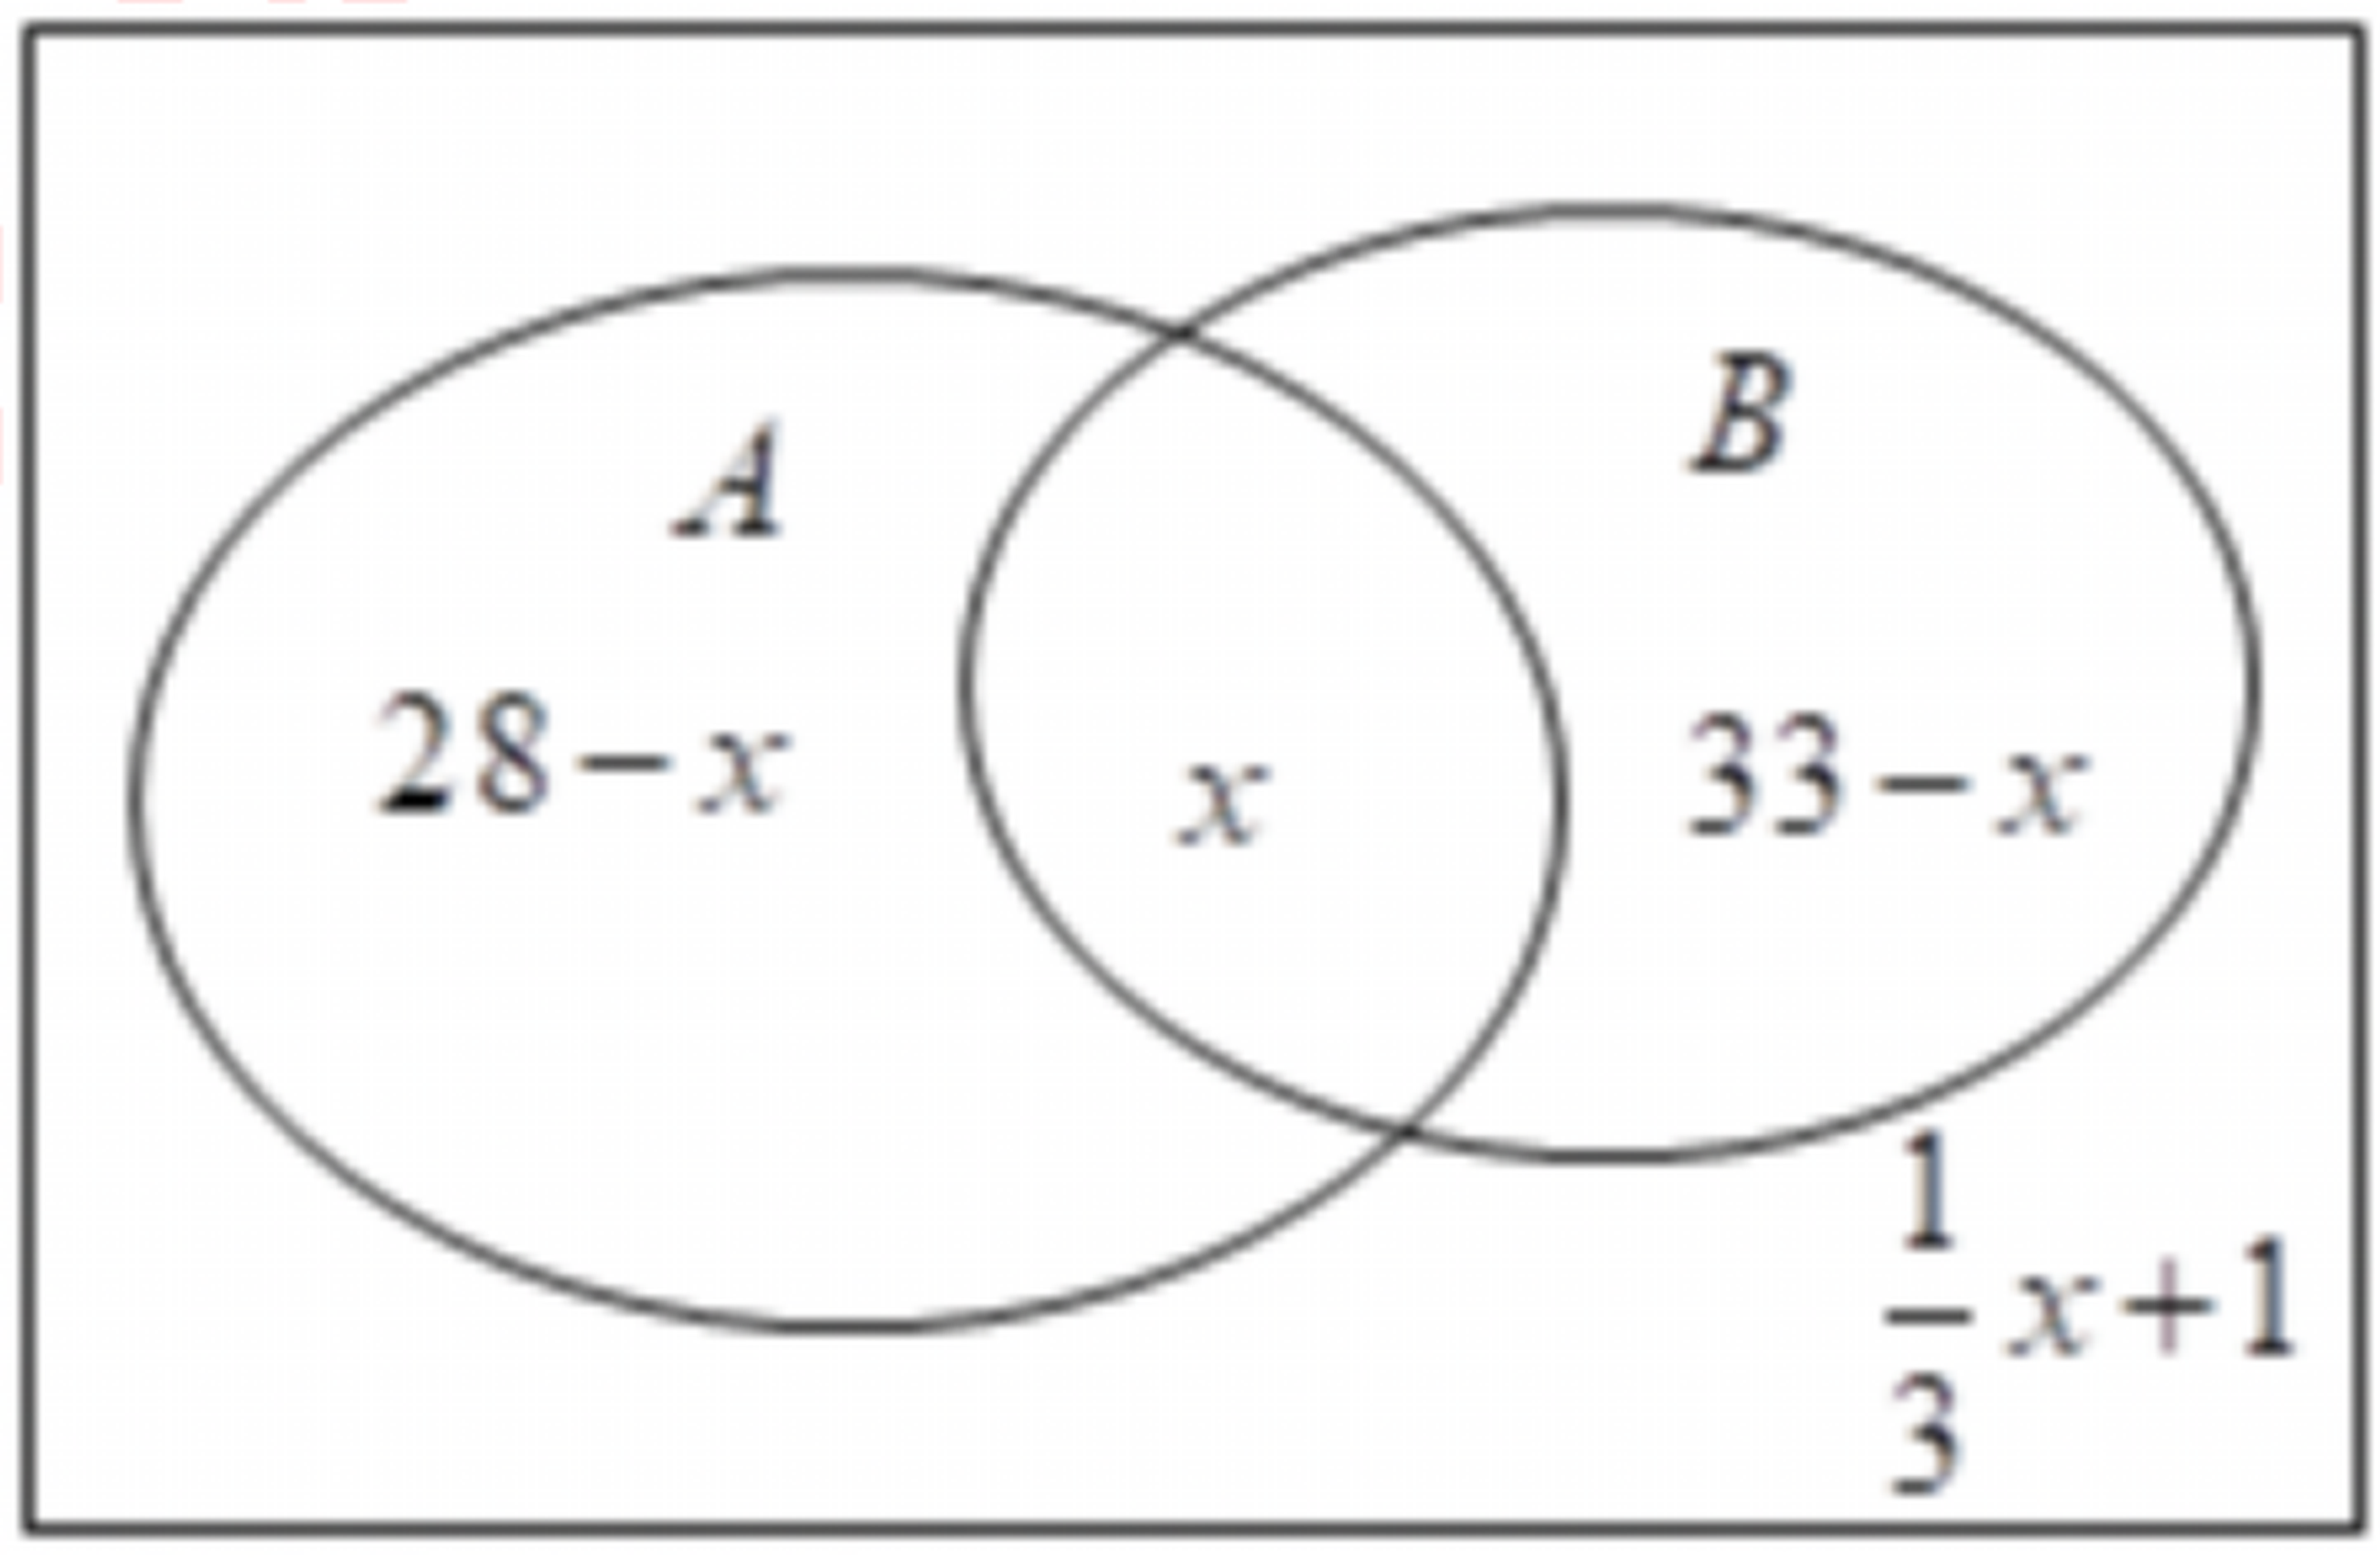
\includegraphics[width=0.42\textwidth]{figures/venn_AB_survey_50_x.png}
\end{center}
\step{则仅参加 $A$ 项的有 $(28-x)$ 人，仅参加 $B$ 项的有 $(33-x)$ 人，}
\step{$A$、$B$ 两项公益活动都不参加的有 $\left(\dfrac13x+1\right)$ 人，}
\step{由题意得 $x+(28-x)+(33-x)+\left(\dfrac13x+1\right)=50$，解得 $x=18$，}
\step{所以只参加 $A$ 项不参加 $B$ 项的有 $28-18=10$ 人.}
\solend
\fi

\item 设集合 $A=\{x\mid x^2-3x+2=0\}$，则满足 $A\cup B=\{0,1,2\}$ 的集合 $B$ 的个数是 \blankline[4.4em].

\ans{$4$}

\ifanswer
\solbegin
\step{$A=\{x\mid x^2-3x+2=0\}=\{x\mid x=1\text{ 或 }x=2\}=\{1,2\}$，}
\step{若 $A\cup B=\{0,1,2\}$，则 $0\in B$，}
\step{则 $B=\{0\},\{0,2\},\{1,0\},\{0,1,2\}$，共 $4$ 个.}
\solend
\fi

\item 已知全集 $U=\R$，集合 $A=\{x\mid x^2<4\}$，$B=\{y\mid y=x^2\}$，则图中阴影部分所表示的集合为 \blankline[4.4em].

\begin{center}
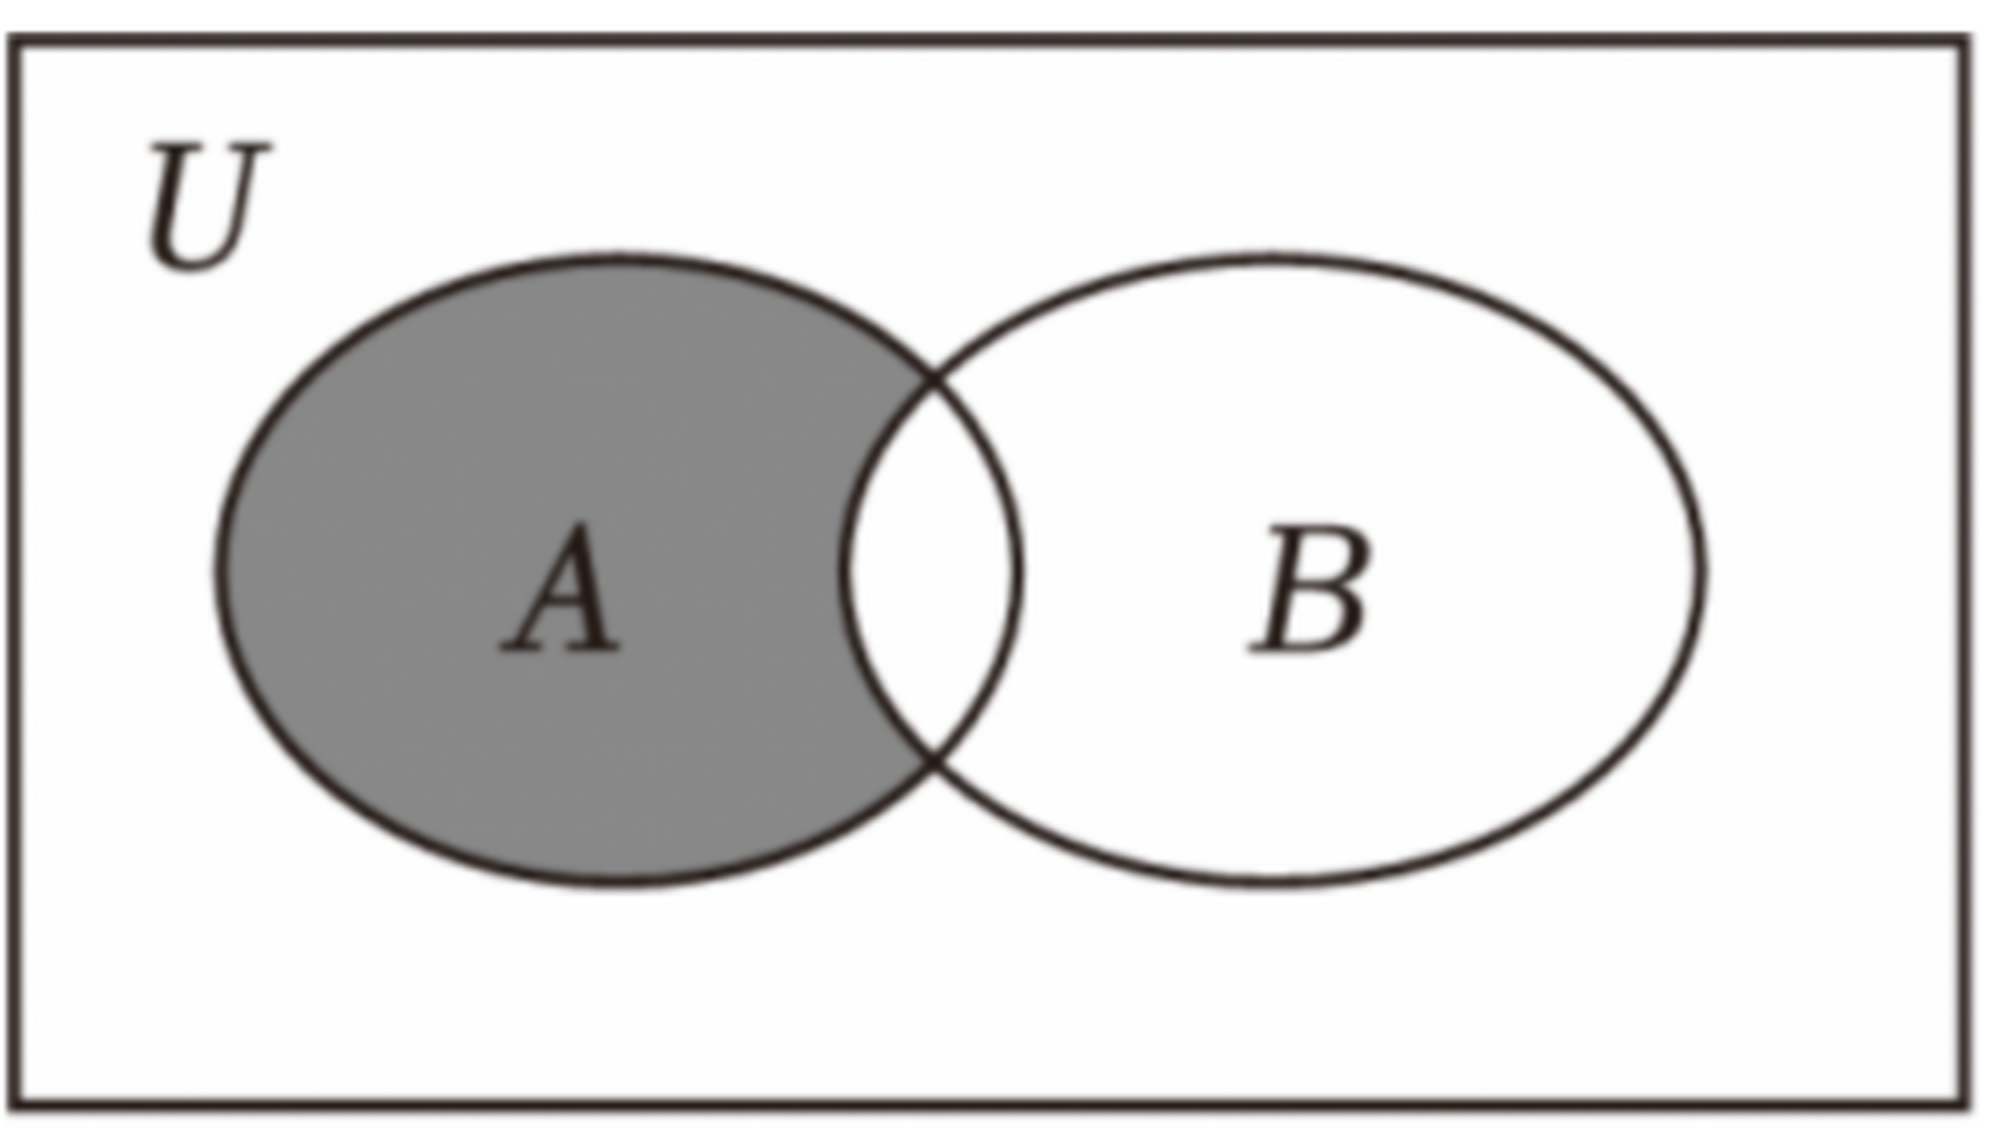
\includegraphics[width=0.34\textwidth]{figures/venn_A_shaded_U.png}
\end{center}

\ans{$A\cap\overline B=(-2,0)$}

\ifanswer
\solbegin
\step{集合 $A=\{x\mid x^2<4\}=(-2,2)$，$B=\{y\mid y=x^2\}=[0,+\infty)$，}
\step{图中阴影部分所表示的集合是 $A\cap\overline B=(-2,0)$.}
\solend
\fi

\item 如图所示，$M$、$P$、$S$ 是 $V$ 的三个子集，则阴影部分所表示的集合是 \blankline[5.4em].

\begin{center}
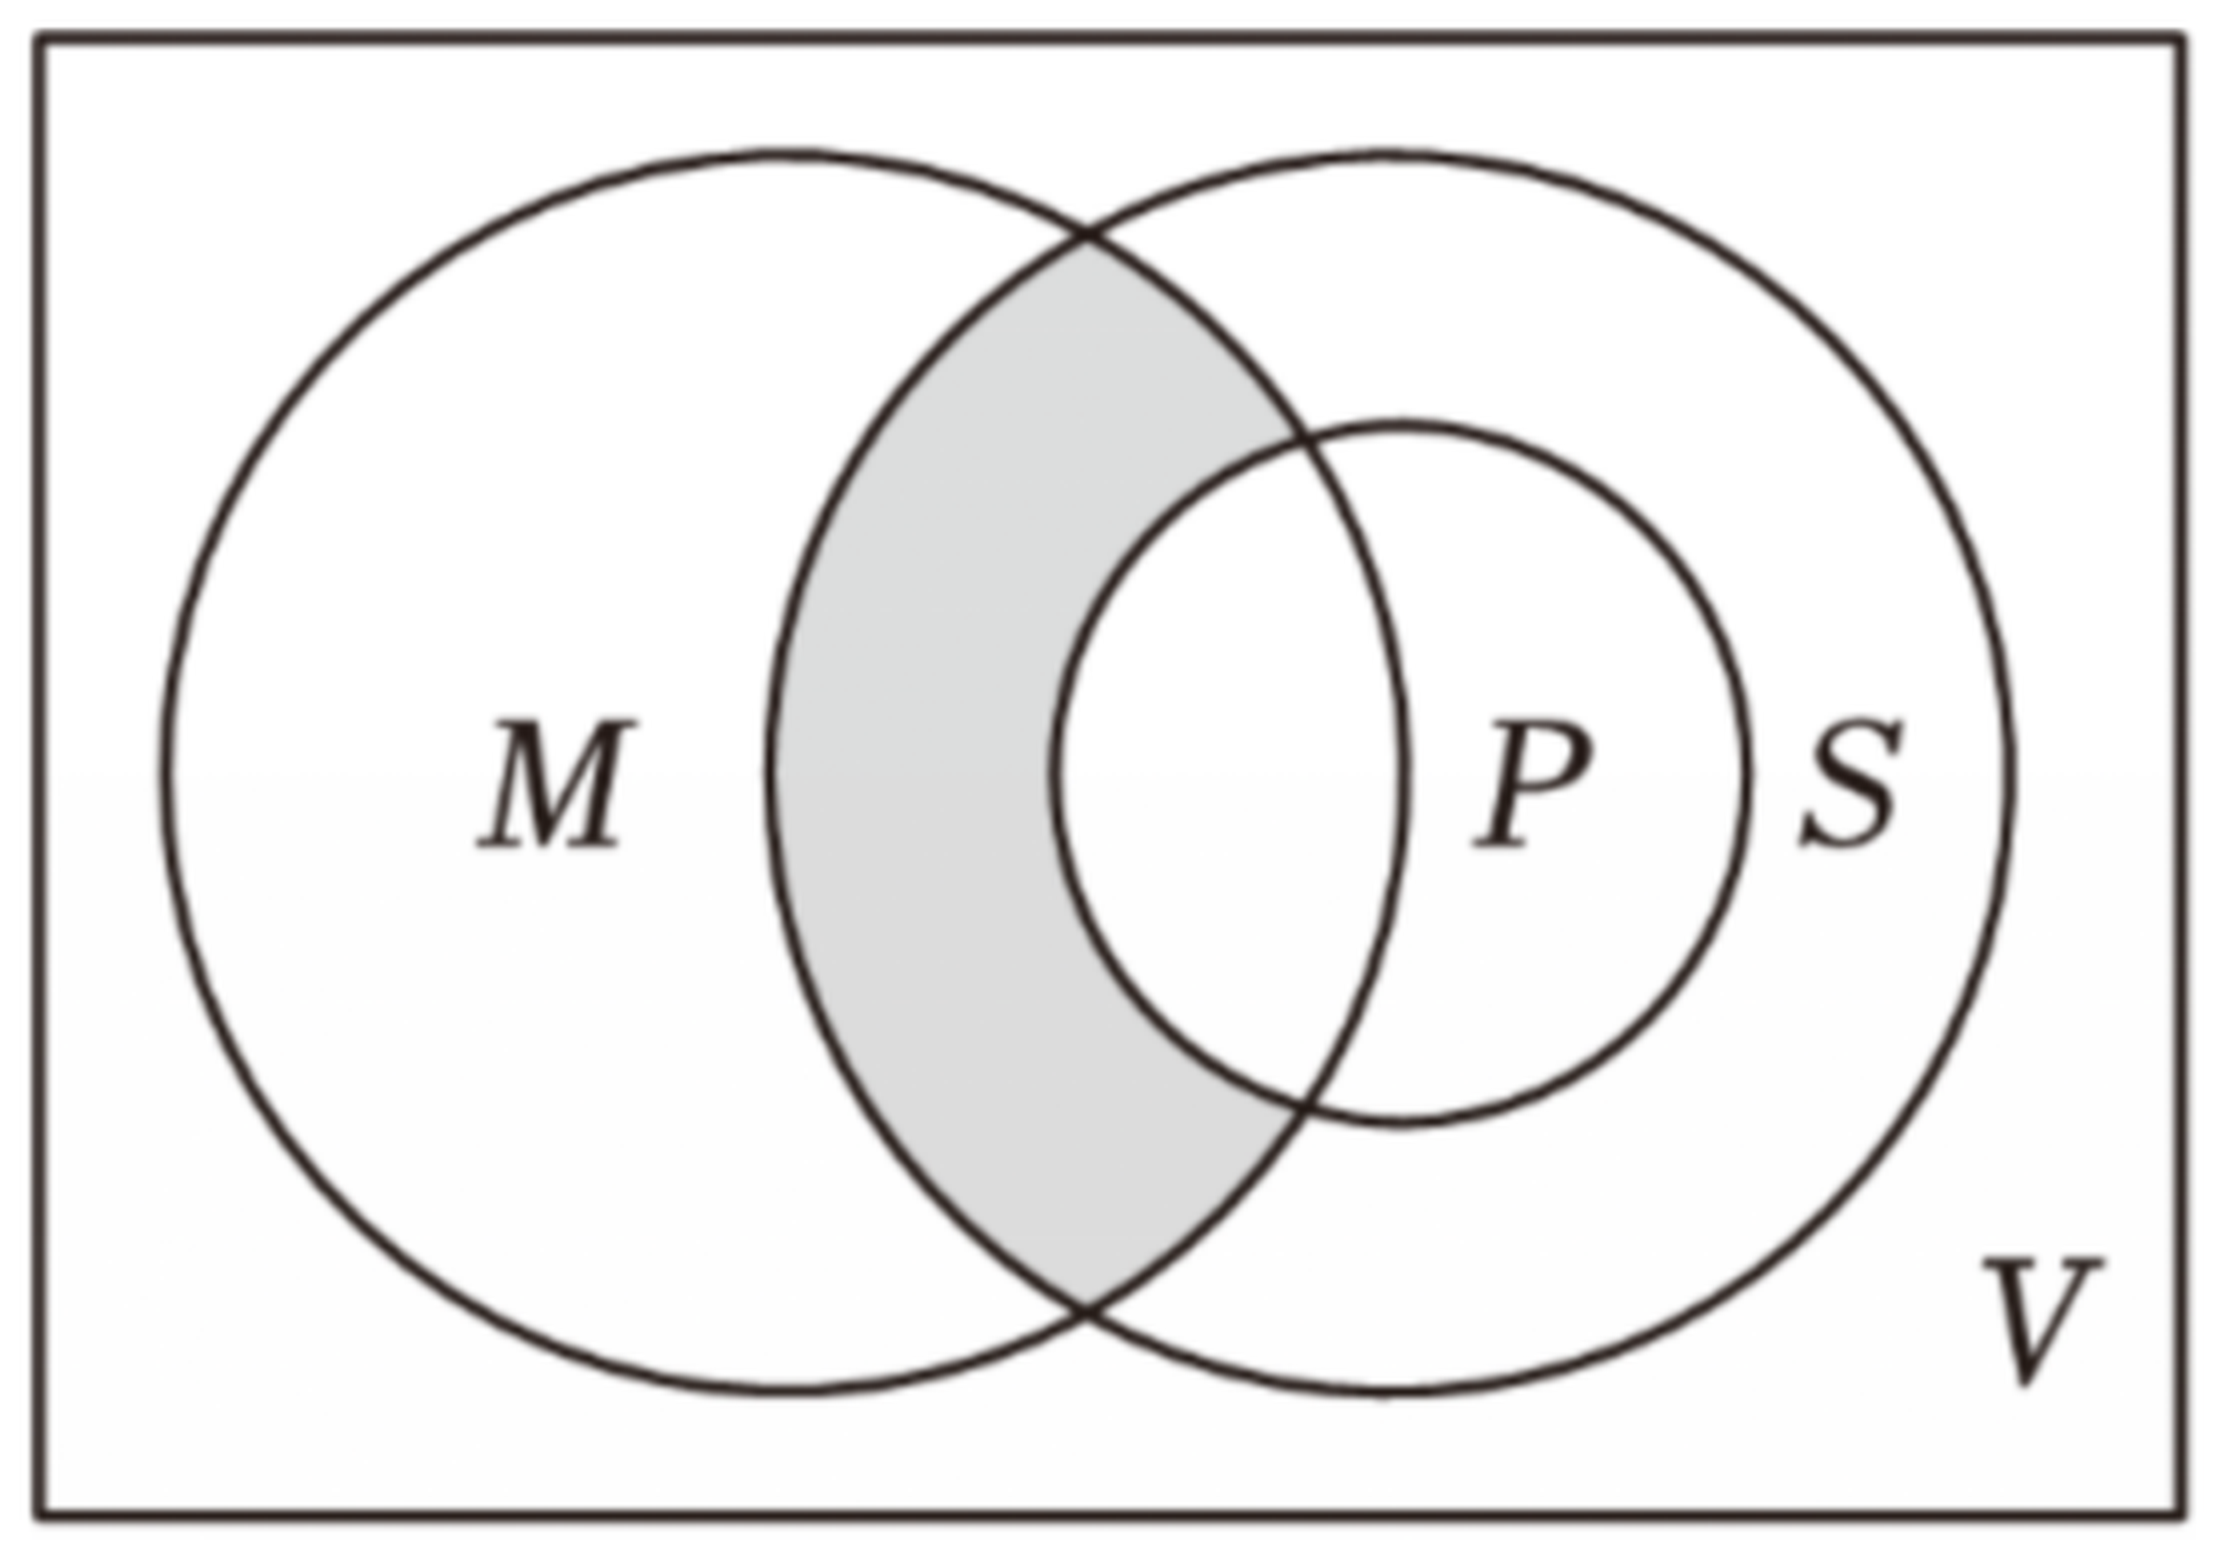
\includegraphics[width=0.38\textwidth]{figures/venn_MPS_V.png}
\end{center}

\ans{$(M\cap S)\cap(\complement_V P)$}

\item 下面六个关系式：① $\varnothing\subseteq\{a\}$；② $a\subseteq\{a\}$；③ $\{a\}\subseteq\{a\}$；④ $\{a\}\in\{a,b\}$；⑤ $a\in\{a,b,c\}$；⑥ $\varnothing\in\{a,b\}$；其中正确的是 \blankline[3.4em].

\ans{①③⑤}

\item 已知集合 $A=\{x\mid -1\le x\le a\}\ne\varnothing$，若 $\{y\mid y=x+1,x\in A\}=\{y\mid y=x^2,x\in A\}$，则实数 $a$ 值为 \blankline[4.4em].

\ans{$0$ 或 $\dfrac{1+\sqrt5}{2}$}

\ifanswer
\solbegin
\step{因为 $A=\{x\mid -1\le x\le a\}\ne\varnothing$，}
\step{所以 $\{y\mid y=x+1,x\in A\}=\{y\mid 0\le y\le a+1\}$，}
\step{$-1\le a\le1$ 时，$\{y\mid y=x^2,x\in A\}=\{y\mid 0\le y\le1\}$，}
\step{$a>1$ 时，$\{y\mid y=x^2,x\in A\}=\{y\mid 0\le y\le a^2\}$，}
\step{① $-1\le a\le1$ 时，$\{y\mid 0\le y\le a+1\}=\{y\mid 0\le y\le1\}$，则 $a+1=1$，解得 $a=0$；}
\step{② $a>1$ 时，$\{y\mid 0\le y\le a+1\}=\{y\mid 0\le y\le a^2\}$，则 $a^2=a+1$，解得 $a=\dfrac{1+\sqrt5}{2}$；}
\step{所以 $a=0$ 或 $\dfrac{1+\sqrt5}{2}$.}
\solend
\fi

\item 设集合 $A=\{(x,y)\mid x+y=22,x>0,y>0,x,y\text{ 均为质数}\}$ 的子集的个数为 \blankline[4.4em].

\ans{$32$}

\ifanswer
\solbegin
\step{集合 $A=\{(x,y)\mid x+y=22,x>0,y>0,x,y\text{ 均为质数}\}$}
\step{$=\{(3,19),(19,3),(5,17),(17,5),(11,11)\}$，则 $A$ 的子集的个数为 $2^5=32$.}
\solend
\fi

% 注：原卷本题题干印作「已知一个有四个数字元素的集合 $S$」；「数字元素」疑为「元素」之衍，
%     但原卷字形确为「数字」二字（已 3× 放大核对过），本稿照录，不代为改写。
\item 已知一个有四个数字元素的集合 $S$，$S$ 的所有子集的元素和（空集的元素和认为是 $0$）的总和为 $16192$，则 $S$ 的元素之和等于 \blankline[4.4em].

\ans{$2024$}

\ifanswer
\solbegin
\step{设 $S=\{a_1,a_2,a_3,a_4\}$，$S$ 的每个元素在所有子集中均出现 $2^3$ 次，}
\step{故 $(a_1+a_2+a_3+a_4)\cdot 2^3=16192$，所以 $a_1+a_2+a_3+a_4=2024$，}
\step{故 $S$ 的元素之和等于 $2024$.}
\solend
\fi

\item 设 $A$ 是非空数集，若对任意 $x$、$y\in A$，都有 $x+y\in A$、$xy\in A$，则称 $A$ 具有性质 $P$，给出以下命题：

①若 $A$ 具有性质 $P$，则 $A$ 可以是有限集；

②若 $A$ 具有性质 $P$，且 $A\ne\R$，则 $\overline A$ 具有性质 $P$；

③若 $A_1$、$A_2$ 具有性质 $P$，且 $A_1\cap A_2\ne\varnothing$，则 $A_1\cap A_2$ 具有性质 $P$；

④若 $A_1$、$A_2$ 具有性质 $P$，则 $A_1\cap A_2$ 具有性质 $P$.

其中所有真命题的序号是 \blankline[4.4em].

\ans{①③}

\ifanswer
\solbegin
\step{对于①，取集合 $A=\{0,1\}$ 具有性质 $P$，故 $A$ 可以是有限集，故①正确；}
\step{对于③，取 $x$、$y\in A_1\cap A_2$，则 $x\in A_1$，$x\in A_2$，$y\in A_1$，$y\in A_2$，}
\step{又 $A_1$、$A_2$ 具有性质 $P$，所以 $x+y\in A_1$，$xy\in A_1$，$x+y\in A_2$，$xy\in A_2$，}
\step{所以 $x+y\in A_1\cap A_2$，$xy\in A_1\cap A_2$，所以 $A_1\cap A_2$ 具有性质 $P$，故③正确；}
\step{对于④，取 $A_1=\{x\mid x=2k,k\in\Z\}$，$A_2=\{x\mid x=3k,k\in\Z\}$，$2\in A_1$，$3\in A_2$，}
\step{但 $2+3\notin A_1\cup A_2$，故④错误；}
\step{对于②，若 $A$ 具有性质 $P$，且 $A\ne\R$，假设 $\overline A$ 也具有性质 $P$，}
\step{设 $0\in A$，在 $\overline A$ 中任取一个 $x$，$x\ne0$，此时可证得 $-x\in A$，}
\step{否则若 $-x\in\overline A$，由于 $\overline A$ 也具有性质 $P$，则 $x+(-x)=0\in\overline A$，}
\step{与 $0\in A$ 矛盾，故 $-x\in A$，}
\step{由于 $A$ 具有性质 $P$，$\overline A$ 也具有性质 $P$，所以 $(-x)^2\in A$，$x^2\in\overline A$，}
\step{而 $(-x)^2=x^2$，这与 $A\cap\overline A=\varnothing$ 矛盾，}
\step{故当 $0\in A$ 且 $A$ 具有性质 $P$ 时，则 $\overline A$ 不具有性质 $P$，}
\step{同理当 $0\in\overline A$ 时，也可以类似推出矛盾，故②错误.}
\step{故正确的是①③.}
\solend
\fi

\item 已知 $S=\{1,2,3,4,5\}$，$A=\{1,2,5\}$，$T=\{t_1,t_2\}\subseteq S$，记 $A_1=\{x\mid x=a+t_1,a\in A,t_1\in T\}$，$A_2=\{x\mid x=b+t_2,b\in A,t_2\in T\}$，若 $A_1\cap A_2=\varnothing$，则集合 $T$ 为 \blankline[5.4em].

\ans{$T=\{1,3\}$ 或 $T=\{2,4\}$ 或 $T=\{3,5\}$}

\ifanswer
\solbegin
\step{若 $A_1\cap A_2=\varnothing$，即 $a+t_1\ne b+t_2$，则 $t_1-t_2\ne a-b$，其中 $a$、$b\in A$，}
\step{否则 $t_1+a=t_2+b$，$A_1\cap A_2\ne\varnothing$，}
\step{又 $S=\{1,2,3,4,5\}$，$A=\{1,2,5\}$，$T=\{t_1,t_2\}\subseteq S$，}
\step{$2-1=1$，$5-2=3$，$5-1=4$，则 $t_1$、$t_2$ 相差 $2$，}
\step{所以 $T=\{1,3\}$ 或 $T=\{2,4\}$ 或 $T=\{3,5\}$.}
\solend
\fi

\end{enumerate}

\bigsec{二、解答题}

\begin{enumerate}
\setcounter{enumi}{13}

\item 设集合 $P=\{1,2,3,m\}$，$Q=\{3,m^2\}$，且 $\overline P\cap Q=\varnothing$，求实数 $m$ 的值组成的集合.

\ans{$\{-1,0,\pm\sqrt2\}$}

\ansspace[5]

\ifanswer
\solbegin
\step{因为 $\overline P\cap Q=\varnothing$，所以 $Q\subseteq P$，所以 $m^2=1$ 或 $m^2=2$ 或 $m^2=m$，}
\step{考虑互异性，得 $m=-1$ 或 $m=\pm\sqrt2$ 或 $m=0$，}
\step{所以实数 $m$ 的值组成的集合为 $\{-1,0,\pm\sqrt2\}$.}
\solend
\fi

\item 若集合 $A=(-\infty,2]$，$B=\{x\mid kx+1<0,k\in\R\}$，$A\cap B=\varnothing$，求实数 $k$ 的取值范围.

\ans{$\left[-\dfrac12,0\right]$}

\ansspace[5]

\ifanswer
\solbegin
\step{若 $B=\varnothing$，则 $k=0$，符合题意，}
\step{若 $B\ne\varnothing$，当 $k>0$ 时，$B=\left(-\infty,-\dfrac1k\right)$，$A\cap B\ne\varnothing$，不合题意；}
\step{当 $k<0$ 时，$B=\left(-\dfrac1k,+\infty\right)$，由 $A\cap B=\varnothing$ 得 $-\dfrac1k\ge2$，即 $-\dfrac12\le k<0$，}
\step{故 $k$ 的取值范围是 $\left[-\dfrac12,0\right]$.}
\solend
\fi

\item 已知集合 $A=\{-4,2a-1,a^2\}$，$B=\{a-5,1-a,9\}$，分别求适合下列条件的 $a$ 的值.

% 两个小问不许与题干分家：试卷版第 2 页页末原本正好把 (1) 留在页底、(2) 翻到次页，
% 与 2026-09-15 修的三类难看切页同源，故在这里也加 \keepwithprev 守卫（三版都生效）。
\keepwithprev
（1）$9\in(A\cap B)$；

\keepwithprev
（2）$\{9\}=A\cap B$.

\ans{（1）$a=5$ 或 $a=-3$；（2）$a=-3$}

\ansspace[5]

\ifanswer
\solbegin
\stepm{（1）}{$9\in(A\cap B)$，所以 $9\in A$，}
\step{当 $2a-1=9$ 时，$a=5$，当 $a^2=9$ 时，即 $a=\pm3$，}
% 注：原卷此句结论印作「所以 $a$ 的值为 $5\backslash-3$」——「\」应是顿号之误，
%     本稿照录原卷字形（见文件头「原卷存疑」②）；按文意即 $a=5$ 或 $a=-3$。
\step{当 $a=3$ 时，$a-5=1-a$ 舍去，所以 $a$ 的值为 $5\backslash-3$.}
\stepm{（2）}{结合（1）的结论：}
\step{当 $2a-1=9$ 即 $a=5$ 时，$1-a=-4$，$\{9\}\ne(A\cap B)$，}
\step{当 $a^2=9$ 时，即 $a=\pm3$，当 $a=3$ 时，$a-5=1-a$ 舍去，}
\step{所以 $a$ 的值为 $-3$.}
\solend
\fi

\item 已知集合 $M=\{a,ab,a-b\}$，$N=\{0,|a|,b\}$，且 $M=N$，求实数 $a$、$b$ 的值.

\ans{$a=b=-1$}

\ansspace[5]

\ifanswer
\solbegin
\step{由集合元素的互异性，得 $a\ne0$，且 $b\ne0$，所以 $a-b=0$，即 $a=b$，}
\step{所以 $ab=|a|$，又由 $|a|\ne b=a$，得 $a<0$，故 $a=b=-1$.}
\solend
\fi

\item 已知集合 $A=\{x\mid -2<x<7\}$，$B=\{x\mid m+1\le x\le 2m-1\}$.

\keepwithprev
（1）当 $m=4$ 时，求 $A\cap B$、$A\cup B$；

\keepwithprev
（2）若 $A\cap B=B$，求实数 $m$ 的取值范围.

\ans{（1）$A\cap B=[5,7)$，$A\cup B=(-2,7]$；（2）$(-\infty,4)$}

\ansspace[5]

\ifanswer
\solbegin
\stepm{（1）}{当 $m=4$ 时，得集合 $A=\{x\mid -2<x<7\}$，$B=\{x\mid 5\le x\le7\}$，}
\step{得 $A\cap B=[5,7)$，$A\cup B=(-2,7]$.}
\stepm{（2）}{由 $A\cap B=B$ 得 $B\subseteq A$，}
\step{①当 $B=\varnothing$ 时，得 $m+1>2m-1$，解得 $m<2$；}
\step{②当 $B\ne\varnothing$ 时，得 $\begin{cases}m+1>-2\\ 2m-1<7\\ m+1\le2m-1\end{cases}$，解得 $2\le m<4$；}
\step{综上，实数 $m$ 的取值范围是 $(-\infty,4)$.}
\solend
\fi

\item 若集合 $A=\{x\mid x^2+5x-6=0\}$，$B=\{x\mid x^2+2(m+1)x+m^2-3=0\}$.

\keepwithprev
（1）当 $m=0$ 时，求集合 $A\cup B$；

\keepwithprev
（2）若 $A\cap B=B$，求实数 $m$ 的取值范围.

\ans{（1）$A\cup B=\{1,-6,-3\}$；（2）$\{m\mid m\le-2\}$}

\ansspace[5]

\ifanswer
\solbegin
\stepm{（1）}{由题意得，集合 $A=\{x\mid x^2+5x-6=0\}=\{1,-6\}$，}
\step{当 $m=0$ 时，$B=\{x\mid x^2+2x-3=0\}=\{1,-3\}$，}
\step{所以 $A\cup B=\{1,-6,-3\}$；}
\stepm{（2）}{由（1）得集合 $A=\{1,-6\}$，$B=\{x\mid x^2+2(m+1)x+m^2-3=0\}$，}
\step{若 $A\cap B=B$ 得 $B\subseteq A$，所以 $B=\varnothing$ 或 $\{-6\}$ 或 $\{1\}$ 或 $\{1,-6\}$，}
\step{当 $B=\varnothing$ 时，$\Delta=4(m+1)^2-4(m^2-3)<0$，解得 $m<-2$，}
\step{当 $B=\{-6\}$ 时，则 $\begin{cases}\Delta=4(m+1)^2-4(m^2-3)=0\\ 36-12(m+1)+m^2-3=0\end{cases}$，无解，}
\step{当 $B=\{1\}$ 时，则 $\begin{cases}\Delta=4(m+1)^2-4(m^2-3)=0\\ 1+2(m+1)+m^2-3=0\end{cases}$，解得 $m=-2$，}
\step{当 $B=\{1,-6\}$ 时，则 $\begin{cases}\Delta=4(m+1)^2-4(m^2-3)>0\\ 1+(-6)=-2(m+1)\\ 1\times(-6)=m^2-3\end{cases}$，无解，}
\step{综上所述，实数 $m$ 的取值范围为 $\{m\mid m\le-2\}$.}
\solend
\fi

% 压轴题：其后已无内容，故作答区全用可丢弃胶水（\ansspace*），并在题目前先量一下版面。
\ansneed{8cm}
\item 对于点集 $A=\{(x,y)\mid x=m,y=-3x+2,m\in\N,m\ge1\}$，$B=\{(x,y)\mid x=n,y=a(x^2-x+1),n\in\N,n\ge1\}$，是否存在非零整数 $a$，使得 $A\cap B\ne\varnothing$？

\ans{$a=-1$}

\ansspace*[10]

\ifanswer
\solbegin
\step{当 $A\cap B\ne\varnothing$ 时，$-3x+2=a(x^2-x+1)$，}
\step{$ax^2+(3-a)x+a-2=0$ ①有正整数解，}
\step{所以 $\Delta=(3-a)^2-4a(a-2)=-3a^2+2a+9$ 是平方数，}
\step{所以 $3a^2-2a-9\le0$，$\dfrac{1-2\sqrt7}{3}\le a\le\dfrac{1+2\sqrt7}{3}$，$a\ne0$，$a\in\Z$，}
\step{所以 $a=\pm1$ 或 $a=2$，}
\step{$a=-1$ 时 $\Delta=4$，这时①变为 $-x^2+4x-3=0$，解得 $x_1=1$，$x_2=3$，}
\step{$A\cap B=\{(1,-1),(3,-7)\}$.}
\step{$a=1$ 时 $\Delta=8$，不是平方数.}
\step{$a=2$ 时 $\Delta=1$，这时①变为 $2x^2+x=0$，没有正整数解.}
\step{所以 $a=-1$.}
\solend
\fi

\end{enumerate}

\end{document}
"
%
% 原始材料是微信公众号图文（公众号「魔都数学加油站」，作者署名「破晓」，
% 原文链接 https://mp.weixin.qq.com/s/tHqWSV1StO5SHSXXQ4jeUA），正文为 6 张 PNG 页；
% 原文本身就是一份**讲评版**——题目下方直接印出【答案】或【解析】。本稿把答案与解析
% 移到答案版，试卷版即一张干净的空卷；试题文字、答案与解析均照原卷录入。
%
% 与原卷的排版差异（均已在 README「说明」中交代）：
%   ① 原文自**第 3 题**起（第 1、2 题未在该文发布），源码里以 \setcounter{enumi}{2} 起编；
%      全卷只有「一、填空题」「二、解答题」两节，无选择题；
%   ② 原卷本就印有两个分节标题（已在原图上逐页放大核对过），本稿照原卷分节，只把标题改排
%      成全稿统一的「大节标题」样式；
%   ③ 原卷的实数集、整数集、自然数集符号作正体 $R$、$Z$、$N$（第 15 题作粗体 $\mathbf{R}$，
%      第 20 题有 $N$ 与斜体 $Z$），本稿按全稿惯例统一写作 $\R$、$\Z$、$\N$；
%   ④ 第 4 题的韦恩图在原卷里印在【解析】右侧（题干并无「如图」二字），故本稿把该图放进
%      答案版的解析块内（`figures/venn_AB_survey_50_x.png`）；第 6、7 题的韦恩图是**题干图**
%      （题干作「图中阴影部分所表示的集合」），两版都排（`figures/venn_A_shaded_U.png`、
%      `figures/venn_MPS_V.png`）。三张图都取自原卷截图、4× LANCZOS 放大，不用 TikZ 手绘；
%   ⑤ 本卷也是「讲评版」，解析按全稿统一的 \solbegin/\step 分步重排（原卷为连续段落），
%      分步不改一字，只断句、断行；
%   ⑥ 标题前缀照**原卷**作「2026--2027 年…」（原卷标题即作「2026-2027年延安中学高一上周末
%      作业 2」）。同校的 高一06 作「学年度」——那是 高一02—高一09 那一批入库时统一改的；
%      后续入库的卷（高一10—高一17 与本卷）一律照原卷保留「年」，未强改，故同校两卷前缀不同。
%
% 原卷存疑两处（已逐处放大到能看清字形后核对，本稿照录并加注，见各题下的 `%` 注）：
%   （另有第三处「第 12 题【解析】末句」原先记作存疑，2026-09-26 第二轮核对放大后发现
%     原卷印的是「$0\in\overline A$」——A 上确有横杠，是本稿当初漏抄了 $\overline{}$；
%     已按原卷补回，故该条从存疑清单里删去，不计为原卷问题。）
%   ① 第 11 题题干印作「已知一个有四个数字元素的集合 $S$」，「数字元素」疑为「元素」之衍；
%   ② 第 16 题 (1) 结论印作「$a$ 的值为 $5\backslash-3$」，其中的「\」应是顿号之误
%      （由 (2) 的结论「$a$ 的值为 $-3$」可反推，(1) 的答案是 $5$ 或 $-3$）；

% 本篇在公众号「魔都数学加油站」连载里的编号是「27学年高一19」，本地编号与之对齐（高一19）；
% 对应关系见 README「与公众号连载号的对照表」。
\documentclass[a4paper,11pt]{article}
\usepackage{common}

\begin{document}

\examtitlest{2026--2027 年延安中学高一上周末作业 2}{集合与常用逻辑用语}

\bigsec{一、填空题}

\begin{enumerate}
% 原卷填空题从第 3 题起（1、2 未在该文中发布），须与解答题的 \setcounter{enumi}{13} 对齐
\setcounter{enumi}{2}
\item 已知全集 $U=\{1,2,3,4,5\}$，$M=\{1,2\}$，$P=\{1,3,5\}$，则 $M\cap\overline P=$ \blankline[4.4em].

\ans{$\{2\}$}

\item 某公司共有 $50$ 人，此次组织参加社会公益活动，其中参加 $A$ 项公益活动的有 $28$ 人，参加 $B$ 项公益活动的有 $33$ 人，且 $A$、$B$ 两项公益活动都不参加的人数比都参加的人数的三分之一多 $1$ 人，则只参加 $A$ 项不参加 $B$ 项的人数是 \blankline[4.4em].

\ans{$10$}

\ifanswer
\solbegin
\step{如图所示，设 $A$、$B$ 两项公益活动都参加的有 $x$ 人，}
\begin{center}
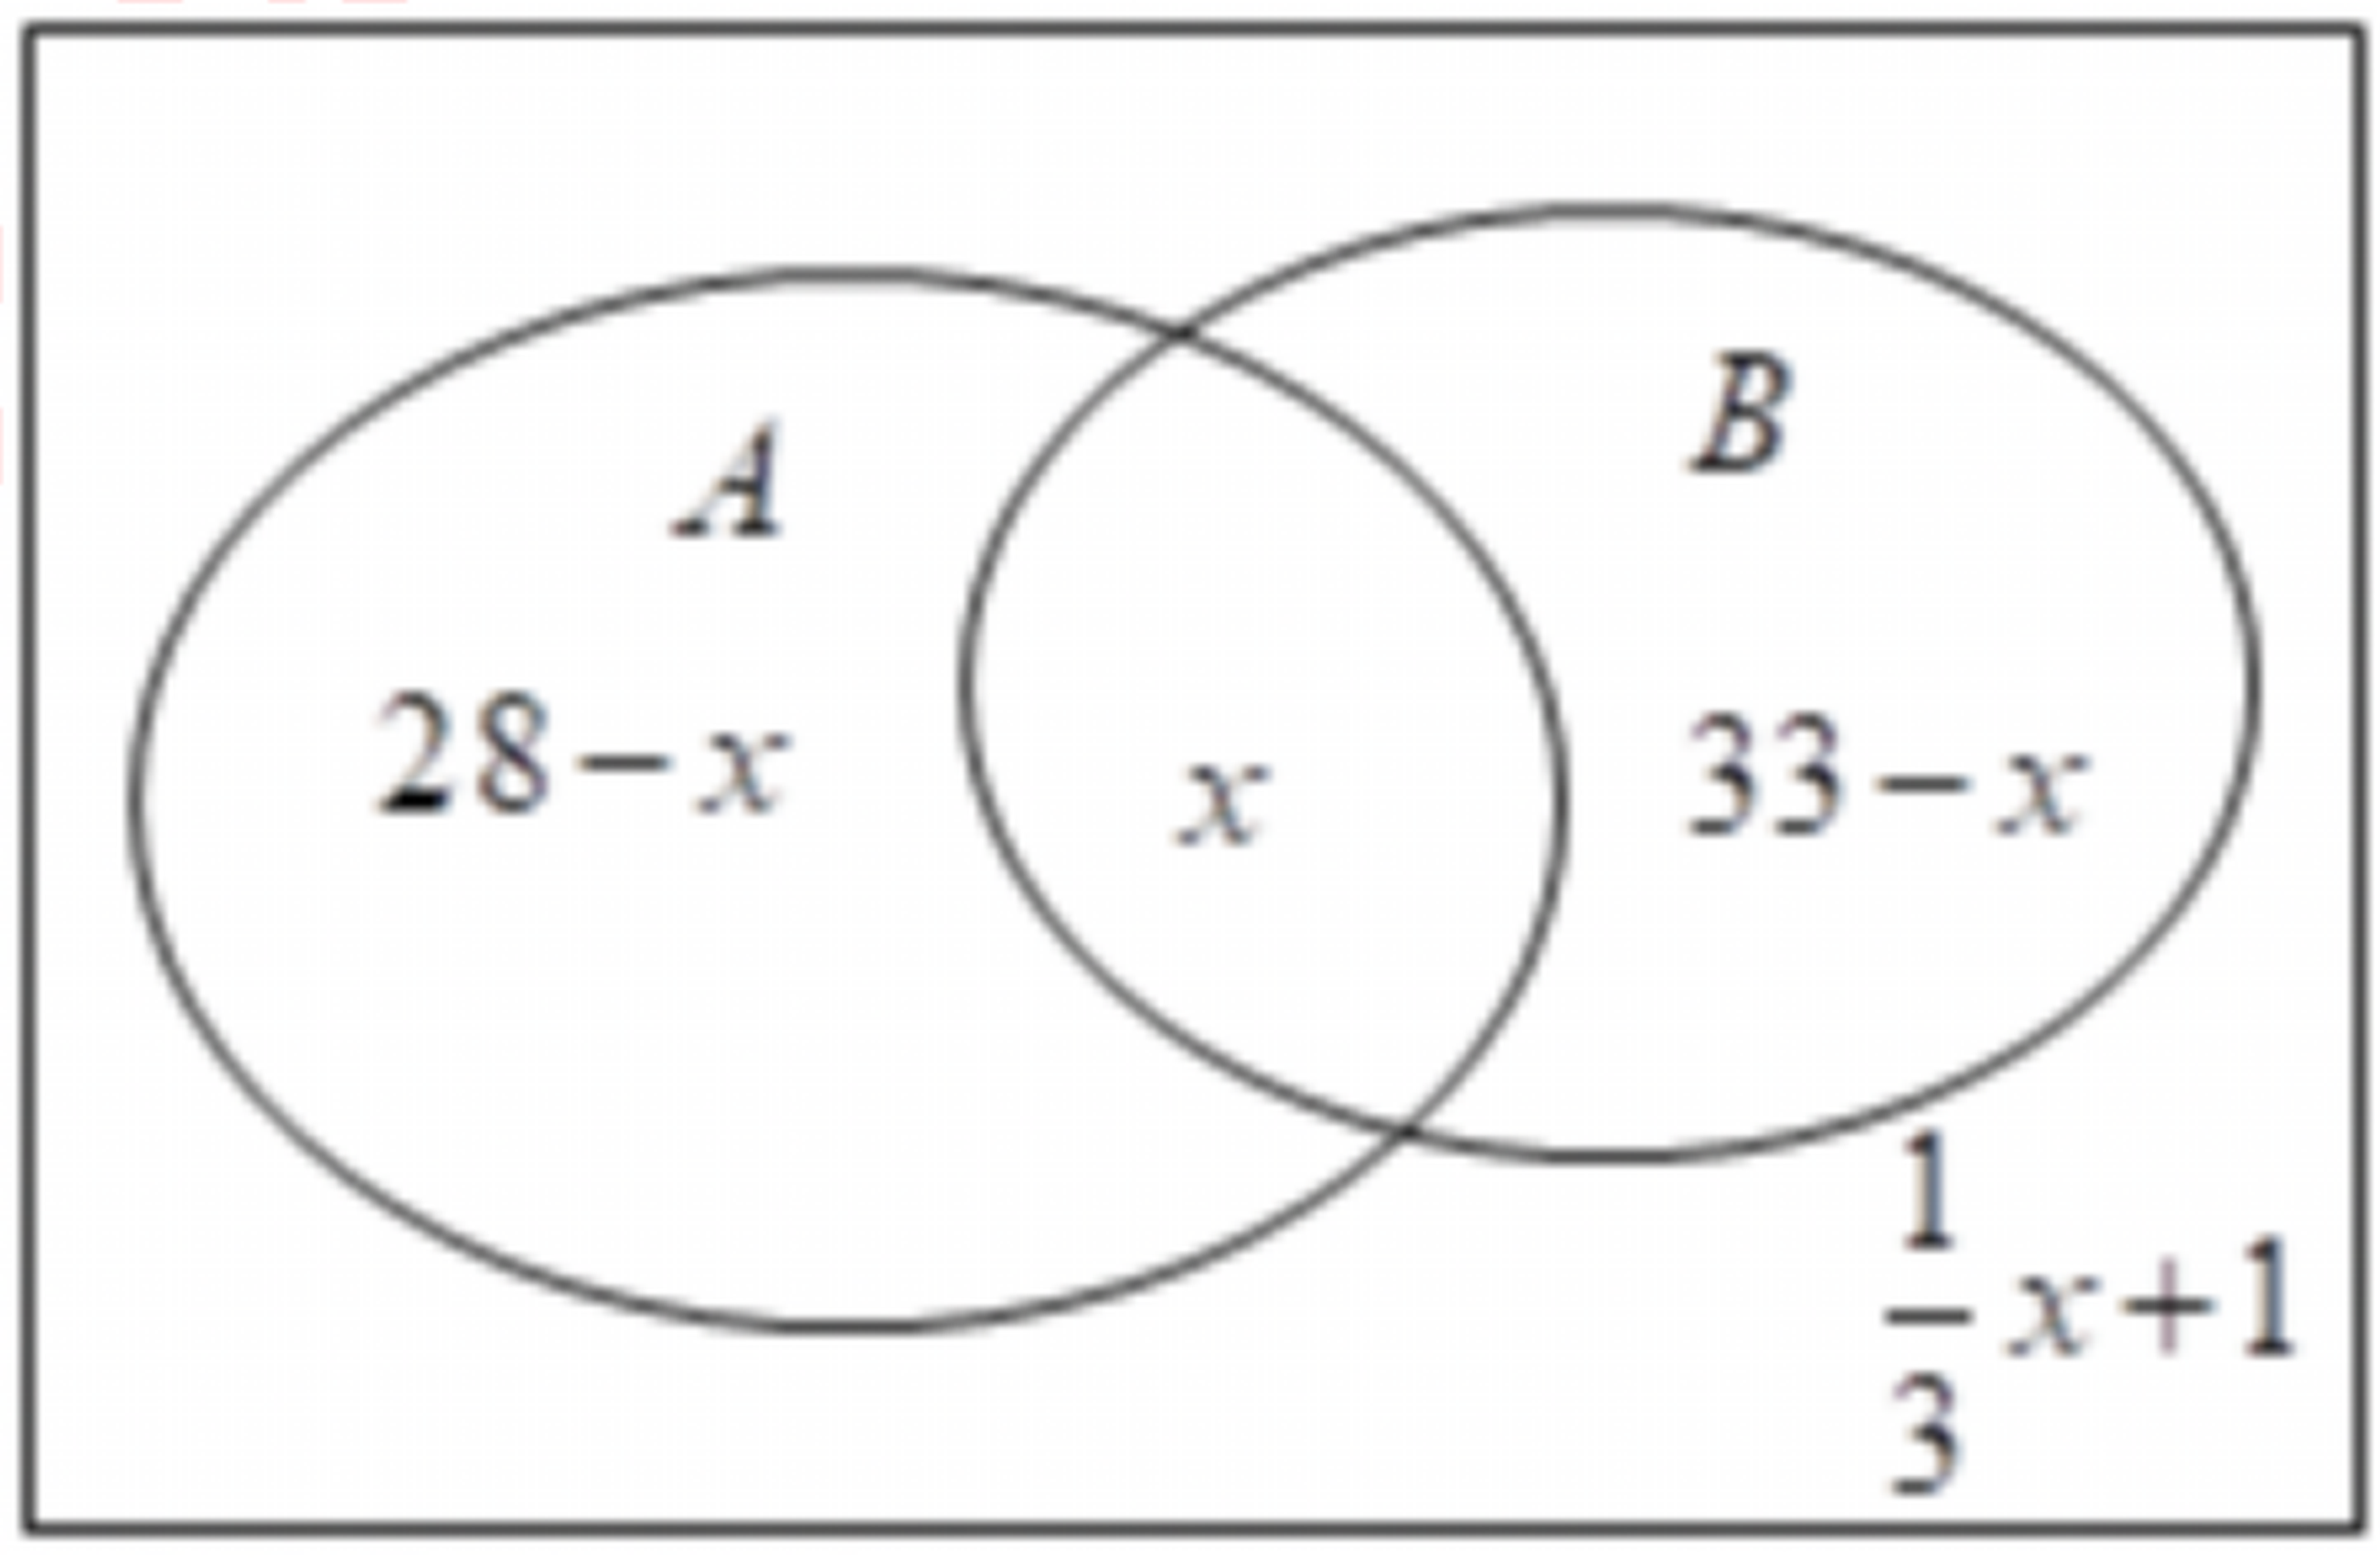
\includegraphics[width=0.42\textwidth]{figures/venn_AB_survey_50_x.png}
\end{center}
\step{则仅参加 $A$ 项的有 $(28-x)$ 人，仅参加 $B$ 项的有 $(33-x)$ 人，}
\step{$A$、$B$ 两项公益活动都不参加的有 $\left(\dfrac13x+1\right)$ 人，}
\step{由题意得 $x+(28-x)+(33-x)+\left(\dfrac13x+1\right)=50$，解得 $x=18$，}
\step{所以只参加 $A$ 项不参加 $B$ 项的有 $28-18=10$ 人.}
\solend
\fi

\item 设集合 $A=\{x\mid x^2-3x+2=0\}$，则满足 $A\cup B=\{0,1,2\}$ 的集合 $B$ 的个数是 \blankline[4.4em].

\ans{$4$}

\ifanswer
\solbegin
\step{$A=\{x\mid x^2-3x+2=0\}=\{x\mid x=1\text{ 或 }x=2\}=\{1,2\}$，}
\step{若 $A\cup B=\{0,1,2\}$，则 $0\in B$，}
\step{则 $B=\{0\},\{0,2\},\{1,0\},\{0,1,2\}$，共 $4$ 个.}
\solend
\fi

\item 已知全集 $U=\R$，集合 $A=\{x\mid x^2<4\}$，$B=\{y\mid y=x^2\}$，则图中阴影部分所表示的集合为 \blankline[4.4em].

\begin{center}
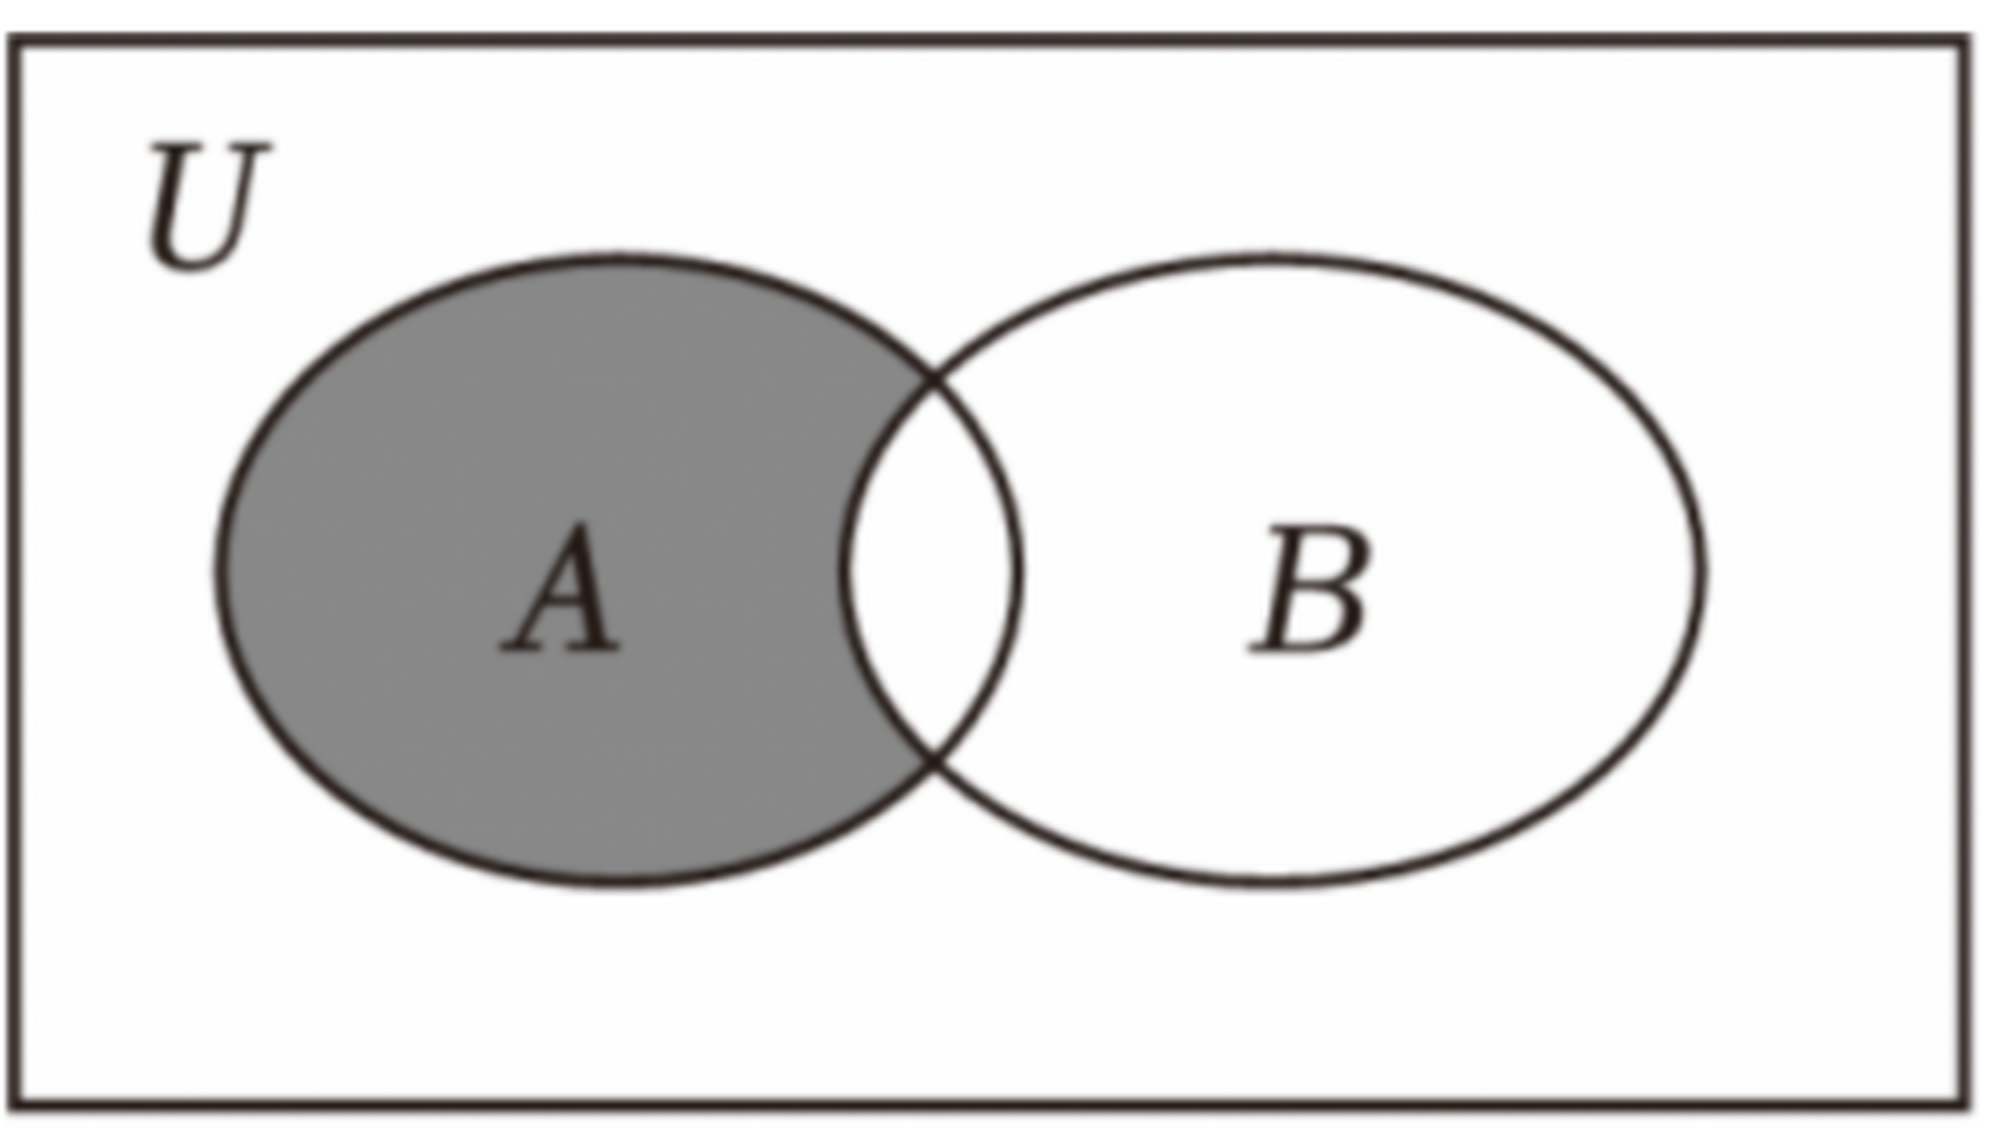
\includegraphics[width=0.34\textwidth]{figures/venn_A_shaded_U.png}
\end{center}

\ans{$A\cap\overline B=(-2,0)$}

\ifanswer
\solbegin
\step{集合 $A=\{x\mid x^2<4\}=(-2,2)$，$B=\{y\mid y=x^2\}=[0,+\infty)$，}
\step{图中阴影部分所表示的集合是 $A\cap\overline B=(-2,0)$.}
\solend
\fi

\item 如图所示，$M$、$P$、$S$ 是 $V$ 的三个子集，则阴影部分所表示的集合是 \blankline[5.4em].

\begin{center}
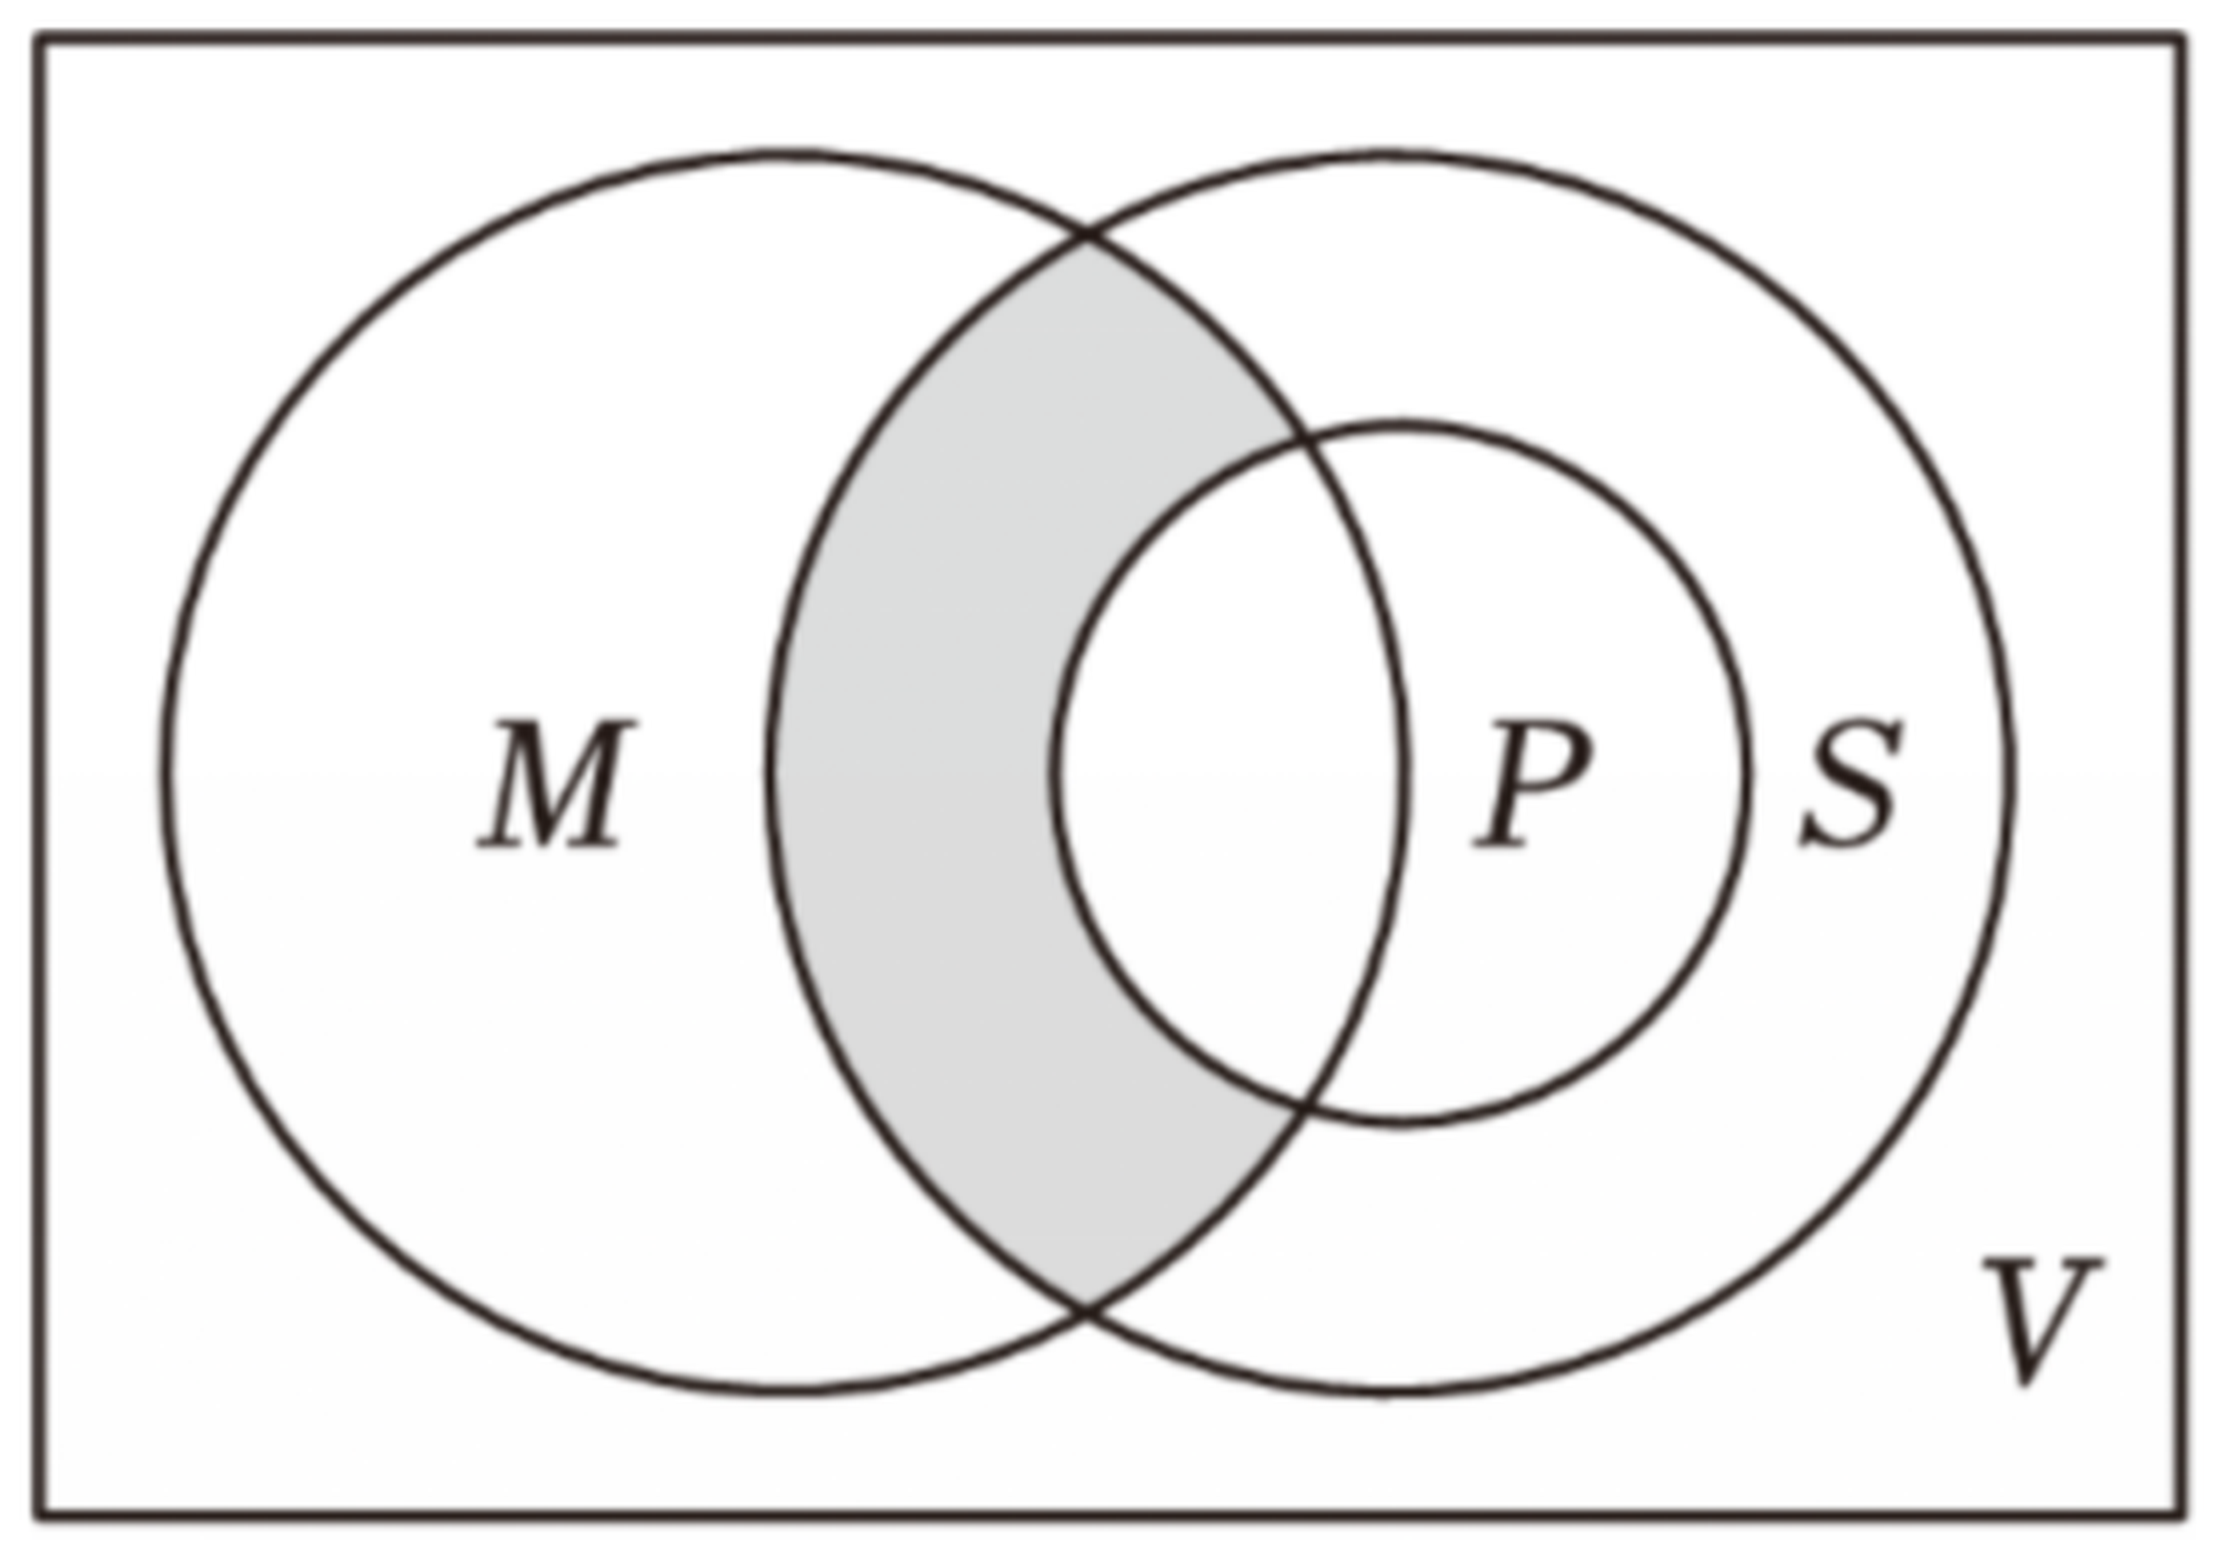
\includegraphics[width=0.38\textwidth]{figures/venn_MPS_V.png}
\end{center}

\ans{$(M\cap S)\cap(\complement_V P)$}

\item 下面六个关系式：① $\varnothing\subseteq\{a\}$；② $a\subseteq\{a\}$；③ $\{a\}\subseteq\{a\}$；④ $\{a\}\in\{a,b\}$；⑤ $a\in\{a,b,c\}$；⑥ $\varnothing\in\{a,b\}$；其中正确的是 \blankline[3.4em].

\ans{①③⑤}

\item 已知集合 $A=\{x\mid -1\le x\le a\}\ne\varnothing$，若 $\{y\mid y=x+1,x\in A\}=\{y\mid y=x^2,x\in A\}$，则实数 $a$ 值为 \blankline[4.4em].

\ans{$0$ 或 $\dfrac{1+\sqrt5}{2}$}

\ifanswer
\solbegin
\step{因为 $A=\{x\mid -1\le x\le a\}\ne\varnothing$，}
\step{所以 $\{y\mid y=x+1,x\in A\}=\{y\mid 0\le y\le a+1\}$，}
\step{$-1\le a\le1$ 时，$\{y\mid y=x^2,x\in A\}=\{y\mid 0\le y\le1\}$，}
\step{$a>1$ 时，$\{y\mid y=x^2,x\in A\}=\{y\mid 0\le y\le a^2\}$，}
\step{① $-1\le a\le1$ 时，$\{y\mid 0\le y\le a+1\}=\{y\mid 0\le y\le1\}$，则 $a+1=1$，解得 $a=0$；}
\step{② $a>1$ 时，$\{y\mid 0\le y\le a+1\}=\{y\mid 0\le y\le a^2\}$，则 $a^2=a+1$，解得 $a=\dfrac{1+\sqrt5}{2}$；}
\step{所以 $a=0$ 或 $\dfrac{1+\sqrt5}{2}$.}
\solend
\fi

\item 设集合 $A=\{(x,y)\mid x+y=22,x>0,y>0,x,y\text{ 均为质数}\}$ 的子集的个数为 \blankline[4.4em].

\ans{$32$}

\ifanswer
\solbegin
\step{集合 $A=\{(x,y)\mid x+y=22,x>0,y>0,x,y\text{ 均为质数}\}$}
\step{$=\{(3,19),(19,3),(5,17),(17,5),(11,11)\}$，则 $A$ 的子集的个数为 $2^5=32$.}
\solend
\fi

% 注：原卷本题题干印作「已知一个有四个数字元素的集合 $S$」；「数字元素」疑为「元素」之衍，
%     但原卷字形确为「数字」二字（已 3× 放大核对过），本稿照录，不代为改写。
\item 已知一个有四个数字元素的集合 $S$，$S$ 的所有子集的元素和（空集的元素和认为是 $0$）的总和为 $16192$，则 $S$ 的元素之和等于 \blankline[4.4em].

\ans{$2024$}

\ifanswer
\solbegin
\step{设 $S=\{a_1,a_2,a_3,a_4\}$，$S$ 的每个元素在所有子集中均出现 $2^3$ 次，}
\step{故 $(a_1+a_2+a_3+a_4)\cdot 2^3=16192$，所以 $a_1+a_2+a_3+a_4=2024$，}
\step{故 $S$ 的元素之和等于 $2024$.}
\solend
\fi

\item 设 $A$ 是非空数集，若对任意 $x$、$y\in A$，都有 $x+y\in A$、$xy\in A$，则称 $A$ 具有性质 $P$，给出以下命题：

①若 $A$ 具有性质 $P$，则 $A$ 可以是有限集；

②若 $A$ 具有性质 $P$，且 $A\ne\R$，则 $\overline A$ 具有性质 $P$；

③若 $A_1$、$A_2$ 具有性质 $P$，且 $A_1\cap A_2\ne\varnothing$，则 $A_1\cap A_2$ 具有性质 $P$；

④若 $A_1$、$A_2$ 具有性质 $P$，则 $A_1\cap A_2$ 具有性质 $P$.

其中所有真命题的序号是 \blankline[4.4em].

\ans{①③}

\ifanswer
\solbegin
\step{对于①，取集合 $A=\{0,1\}$ 具有性质 $P$，故 $A$ 可以是有限集，故①正确；}
\step{对于③，取 $x$、$y\in A_1\cap A_2$，则 $x\in A_1$，$x\in A_2$，$y\in A_1$，$y\in A_2$，}
\step{又 $A_1$、$A_2$ 具有性质 $P$，所以 $x+y\in A_1$，$xy\in A_1$，$x+y\in A_2$，$xy\in A_2$，}
\step{所以 $x+y\in A_1\cap A_2$，$xy\in A_1\cap A_2$，所以 $A_1\cap A_2$ 具有性质 $P$，故③正确；}
\step{对于④，取 $A_1=\{x\mid x=2k,k\in\Z\}$，$A_2=\{x\mid x=3k,k\in\Z\}$，$2\in A_1$，$3\in A_2$，}
\step{但 $2+3\notin A_1\cup A_2$，故④错误；}
\step{对于②，若 $A$ 具有性质 $P$，且 $A\ne\R$，假设 $\overline A$ 也具有性质 $P$，}
\step{设 $0\in A$，在 $\overline A$ 中任取一个 $x$，$x\ne0$，此时可证得 $-x\in A$，}
\step{否则若 $-x\in\overline A$，由于 $\overline A$ 也具有性质 $P$，则 $x+(-x)=0\in\overline A$，}
\step{与 $0\in A$ 矛盾，故 $-x\in A$，}
\step{由于 $A$ 具有性质 $P$，$\overline A$ 也具有性质 $P$，所以 $(-x)^2\in A$，$x^2\in\overline A$，}
\step{而 $(-x)^2=x^2$，这与 $A\cap\overline A=\varnothing$ 矛盾，}
\step{故当 $0\in A$ 且 $A$ 具有性质 $P$ 时，则 $\overline A$ 不具有性质 $P$，}
\step{同理当 $0\in\overline A$ 时，也可以类似推出矛盾，故②错误.}
\step{故正确的是①③.}
\solend
\fi

\item 已知 $S=\{1,2,3,4,5\}$，$A=\{1,2,5\}$，$T=\{t_1,t_2\}\subseteq S$，记 $A_1=\{x\mid x=a+t_1,a\in A,t_1\in T\}$，$A_2=\{x\mid x=b+t_2,b\in A,t_2\in T\}$，若 $A_1\cap A_2=\varnothing$，则集合 $T$ 为 \blankline[5.4em].

\ans{$T=\{1,3\}$ 或 $T=\{2,4\}$ 或 $T=\{3,5\}$}

\ifanswer
\solbegin
\step{若 $A_1\cap A_2=\varnothing$，即 $a+t_1\ne b+t_2$，则 $t_1-t_2\ne a-b$，其中 $a$、$b\in A$，}
\step{否则 $t_1+a=t_2+b$，$A_1\cap A_2\ne\varnothing$，}
\step{又 $S=\{1,2,3,4,5\}$，$A=\{1,2,5\}$，$T=\{t_1,t_2\}\subseteq S$，}
\step{$2-1=1$，$5-2=3$，$5-1=4$，则 $t_1$、$t_2$ 相差 $2$，}
\step{所以 $T=\{1,3\}$ 或 $T=\{2,4\}$ 或 $T=\{3,5\}$.}
\solend
\fi

\end{enumerate}

\bigsec{二、解答题}

\begin{enumerate}
\setcounter{enumi}{13}

\item 设集合 $P=\{1,2,3,m\}$，$Q=\{3,m^2\}$，且 $\overline P\cap Q=\varnothing$，求实数 $m$ 的值组成的集合.

\ans{$\{-1,0,\pm\sqrt2\}$}

\ansspace[5]

\ifanswer
\solbegin
\step{因为 $\overline P\cap Q=\varnothing$，所以 $Q\subseteq P$，所以 $m^2=1$ 或 $m^2=2$ 或 $m^2=m$，}
\step{考虑互异性，得 $m=-1$ 或 $m=\pm\sqrt2$ 或 $m=0$，}
\step{所以实数 $m$ 的值组成的集合为 $\{-1,0,\pm\sqrt2\}$.}
\solend
\fi

\item 若集合 $A=(-\infty,2]$，$B=\{x\mid kx+1<0,k\in\R\}$，$A\cap B=\varnothing$，求实数 $k$ 的取值范围.

\ans{$\left[-\dfrac12,0\right]$}

\ansspace[5]

\ifanswer
\solbegin
\step{若 $B=\varnothing$，则 $k=0$，符合题意，}
\step{若 $B\ne\varnothing$，当 $k>0$ 时，$B=\left(-\infty,-\dfrac1k\right)$，$A\cap B\ne\varnothing$，不合题意；}
\step{当 $k<0$ 时，$B=\left(-\dfrac1k,+\infty\right)$，由 $A\cap B=\varnothing$ 得 $-\dfrac1k\ge2$，即 $-\dfrac12\le k<0$，}
\step{故 $k$ 的取值范围是 $\left[-\dfrac12,0\right]$.}
\solend
\fi

\item 已知集合 $A=\{-4,2a-1,a^2\}$，$B=\{a-5,1-a,9\}$，分别求适合下列条件的 $a$ 的值.

% 两个小问不许与题干分家：试卷版第 2 页页末原本正好把 (1) 留在页底、(2) 翻到次页，
% 与 2026-09-15 修的三类难看切页同源，故在这里也加 \keepwithprev 守卫（三版都生效）。
\keepwithprev
（1）$9\in(A\cap B)$；

\keepwithprev
（2）$\{9\}=A\cap B$.

\ans{（1）$a=5$ 或 $a=-3$；（2）$a=-3$}

\ansspace[5]

\ifanswer
\solbegin
\stepm{（1）}{$9\in(A\cap B)$，所以 $9\in A$，}
\step{当 $2a-1=9$ 时，$a=5$，当 $a^2=9$ 时，即 $a=\pm3$，}
% 注：原卷此句结论印作「所以 $a$ 的值为 $5\backslash-3$」——「\」应是顿号之误，
%     本稿照录原卷字形（见文件头「原卷存疑」②）；按文意即 $a=5$ 或 $a=-3$。
\step{当 $a=3$ 时，$a-5=1-a$ 舍去，所以 $a$ 的值为 $5\backslash-3$.}
\stepm{（2）}{结合（1）的结论：}
\step{当 $2a-1=9$ 即 $a=5$ 时，$1-a=-4$，$\{9\}\ne(A\cap B)$，}
\step{当 $a^2=9$ 时，即 $a=\pm3$，当 $a=3$ 时，$a-5=1-a$ 舍去，}
\step{所以 $a$ 的值为 $-3$.}
\solend
\fi

\item 已知集合 $M=\{a,ab,a-b\}$，$N=\{0,|a|,b\}$，且 $M=N$，求实数 $a$、$b$ 的值.

\ans{$a=b=-1$}

\ansspace[5]

\ifanswer
\solbegin
\step{由集合元素的互异性，得 $a\ne0$，且 $b\ne0$，所以 $a-b=0$，即 $a=b$，}
\step{所以 $ab=|a|$，又由 $|a|\ne b=a$，得 $a<0$，故 $a=b=-1$.}
\solend
\fi

\item 已知集合 $A=\{x\mid -2<x<7\}$，$B=\{x\mid m+1\le x\le 2m-1\}$.

\keepwithprev
（1）当 $m=4$ 时，求 $A\cap B$、$A\cup B$；

\keepwithprev
（2）若 $A\cap B=B$，求实数 $m$ 的取值范围.

\ans{（1）$A\cap B=[5,7)$，$A\cup B=(-2,7]$；（2）$(-\infty,4)$}

\ansspace[5]

\ifanswer
\solbegin
\stepm{（1）}{当 $m=4$ 时，得集合 $A=\{x\mid -2<x<7\}$，$B=\{x\mid 5\le x\le7\}$，}
\step{得 $A\cap B=[5,7)$，$A\cup B=(-2,7]$.}
\stepm{（2）}{由 $A\cap B=B$ 得 $B\subseteq A$，}
\step{①当 $B=\varnothing$ 时，得 $m+1>2m-1$，解得 $m<2$；}
\step{②当 $B\ne\varnothing$ 时，得 $\begin{cases}m+1>-2\\ 2m-1<7\\ m+1\le2m-1\end{cases}$，解得 $2\le m<4$；}
\step{综上，实数 $m$ 的取值范围是 $(-\infty,4)$.}
\solend
\fi

\item 若集合 $A=\{x\mid x^2+5x-6=0\}$，$B=\{x\mid x^2+2(m+1)x+m^2-3=0\}$.

\keepwithprev
（1）当 $m=0$ 时，求集合 $A\cup B$；

\keepwithprev
（2）若 $A\cap B=B$，求实数 $m$ 的取值范围.

\ans{（1）$A\cup B=\{1,-6,-3\}$；（2）$\{m\mid m\le-2\}$}

\ansspace[5]

\ifanswer
\solbegin
\stepm{（1）}{由题意得，集合 $A=\{x\mid x^2+5x-6=0\}=\{1,-6\}$，}
\step{当 $m=0$ 时，$B=\{x\mid x^2+2x-3=0\}=\{1,-3\}$，}
\step{所以 $A\cup B=\{1,-6,-3\}$；}
\stepm{（2）}{由（1）得集合 $A=\{1,-6\}$，$B=\{x\mid x^2+2(m+1)x+m^2-3=0\}$，}
\step{若 $A\cap B=B$ 得 $B\subseteq A$，所以 $B=\varnothing$ 或 $\{-6\}$ 或 $\{1\}$ 或 $\{1,-6\}$，}
\step{当 $B=\varnothing$ 时，$\Delta=4(m+1)^2-4(m^2-3)<0$，解得 $m<-2$，}
\step{当 $B=\{-6\}$ 时，则 $\begin{cases}\Delta=4(m+1)^2-4(m^2-3)=0\\ 36-12(m+1)+m^2-3=0\end{cases}$，无解，}
\step{当 $B=\{1\}$ 时，则 $\begin{cases}\Delta=4(m+1)^2-4(m^2-3)=0\\ 1+2(m+1)+m^2-3=0\end{cases}$，解得 $m=-2$，}
\step{当 $B=\{1,-6\}$ 时，则 $\begin{cases}\Delta=4(m+1)^2-4(m^2-3)>0\\ 1+(-6)=-2(m+1)\\ 1\times(-6)=m^2-3\end{cases}$，无解，}
\step{综上所述，实数 $m$ 的取值范围为 $\{m\mid m\le-2\}$.}
\solend
\fi

% 压轴题：其后已无内容，故作答区全用可丢弃胶水（\ansspace*），并在题目前先量一下版面。
\ansneed{8cm}
\item 对于点集 $A=\{(x,y)\mid x=m,y=-3x+2,m\in\N,m\ge1\}$，$B=\{(x,y)\mid x=n,y=a(x^2-x+1),n\in\N,n\ge1\}$，是否存在非零整数 $a$，使得 $A\cap B\ne\varnothing$？

\ans{$a=-1$}

\ansspace*[10]

\ifanswer
\solbegin
\step{当 $A\cap B\ne\varnothing$ 时，$-3x+2=a(x^2-x+1)$，}
\step{$ax^2+(3-a)x+a-2=0$ ①有正整数解，}
\step{所以 $\Delta=(3-a)^2-4a(a-2)=-3a^2+2a+9$ 是平方数，}
\step{所以 $3a^2-2a-9\le0$，$\dfrac{1-2\sqrt7}{3}\le a\le\dfrac{1+2\sqrt7}{3}$，$a\ne0$，$a\in\Z$，}
\step{所以 $a=\pm1$ 或 $a=2$，}
\step{$a=-1$ 时 $\Delta=4$，这时①变为 $-x^2+4x-3=0$，解得 $x_1=1$，$x_2=3$，}
\step{$A\cap B=\{(1,-1),(3,-7)\}$.}
\step{$a=1$ 时 $\Delta=8$，不是平方数.}
\step{$a=2$ 时 $\Delta=1$，这时①变为 $2x^2+x=0$，没有正整数解.}
\step{所以 $a=-1$.}
\solend
\fi

\end{enumerate}

\end{document}
